\documentclass[12pt,a4paper]{extreport}
\usepackage[utf8]{inputenc}
%\usepackage[T5]{fontenc}
\usepackage[utf8]{vietnam}
\usepackage{times}
\usepackage{enumerate}
\usepackage{enumitem}
\usepackage{multicol}
\usepackage{listings}
\usepackage[a4paper, top=3.5cm,bottom=3cm,left=3.5cm,right=2cm]{geometry}
\usepackage{verbatim}
\usepackage{graphicx}
\usepackage{url}
\usepackage{fancyhdr}
\usepackage{fancybox,framed}
\linespread{1.3}
\usepackage{lastpage}
\usepackage{floatrow}
\usepackage{floatrow}
\usepackage{array}
\usepackage{longtable}

\pagenumbering{arabic}
%\pagestyle{fancy}
\newfloatcommand{capbtabbox}{table}[][\FBwidth]
\usepackage{caption}
%\captionsetup[figure]{font=normalsize}
\usepackage{blindtext}
\usepackage{titlesec}
\usepackage[nottoc]{tocbibind}
\usepackage{bookmark}
%\usepackage[backend=bibtex,style=numeric,defernumbers=true,sorting=none]{biblatex}
% \usepackage[backend=biber]{biblatex}
%\bibliographystyle{plain}
%\bibliography{References/references.bib}

% ******************************************************************************
%\setlength{\topmargin}{-0.5cm} % Lề trên
%\setlength{\oddsidemargin}{-0.5cm} % Lề trái
%\setlength{\evensidemargin}{-0.5cm} % Lề phải
\setlength{\textwidth}{15.5cm} % Chiều rộng văn bản
\setlength{\textheight}{24cm} % Chiều cao văn bản
\setlength{\footskip}{1cm} % Khoảng cách giữa nội dung và số trang

% For line spacing 1.5
%\usepackage{setspace}
%\renewcommand{\baselinestretch}{1.5}

% ******************************************************************************
\usepackage{hyperref}
% Cấu hình cho \paragraph để nó xuống hàng sau tiêu đề
\titleformat{\paragraph}[block]
{\normalfont\normalsize\bfseries}{\theparagraph}{1em}{}

\titlespacing*{\paragraph}
{0pt}{3.25ex plus 1ex minus .2ex}{1.5ex plus .2ex}

\setcounter{secnumdepth}{4}
\setcounter{tocdepth}{4}

\usepackage{array} % Gói cần thiết cho kiểu cột m{}

\titleformat*{\section}{\LARGE\bfseries}
\titleformat*{\subsection}{\Large\bfseries}
\titleformat*{\subsubsection}{\large\bfseries}


\usepackage{mdframed}

\usepackage{alltt}
\usepackage{color}
\usepackage{tocloft}

\usepackage{tikz}
\usetikzlibrary{calc}
\fancyfoot[C]{\thepage}

% Math
\usepackage{amsfonts}

\usepackage[numbers]{natbib}


% ******************************************************************************
% Cấu trúc chương và mục
\renewcommand{\thechapter}{\arabic{chapter}} % Số chương bằng số tự nhiên
\renewcommand{\thesection}{\thechapter.\arabic{section}} % Số mục bằng số tự nhiên
%\renewcommand{\thesubsection}{\arabic{section}.\arabic{subsection}} % Số tiểu mục
%\renewcommand{\thesubsubsection}{\arabic{section}.\arabic{subsection}.\arabic{subsubsection}} % Số tiểu tiểu mục

% Đánh số hình, bảng, phương trình theo chương
\renewcommand{\thefigure}{\thechapter.\arabic{figure}} % Đánh số hình
\renewcommand{\thetable}{\thechapter.\arabic{table}} % Đánh số bảng
\renewcommand{\theequation}{\thechapter.\arabic{equation}} % Đánh số phương trình

% Tạo danh mục viết tắt
\newcommand{\acronym}[2]{\textbf{#1} (\textit{#2})}

% Tùy chỉnh tiêu đề và khoảng cách trong danh mục hình ảnh
\renewcommand{\cftfigpresnum}{Hình~} % Tiền tố trước số hình ảnh
\renewcommand{\cftfigaftersnum}{:} % Ký tự sau số hình ảnh
\addtolength{\cftfignumwidth}{3em} % Tăng khoảng cách giữa số và tiêu đề hình ảnh

% Cấu hình để thêm từ "Bảng" trước mỗi mục trong danh mục bảng số liệu
\renewcommand{\cfttabpresnum}{Bảng~}
\renewcommand{\cfttabaftersnum}{:}
\addtolength{\cfttabnumwidth}{3em} % Tăng khoảng cách giữa số và tiêu đề bảng



%\newcommand{\tenSV}{Hoàng~Minh~Thanh} % Dấu ~ là khoảng trắng không được tách (các chữ nối với nhau bằng dấu ~ sẽ nằm cùng 1 dòng
%\newcommand{\mssv}{21C11029}
%\newcommand{\tenKL}{OPENHUMAN: HỆ THỐNG} % Chú ý dấu ~ trong tên khóa luận
%\newcommand{\tenGVHD}{PSG. TS. Lý Quốc Ngọc}
%\newcommand{\tenBM}{BM. Khoa~Học~Máy~Tính}
\author{Thanh Hoang-Minh \\ [2ex]
	Giảng viên hướng dẫn: \\ PGS. TS. Lý Quốc Ngọc}
%	\footnotesize \href{mailto:hmthanhgm@gmail.com}{(MSSV: 21C11029)}}

\institute{
	
\includegraphics[height=2cm]{hcmus.png}\\
	Faculty of Information Technology\\
	VNUHCM-University of Science}
\date{\today}

\usepackage{amsmath}
\usepackage{amssymb}
\usepackage{stmaryrd}

\usepackage[font=small,labelfont=bf]{subcaption}
\usepackage{listings}
\usepackage{color}

\usepackage{tocloft}
\usepackage{tabularx}
\usepackage{booktabs}
\usepackage{multirow}

\renewcommand{\figureautorefname}{Hình}
% \renewcommand{\thesection}{\arabic{section}}
% \renewcommand\thesubsection{\alph{subsection}.}
\renewcommand{\thefigure}{\arabic{figure}}
\renewcommand{\theequation}{\arabic{equation}} % Change equation numbering style to consecutive numbers
\renewcommand{\equationautorefname}{Phương trình} % Change "Equation" to "Formula"
\usepackage{tocloft}
\usepackage{tabularx}
\usepackage{booktabs}


% Chèn và định dạng mã giả
\usepackage{algorithm}
\usepackage[noend]{algpseudocode}
\makeatletter
\def\BState{\State\hskip-\ALG@thistlm}
\makeatother


% ~~~~~~~~~~~ Default ~~~~~~~~~~~
\newcommand{\ones}{\mathbf 1}
\newcommand{\reals}{{\mbox{\bf R}}}
\newcommand{\integers}{{\mbox{\bf Z}}}
\newcommand{\symm}{{\mbox{\bf S}}}  % symmetric matrices

\newcommand{\nullspace}{{\mathcal N}}
\newcommand{\range}{{\mathcal R}}
\newcommand{\Rank}{\mathop{\bf Rank}}
\newcommand{\Tr}{\mathop{\bf Tr}}
\newcommand{\diag}{\mathop{\bf diag}}
\newcommand{\card}{\mathop{\bf card}}
\newcommand{\rank}{\mathop{\bf rank}}
\newcommand{\conv}{\mathop{\bf conv}}
\newcommand{\prox}{\mathbf{prox}}

\newcommand{\Expect}{\mathop{\bf E{}}}
\newcommand{\Prob}{\mathop{\bf Prob}}
\newcommand{\Co}{{\mathop {\bf Co}}} % convex hull
\newcommand{\dist}{\mathop{\bf dist{}}}
\newcommand{\argmin}{\mathop{\rm argmin}}
\newcommand{\argmax}{\mathop{\rm argmax}}
\newcommand{\epi}{\mathop{\bf epi}} % epigraph
\newcommand{\Vol}{\mathop{\bf vol}}
\newcommand{\dom}{\mathop{\bf dom}} % domain
\newcommand{\intr}{\mathop{\bf int}}
\newcommand{\sign}{\mathop{\bf sign}}

\newcommand{\cf}{{\it cf.}}
\newcommand{\eg}{{\it e.g.}}
\newcommand{\ie}{{\it i.e.}}
\newcommand{\etc}{{\it etc.}}


% ~~~~~~~~~~~ Custom ~~~~~~~~~~~
%new commands
\newcommand{\der}[2]{\frac{d#1}{d#2}}
\newcommand{\nder}[3]{\frac{d^#1 #2}{d #3 ^ #1}}
\newcommand{\pder}[2]{\frac{\partial #1}{\partial #2}}
\newcommand{\npder}[3]{\frac{\partial ^#1 #2}{\partial #3^#1}}
\newcommand{\sentencelist}{def}
\newcommand{\overbar}[1]{\mkern 1.5mu\overline{\mkern-1.5mu#1\mkern-1.5mu}\mkern 1.5mu}
\newcommand{\lined}{\overbar}
\newcommand{\perm}[2]{{}^{#1}\!P_{#2}}
\newcommand{\comb}[2]{{}^{#1}C_{#2}}
\newcommand{\intall}{\int_{-\infty}^{\infty}}
\newcommand{\Var}[1]{\text{Var}\left(#1\right)}
\newcommand{\E}[1]{\text{E}\left(#1\right)}
\newcommand{\define}{\equiv}
\newcommand{\diff}[1]{\mathrm{d}#1}
\newcommand{\empy}[1]{{\color{darkorange}\emph{#1}}}
\newcommand{\empr}[1]{{\color{cardinalred}\emph{#1}}}

%********************* Custom ********************* 
\newcommand{\vardbtilde}[1]{\tilde{\raisebox{0pt}[0.85\height]{$\tilde{#1}$}}}
\newcommand{\defeq}{\coloneqq}
\newcommand{\grad}{\nabla}
%\newcommand{\E}{\mathbb{E}}
%\newcommand{\Var}{\mathrm{Var}}
\newcommand{\Cov}{\mathrm{Cov}}
\newcommand{\Ea}[1]{\E\left[#1\right]}
\newcommand{\Eb}[2]{\E_{#1}\!\left[#2\right]}
\newcommand{\Vara}[1]{\Var\left[#1\right]}
\newcommand{\Varb}[2]{\Var_{#1}\left[#2\right]}
\newcommand{\kl}[2]{D_{\mathrm{KL}}\!\left(#1 ~ \| ~ #2\right)}
\newcommand{\pdata}{{p_\mathrm{data}}}
\newcommand{\bA}{\mathbf{A}}
\newcommand{\bI}{\mathbf{I}}
\newcommand{\bJ}{\mathbf{J}}
\newcommand{\bH}{\mathbf{H}}
\newcommand{\bL}{\mathbf{L}}
\newcommand{\bM}{\mathbf{M}}
\newcommand{\bQ}{\mathbf{Q}}
\newcommand{\bR}{\mathbf{R}}
\newcommand{\bzero}{\mathbf{0}}
\newcommand{\bone}{\mathbf{1}}
\newcommand{\bb}{\mathbf{b}}
\newcommand{\bu}{\mathbf{u}}
\newcommand{\bv}{\mathbf{v}}
\newcommand{\bw}{\mathbf{w}}
\newcommand{\bx}{\mathbf{x}}
\newcommand{\by}{\mathbf{y}}
\newcommand{\bz}{\mathbf{z}}
\newcommand{\bxh}{\hat{\mathbf{x}}}
\newcommand{\btheta}{{\boldsymbol{\theta}}}
\newcommand{\bphi}{{\boldsymbol{\phi}}}
\newcommand{\bepsilon}{{\boldsymbol{\epsilon}}}
\newcommand{\bmu}{{\boldsymbol{\mu}}}
\newcommand{\bnu}{{\boldsymbol{\nu}}}
\newcommand{\bSigma}{{\boldsymbol{\Sigma}}}



%
% Đổi tên mặc định
\renewcommand{\chaptername}{Chương}
\renewcommand{\figurename}{Hình}
\renewcommand{\tablename}{Bảng}
\renewcommand{\contentsname}{Mục lục}
\renewcommand{\listfigurename}{Danh sách hình}
\renewcommand{\listtablename}{Danh sách bảng}
\renewcommand{\appendixname}{Phụ lục}
% Định nghĩa
\newtheorem{definition}{Định nghĩa}


\renewcommand{\figureautorefname}{Hình}
% \renewcommand{\thesection}{\arabic{section}}
% \renewcommand\thesubsection{\alph{subsection}.}
\renewcommand{\thefigure}{\arabic{figure}}
\renewcommand{\theequation}{\arabic{equation}} % Change equation numbering style to consecutive numbers
\renewcommand{\equationautorefname}{Phương trình} % Change "Equation" to "Formula"

\newcommand*\concat{\mathbin{\|}} % parallel




\lstdefinestyle{mystyle}{
	    backgroundcolor=\color{backcolour},   
	    commentstyle=\color{codegreen},
	    keywordstyle=\color{magenta},
	    numberstyle=\tiny\color{codegray},
	    stringstyle=\color{codepurple},
	    basicstyle=\footnotesize,
	    breakatwhitespace=false,     
	    breaklines=true,                 
	    captionpos=b,                    
	    keepspaces=true,                 
	    numbers=left,                    
	    numbersep=5pt,                  
	    showspaces=false,                
	    showstringspaces=false,
	    showtabs=false,                  
	    tabsize=2
	}
\lstset{style=mystyle}




\definecolor{codegreen}{rgb}{0,0.6,0}
\definecolor{codegray}{rgb}{0.5,0.5,0.5}
\definecolor{codepurple}{rgb}{0.58,0,0.82}
\definecolor{backcolour}{rgb}{0.95,0.95,0.92}

% Redefine \tiny
\renewcommand{\tiny}{\fontsize{6.01}{7.21}\selectfont}    % MS Word 6pt ≈ LaTeX 6.01pt

% Redefine \scriptsize
\renewcommand{\scriptsize}{\fontsize{7.01}{8.41}\selectfont}  % MS Word 7pt ≈ LaTeX 7.01pt

% Redefine \footnotesize
\renewcommand{\footnotesize}{\fontsize{8.03}{9.63}\selectfont} % MS Word 8pt ≈ LaTeX 8.03pt

% Redefine \small
\renewcommand{\small}{\fontsize{12.03}{14.43}\selectfont}  % MS Word 12pt ≈ LaTeX 12.03pt

% Redefine \normalsize
\renewcommand{\normalsize}{\fontsize{13.04}{15.65}\selectfont} % MS Word 13pt ≈ LaTeX 13.04pt

% Redefine \large
\renewcommand{\large}{\fontsize{14.08}{16.90}\selectfont}  % MS Word 14pt ≈ LaTeX 14.08pt

% Redefine \Large
\renewcommand{\Large}{\fontsize{16.16}{19.26}\selectfont}  % MS Word 16pt ≈ LaTeX 16.16pt

% Redefine \LARGE
\renewcommand{\LARGE}{\fontsize{18.19}{21.83}\selectfont}  % MS Word 18pt ≈ LaTeX 18.19pt

% Redefine \huge
\renewcommand{\huge}{\fontsize{20.22}{24.26}\selectfont}   % MS Word 20pt ≈ LaTeX 20.22pt

% Redefine \Huge
\renewcommand{\Huge}{\fontsize{24.27}{29.12}\selectfont}   % MS Word 24pt ≈ LaTeX 24.27pt




% \titleformat{\section}[block]{\normalfont\Large\bfseries}{\thesection}{1em}{}

% \titleformat{\chapter}[display]
%   {\normalfont\LARGE\bfseries}   % Font size and weight for chapter title
%   {\thechapter}                  % Chapter number formatting
%   {1em}                          % Space between number and title
%   {}

% \makeatletter
% \def\@makechapterhead#1{
%   \vspace*{50pt}  % Vertical space before the chapter title
%   {\normalfont\Huge\bfseries\MakeUppercase{#1}}  % Font size and uppercase
%   \par\nobreak
%   \vskip 40pt
% }
% \makeatother


% \makeatletter
% \def\@makechapterhead#1{
%   \vspace*{50pt}  % Vertical space before the chapter title
%   {\normalfont\Huge\bfseries \MakeUppercase{Chương \thechapter: #1}}  % "Chapter" text and uppercase title
%   \par\nobreak
%   \vskip 40pt
% }
% \makeatother

%********************* Custom *********************

% \Huge
% Customize chapter title (equivalent to Word styles)
\titleformat{\chapter} % Adjust the chapter heading
  {\LARGE\bfseries}     % Font size: Huge (24.27pt), bold
  {\chaptername\ \MakeUppercase\thechapter.}       % Chapter number with a period
  {20pt}               % Space between the number and title
  {\MakeUppercase}     % Title format

% Customize section title (equivalent to Word styles)
\titleformat{\section} % Adjust the section heading
  {\Large\bfseries}    % Font size: LARGE (18.19pt), bold
  {\thesection}        % Section numbering
  {15pt}               % Space between the number and title
  {\LARGE\bfseries}    % Title format

% Customize subsection title
\titleformat{\subsection} % Adjust the subsection heading
  {\large\bfseries}      % Font size: Large (16.16pt), bold
  {\thesubsection}       % Subsection numbering
  {10pt}                 % Space between the number and title
  {\Large\bfseries}      % Title format

% Customize subsubsection title
\titleformat{\subsubsection} % Adjust the subsubsection heading
{\normalsize\bfseries}      % Font size: Large (16.16pt), bold
{\thesubsection}       % Subsection numbering
{10pt}                 % Space between the number and title
{\normalsize\bfseries}      % Title format

%********************* Custom *********************

\definecolor{customlinkcolor}{HTML}{0064E0}
\definecolor{customcitecolor}{HTML}{00AF19}
\definecolor{custompinkcolor}{HTML}{AF00E6}


\hypersetup{
	colorlinks=true,
	linkcolor=customlinkcolor,
	citecolor=customcitecolor,
	filecolor=magenta,
	urlcolor=custompinkcolor,
	citebordercolor=red,
	breaklinks=true,
	bookmarksopen=true,
	frenchlinks=true,
	linkbordercolor={0 0 1},
	menubordercolor={0 0 1},
	plainpages=false,
	urlbordercolor={0 0 1},
	pdftitle={OpenHuman: Hệ thống tổng hợp cử chỉ hội thoại dựa trên cảm xúc và ngữ nghĩa},
	pdfauthor={Hoàng Minh Thanh},
	pdfpagemode=FullScreen,
	pdfborder={0 0 0}
}

\graphicspath{ {images/} }

\begin{document}

\begin{titlepage}

\begin{mdframed}[linewidth=1pt, % Độ dày của viền
	linecolor=black, % Màu của viền
	leftmargin=0, % Khoảng cách lề trái
	rightmargin=0, % Khoảng cách lề phải
	innertopmargin=20mm, % Khoảng cách lề trên trong
	innerbottommargin=20mm, % Khoảng cách lề dưới trong
	innerleftmargin=25mm, % Khoảng cách lề trái trong
	innerrightmargin=25mm, % Khoảng cách lề phải trong
	skipabove=0, % Khoảng trắng trước khung
	skipbelow=0] % Khoảng trắng sau khung
	
	\centering
	\vspace*{1cm}
	
	{\large	ĐẠI HỌC QUỐC GIA TP. HCM\par}
	\vspace{0.25cm}
	{\large \textbf{TRƯỜNG ĐẠI HỌC KHOA HỌC TỰ NHIÊN}\par}
	
	\vspace{2cm}
	
	{\large \MakeUppercase{\textbf{HOÀNG MINH THANH}}\par}
	
	\vspace{2cm}
	
	{\Large \bfseries
		\MakeUppercase{OpenHuman: Hệ thống tổng hợp cử chỉ hội thoại dựa trên cảm xúc và ngữ nghĩa} \par}
%		OPENHUMAN: MÔ HÌNH TỔNG HỢP CỬ CHỈ HỘI THOẠI ĐA PHƯƠNG THỨC DỰA TRÊN VĂN BẢN VÀ ÂM THANH
	
	\vspace{3cm}
	
	{\large \bfseries
		LUẬN VĂN THẠC SĨ\par}
		
	\vfill
	\vspace{3cm}
%\begin{tikzpicture}[remember picture, overlay]
%	\draw[line width=2pt] 
%	($(current page.north west) + (3.5cm,-3.5cm)$)  % Top-left corner: 3.5cm from the top and 3.5cm from the left
%	rectangle 
%	($(current page.south east) + (-2cm,3cm)$); % Bottom-right corner: 2cm from the right and 3cm from the bottom
%\end{tikzpicture}
	
	{\small TP. Hồ Chí Minh – Năm 2024 \par}
\end{mdframed}
\end{titlepage}

\pagenumbering{gobble}  
\pagebreak





\begin{titlepage}

\begin{mdframed}[linewidth=1pt, 
	linecolor=black, 
	innerleftmargin=10mm, 
	innerrightmargin=10mm, 
	innertopmargin=10mm, 
	innerbottommargin=10mm]

	\centering
	\vspace*{1cm}
	
%	\Large ĐẠI HỌC QUỐC GIA TP. HCM\\
	{ ĐẠI HỌC QUỐC GIA TP. HCM\par}
	\vspace{0.25cm}
	\textbf{TRƯỜNG ĐẠI HỌC KHOA HỌC TỰ NHIÊN}\\
	
	\vspace{2cm}
	
	\large HOÀNG MINH THANH \\
	
	\vspace{2cm}
	
	\Large \textbf{\MakeUppercase{OpenHuman: Hệ thống tổng hợp cử chỉ hội thoại dựa trên cảm xúc và ngữ nghĩa }}\\
	
	\vspace{1cm}
	
	\flushleft
	{\normalsize Ngành: Khoa học máy tính}\\
	{ \normalsize Mã số Ngành: 8480101}\\
	
	\vspace{2cm}
	
	\centering
	{\normalsize NGƯỜI HƯỚNG DẪN KHOA HỌC } \\ 
	{\normalsize HDC: PSG. TS. LÝ QUỐC NGỌC} \\
	
	\vfill
	\vspace{3cm}
	
%\begin{tikzpicture}[remember picture, overlay]
%	\draw[line width=2pt] 
%	($(current page.north west) + (3.5cm,-3.5cm)$)  % Top-left corner: 3.5cm from the top and 3.5cm from the left
%	rectangle 
%	($(current page.south east) + (-2cm,3cm)$); % Bottom-right corner: 2cm from the right and 3cm from the bottom
%\end{tikzpicture}
	
	{\small TP. Hồ Chí Minh – Năm 2024}
\end{mdframed}
\end{titlepage}



\pagenumbering{gobble}  
\pagebreak
\pagenumbering{roman}


\pagebreak




\vspace{2cm}

\section*{\centering  \Large LỜI CAM ĐOAN}
\phantomsection
\addcontentsline{toc}{section}{Lời cam đoan}

\vspace{2cm}

{
Tôi cam đoan luận văn thạc sĩ ngành Khoa học máy tính, với đề tài OpenHuman: Hệ thống tổng hợp cử chỉ hội thoại dựa trên cảm xúc và ngữ nghĩa là công trình khoa học do tôi thực hiện dưới sự hướng dẫn của TS. Lý Quốc Ngọc.

Những kết quả nghiên cứu của luận văn hoàn toàn trung thực và chính xác. 

%Bản quyền toàn bộ các sản phẩm của luận văn này thuộc về thầy Lý Quốc Ngọc và Trường Đại học Khoa học tự nhiên. Tôi sẽ không sử dụng chúng ở những nơi khác, với bất kỳ mục đích nào khác.

\begin{table}[h]
	\centering
	\begin{tabular}{p{7cm}p{7cm}}
		\textbf{\begin{tabular}[c]{@{}c@{}} \end{tabular}} &
		\textbf{\begin{tabular}[c]{@{}c@{}}
				\textit{TP. Hồ Chí Minh, ngày... tháng... năm...} \\
				HỌC VIÊN THỰC HIỆN \\
				\textit{(Ký và ghi rõ họ tên)}
		\end{tabular}}
	\end{tabular}
\end{table}
\pagebreak


\vspace{2cm}
	
\phantomsection
\addcontentsline{toc}{section}{Lời cảm ơn}
{
\section*{\centering \MakeUppercase{LỜI CẢM ƠN}}
}

\vspace{2cm}
{

Chúng tôi xin chân thành cảm ơn thầy Lý Quốc Ngọc đã tận tình hướng dẫn, truyền đạt kiến thức và kinh nghiệm, và đưa ra các giải pháp cho chúng tôi trong suốt quá trình thực hiện đề tài luận văn tốt nghiệp này.

Xin gửi lời cảm ơn đến quý thầy cô Khoa Công Nghệ Thông Tin trường Đại Học Khoa Học Tự Nhiên - Đại Học Quốc Gia Thành Phố Hồ Chí Minh, những người đã truyền đạt kiến thức quý báu cho chúng tôi trong thời gian học tập vừa qua.

Đồng thời cảm ơn các nhà khoa học đã nghiên cứu về đề tài mà chúng tôi đã trích dẫn để có thể có những kiến thức hoàn thiện luận văn của chúng tôi.

Sau cùng chúng tôi xin gửi lời cảm ơn đến gia đình, bạn bè,.. những người luôn động viên, giúp đỡ chúng tôi trong quá trình làm luận văn. 

Một lần nữa, xin chân thành cảm ơn !
}

\pagebreak




% Ngắt việc thêm mục lục vào chính nó
\addtocontents{toc}{\protect\setcounter{tocdepth}{-1}}
% Căn giữa chữ "Mục lục"
% Bỏ qua tiêu đề tự động của \tableofcontents
\renewcommand{\contentsname}{}

%\renewcommand{\cftchappresnum}{\chaptername222 \quad \ \MakeUppercase} 
% Điều chỉnh cách hiển thị số chương trong TOC
\renewcommand{\cftchappresnum}{\chaptername\ \MakeUppercase} 
% Điều chỉnh khoảng cách giữa số chương và tiêu đề trong TOC
\setlength{\cftchapnumwidth}{5em} % Điều chỉnh độ rộng số chương
\setlength{\cftchapindent}{0em}     % Điều chỉnh độ thụt đầu dòng

\begin{center}
\textbf{\huge MỤC LỤC}
\end{center}

\tableofcontents
% Khôi phục lại thêm các mục vào mục lục sau đó
\addtocontents{toc}{\protect\setcounter{tocdepth}{2}}


\pagebreak



% Thêm "Danh mục hình ảnh" vào mục lục mà không liên quan đến \listoffigures
\phantomsection
\addcontentsline{toc}{section}{Danh mục hình ảnh}

% Tạm thời ngừng việc thêm vào mục lục
\addtocontents{toc}{\protect\setcounter{tocdepth}{-1}}

% Sử dụng \listoffigures mà không hiển thị trên mục lục
\renewcommand{\listfigurename}{\makebox[\linewidth]{\Large DANH MỤC HÌNH ẢNH}}


\listoffigures

% Khôi phục lại việc thêm vào mục lục cho các phần sau
\addtocontents{toc}{\protect\setcounter{tocdepth}{2}}

\pagebreak



% Thêm "Danh mục các bảng số liệu" vào mục lục mà không liên quan đến \listoftables
\phantomsection
\addcontentsline{toc}{section}{Danh mục các bảng số liệu}


% Tạm thời ngừng việc thêm vào mục lục
\addtocontents{toc}{\protect\setcounter{tocdepth}{-1}}

% Sử dụng \listoftables mà không hiển thị trong mục lục
\renewcommand{\listtablename}{\makebox[\linewidth]{DANH MỤC CÁC BẢNG SỐ LIỆU}}

\listoftables

% Khôi phục lại việc thêm vào mục lục cho các phần sau
\addtocontents{toc}{\protect\setcounter{tocdepth}{2}}



\pagebreak
\phantomsection
\addcontentsline{toc}{section}{Danh mục các ký hiệu, các chữ viết tắt}
\section*{\textbf{DANH MỤC CÁC KÝ HIỆU, CÁC CHỮ VIẾT TẮT}}

\begin{center}
\begin{tabular}{|p{3cm}|p{7cm}|}
\hline
\textbf{Từ viết tắt} & \textbf{Nội dung đầy đủ} \\
\hline
MSSQL & Microsoft SQL Server \\
\hline
PDI & Pentaho Data Integration \\
\hline
ETL & Extract, Transform, Load \\
\hline
\end{tabular}
\end{center}


\pagebreak


\pagebreak
\phantomsection
\addcontentsline{toc}{section}{Danh mục các ký hiệu, các chữ viết tắt}
\section*{\textbf{DANH MỤC CÁC KÝ HIỆU, CÁC CHỮ VIẾT TẮT}}

\begin{center}
\begin{tabular}{|p{3cm}|p{7cm}|}
\hline
\textbf{Từ viết tắt} & \textbf{Nội dung đầy đủ} \\
\hline
MSSQL & Microsoft SQL Server \\
\hline
PDI & Pentaho Data Integration \\
\hline
ETL & Extract, Transform, Load \\
\hline
\end{tabular}
\end{center}


\pagebreak

\phantomsection
\addcontentsline{toc}{section}{Trang thông tin luận văn tiếng Việt}
\begin{center}
{\centering \MakeUppercase \LARGE \fontsize{16.16}{19.26}\selectfont \bfseries TRANG THÔNG TIN LUẬN VĂN}
\end{center}
{
\setlength{\parindent}{0pt}
Tên đề tài luận văn: OpenHuman: Hệ thống tổng hợp cử chỉ hội thoại dựa trên cảm xúc và ngữ nghĩa \\
Ngành: Khoa học máy tính \\
Mã số ngành:  8480101 \\
Họ tên học viên cao học: Hoàng Minh Thanh \\
Khóa đào tạo: 31 \\
Người hướng dẫn khoa học: PGS. TS. Lý Quốc Ngọc \\
Cơ sở đào tạo: Trường Đại học Khoa học Tự nhiên, ĐHQG.HCM}

\vspace{10pt}
{\MakeUppercase \Large \bfseries 1. TÓM TẮT NỘI DUNG LUẬN VĂN:}
%\subsection*{1 TÓM TẮT NỘI DUNG LUẬN VĂN}

Cùng với sự bùng nổ của phần cứng, các mô hình ngôn ngữ lớn, sự bùng nổ của các hệ thống trí tuệ nhân tạo dựa trên văn bản như ChatGPT, CharacterAI, Gemini,..  và sự phát triển của đồ hoạ máy tính thì nút nghẽn cổ chai hiện nay để phát triển người kỹ thuật số (digital human) chính là khả năng tạo ra chuyển động của nhân vật tương ứng với văn bản hoặc giọng nói.
Một trong những khó khăn trong quá trình sinh cử chỉ là dữ liệu cử chỉ không đủ nhiều và chất lượng, cũng như sự thiếu thông nhất về ngữ cảnh trong cử chỉ là một trong những khó khăn trong việc xây dựng các hệ thống. Trong các phương pháp hiện nay,  mô hình diffusion đạt kết quả tốt nhất do có khả năng tổng quát hóa và phủ được ở những vùng thiếu cân xứng giữa các đặc trưng, và các vùng có mật độ dữ liệu thấp.

 Để có thể sinh cử chỉ tương ứng với giọng nói, và thông tin về cảm xúc cần học, luận văn sử dụng mô hình diffusion có điều kiện. Với điều kiện ở đây chính là cử chỉ khởi tạo, cảm xúc, giọng nói và văn bản tương ứng.
Luận văn kế thừa từ mô hình DiffuseStyleGesture để xây dựng mô hình đề xuất \textbf{OHGesture}, trong luận văn giọng nói được chuyển thành văn bản, như một đặc trưng về ngữ nghĩa bổ sung trong quá trình học. Luận văn kế thừa mã nguồn Unity của mô hình DeepPhase để kết xuất, và trực quan hóa các chuyển động của nhân vật, cuối cùng các mã nguồn và mã nguồn chương trình được luận văn công khai để cộng đồng nghiên cứu về sinh cử chỉ tiếp tục phát triển các hệ thông sinh cử chỉ tối ưu hơn trong tương lai. 

\vspace{5pt}
{\MakeUppercase \Large \bfseries 2. NHỮNG KẾT QUẢ MỚI CỦA LUẬN VĂN:}

%\subsection*{2 NHỮNG KẾT QUẢ MỚI CỦA LUẬN VĂN}

Thứ nhất, qua kết quả sinh cử chỉ thực tế, luận văn có thể chứng minh được mô hình đề xuất OHGesture đạt kết quả sinh cử chỉ tốt và thể hiện sự độ đồng bộ giữa cử chỉ, giọng nói, và cảm xúc.
Thứ hai, bằng việc tích hợp văn bản để bổ sung đặc trưng ngữ nghĩa, luận văn cung cấp thêm một hình học giúp mô hình có thể hiểu được từng ngữ cảnh cụ thể trong quá trình sinh cử chỉ.
Thứ ba, nghiên cứu đóng góp một phương pháp mới trong việc xây dựng hệ thống đánh giá chuẩn hóa cho các mô hình sinh cử chỉ. Phương pháp kết hợp dữ liệu từ nhiều nguồn ngôn ngữ và sử dụng đánh giá của con người, tạo nên một nền tảng so sánh khách quan và toàn diện.
Cuối cùng, luận văn sử dụng cộng minh họa chuyển động của nhân vật, mã nguồn trên github, mô hình pretrain trên Huggingface. Cũng như kết quả sinh cử mô hình đạt kết quả tốt với đầu vào nằm ngoài dữ liệu của quá trình huấn luyện.

\vspace{5pt}
{\MakeUppercase \Large \bfseries 3. CÁC ỨNG DỤNG/ KHẢ NĂNG ỨNG DỤNG TRONG THỰC TIỄN HAY NHỮNG VẤN ĐỀ CÒN BỎ NGỎ CẦN TIẾP TỤC NGHIÊN CỨU:}

%\subsection*{3 CÁC ỨNG DỤNG/ KHẢ NĂNG ỨNG DỤNG TRONG THỰC TIỄN HAY NHỮNG VẤN ĐỀ CÒN BỎ NGỎ CẦN TIẾP TỤC NGHIÊN CỨU}

Mô hình OHGesture đã có thể sinh cử chỉ từ nhãn cảm xúc, giọng nói và văn bản tương ứng.
Từ đây, chúng tôi có thể phát triển các hệ thống tương tác với người bằng cách kết hợp với các agent chuyên xử lý thông tin bằng văn bản khác như Character.AI, ChatGPT API,.. Ngoài ra, chúng tôi cũng dự định làm một store tương tự như App Store nhưng chứa người ảo, với mỗi người ảo như một app được xây dựng từ nhiều người khác nhau có thể ứng dụng từ bạn gái ảo, giáo dục, trợ lý khách hàng...

Mô hình hiện tại đang sử dụng các chuỗi cử chỉ như một bức ảnh để khử nhiễu, có thể cải tiến bằng các sử dụng Fast Fourier Transform để trích xuất các đặc trưng về pha của chuyển động, từ đó xây dựng hệ thống sinh cử chỉ tốt hơn.


\begin{center}
    \begin{tabular}{c c}
        \textbf{TẬP THỂ CÁN BỘ HƯỚNG DẪN} & \textbf{HỌC VIÊN CAO HỌC} \\
        (Ký tên, họ tên) & (Ký tên, họ tên) \\
    \end{tabular}
    
    \vspace{3cm} % Điều chỉnh khoảng cách này nếu cần
    
    \textbf{XÁC NHẬN CỦA CƠ SỞ ĐÀO TẠO} \\
    \textbf{HIỆU TRƯỞNG}
\end{center}


\pagebreak
\phantomsection
\addcontentsline{toc}{section}{Trang thông tin luận văn tiếng Anh}
\begin{center}
	{\centering \MakeUppercase \LARGE \fontsize{16.16}{19.26}\selectfont \bfseries THESIS INFORMATION}
\end{center}



{
	\setlength{\parindent}{0pt}
Thesis title: OpenHuman: A conversational gesture synthesis system based on emotions and semantics \\
Speciality: Computer Science \\
Code: 8480104\\
Name of Master Student: Hoàng Minh Thanh \\
Academic year: 31\\
Supervisor: Associate Professor Ly Quoc Ngoc\\
At: VNUHCM - University of Science}


\vspace{5pt}
{\MakeUppercase\Large \bfseries{1. SUMMARY:}}

Along with the explosion of hardware advancements, large language models, text-based AI systems such as ChatGPT, CharacterAI, Gemini, and the development of computer graphics, the current bottleneck in creating digital humans lies in generating character movements corresponding to text or speech inputs.

One major challenge in gesture generation is the lack of sufficient and high-quality gesture data, as well as the lack of contextual consistency in gestures, making system development more difficult. Among current approaches, diffusion models achieve the best results due to their ability to generalize and handle imbalanced feature distributions and low-data-density regions effectively.

To generate gestures corresponding to speech and emotional information, this thesis employ a conditional diffusion model. The conditions include initial gestures, emotions, speech, and corresponding text. This thesis extends the DiffuseStyleGesture model to propose the \textbf{OHGesture} model. The thesis method converts speech into text as an additional semantic feature for training. We leverage the Unity codebase of the DeepPhase model for rendering and visualizing character movements. Lastly, this thesis make all our source code publicly available to encourage further development of gesture generation systems by the research community.


\vspace{5pt}
{\MakeUppercase\Large \bfseries 2. NOVELTY OF THESIS:}


%2. NOVEL CONTRIBUTIONS OF THE THESIS:
First, through actual gesture generation results, this thesis demonstrate that the proposed OHGesture model achieves high-quality gesture generation with synchronization between gestures, speech, and emotions.

Second, by integrating text to supplement semantic features, this thesis provide an additional mechanism to help the model understand specific contexts during gesture generation.

Third, this research contributes a novel method for constructing standardized evaluation systems for gesture generation models. By combining data from multiple linguistic sources and utilizing human evaluations, this thesis establish an objective and comprehensive benchmarking platform.

Finally, this thesis utilize animated character visualization, source code hosted on GitHub, and pretrained models on Huggingface. The proposed model achieves favorable results even with inputs outside the training dataset.

\vspace{5pt}
{\MakeUppercase\Large \bfseries 3. APPLICATIONS/ APPLICABILITY/ PERSPECTIVE:}

The OHGesture model is capable of generating gestures from emotion labels, speech, and corresponding text. This enables the development of human-interactive systems by integrating it with other text-based processing agents like Character.AI or the ChatGPT API. Additionally, we envision creating a store similar to the App Store but dedicated to virtual humans. Each virtual human, acting as an app, could be developed by various contributors and serve diverse applications such as virtual girlfriends, education, and customer assistance.

Currently, the model treats gesture sequences as images for denoising, which limits its performance. We plan to improve it by employing Fast Fourier Transform (FFT) to extract phase features of movements, aiming to develop a better gesture generation system.

\begin{center}
    \begin{tabular}{c c}
        \textbf{SUPERVISOR} & \textbf{Master STUDENT} \\
        (Signature, full name) & (Signature, full name) \\
    \end{tabular}
    
    \vspace{2.5cm} % Điều chỉnh khoảng cách này nếu cần
    
    \textbf{CERTIFICATION} \\
    \textbf{CERTIFICATION UNIVERSITY OF SCIENCE} \\
    \textbf{PRESIDENT}
\end{center}

\pagebreak

\pagenumbering{arabic}


\chapter{MỞ ĐẦU}
\label{Introduction}

\section{Bối cảnh chung}


\begin{figure}[htbp]
	\centering
	\begin{subfigure}{0.35\textwidth}
		\centering
		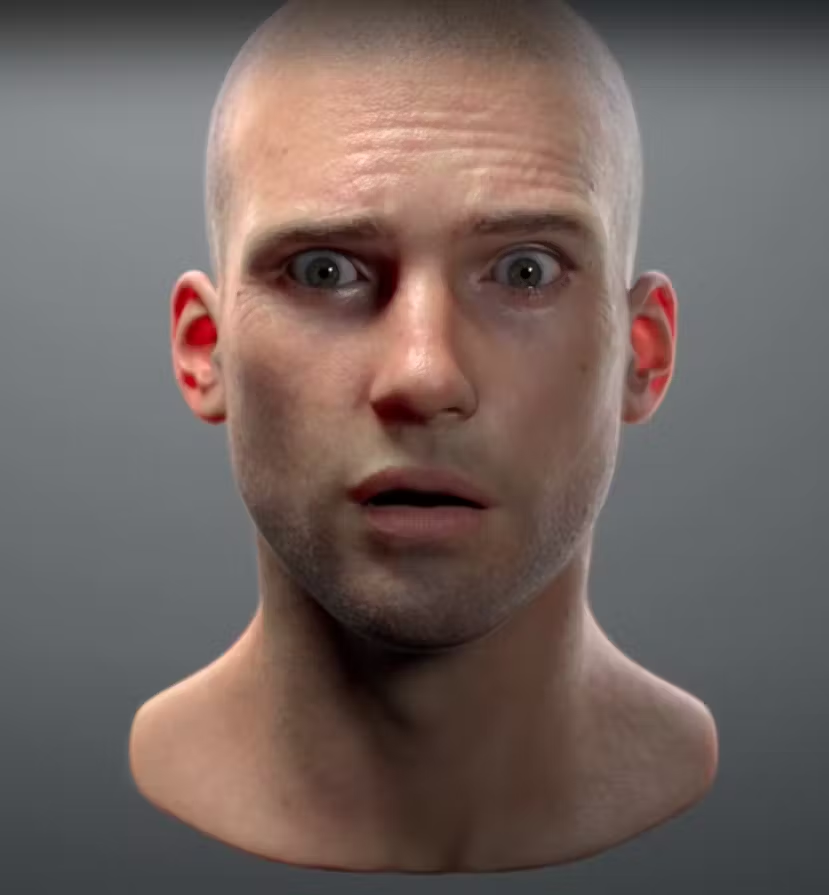
\includegraphics[height=5.8cm]{images/cgi}
		 \caption{\small Công nghệ CGI với người kỹ thuật số siêu thật \cite{edchrisjones}}
		\label{fig:CGI}
	\end{subfigure}
	\hfill
	\begin{subfigure}{0.6\textwidth}
		\centering
		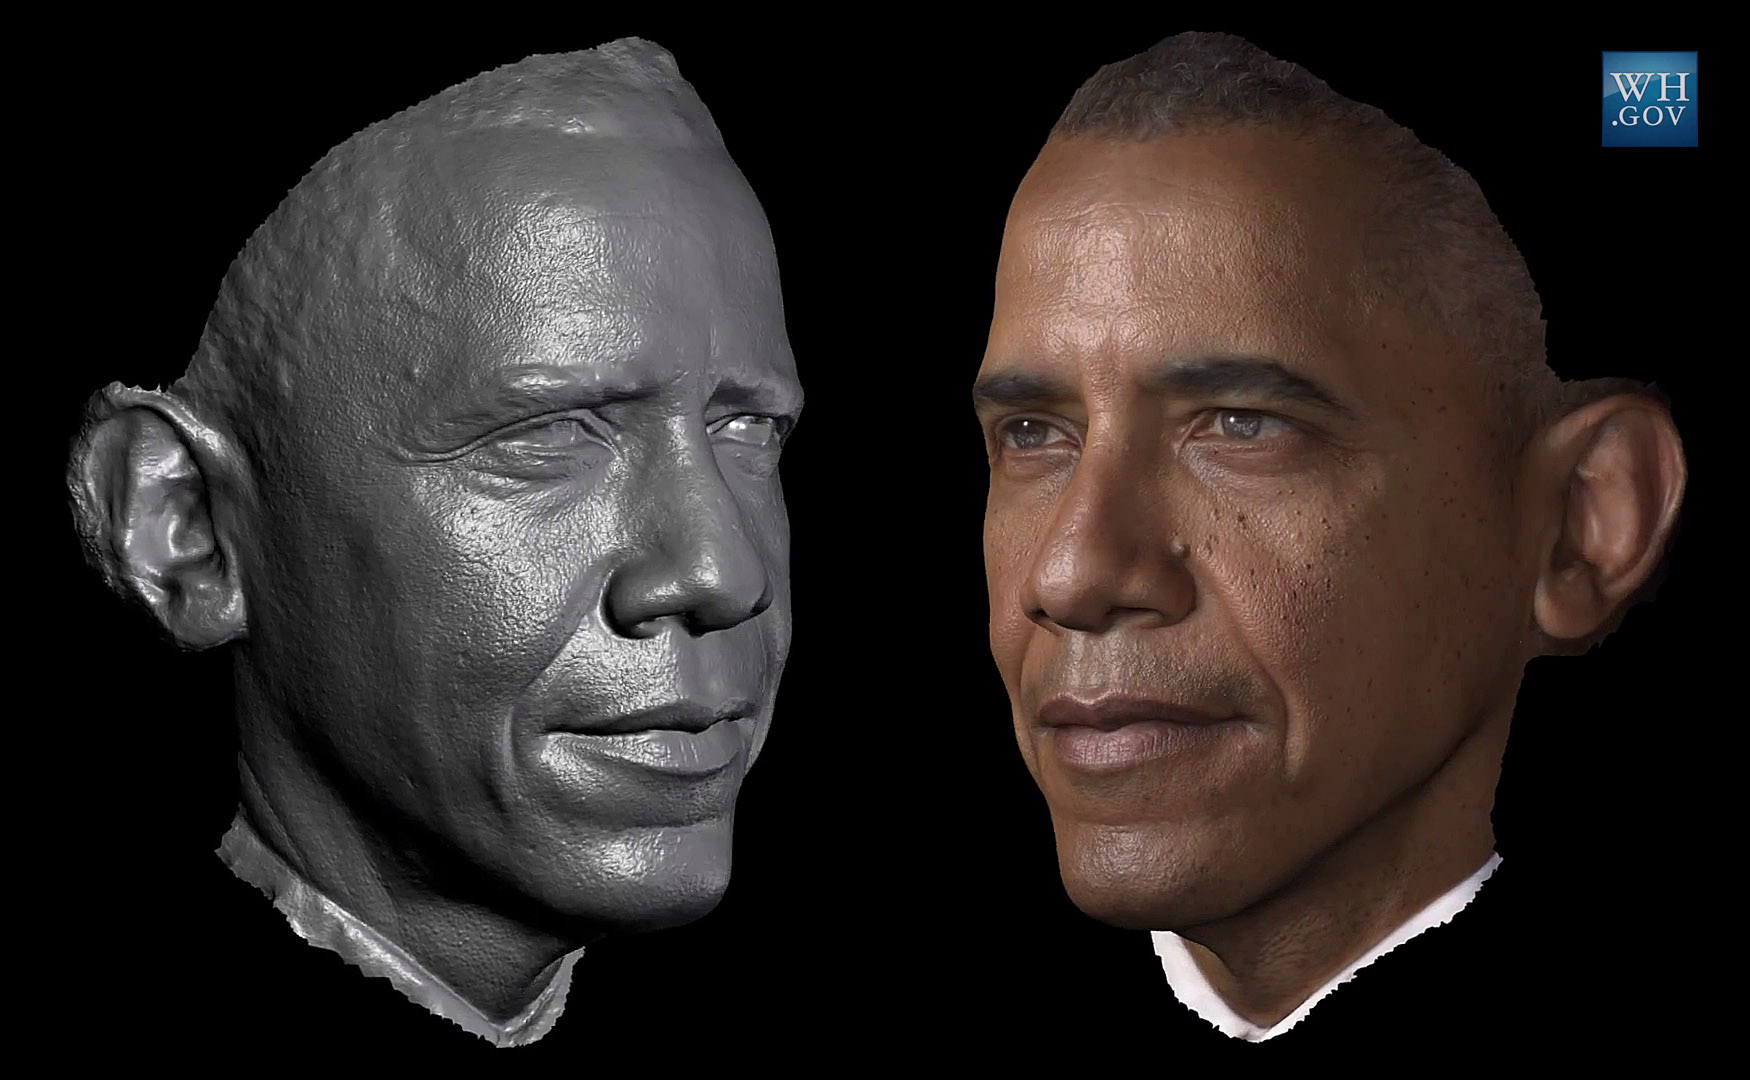
\includegraphics[height=5.8cm]{images/obama_scan}
		\caption{\small Minh họa công trình tái tạo khuôn mặt tổng thống Obama \cite{metallo2015scanning}}
		\label{fig:obamascan}
	\end{subfigure}
	\caption{Minh họa kỹ thuật đồ họa máy tính trong việc xây dựng người kỹ thuật số}
	\label{fig:DigitalHuman}
\end{figure}

Mỗi ngày, trên thế giới có hàng tỷ người nhìn vào màn hình RGB, kết quả hiển thị trên màn hình là đầu ra của mọi hệ thống phần mềm. Do đó, việc hiển thị từng pixel trên màn hình và cách để mô phỏng lại hình ảnh trên một cách chân thực nhất được các nhà khoa học về đồ họa máy tính (Computer Graphic) nghiên cứu từ những năm 1960s và đặc biệt là việc mô hình phỏng lại con người. Từ năm 2014, các họa sĩ 3D đã có thể tạo nên một nhân vật người siêu thật như \autoref{fig:CGI} trong khi đó các phần cứng máy tính còn chưa phát triển như hiện nay. 

Ngày nay, công nghệ đồ họa máy tính đã hoàn toàn có thể mô phỏng nhiều vật giống đến mức siêu thực (realistic), bao gồm các vật phức tạp như nước, đường xá, bánh mì,...  và thậm chí là cả cơ thể và khuôn mặt con người với độ chi tiết đến từng lông tơ, nốt mụn và vân mắt. 
Vào năm 2015, bằng kỹ thuật quét 3 chiều ghi lại toàn bộ các góc của khuôn mặt, sự phản chiếu ánh sáng, trong công trình \cite{metallo2015scanning}
các nhà khoa học đồ họa máy tính đã có thể tái tạo toàn bộ khuôn mặt của tổng thống Obama trên máy tính với độ chính xác cao và gần như không thể phân biệt \autoref{fig:obamascan}.

Trí tuệ nhân tạo thể hiện kết quả vượt bậc những năm gần đây, không chỉ trong nghiên cứu mà còn trong ứng dụng thực tế, tiêu biểu như ứng dụng ChatGPT, MidJourney và sự phát triển cả theo chiều dọc và chiều ngang trong nhiều lĩnh vực ứng dụng trí tuệ nhân tạo. Mặc dù đồ họa máy tính đã có thể xây dựng khuôn mặt người siêu thật, việc sinh cử chỉ lại phụ thuộc vào việc chụp chuyển động (Motion Capture) từ các cảm biến và gặp khó khăn khi xây dựng hệ thống trí tuệ nhân tạo học từ dữ liệu.

Các hệ thống trí tuệ nhân tạo hiện nay đã có thể tạo văn bản và giọng nói tiệm cận như con người, nhưng một trong những trở ngại lớn nhất để xây dựng con người kỹ thuật số hiện nay chính là việc sinh cử chỉ. Chính vì vậy, mục tiêu của luận văn là xây dựng một hệ thống sinh cử chỉ hội thoại dựa trên cảm xúc và ngữ nghĩa với dữ liệu đầu vào gồm cả văn bản và giọng nói.

\section{Động lực nghiên cứu}

Tổng hợp cử chỉ hội thoại giúp ích cho rất nhiều lĩnh vực như hoạt ảnh, dựng phim, trò chơi điện tử, giáo dục và những ứng dụng thực tế ảo. Việc tổng hợp cử chỉ chuyển động được thực hiện theo cách truyền thống là thuê các diễn viên sử dụng thiết bị theo dõi chuyển động và bố trí các hệ thống cảm biến xung quanh thu nhận chuyển động để đạt được độ chính xác chân thực nhất. Tuy nhiên, các chuyển động thu được sau đó chỉ được phát lại và không có sự biến đổi linh hoạt giữa các hành động. Do đó, việc áp dụng trí tuệ nhân tạo để có thể học các chuyển động từ dữ liệu thu nhận và sau đó có thể sinh ra dữ liệu mới sẽ là một cuộc cách mạng trong ngành công nghiệp chụp chuyển động.

Vào năm 2011, một nhóm tác giả \cite{bergmann2011relation} đã chứng minh rằng có sự liên hệ giữa giọng nói và cử chỉ con người, đây chính là tiền đề cho thấy chúng ta có thể dùng dữ liệu giọng nói để có thể dùng để học và biểu diễn được cử chỉ con người.
Với sự thành công của các mô hình ngôn ngữ tự nhiên trong xử lý văn bản và độ chính xác siêu thật trong việc mô phỏng gương mặt con người, ngành đồ họa máy tính đã đạt được những tiến bộ vượt bậc. Cùng với đó là sự dễ dàng và chính xác trong việc tổng hợp giọng nói con người.
Việc ứng dụng trí tuệ nhân tạo để sinh cử chỉ con người là một trong những điểm nghẽn chính trong phát triển trợ lý ảo giao tiếp và tương tác với con người.

\section{Dữ liệu bài toán}
\label{sec:Data}


\begin{figure}[H]
	\centering
	\begin{subfigure}{0.49\textwidth}
		\centering
		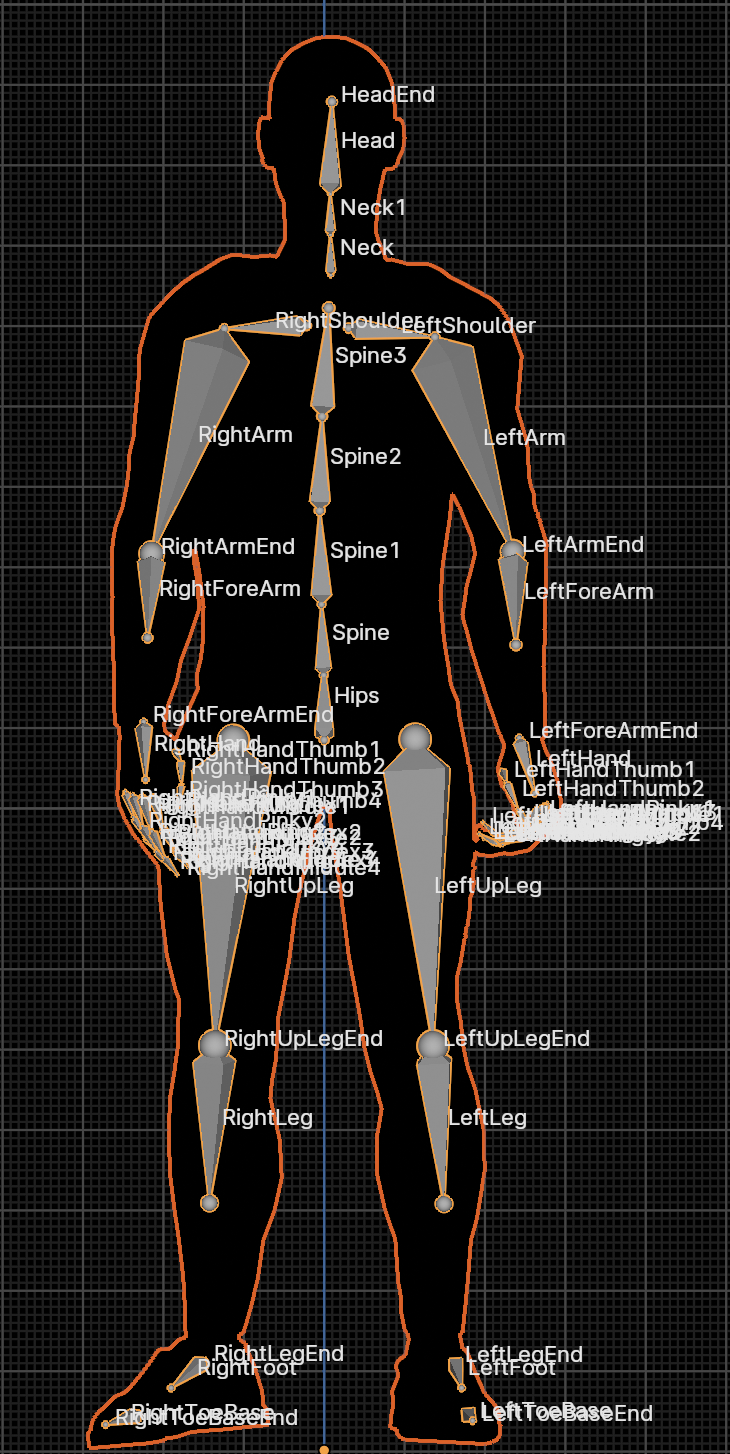
\includegraphics[height=10cm]{images/Skeleton.png}
		\caption{\small Khung xương và tên của các khớp của một khung xương trong mỗi khung hình.}
		\label{fig:Skeleton}
	\end{subfigure}
	\hfill
	\begin{subfigure}{0.49\textwidth}
		\centering
		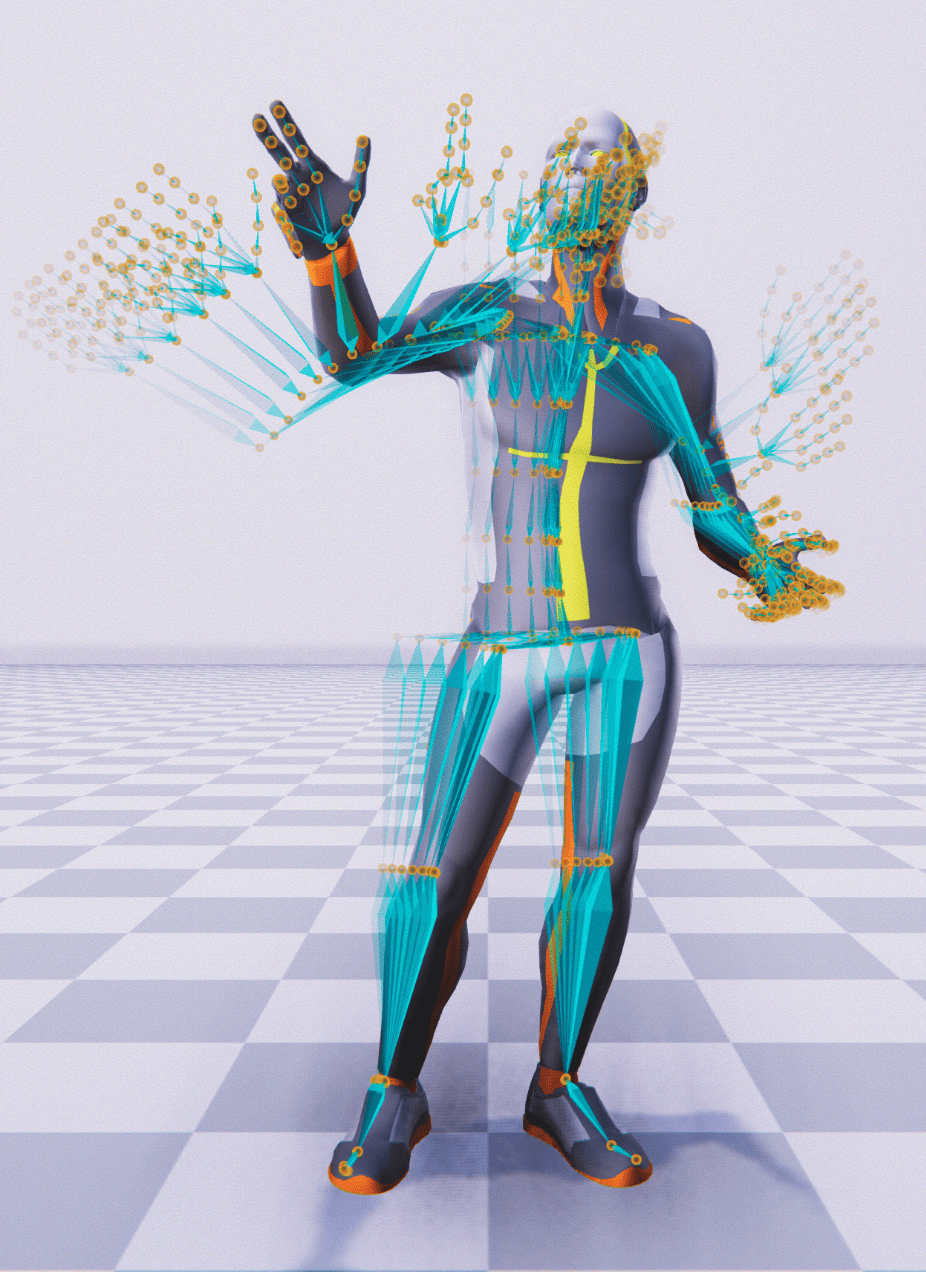
\includegraphics[height=10cm]{images/MotionPastAndFuture.png}
		\caption{\small Chuỗi chuyển động của cử chỉ bao gồm 6 cử chỉ quá khứ và 6 cử chỉ tương lai.}
		\label{fig:MotionPastAndFuture}
	\end{subfigure}
\end{figure}

\subsection{Kiến trúc khung xương của cử chỉ}

Cử chỉ (gesture) trong luận văn là sự chuyển động của toàn bộ cơ thể của một nhân vật như hình \autoref{fig:Skeleton} theo từng khung hình. Để có thể biểu diễn các chuyển động của một nhân vật trong đồ họa máy tính, các chuyển động sẽ được biểu diễn thành chuyển động của các xương (bone) riêng lẻ. Bao gồm cánh tay (hand), chân (leg), đầu (head), xương sống (spine),... Kiến trúc đầy đủ của một nhân vật được trình bày ở phụ lục \autoref{appendix:BVHData:skeleton}.

Dữ liệu một nhân vật theo thời gian trong thực tế sẽ được thu nhận bằng các hệ thống chụp chuyển động (motion capture) với các hệ thống camera và cảm biến chuyên biệt. Kết quả của quá trình motion capture là các tệp được định nghĩa dưới dạng tệp BVH (Biovision Hierarchy).

Các tệp BVH bao gồm hai thành phần chính: {HIERARCHY} và {MOTION}. HIERARCHY được thể hiện dưới dạng một cây bao gồm các thông tin về tên và vị trí khởi tạo các khung xương, MOTION là dữ liệu về chuyển động của toàn bộ khung xương theo từng khung hình (frame).  Mỗi tệp BVH sẽ có thông tin về số khung hình trên giây ($\text{fps}$) và tổng sống khung hình. Thông tin mỗi tệp BVH được trình bày ở phụ lục \autoref{appendix:BVHData:BVHStructure}. 


\subsection{Kiến trúc chuyển động của cử chỉ}

Dữ liệu chuyển động của cử chỉ như \autoref{fig:MotionPastAndFuture} hay phần MOTION của tệp BVH sẽ chứa thông tin về tọa độ và góc quay của một nhân vật theo từng khung hình. Dữ liệu mỗi khung hình là tập khung xương (skeleton) bao gồm $75$ xương (bone), $\{ \textbf{b}_{1}, \textbf{b}_{2}, \cdots , \textbf{b}_{75} \}$, mỗi xương thể hiện vị trí (position) $\{ p_{x}, p_{y}, p_{z} \}$ và góc quay (rotation) $\{ r_{x}, r_{y}, r_{z} \}$ chuyển động của một nhân vật theo thời gian.

Kết quả của việc sinh cử chỉ (gesture generation) là sinh ra chuỗi chuyển động góc quay các xương của nhân vật theo từng khung hình (frame). Việc sinh cử chỉ (gesture generation) được đánh giá bằng việc tạo ra các cử chỉ tự nhiên, giống con người (human-likeness) và phù hợp với ngữ cảnh.

Trong luận văn, các dữ liệu về vị trí và góc quay của khung xương nhân vật được tiền xử lý để chuyển thành một vector đặc trưng $\mathbf{g} \in \mathbb{R}^{D}$ với $D=1141$. Dữ liệu cần học khi đó sẽ là $\bx \in \mathbb{R}^{M \times D}$.

Quá trình xử lý dữ liệu được trình bày đầy đủ ở \autoref{appendix:BVHData}.

\section{Phát biểu bài toán}
\label{sec:ProblemStatement}

Với kết quả cuối cùng là chuỗi cử chỉ thể hiện sự chuyển động của các khung xương theo từng khung hình, thì có rất nhiều phương pháp khác nhau như phương pháp học phân loại (classification), gom nhóm (clustering), hồi quy (regression), .. . Trong luận văn này, sinh cử chỉ là  được cho bài toán hồi quy (regression), tạo ra dữ liệu mới dựa trên mô hình sinh, với đầu vào là một chuỗi cử chỉ cho trước và đầu ra là chuỗi cử chỉ tiếp theo cần dự đoán.
	
\begin{figure}[H]
	\centering
	\href{https://www.youtube.com/watch?v=B6nv1kQmi-Q}{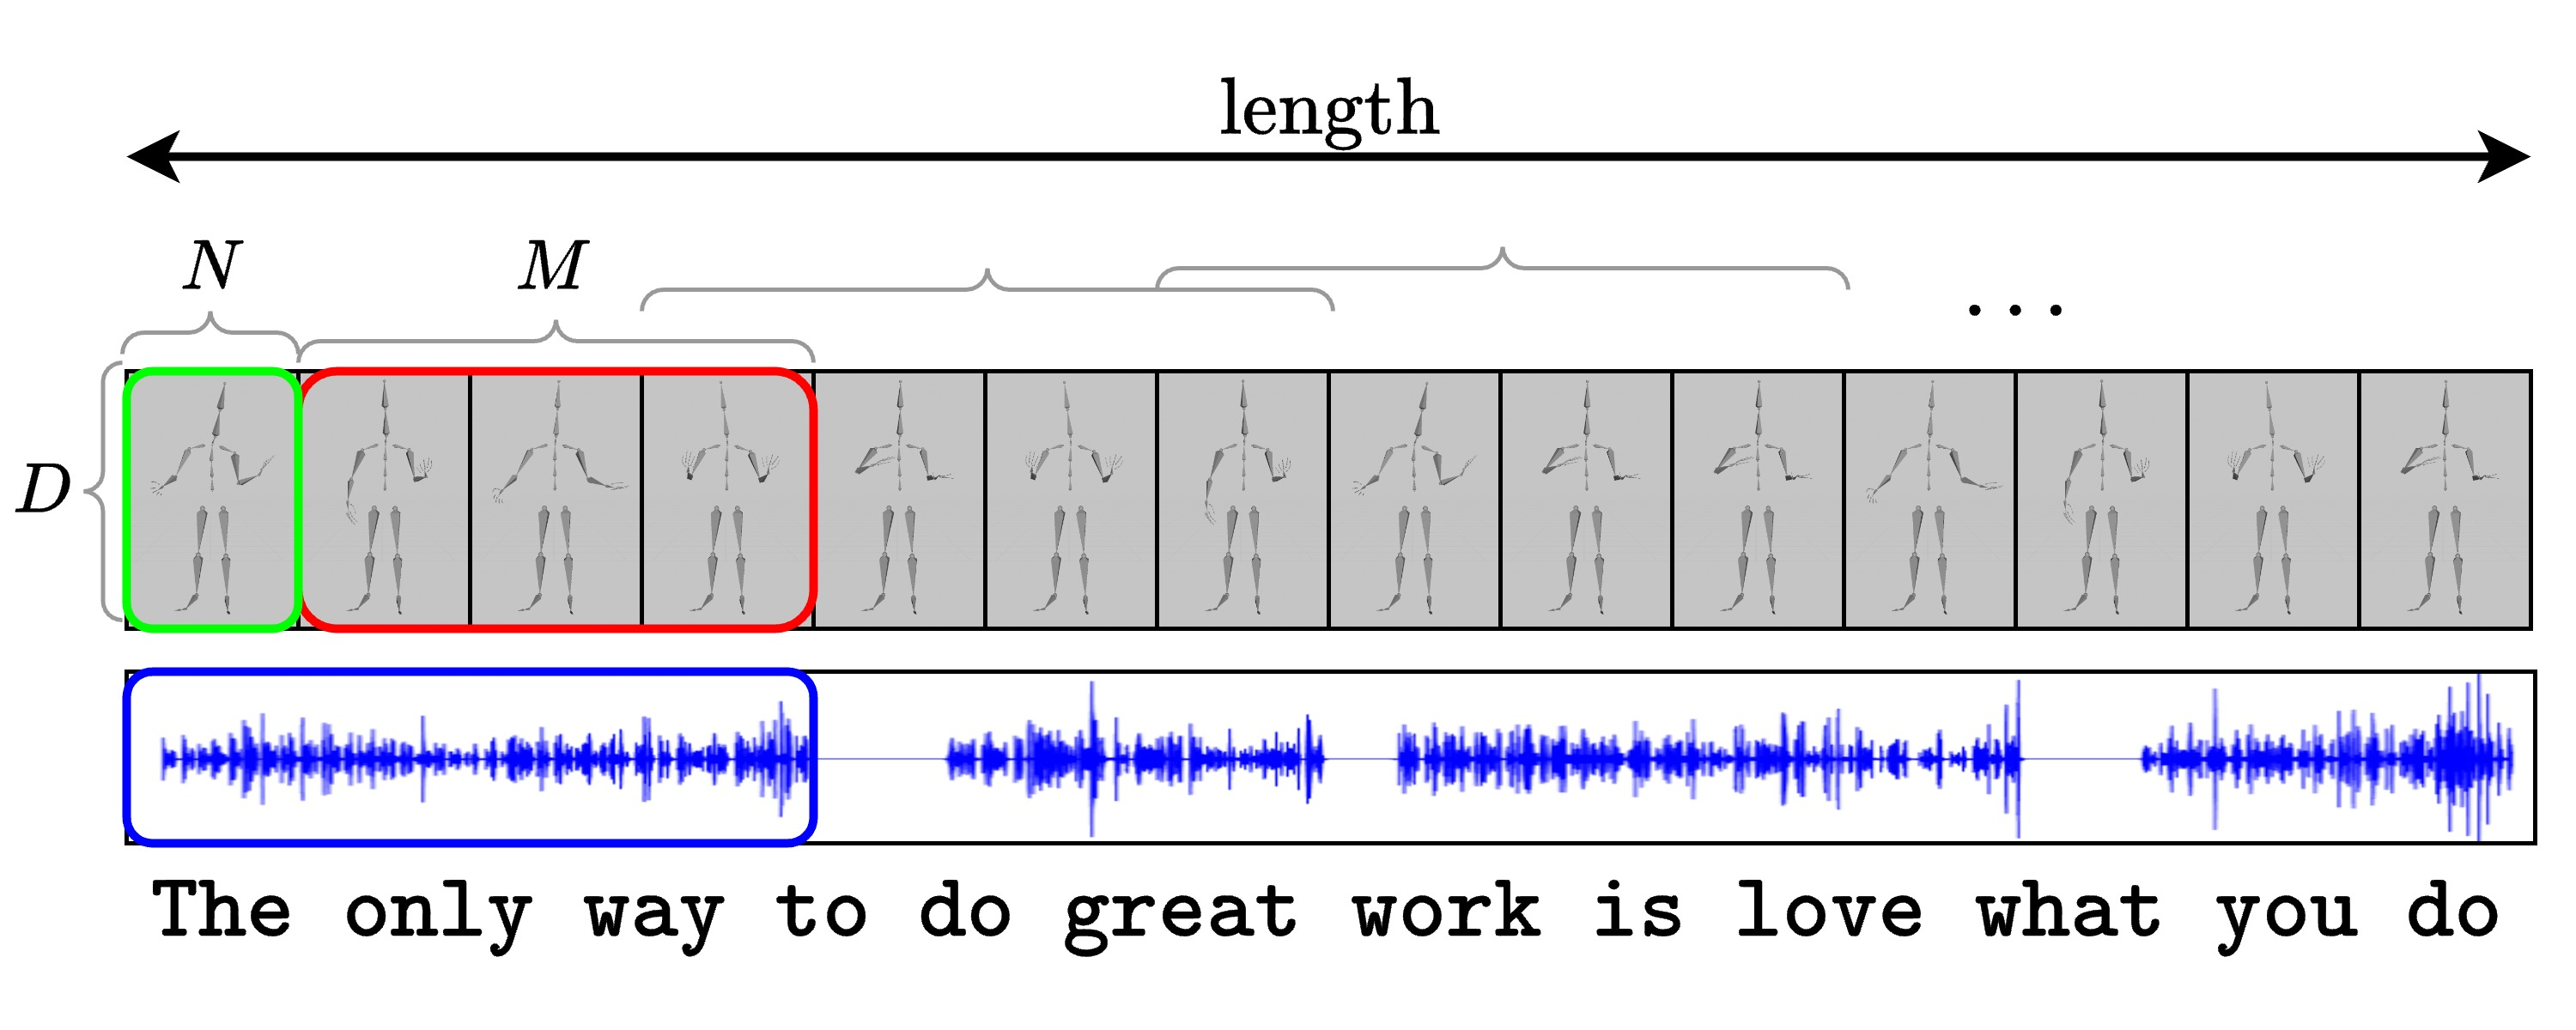
\includegraphics[width=\linewidth]{FeatureProcessing}}
	\caption{Minh họa một chuỗi cử chỉ, $N$ frame đầu được lấy làm cử chỉ khởi tạo $\mathbf{s}$ (seed gesture) và $M$ khung hình còn lại làm cử chỉ để học}
	\label{fig:GestureSeries}
\end{figure}

Với một chuỗi cử chỉ có độ dài khung hình bất kỳ, cảm xúc sẽ được gán cho toàn bộ chuỗi cử chỉ. Một phần cải tiến của luận văn là tương ứng với chuỗi cử chỉ là dữ liệu giọng nói và đoạn văn bản được dịch từ dữ liệu giọng nói tương ứng.
Mục tiêu của luận văn là xây dựng mô hình để dự đoán từng đoạn nhỏ, với thông tin dữ liệu đầu vào bao gồm chuỗi $N$ frame cử chỉ cho trước $\mathbf{s} \in \mathbb{R}^{1:N \times D}$ (seed gesture), chuỗi giọng nói $\mathbf{a}$ (speech), văn bản $\mathbf{v}$ (text),  cảm xúc $\mathbf{e}$ (emotion) tương ứng.

Kết quả dự đoán của mô hình là $\hat{\mathbf{x}} \in \mathbb{R}^{1:M \times D}$ bao gồm từ frame 1 đến frame $M$ chuỗi cử chỉ tiếp theo . Với dữ liệu gốc là chuỗi cử chỉ đã có $\mathbf{x}  \in \mathbb{R}^{1:M \times D}$.

\begin{multicols}{2}
	
\textbf{Đầu vào}

\begin{itemize}
	\item Chuỗi cử chỉ khởi tạo: $\mathbf{s} \in \mathbb{R}^{1:N \times D}$
	\item Chuỗi giọng nói: $\mathbf{a}$
	\item Văn bản: $\mathbf{v}$ 
	%				\in \mathbb{R}^{16000 M}
	%			trích xuất đặc trưng MFCC: $\mathbf{a} \in \mathbb{R}^{M \times C_{\text{mfcc}}}$
	\item Cảm xúc: $\mathbf{e}$ 
	
	{\small
		(\texttt{Happy},  \texttt{Sad},  \texttt{Neutral}, \texttt{Angry}, \texttt{Old}, \texttt{Funny})
	}
\end{itemize}

\columnbreak

\textbf{Dữ liệu dự đoán}
\vspace{-10pt}
\begin{itemize}
	\item Chuỗi cử chỉ dự đoán: $\hat{\mathbf{x}} \in \mathbb{R}^{1:M \times D}$
\end{itemize}

\textbf{Dữ liệu gốc}
\vspace{-10pt}
\begin{itemize}
	\item Chuỗi cử chỉ gốc: $ \mathbf{x}  \in \mathbb{R}^{1:M \times D}$
\end{itemize}

\end{multicols}

\section{Các khó khăn cần giải quyết}
\label{sec:difficult}

Có rất nhiều khó khăn trong việc xây dựng một mô hình có thể học được các đặc trưng cử chỉ hội thoại như con người.

Thứ nhất, \textit{dữ liệu không đủ nhiều và chất lượng}, chi phí để tạo ra một bộ dữ liệu trong ngành công nghiệp chụp chuyển động có chất lượng và quy mô lớn để ứng dụng thực tế là rất cao.

Thứ hai, \textit{sự thiếu đồng nhất về ngữ cảnh của các loại dữ liệu}, các bộ dữ liệu về văn bản thường nhiều hơn so với giọng nói, và cũng không rõ văn bản đó được tạo ra bởi ai. Sự đồng bộ giữa giọng nói và cảm xúc khi nói cũng thường thiếu trong tập dữ liệu. Ngoài ra, dữ liệu văn bản trong tập dữ liệu huấn luyện lại thuộc nhiều chủ đề đa dạng.
 
Thứ ba, \textit{sự phân bố không cân xứng về  dữ liệu giữa các loại đặc trưng cần học}. Các dữ liệu dùng cho nghiên cứu cử chỉ hiện nay thường tập trung vào ngôn ngữ Tiếng Anh, các cử chỉ có sự phân bố không cân xứng giữa các trạng thái như nói, hỏi, hoặc im lặng.

Thứ tư, \textit{chi phí tính toán với nhiều loại dữ liệu của mô hình là một thách thức lớn}. Với đầu vào của mô hình gồm nhiều loại dữ liệu như văn bản, tiếng nói và điểm 3D, cần nhiều lớp mã hóa cho từng loại dữ liệu, dẫn đến chi phí tính toán cao trong cả giai đoạn huấn luyện và suy luận. Nếu giảm thông tin dữ liệu đầu vào cũng sẽ giảm kết quả suy luận của mô hình khi sinh cử chỉ.

Cuối cùng, \textit{các bước xử lý cần được thực hiện tuần tự}, cách hiệu quả nhất để con người tương tác với máy tính là thông qua giọng nói và nhập từ bàn phím, tuy nhiên việc xử lý được văn bản và giọng nói để làm đầu vào cho mô hình phải thực hiện tuần tự. Độ trễ trong quá trình suy luận của sản phẩm thực tế cũng là một vấn đề lớn, vì người dùng không thể chờ đợi quá lâu để nhận kết quả. Ngoài ra, việc hiển thị cử chỉ đó lên máy tính bằng kỹ thuật đồ họa cũng cần được tối ưu để giảm thời gian xử lý.


\section{Đóng góp dự kiến}

\begin{itemize}
	\item Dựa trên tập dữ liệu có sẵn, luận văn chuyển giọng nói trong tập dữ liệu thành văn bản, và dùng văn bản đó để làm dữ liệu huấn luyện mới như là một dữ liệu ngữ nghĩa bổ sung trong quá trình học.
	
	\item Dựa trên mô hình cơ bản DiffuseStyleGesture, luận văn mở rộng thêm đặc trưng văn bản trong quá trình khử nhiễu có điều kiện.
	
	\item Luận văn sử dụng Unity để render, trích xuất dữ liệu và trực quan hóa kết quả sinh cử chỉ.
	
	\item Luận văn xây dựng hệ thống kết xuất, và minh họa chương trình bằng Unity
\end{itemize}


% Ngôn ngữ để viết và trình bày báo cáo khóa luận tốt nghiệp, đồ án tốt nghiệp, thực tập tốt nghiệp (sau đây gọi chung là báo cáo) là tiếng Việt hoặc tiếng Anh. 
% Trường hợp chọn ngôn ngữ tiếng Anh để viết và trình bày báo cáo,  sinh viên cần có đơn đề nghị, được cán bộ hướng dẫn (CBHD) đồng ý và nộp cho bộ phận Giáo vụ của Khoa vào thời điểm đăng ký đề tài để xin ý kiến.
% Báo cáo viết và trình bày bằng tiếng Anh phải có bản tóm tắt viết bằng tiếng Việt.


%Tóm tắt luận văn được trình bày nhiều nhất trong 24 trang in trên hai mặt giấy, cỡ chữ Times New Roman 11 của hệ soạn thảo Winword hoặc phần mềm soạn thảo Latex đối với các chuyên ngành thuộc ngành Toán.

%Mật độ chữ bình thường, không được nén hoặc kéo dãn khoảng cách giữa các chữ.
%Chế độ dãn dòng là Exactly 17pt.
%Lề trên, lề dưới, lề trái, lề phải đều là 1.5 cm.
%Các bảng biểu trình bày theo chiều ngang khổ giấy thì đầu bảng là lề trái của trang.
%Tóm tắt luận án phải phản ảnh trung thực kết cấu, bố cục và nội dung của luận án, phải ghi đầy đủ toàn văn kết luận của luận án.
%Mẫu trình bày trang bìa của tóm tắt luận văn (phụ lục 1).


\chapter{TỔNG QUAN}
\label{Chapter2}

Bài toán sinh cử chỉ cũng tương tự như các bài toán khác đều đã nghiên cứu và phát triển song hành với các phương pháp học máy truyền thống và hiện đại. Gồm các nhóm phương pháp dựa trên luật và các phương pháp dựa trên dữ liệu.  Đầu tiên luận văn chứng minh mối quan hệ giữa cử chỉ và giọng nói \ref{sec:relationspeechandgesture}, từ đó là tiền đề thể hiện sự đồng bộ về dữ liệu giữa cử chỉ và giọng nói và việc học mối quan hệ giữa cử chỉ và giọng nói có ý nghĩa. Trong mục \ref{sec:commonstage} Luận văn sẽ trình bày về các công đoạn chung trong các phương pháp sinh cử chỉ.
Ở phần \ref{sec:relatedwork} luận văn trình bày về các phương pháp đã được sử dụng trong quá trình sinh cử chỉ. Luận văn sẽ so sánh các phương pháp, từ đó nêu lý do luận văn sử dụng mô hình diffusion để áp dụng cho bài toán sinh cử chỉ.
Trong phần \ref{sec:diffusionbase}, luận văn sẽ trình bày về cách các mô hình diffusion được áp dụng cho bài toán sinh cử chỉ gần đây.

\section{Mối quan hệ giữa cử chỉ và giọng nói}
\label{sec:relationspeechandgesture}

Theo ngôn ngữ học, cử chỉ có thể được phân thành 6 nhóm chính: cử chỉ thích nghi (adaptors), cử chỉ biểu tượng (emblems), cử chỉ chỉ định (deictics), cử chỉ biểu trưng (iconics), cử chỉ ẩn dụ (metaphorics), và cử chỉ nhấn mạnh (beat) \cite{ekman1969repertoire}, \cite{sebeok2011advances}. Trong số đó, cử chỉ nhấn mạnh không mang ý nghĩa ngữ nghĩa trực tiếp nhưng đóng vai trò quan trọng trong việc đồng bộ nhịp điệu giữa giọng nói và cử chỉ \cite{kipp2005gesture}, \cite{sebeok2011advances}. Tuy nhiên, nhịp điệu giữa giọng nói và cử chỉ nhấn mạnh không hoàn toàn đồng bộ, khiến việc học mối quan hệ thời gian giữa chúng trở nên phức tạp \cite{mcclave1994gestural}, \cite{bhattacharya2021speech2affectivegestures}, \cite{kucherenko2020gesticulator}, \cite{yoon2020speech}.

Cử chỉ tương tác với các cấp độ thông tin khác nhau trong giọng nói \cite{sebeok2011advances}. Chẳng hạn, cử chỉ biểu tượng, như hành động giơ ngón cái, thường liên quan đến thông tin ngữ nghĩa cấp cao (ví dụ: "tốt" hoặc "tuyệt vời"), trong khi cử chỉ nhấn mạnh thường đi kèm với thông tin cấp thấp như nhấn mạnh trong âm thanh. Các nghiên cứu trước đây thường chỉ sử dụng đặc trưng từ lớp cuối cùng của bộ mã hóa giọng nói để tổng hợp cử chỉ \cite{alexanderson2020style}, \cite{bhattacharya2021speech2affectivegestures}, \cite{kucherenko2021large}, \cite{qian2021speech}, \cite{yoon2022genea}. Tuy nhiên, cách tiếp cận này có thể làm trộn lẫn thông tin từ nhiều cấp độ, dẫn đến khó khăn trong việc phân tách rõ ràng nhịp điệu và ngữ nghĩa.

Như các nghiên cứu ngôn ngữ học chỉ ra \cite{kipp2005gesture}, \cite{neff2008gesture}, \cite{webb1997linguistic}, cử chỉ trong giao tiếp hàng ngày có thể được chia thành một số lượng giới hạn các đơn vị ngữ nghĩa với các biến thể chuyển động khác nhau. Dựa trên giả định này, được phân tách đặc trưng giọng nói thành hai loại: đặc trưng cấp cao đại diện cho các đơn vị ngữ nghĩa, và đặc trưng cấp thấp xác định các biến thể chuyển động. Từ đó, mối liên hệ giữa chúng được học thông qua các lớp khác nhau của bộ mã hóa giọng nói. Các thử nghiệm chứng minh rằng cơ chế này có khả năng tách biệt rõ ràng các đặc trưng ở nhiều cấp độ, đồng thời tổng hợp được cử chỉ phù hợp về ngữ nghĩa và phong cách.


\section{Các công đoạn chung trong bài toán sinh cử chỉ}
\label{sec:commonstage}

\begin{figure}[H]
	\centering
	\includegraphics[width=\textwidth]{CommonStage}
	\caption{Các công đoạn trong mô hình sinh cử chỉ cử chỉ.}
	\label{fig:CommonStage}
\end{figure}

\section{Tổng quan các phương pháp cho bài toán sinh cử chỉ}
\label{sec:relatedwork}



\subsection{Phương pháp dựa trên luật}

Các phương pháp dựa trên luật thường ánh xạ (mappings) từng giọng nói với từng đơn vị cử chỉ \cite{huang2012robot}. Và luật được tạo thủ công. Phương pháp dựa trên luật thì chúng ta có thể dễ dàng điều khiển kết quả của mô hình và có khả năng giải thích tốt kết quả dự đoán của mô hình.
Tuy nhiên chi phí để tạo thủ công là không khả thi để xây dựng cho các ứng dụng phức tạp đòi hỏi phải xử lý một lượng dữ liệu rất lớn.

\subsection{Phương pháp dựa trên thống kê}

Tương tự như phương pháp dựa trên luật, phương pháp dựa trên dữ liệu cũng ánh xạ các đặc trưng của giọng nói tương ứng với cử chỉ nhưng thay vì làm thủ công thì được sử dụng học một cách tự động dựa trên dữ liệu.
Trong đó có hai phương pháp chính là phương pháp thống kê và phương pháp dựa trên dữ liệu.

%\subsubsection{Phương pháp thống kê}

Phương pháp thống kê sử dụng phân phối xác suất để tìm sự tương đồng giữa các đặc trưng giọng nói và cử chỉ \cite{levine2010gesture}. Tác giả \cite{neff2008gesture} xây dựng mô hình để học từng phong cách của từng người nói.

\subsection{Phương pháp học sâu}

\setcounter{figure}{3}
\begin{figure}[H]
	\centering
	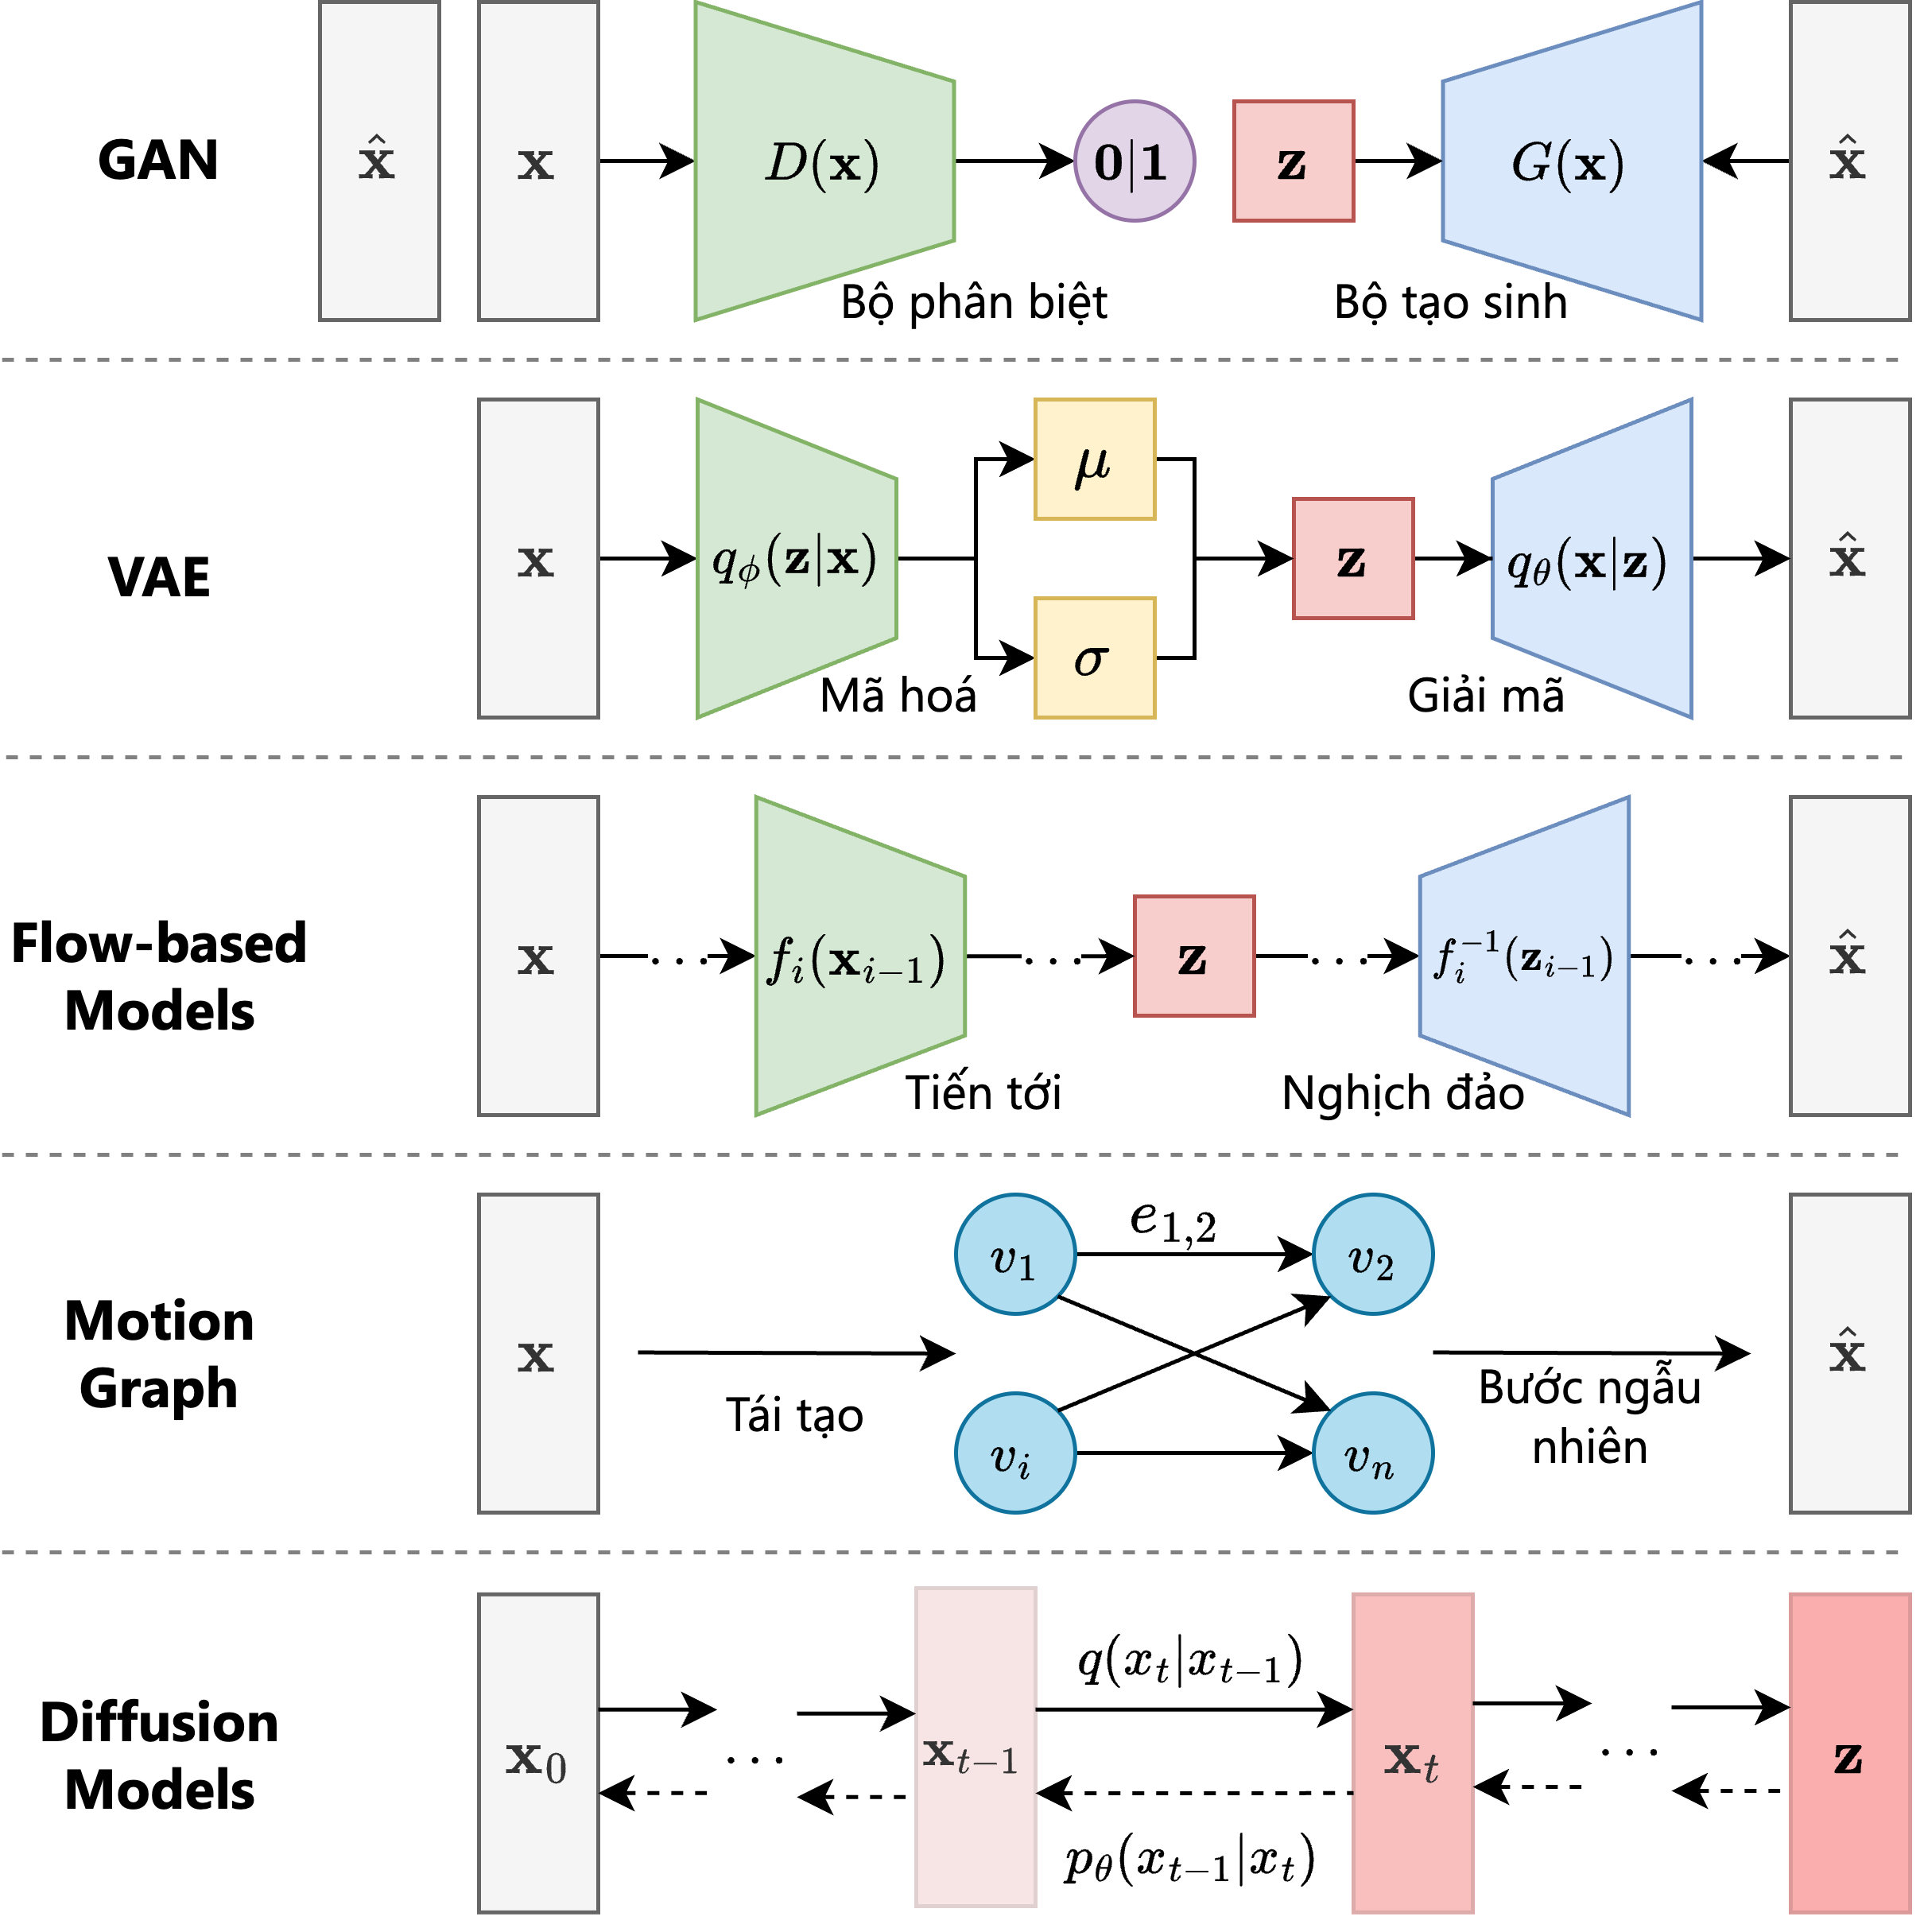
\includegraphics[width=0.8\textwidth]{GeneralOverview}
	\caption{Tổng quan về các mô hình tạo sinh khác nhau.}
	\label{fig:GeneralOverview}
\end{figure}

Phương pháp sinh cử chỉ được chia thành hai nhóm chính. Bao gồm các mô hình ước lượng log likelihood (likelihood-based model)  và phương pháp dựa vào các mô hình sinh ngầm định (implicit generative models) \cite{song2021score}. 

\subsubsection{Likelihood-based Model}

Phương pháp học ước lượng log likelihood là phương pháp học trực tiếp từ hàm mật độ xác xuất (probability density) thông qua maximum likelihood. Các phương pháp điển hình là autoregressive models, normalizing flow models, energy-based models (EBMs)
, và variational auto-encoders (VAEs).

%Phương pháp học sâu sử dụng mạng nơ-ron (neural) thông qua nhiều lớp ẩn để học một cách tự động các phối xác xuất giữa cử chỉ và giọng nói.

Mô hình được kết hợp với văn bản đầu vào được gắn thẻ với chủ đề, trọng tâm câu và thành ngữ để tạo ra các kịch bản cử chỉ, sau đó được ánh xạ sang một chuỗi các cử chỉ được chọn từ một từ điển hoạt họa. \cite{chiu2015predicting} huấn luyện một model classifier neural network để chọn một đơn vị cử chỉ phù hợp dựa trên đầu vào là giọng nói. 
%Nghiên cứu gần đây đã bắt đầu tận dụng học sâu và huấn luyện các mô hình kết thúc đến cuối sử dụng dữ liệu cử chỉ thô trực tiếp, giải phóng các nỗ lực thủ công trong thiết kế từ điển cử chỉ và các quy tắc ánh xạ.

Cử chỉ có thể được tổng hợp bằng các mô hình xác định như perceptron đa tầng (MLP) \cite{kucherenko2020gesticulator}, recurrent neural networks \cite{bhattacharya2021speech2affectivegestures}, \cite{liu2022learning}, \cite{hasegawa2018evaluation}, \cite{yoon2020speech}, convolutional networks \cite{habibie2021learning} và transformer \cite{bhattacharya2021text2gestures} 

\subsubsection{Implicit Generative Models}

Trong các phương pháp dựa vào mô hình sinh ngầm định, phân phối của dữ liệu được học một cách ngầm định thông qua việc quá trình lấy mẫu (sampling). Ví dụ tiêu biểu nhất là mô hình generative adversarial networks (GANs). Khi dữ liệu được tổng hợp bằng cách chuyển phân phối dữ liệu ban đầu ở dạng phân phối chuẩn về phân phối của dữ liệu.

%
%\begin{table}[h!]
%	\small
%	\centering
%	\renewcommand{\arraystretch}{1.5} % Tăng khoảng cách giữa các hàng
%	\begin{tabular}{|p{0.2\textwidth}|p{0.35\textwidth}|p{0.35\textwidth}|}
%		\hline
%		\textbf{Loại phương pháp} & \textbf{Ưu điểm} & \textbf{Nhược điểm} \\ \hline
%		Rule-Based  & 
%		- Dễ hiểu và dễ triển khai. \newline 
%		- Dễ giải thích và có thể kiểm soát được \newline
%		- Hiệu quả trong các trường hợp đơn giản hoặc dữ liệu nhỏ. & 
%		- Không tổng quát hoá tốt với dữ liệu phức tạp. \newline 
%		- Đòi hỏi nhiều công sức trong việc xây dựng quy tắc thủ công. \\ \hline
%		Likelihood-Based Models & 
%		- Khả năng ước lượng mật độ xác suất của dữ liệu \newline 
%		- Có khả năng mở rộng và học từ dữ liệu lớn & 
%		- Dễ bị ảnh hưởng bởi nhiễu \newline 
%		- Kết quả thấp ở vùng dữ liệu hiếm \newline
%		- Khả năng sinh không đa dạng \\ \hline
%		Implicit Generative Models & 
%		- Tạo ra dữ liệu chất lượng cao. \newline 
%		- Linh hoạt và đa dạng \newline
%		- Phủ được vùng có mật độ dữ liệu thấp & 
%		- Cần cấu hình phức tạp để đạt hiệu năng tốt. \newline 
%		- Khó đánh giá do mỗi lần nhiễu là khác nhau. \newline 
%		- Quá trình lấy mẫu chậm \\ \hline
%	\end{tabular}
%	\caption{Bảng so sánh ưu và nhược điểm của các phương pháp}
%\end{table}

\begin{table}[h!]
	\small
	\centering
	\renewcommand{\arraystretch}{1.5} % Tăng khoảng cách giữa các hàng
	\resizebox{\textwidth}{!}{ % Giảm kích thước bảng để vừa với trang
		\begin{tabular}{|p{0.2\textwidth}|p{0.35\textwidth}|p{0.35\textwidth}|p{0.2\textwidth}|}
			\hline
			\textbf{Phương pháp tiêu biểu} & \textbf{Ưu điểm} & \textbf{Nhược điểm} & \textbf{Loại phương pháp} \\ \hline
			Robot behavior toolkit \cite{huang2012robot} & 
			- Dễ hiểu và dễ triển khai. \newline 
			- Dễ giải thích và có thể kiểm soát được \newline
			- Hiệu quả trong các trường hợp đơn giản hoặc dữ liệu nhỏ. & 
			- Không tổng quát hoá tốt với dữ liệu phức tạp. \newline 
			- Đòi hỏi nhiều công sức trong việc xây dựng quy tắc thủ công. & 
			Rule-Based  \\ \hline
			MLP \cite{kucherenko2020gesticulator}, RNN \cite{bhattacharya2021speech2affectivegestures}, \cite{liu2022learning}, \cite{hasegawa2018evaluation}, \cite{yoon2020speech}, CNN \cite{habibie2021learning}, Transformer \cite{bhattacharya2021text2gestures}  & 
			- Khả năng ước lượng mật độ xác suất của dữ liệu \newline 
			- Có khả năng mở rộng và học từ dữ liệu lớn & 
			- Dễ bị ảnh hưởng bởi nhiễu \newline 
			- Kết quả thấp ở vùng dữ liệu hiếm \newline
			- Khả năng sinh không đa dạng & 
			Likelihood-Based Models \\ \hline
			\textbf{DiffusionStyle-Gesture} \cite{yang2022DiffuseStyleGestureplus}, MDM \cite{tevet2022human}, Motiondiffuse \cite{zhang2022motiondiffuse} &
			- Tạo ra dữ liệu chất lượng cao. \newline 
			- Linh hoạt và đa dạng \newline
			- Phủ được vùng có mật độ dữ liệu thấp & 
			- Cần cấu hình phức tạp để đạt hiệu năng tốt. \newline 
			- Khó đánh giá do mỗi lần nhiễu là khác nhau. \newline 
			- Quá trình lấy mẫu chậm & 
			Implicit Generative Models \\ \hline
		\end{tabular}
	}
	\caption{Bảng so sánh ưu và nhược điểm của các phương pháp}
\end{table}

%Trong mục tiêu theo luận văn sẽ trình bày các phương pháp sử dụng mô hình Diffusion.

%chuyển phân phối của dữ liệu ở dạng phân phối chuẩn hay ở một vị trí bất kỳ về phân phối chuẩn bằng hàm neuron network. 


%WGAN \cite{wu2021probabilistic}.



%\textbf{Bảng so sánh các phương pháp}
%
%\begin{table}[ht]
%	\centering
%	\begin{tabular}{|l|l|l|l|l|l|}
%		\hline
%		\textbf{Phương pháp} & \textbf{Loại mô hình} & \textbf{Đặc điểm nổi bật} & \textbf{Ưu điểm} & \textbf{Hạn chế} & \textbf{Tài liệu tham khảo} \\ \hline
%		VAE  & Autoencoder & Biểu diễn dữ liệu trong không gian tiềm ẩn & Tạo đặc trưng ẩn & Khó kiểm soát đầu ra & \cite{kingma2013auto} \\ \hline
%		VQ-VAE & Autoencoder (cải tiến) & Dùng codebook cho không gian tiềm ẩn & Biểu diễn chi tiết hơn & Phức tạp hơn & \cite{van2017neural} \\ \hline
%		RNN & Mạng hồi tiếp & Xử lý chuỗi dữ liệu & Tốt cho dữ liệu tuần tự & Khó huấn luyện & \cite{bhattacharya2021speech2affectivegestures} \\ \hline
%		Transformer & Mạng chú ý & Tạo cử chỉ qua cơ chế chú ý & Hiệu quả với dữ liệu dài & Yêu cầu nhiều tài nguyên & \cite{bhattacharya2021text2gestures} \\ \hline
%		WGAN & GAN & Học phân phối dữ liệu đối kháng & Tạo sự đa dạng & Khó huấn luyện & \cite{wu2021probabilistic} \\ \hline
%		Normalizing Flow & Mô hình xác suất & Học phân phối phức tạp & Hữu ích với dữ liệu phức tạp & Cần tài nguyên tính toán lớn & \cite{alexanderson2020style} \\ \hline
%		Diffusion Models & Mô hình sinh dữ liệu & Chi tiết cao, xử lý dữ liệu thiếu & Tạo cử chỉ chi tiết & Thời gian huấn luyện lâu & \cite{xu2022freeform} \\ \hline
%	\end{tabular}
%	\caption{So sánh các phương pháp sinh cử chỉ}
%\end{table}

%

\section{Diffusion-base Model}
\label{sec:diffusionbase}



Với đặc điểm dữ liệu là giá trị của các góc quay, các toạ độ của điểm khớp, nên cần độ chi tiết cao để tạo ra sự chân thực trong các chuyển động của nhân vật. Ngoài ra dữ liệu sẽ thiếu và rất ít dữ liệu trong các trường hợp cực trị của tham số.
Nên luận văn sử dụng mô hình Diffusion, với đặc điểm là có thể học được độ chi tiết cao hơn và có thể phủ được dữ liệu trong các trường hợp cực trị của tham số và độ phủ về mật độ dữ liệu thấp.



%❖ Chương này tập trung trình bày chi tiết những gì bạn
%làm
%❖ Mô tả chi tiết phương pháp thực hiện, giải pháp đề xuất, ứng dụng phát triển
%❖ Có thể đưa ra ví dụ minh họa để dẫn nhập
%❖ Nên phân thành các mục con
%   
%❖ Hướng nghiên cứu: Phương pháp đề xuất (Proposed Approach)
%o Cơ sở lý thuyết
%o Câu hỏi nghiên cứu, giả thuyết khoa học
%o Phương pháp/Thủ tục thực hiện nghiên cứu (procedure)
%o Đối tượng nghiên cứu
%o Môi trường (phần mềm, thư viện, máy móc, công cụ, v.v...)
%o Mô tả dữ liệu, quá trình thu thập dữ liệu
%o Độ đo để đánh giá (performance metrics)

%\chapter{PHƯƠNG PHÁP ĐỀ XUẤT}
\chapter{PHƯƠNG PHÁP NGHIÊN CỨU}
\label{chap:Chapter3}

Bản chất của các phương pháp dựa trên neural network là ước lượng xác xuất của dữ liệu (probability density) nên cần chuẩn hoá (normalization), trong khi mô hình Diffusion sẽ học để có thể ước lượng đạo hàm của phân phối dữ liệu \cite{song2021score} (estimating gradients of data distribution) và không phải chuẩn hoá trên toàn bộ dữ liệu, nên có kết quả tốt hơn so với các phương pháp neuron network không sử dụng diffusion. Mô hình diffusion có khả năng mô phỏng phân phối dữ liệu trong các trường hợp mật độ phân phối của dữ liệu thấp và có thể sinh được kết quả với độ chi tiết cao.

Mô hình của luận văn dựa trên mô hình DiffuseStyleGesture \cite{yang2022DiffuseStyleGestureplus} với cải tiến chính là dựa trên dữ liệu giọng nói, luận văn chuyển giọng nói thành văn bản và nhúng văn bản để được các vector đặc trưng văn bản, và sử dụng như là một vector đặc trưng về ngữ nghĩa trong quá trình diffusion có điều kiện. Quá trình này được trình bày \autoref{subsec:feature_extraction}. Ngoài ra ở công đoạn \textit{7. Kết xuất}  (\autoref{fig:CommonStage}), luận văn sử dụng Unity để kết xuất văn bản. Các đóng góp chính của luận văn được trình bày đầy đủ ở \autoref{sec:contribution}.

Trước tiên luận văn trình bày về mô hình diffusion \autoref{sec:summary_diffusion}, và phần \autoref{sec:ohgesture} sẽ trình bày về mô hình đề xuất OHGesture. 

%Diffusion \cite{ho2020denoising} là mô hình được lấy cảm hứng từ mô hình khuếch tán các chất trong hóa học.

\section{Mô hình diffusion cơ bản và các cải tiến}
\label{sec:summary_diffusion}

%\subsection{Quá trình gây nhiễu và khử nhiễu không huấn luyện}

\begin{figure}[H]
	\centering
	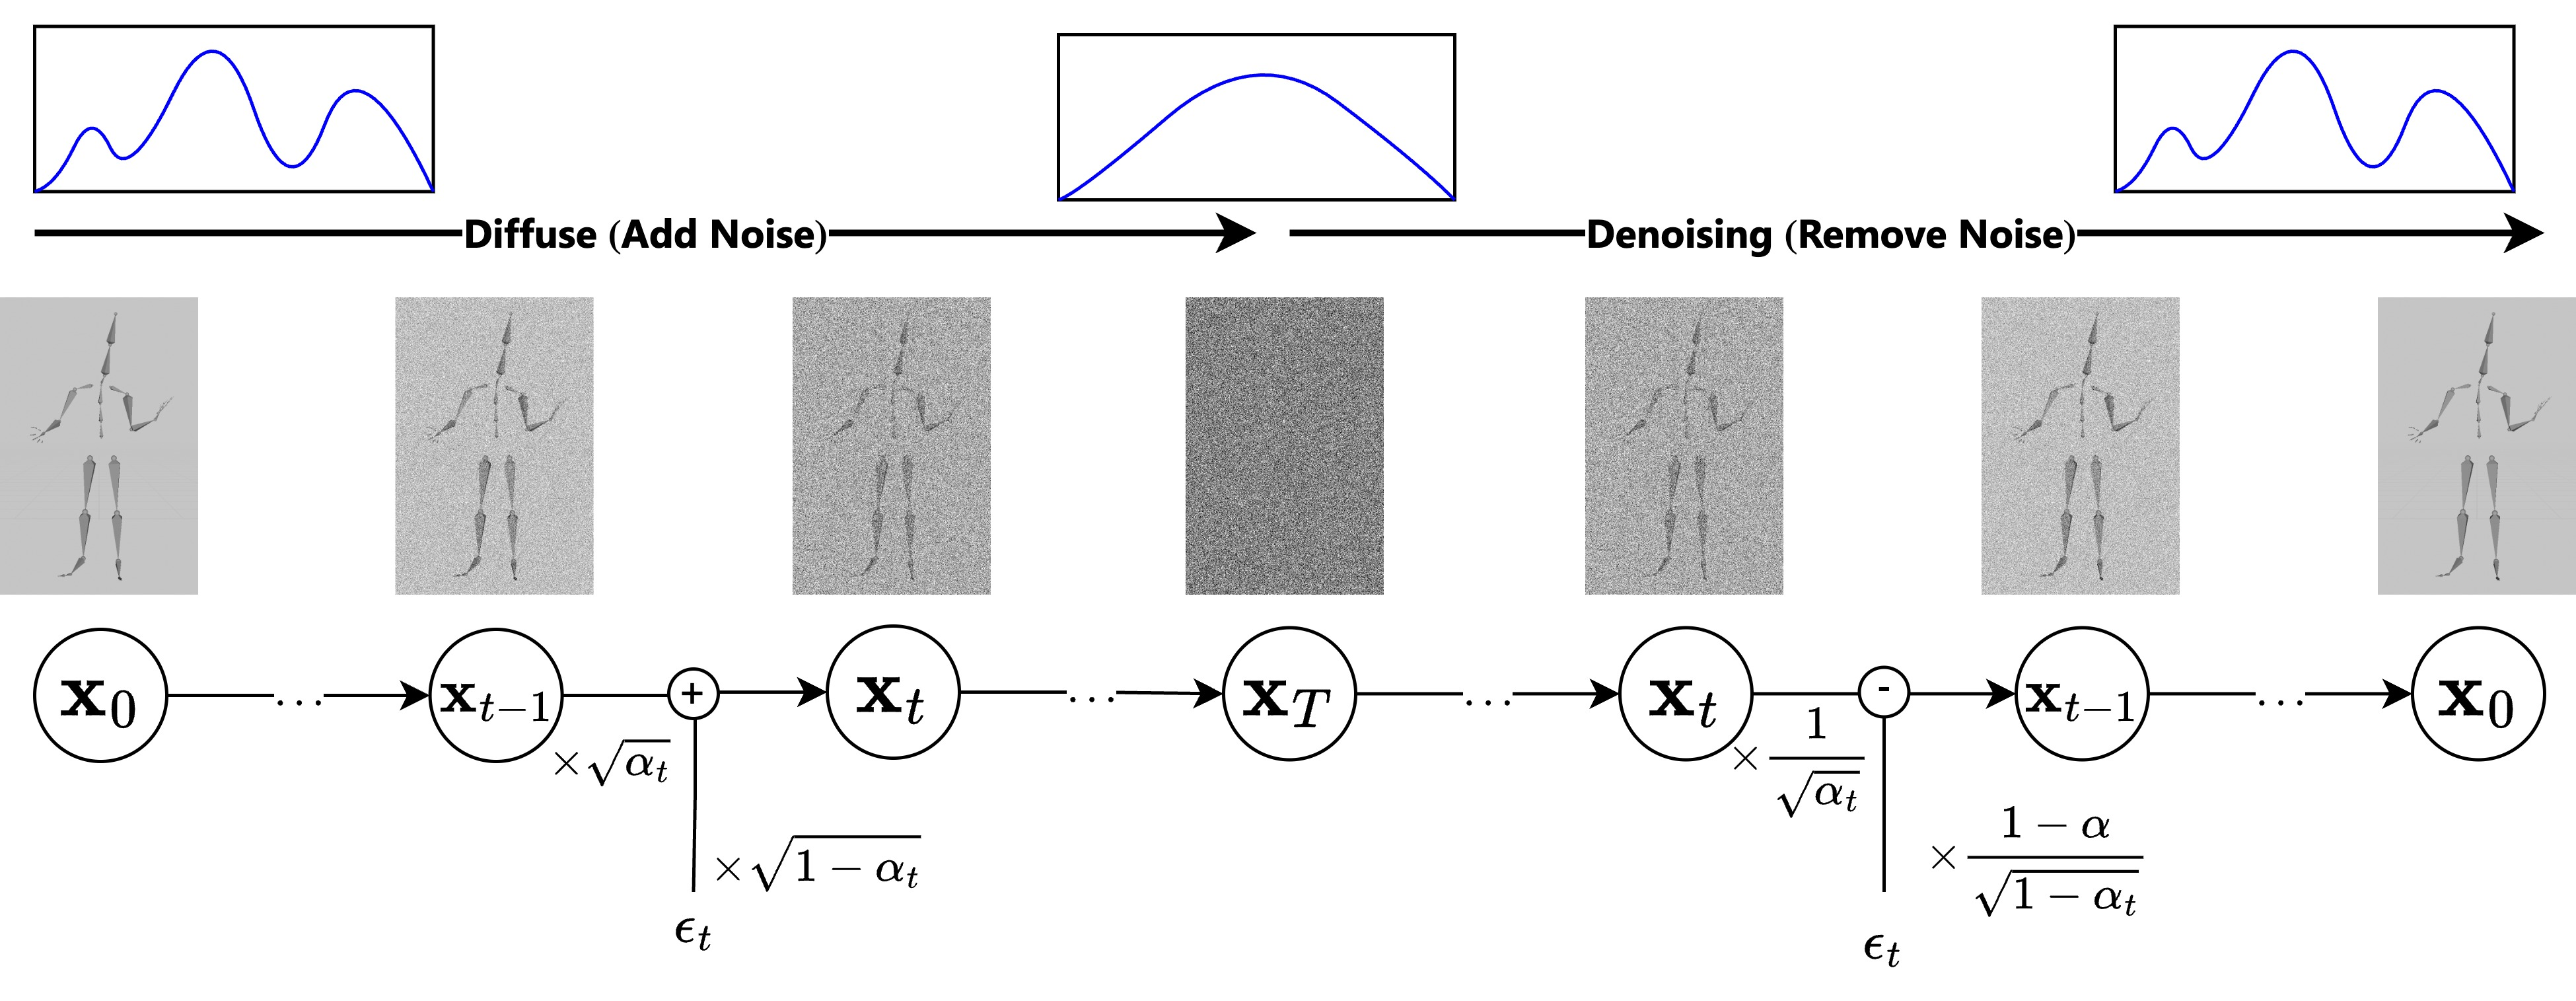
\includegraphics[width=\linewidth]{DiffuseAndDenoise}
	\caption{Quá trình gây nhiễu (Diffuse) và khử nhiễu (Denoise) \textbf{không} huấn luyện}
	\label{fig:DiffuseAndDenoise}
\end{figure}

Với các phương pháp sử dụng neural network như ResNet, InceptionNet,... kết quả là tìm được trọng số $\theta$ của hàm $f_{\theta}(x)$, mục tiêu là cực tiểu hoá hàm lỗi $\mathcal{L}_\text{loss}$ giữa nhãn $y$ và kết quả dự đoán là $\hat{y}$. Sau khi kết thúc quá trình huấn luyện và học được trọng số $\theta'$ ta dự đoán một mẫu dữ liệu mới $x'$ bằng cách forward qua hàm $f_{\theta'}$ để ra được kết quả dự đoán $y'$.

Tương tự phương pháp VAE, mã hoá (encode) ma trận đầu vào thành vector tiềm ẩn $z$ và giải mã (decode) vector tiềm ẩn $z$ ngược trở lại ma trận kích thước ban đầu, tuy nhiên mô hình diffusion chia quá trình học thành từng $T$ bước, ở bước thứ $t$ quá trình gây nhiễu (forward diffusion process) $q(\mathbf{x})$ từ $1 \to T$ được thực hiện bằng cách thêm nhiễu $\epsilon_{t} \sim \mathcal{N} (\mathbf{0}, \mathbf{I})$ phân phối chuẩn Gaussian vào dữ liệu, với $\mathbf{I}$ là phần tử đơn vị của phân phối chuẩn Gaussian có giá trị trung bình  (mean) bằng $\mathbb{E}[\epsilon]=0$ và phương sai $\operatorname{Var}(\epsilon)=1$.


Quá trình thêm nhiễu từ trái qua phải gọi là hàm $q(\bx)$, còn quá trình khử nhiễu từ phải qua trái $p(\bx)$. Lưu ý rằng, $\epsilon_t$ là được lấy ngẫu nhiên ở mọi bước $t$, và nhiễu $\epsilon_t$ là cố định. Như trong \autoref{fig:DiffuseAndDenoise}, nếu ở bước thêm nhiễu (difuse) ta \textbf{cộng} một lượng nhiễu $\epsilon_t$ và bước khử nhiễu (denoise) ta cũng \textbf{trừ} một lượng đúng chính xác $\epsilon_t$ thì kết quả cuối cùng của bước khử nhiễu $\bx_0$ là \textbf{hoàn toàn giống} bức ảnh gốc ban đầu.

Tuy nhiên, ở bước khử nhiễu, thay vì \textit{trừ} đi nhiễu thật ở bước gây nhiễu $\epsilon_t$, ta sẽ dùng một hàm $f_{\theta}$ để dự đoán \textbf{nhiễu đã được thêm vào} ở quá trình difuse, từ đó lần lượt lấy ảnh nhiễu $\bx_T$ trừ đi nhiễu dự đoán để được ảnh dự đoán $\hat{\bx}_{T-1}$, thực hiện lần lượt cho đến khi đạt được $\hat{\bx}_0$.

Trong mô hình Diffusion cơ bản hay Denoising Diffusion Probabilistic Models (DDPM \cite{ho2020denoising}), quá trình khử nhiễu (denoising process) từ $T \to 1$, mục tiêu là học được trọng số $\theta$ của hàm dữ đoán nhiễu $f_{\theta}$ hay còn được ký hiệu là hàm dự đoán lượng nhiễu ($\epsilon_\theta$) đã được thêm vào. Sau khi kết thúc quá trình học và ta có trọng số $\theta'$ của hàm dự đoán nhiễu $\hat{\epsilon}$ , ta sẽ dùng hàm $f_{\theta'}$ để dự đoán nhiễu. Sau khi có nhiễu dự đoán $\hat{\epsilon}$, chúng ta trừ đi ảnh bị nhiễu $\mathbf{x}_{t}$ để có được ảnh khử nhiễu $\mathbf{x}_{t-1}$, và cộng với nhiễu $ \mathbf{z} \in \mathcal{N}(0, \mathbf{I})$ để tạo ra sự đa dạng cử chỉ. Thực hiện lần lượt từ $T \to 1$ để có được ảnh dự đoán $\hat{\bx_0}$.

\subsection{Quá trình gây nhiễu (forward diffusion process)}

Cho dữ liệu $\mathbf{x}_{0}$ là được lấy từ dữ liệu thật $\mathbf{x}_{0} \sim q(x)$, với mỗi bước ta sẽ thêm nhiễu vào đầu vào $\bx_{0}$ với tỷ lệ nhiễu và ảnh gốc được kiểm soát bằng hệ số $\beta$:


\begin{equation}
	\label{eq:addgaussian}
	\mathbf{x}_t = \sqrt{1 - \beta_t}\mathbf{x}_{t-1} + \sqrt{\beta_t} \boldsymbol{\epsilon}_{t-1}
\end{equation}


Trong đó, quá trình gây nhiễu từ $1 \to T$, với mỗi bước $t$ quá trình thêm nhiễu $\epsilon$ được điều khiển bằng $\beta_t$ theo phương sai $\{\beta_t \in (0, 1)\}_{t=1}^T$.

Bởi vì một hàm $f(x)$ có dạng $f(x) = a x + b\epsilon$ với $\epsilon \in \mathcal{N}(0, \mathbf{1})$ sẽ tương đương $f(x) \sim \mathcal{N}(a x, b^2)$ (với $a x$ là kỳ vọng hay trung bình, $b^2$ là phương sai), từ đó quá trình gây nhiễu có thể được viết gọn là ở từng bước nhiễu $t$, khi biết trước $\bx_{t-1}$ là:

\begin{equation}
	\label{eq:forward_diffusion_process}
	\begin{aligned}
		q(\mathbf{x}_t \vert \mathbf{x}_{t-1}) &= \mathcal{N}(\mathbf{x}_t; \sqrt{1 - \beta_t} \mathbf{x}_{t-1}, \beta_t\mathbf{I}) \quad \\
		q(\mathbf{x}_{1:T} \vert \mathbf{x}_0) &= \prod^T_{t=1} q(\mathbf{x}_t \vert \mathbf{x}_{t-1})
	\end{aligned}
\end{equation}

Mục tiêu ở bước $t$ của hệ số $\sqrt{1 - \beta_t}$ và $\beta_t$ là để lần lượt giảm tỷ lệ của ảnh gốc $x_t$ và tăng dần nhiễu  $\boldsymbol{\epsilon}_{t-1}$, vì vậy $\beta_1 < \beta_2 < \dots < \beta_T$. Khi $T \to \infty$ thì $x_{T}$ sẽ hoàn toàn nhiễu \cite{weng2021diffusion} (Isotropic Gaussian Distribution) $q(x_{T}) = \mathcal{N} (0, \mathbf{I})$.

\begin{figure}[H]
	\centering
	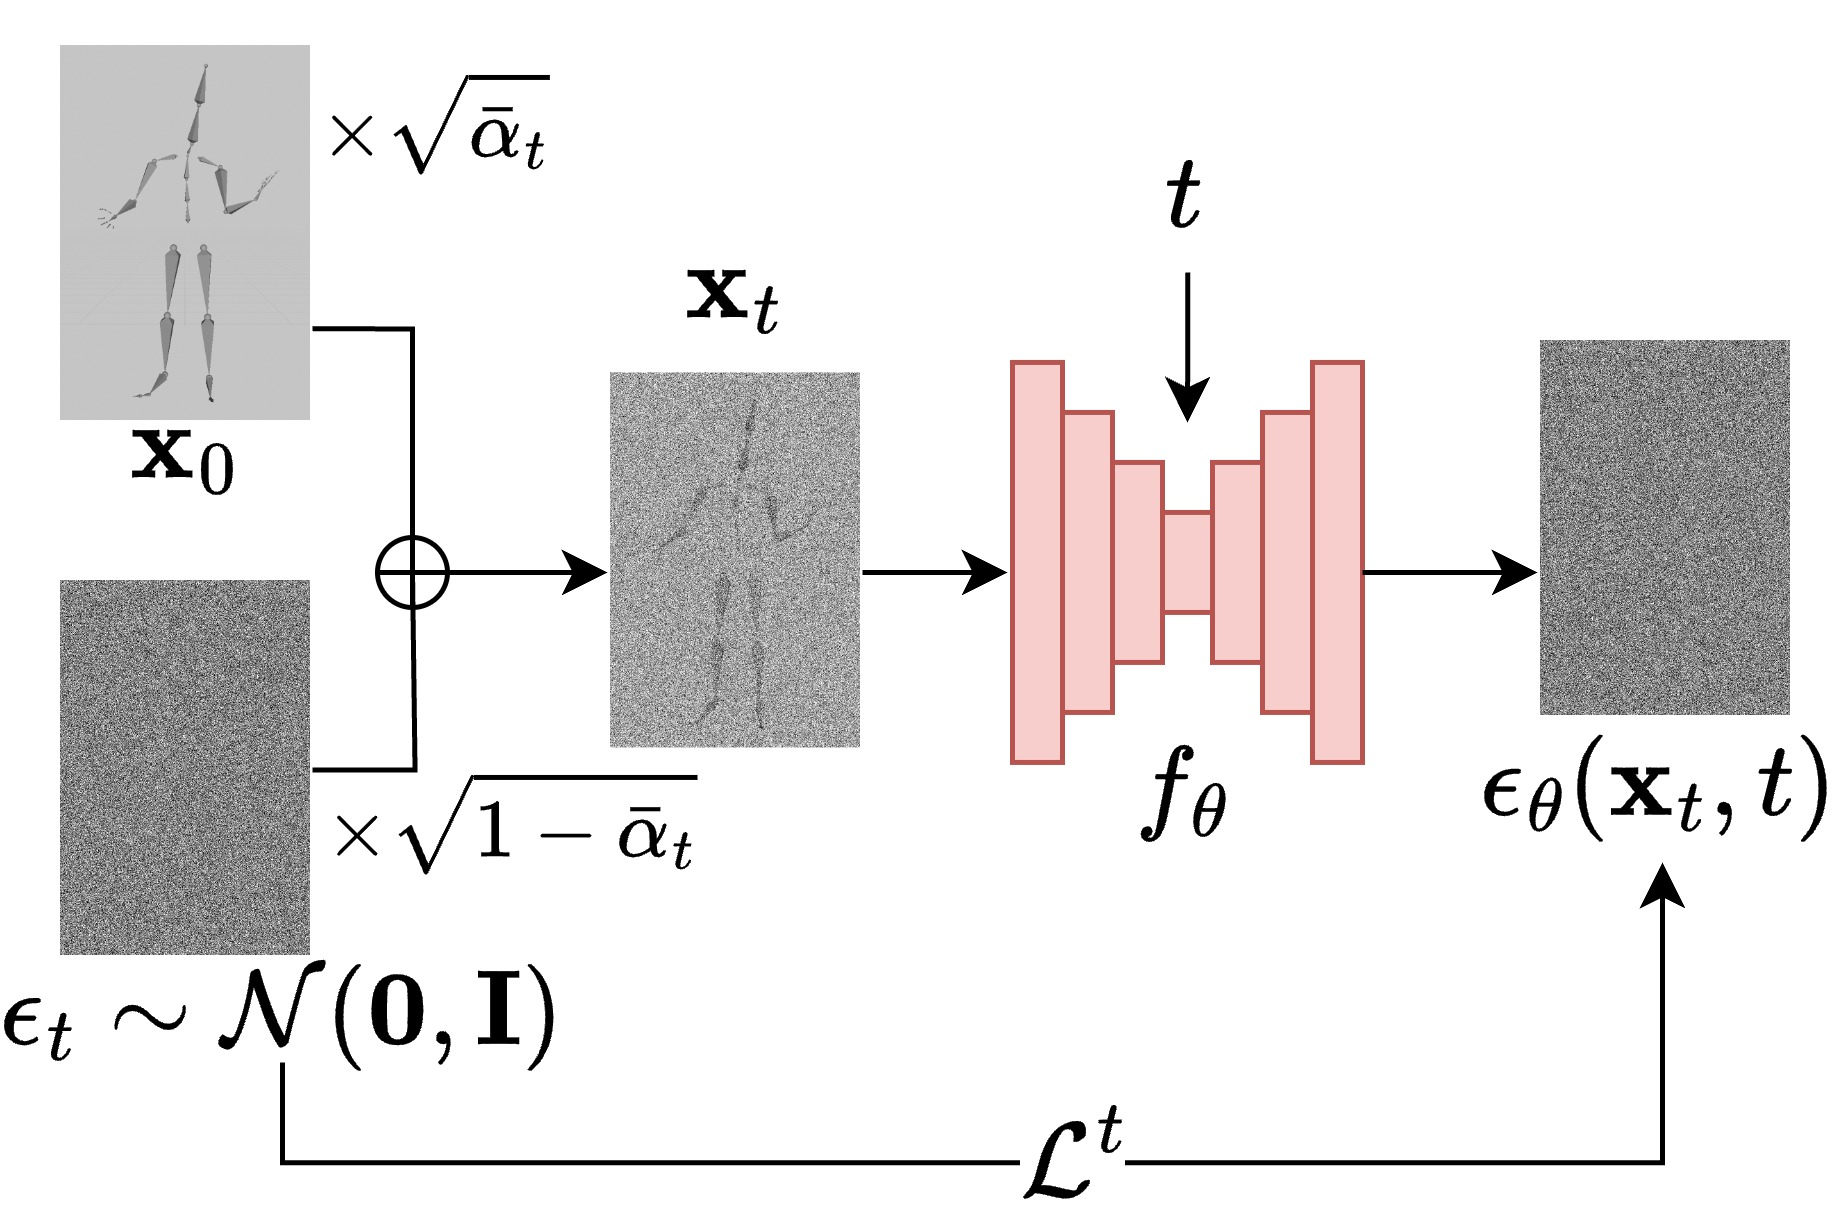
\includegraphics[height=160pt]{AlgorithmForwardDiffusion}
	\caption{Thêm nhiễu trong quá trình huấn luyện}
	\label{fig:AlgorithmForwardDiffusion}
\end{figure}

Vì nhiễu $\boldsymbol{\epsilon}_{t-1}, \boldsymbol{\epsilon}_{t-2}, \dots \sim \mathcal{N}(\mathbf{0}, \mathbf{I})$ luôn luôn là phân phối chuẩn Gaussian, và cho trước trong mọi bước $t$, nên ta có thể dễ dàng truy ngược được $\bx_t$ từ $\bx_0$. Bằng cách đặt $\alpha_t = 1 - \beta_t$ và $\bar{\alpha}_t = \prod_{i=1}^t \alpha_i$, từ \autoref{eq:addgaussian}, ta có hàm forward diffusion viết lại theo $\alpha$ như sau:

%\begin{equation}
%%	\label{eq:tracexzero}
%	\begin{aligned}
%		\mathbf{x}_t 
%		&= \sqrt{\alpha_t}\mathbf{x}_{t-1} + \sqrt{1 - \alpha_t}\boldsymbol{\epsilon}_{t-1} \\
%		&= \sqrt{\alpha_t \alpha_{t-1}} \mathbf{x}_{t-2} + \sqrt{1 - \alpha_t \alpha_{t-1}} \bar{\boldsymbol{\epsilon}}_{t-2}
%		&= \sqrt{\bar{\alpha}_t}\mathbf{x}_0 + \sqrt{1 - \bar{\alpha}_t}\boldsymbol{\epsilon} \\
%		q(\mathbf{x}_t \vert \mathbf{x}_0) &= \mathcal{N}(\mathbf{x}_t; \sqrt{\bar{\alpha}_t} \mathbf{x}_0, (1 - \bar{\alpha}_t)\mathbf{I})
%	\end{aligned}
%\end{equation}

\begin{equation}
\begin{aligned}
	\boldsymbol{x}_t &= \sqrt{\alpha_t}\boldsymbol{x}_{t-1} + \sqrt{1 - \alpha_t}\boldsymbol{\epsilon}_{t-1} \\
	&= \sqrt{\alpha_t}\left(\sqrt{\alpha_{t-1}}\boldsymbol{x}_{t-2} + \sqrt{1 - \alpha_{t-1}}\boldsymbol{\epsilon}_{t-2}\right) + \sqrt{1 - \alpha_t}\boldsymbol{\epsilon}_{t-1} \\
	&= \sqrt{\alpha_t\alpha_{t-1}}\boldsymbol{x}_{t-2} + \sqrt{\alpha_t(1 - \alpha_{t-1})}\boldsymbol{\epsilon}_{t-2} + \sqrt{1 - \alpha_t}\boldsymbol{\epsilon}_{t-1} \\
	&= \sqrt{\alpha_t\alpha_{t-1}}\boldsymbol{x}_{t-2} + \sqrt{\alpha_t(1 - \alpha_{t-1}) + (1 - \alpha_t)}\boldsymbol{\epsilon}_{t-2} \\
	&= \sqrt{\alpha_t\alpha_{t-1}}\boldsymbol{x}_{t-2} + \sqrt{1 - \alpha_t\alpha_{t-1}}\boldsymbol{\epsilon}_{t-2} \\
	&= \ldots \\
	&= \sqrt{\prod_{i=1}^t \alpha_i} \boldsymbol{x}_0 + \sqrt{1 - \prod_{i=1}^t \alpha_i} \boldsymbol{\epsilon}_0 \\
	&= \sqrt{\bar{\alpha}_t} \boldsymbol{x}_0 + \sqrt{1 - \bar{\alpha}_t} \boldsymbol{\epsilon}_0 \\
	&\sim \mathcal{N}\left(\boldsymbol{x}_t; \sqrt{\bar{\alpha}_t} \boldsymbol{x}_0, \left(1 - \bar{\alpha}_t\right) \textbf{I}\right)
\end{aligned}
\label{eq:tracexzero}
\end{equation}

Sự thay đổi của $\sqrt{\alpha}$ và  $\sqrt{1- \alpha}$ trong quá trình gây nhiễu được thể hiện ở phụ lục \autoref{appendix:Appendix1}

\subsection{Quá trình khử nhiễu (denoising process)}
\label{subsection:denoising_process}

\begin{figure}[H]
	\centering
	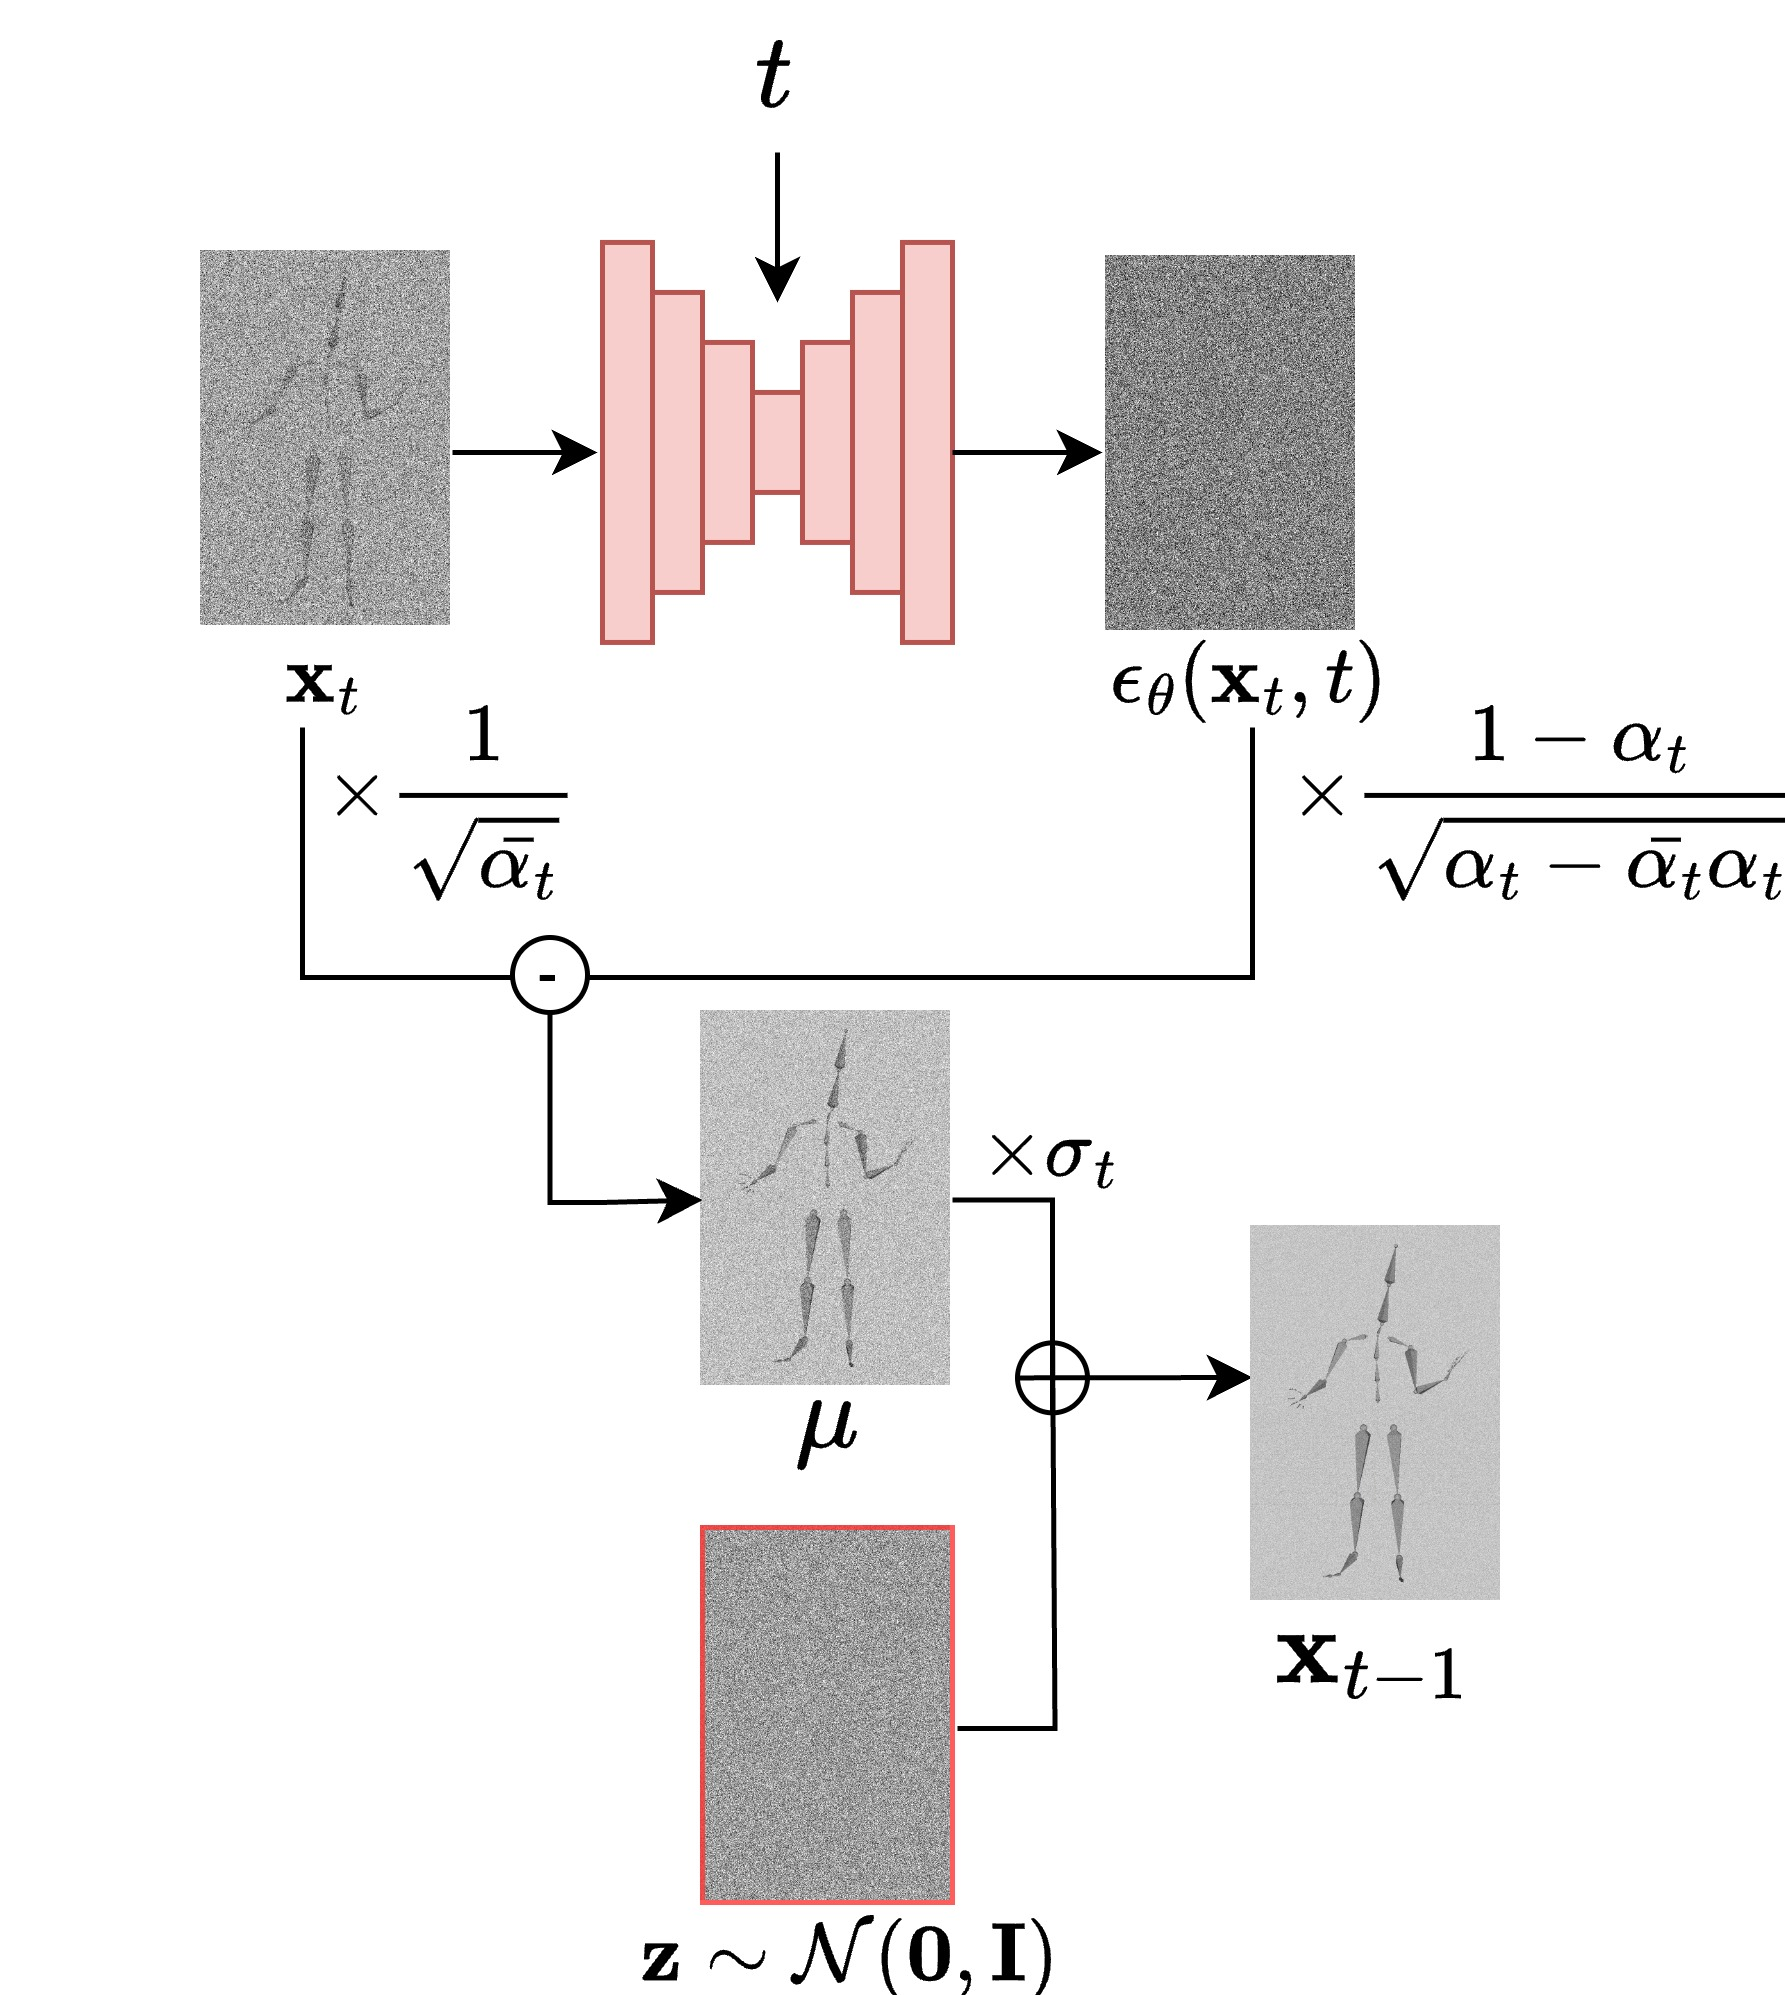
\includegraphics[height=280pt]{AlgorithmSamplingDiffusion}
	\caption{Khử nhiễu trong quá trình suy luận}
	\label{fig:AlgorithmSamplingDiffusion}
	\vspace{-5pt}
\end{figure}

Quá trình khử nhiễu $p_\theta(\mathbf{x}_{t-1} \vert \mathbf{x}_t)$  ở bước thứ $t$ từ $T \to 1$ được bắt đầu từ $\bx_T$ là hoàn toàn nhiễu $\mathcal{N} (\mathbf{0}, \mathbf{I})$. Ta sẽ dùng một neural network $f_{\theta} (\bx_t, t)$ để dự đoán nhiễu $\hat{\epsilon}_t = f_{\theta}(\bx_t, t)$ đã được thêm vào để được $\bx_{t-1}$ từ $\bx_t$.

Quá trình khử nhiễu có trung bình $\boldsymbol{\mu}_\theta(\mathbf{x}_t, t) = {\frac{1}{\sqrt{\alpha_t}} \Big( \mathbf{x}_t - \frac{1 - \alpha_t}{\sqrt{1 - \bar{\alpha}_t}}  f_\theta(\mathbf{x}_t, t) \Big)}$ và phương sai $\boldsymbol{\Sigma}_\theta(\mathbf{x}_t, t)$ như sau:


%\begin{equation} \mathrm{d}\mathbf{x} = [\mathbf{f}(\mathbf{x}, t) - g^2(t) \nabla_\mathbf{x} \log p_t(\mathbf{x})]\mathrm{d}t + g(t) \mathrm{d} \mathbf{w}.\label{rsde} \end{equation}

% bằng cách lấy ảnh bị nhiễu trừ đi nhiễu dự đoán

\begin{equation}
	\label{eq:denoising_process}
	\begin{aligned}
		p_\theta(\mathbf{x}_{0:T})
		&= p(\mathbf{x}_T) \prod^T_{t=1} p_\theta(\mathbf{x}_{t-1} \vert \mathbf{x}_t) \\
		p_\theta(\mathbf{x}_{t-1} \vert \mathbf{x}_t) &= \mathcal{N}(\mathbf{x}_{t-1};  \boldsymbol{\mu}_\theta(\mathbf{x}_t, t), \boldsymbol{\Sigma}_\theta(\mathbf{x}_t, t))
	\end{aligned}
\end{equation}

Qúa trình khử nhiễu là quá trình bắt đầu từ nhiễu hoàn toàn, dùng một neuron network $f_\theta$ để học được quá trình khử nhiễu.

%Ta viết lại hàm denoising từ công thức \ref{eq:denoising_process}  theo $\alpha$ như sau:
%$$
%x_{t-1} = \frac{1}{\sqrt{\alpha_t}} \left( x_t - \frac{\sqrt{1 - \alpha_t}}{\sqrt{1 - \bar{\alpha}_t}} \epsilon_{\theta}(x_t, t) \right) + \sqrt{1 - \alpha_t} \tilde{\epsilon}_t
%$$


%\begin{equation}
%	\label{eq:denoising_alpha}
%	\begin{aligned}
	%	p_\theta(\mathbf{x}_{t-1} \vert \mathbf{x}_t) &= \mathcal{N}(\mathbf{x}_{t-1}; \boldsymbol{\mu}_\theta(\mathbf{x}_t, t), \boldsymbol{\Sigma}_\theta(\mathbf{x}_t, t))
	%\end{aligned} \\
	% \bar{\boldsymbol{\mu}}_t (x_t, t) = \frac{1}{\sqrt{\alpha_t}} \Big( \mathbf{x}_t - \frac{1 - \alpha_t}{\sqrt{1 - \bar{\alpha}_t}} \boldsymbol{\epsilon}_t \Big)
	%\end{equation}
%\subsection{Hàm mất mát trong }


\subsection{Quá trình huấn luyện trong mô hình diffusion cơ bản}
%	Hàm mất mát $\mathcal{L}$ của mô hình diffusion
	
	\begin{figure}[H]
		\centering
		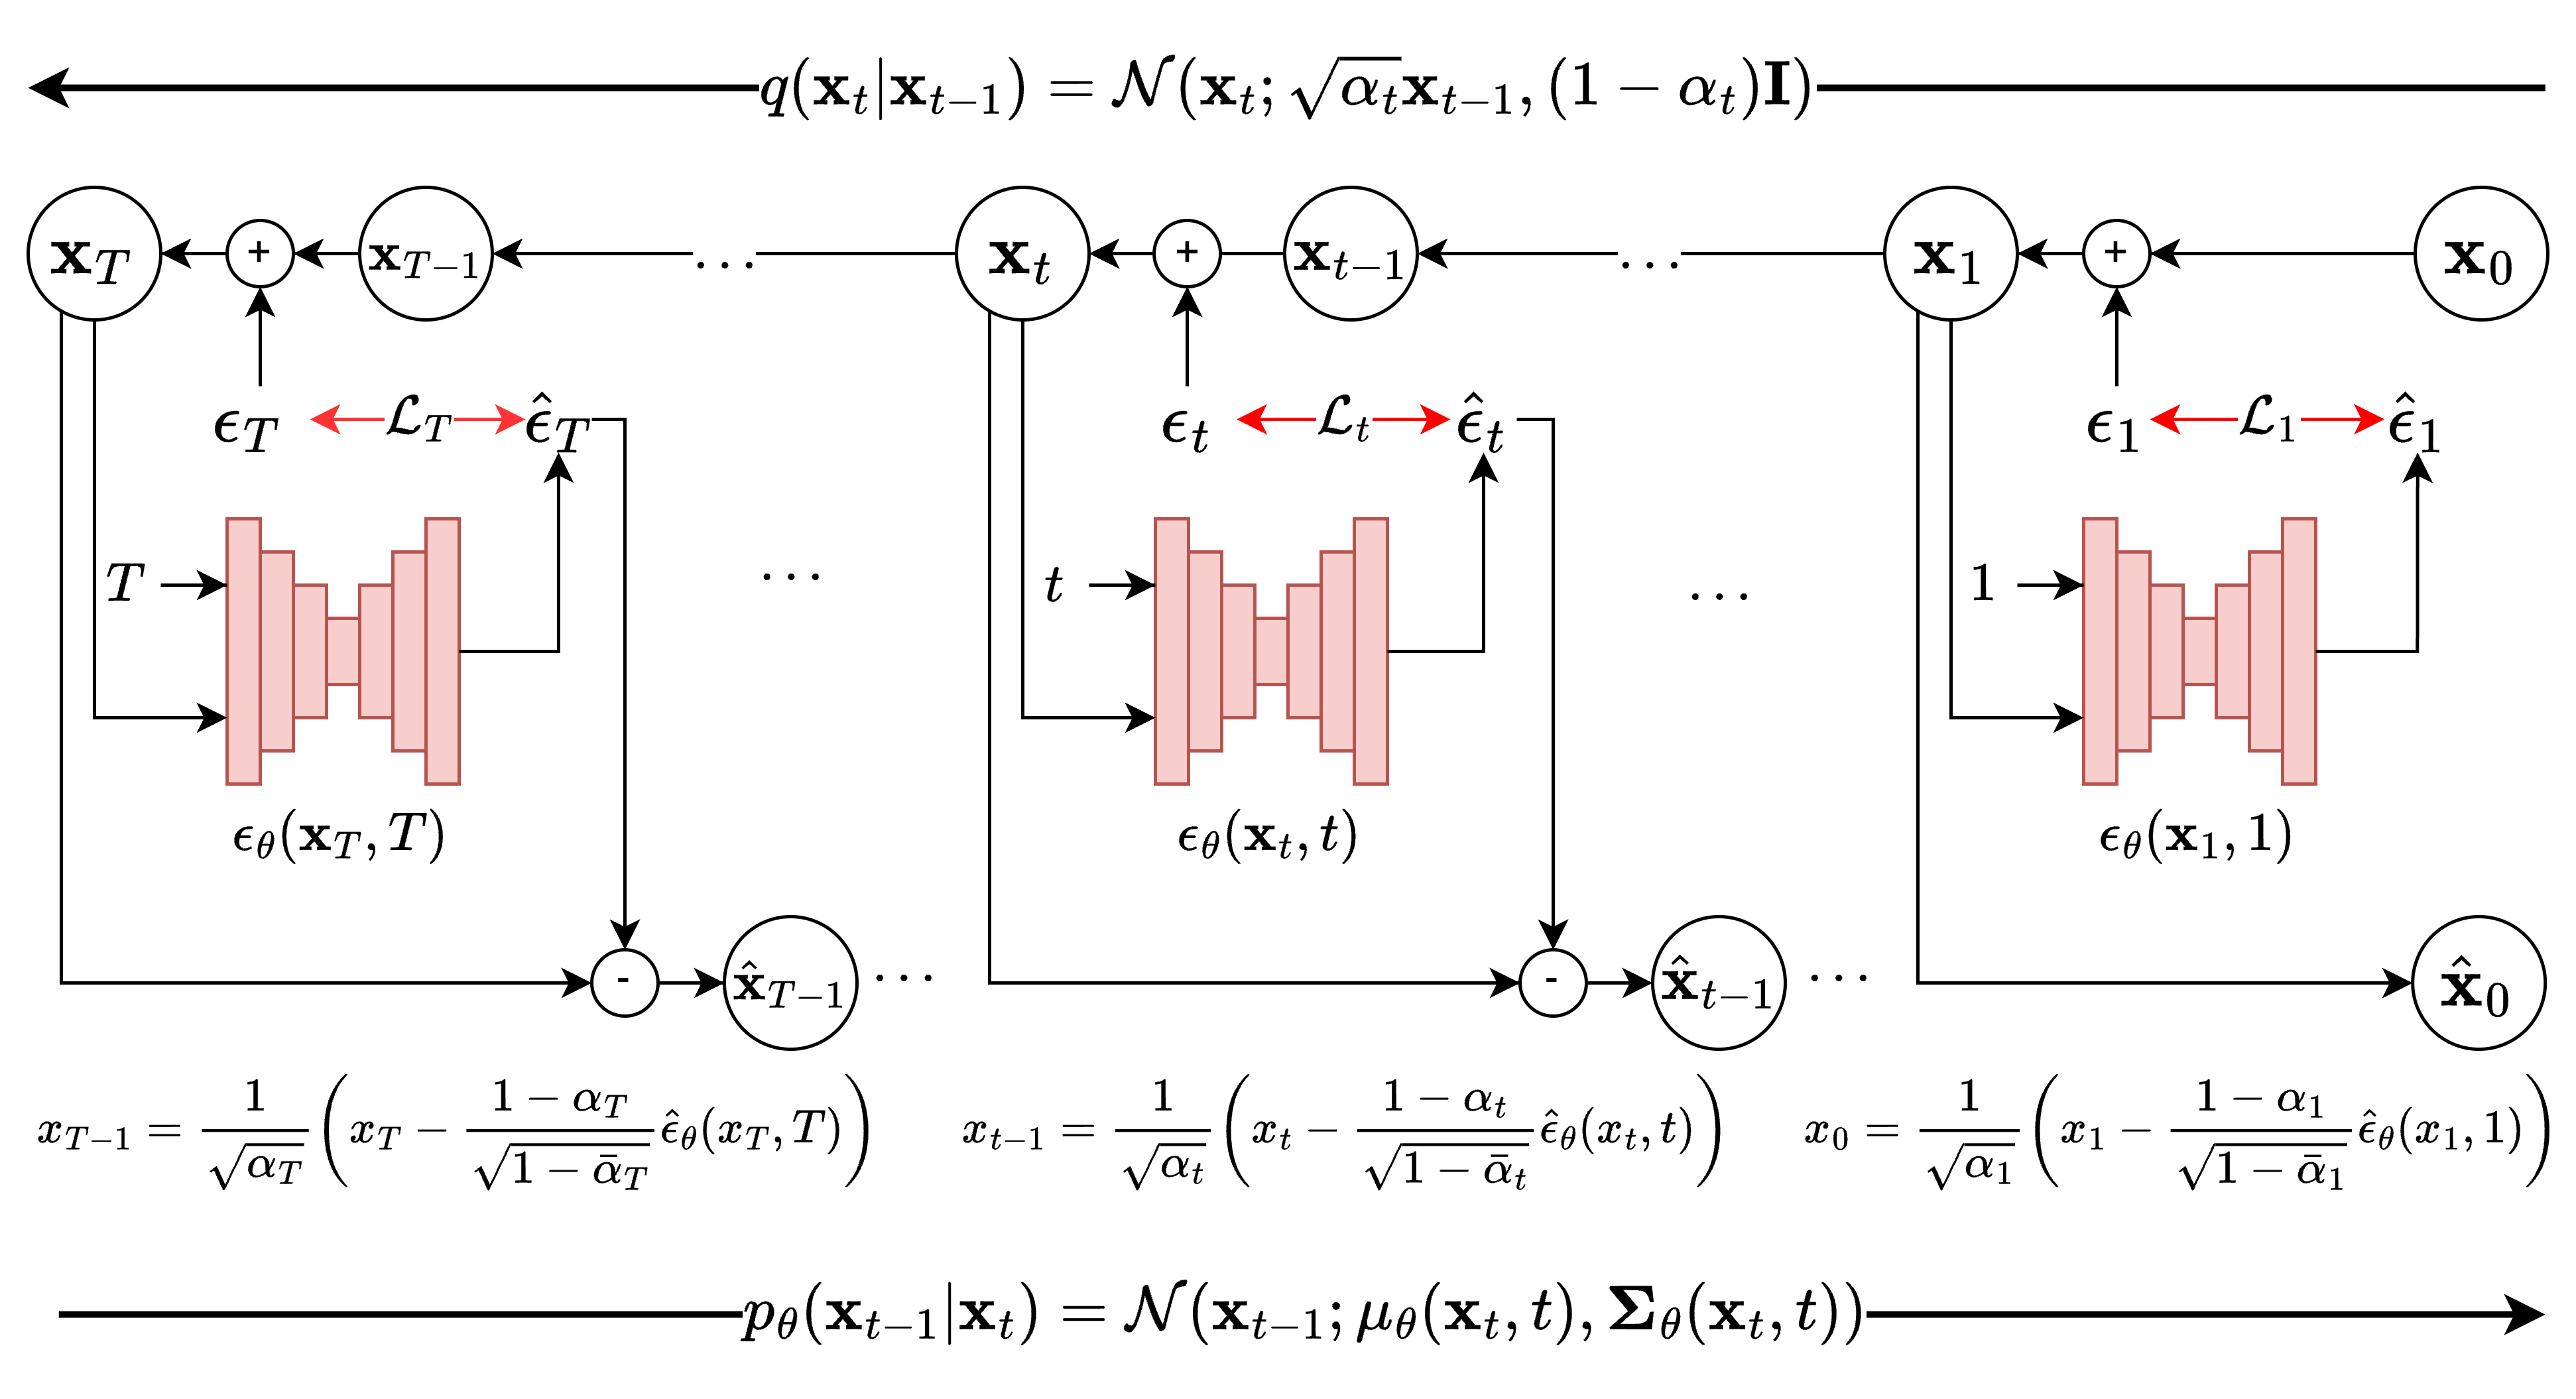
\includegraphics[width=\linewidth]{DDPMTraining}
		\caption{Mô hình diffusion cơ bản}
		\label{fig:basic_diffusion}\
		\vspace{-5pt}
	\end{figure}
	
	Mô hình diffusion sẽ học trọng số $\theta$ của hàm dự đoán lỗi $f_{\theta} (x_t, t)$ hay còn ký hiệu là  $\epsilon_{\theta} (x_t, t)$. Trong quá trình denoising, ta sẽ tối ưu độ lỗi giữa nhiễu dự đoán $\boldsymbol{\epsilon}_\theta(\mathbf{x}_t, t)$ và nhiễu thực tế $\boldsymbol{\epsilon}_t$. Với mỗi bước thứ $t$ ta sẽ tối ưu hàm loss $\mathcal{L}_{t}$ để thu được trọng số $\theta$.
	
	\begin{equation}
		\label{eq:diffusion_loss}
		\begin{aligned}
			\mathcal{L}_t
			&= \mathbb{E}_{t \sim [1, T], \mathbf{x}_0, \boldsymbol{\epsilon}_t} \Big[\|\boldsymbol{\epsilon}_t - \boldsymbol{\epsilon}_\theta(\mathbf{x}_t, t)\|^2 \Big] \\
			&= \mathbb{E}_{t \sim [1, T], \mathbf{x}_0, \boldsymbol{\epsilon}_t} \Big[\|\boldsymbol{\epsilon}_t - \boldsymbol{\epsilon}_\theta(\sqrt{\bar{\alpha}_t}\mathbf{x}_0 + \sqrt{1 - \bar{\alpha}_t}\boldsymbol{\epsilon}_t, t)\|^2 \Big]
		\end{aligned}
	\end{equation}


Trong đó, hàm mất mát $\mathcal{L}$ tổng sẽ là  $\mathcal{L} = \sum_{t=1}^{T} \mathcal{L}_t$.

Với $f_{\theta}(x_{t-1}, t)$ hay $\epsilon_\theta$ là một mô hình Unet dùng để mã hoá và giải mã dữ liệu để dự đoán nhiễu đã thêm vào dữ liệu. Quá trình tính toán hàm lỗi được trình bày minh hoạ trong \autoref{fig:basic_diffusion}.


\begin{algorithm}[H]
	
	\setlength{\baselineskip}{10pt}
	\begin{enumerate}
		\vspace{5pt}
		\item Tính sẵn các giá trị $\sqrt{\alpha_t}$, $\sqrt{1 - \alpha_t}$ và $\sqrt{\bar{\alpha}_t}$ cho mỗi bước $t: 1 \rightarrow T$. Xác định lịch trình nhiễu $\{\alpha_t \in (0, 1)\}_{t=1}^T$, với $\alpha_1 < \alpha_2 < \dots < \alpha_T$.
		
		\item Lấy nhãn $\mathbf{x}_0$ từ phân phối của dữ liệu đã chuẩn hoá.
		
		\item Tạo nhiễu ngẫu nhiên $\boldsymbol{\epsilon}_t$ cho mỗi bước $t: 1 \rightarrow T$, với $\forall t: \boldsymbol{\epsilon}_t \sim \mathcal{N}(\mathbf{0}, \mathbf{I})$.
		
		\item Gây nhiễu (forward) $\mathbf{x}_0$ để thu được $\mathbf{x}_t$ ở mỗi bước $t: 1 \rightarrow T$:
		$$
		\mathbf{x}_t = \sqrt{\bar{\alpha}_t} \mathbf{x}_0 + \sqrt{1 - \bar{\alpha}_t} \boldsymbol{\epsilon}_t
		$$
		
		\item Với mỗi $t$, lấy $t$ \textbf{ngẫu nhiên} từ $[1, T]$.
		
		\item Cho $\mathbf{x}_t$ và $t$ vào mô hình để dự đoán nhiễu: $\hat{\boldsymbol{\epsilon}} = \boldsymbol{\epsilon}_\theta(\mathbf{x}_t, t)$.
		
		\item Tính đạo hàm để cập nhật trọng số:
		$$
		\grad_{\theta_t} \left\| \boldsymbol{\epsilon}_t - \boldsymbol{\epsilon}_\theta(\mathbf{x}_t, t) \right\|^2
		$$
		Tính loss:
		$$
		\mathcal{L}_t = \mathbb{E}_{t \sim [1, T], \mathbf{x}_0, \boldsymbol{\epsilon}_t} \left[ \|\boldsymbol{\epsilon}_t - \boldsymbol{\epsilon}_\theta(\sqrt{\bar{\alpha}_t} \mathbf{x}_0 + \sqrt{1 - \bar{\alpha}_t} \boldsymbol{\epsilon}_t, t)\|^2 \right]
		$$
		
		\item Quay lại bước 6 cho đến khi hội tụ để thu được trọng số tối ưu $\theta'$.
	\end{enumerate}
	\caption{Thuật toán training trong DDPM}
	\label{alg:TrainingDDPM}
\end{algorithm}

%	Lưu ý 
%	Thay vì dùng neuron network để dự đoán phân bố của dữ liệu theo như hình \ref{fig:basic_diffusion}, mô hình diffusion sẽ dự đoán độ lỗi được thêm vào trong ảnh ở bước thứ $t$, với mỗi $t$ bước ta sẽ cần tối ưu hàm mất mát $\mathcal{L}_t$, hàm mất mát của mỗi bước sẽ tối ưu độ lỗi giữa nhiễu dự đoán $\hat{\epsilon_t}$ và nhiễu nhãn $\epsilon_t$ được thêm vào.
	
\subsection{Quá trình lấy mẫu trong diffusion cơ bản}
	
		\begin{figure*}
		\centering
		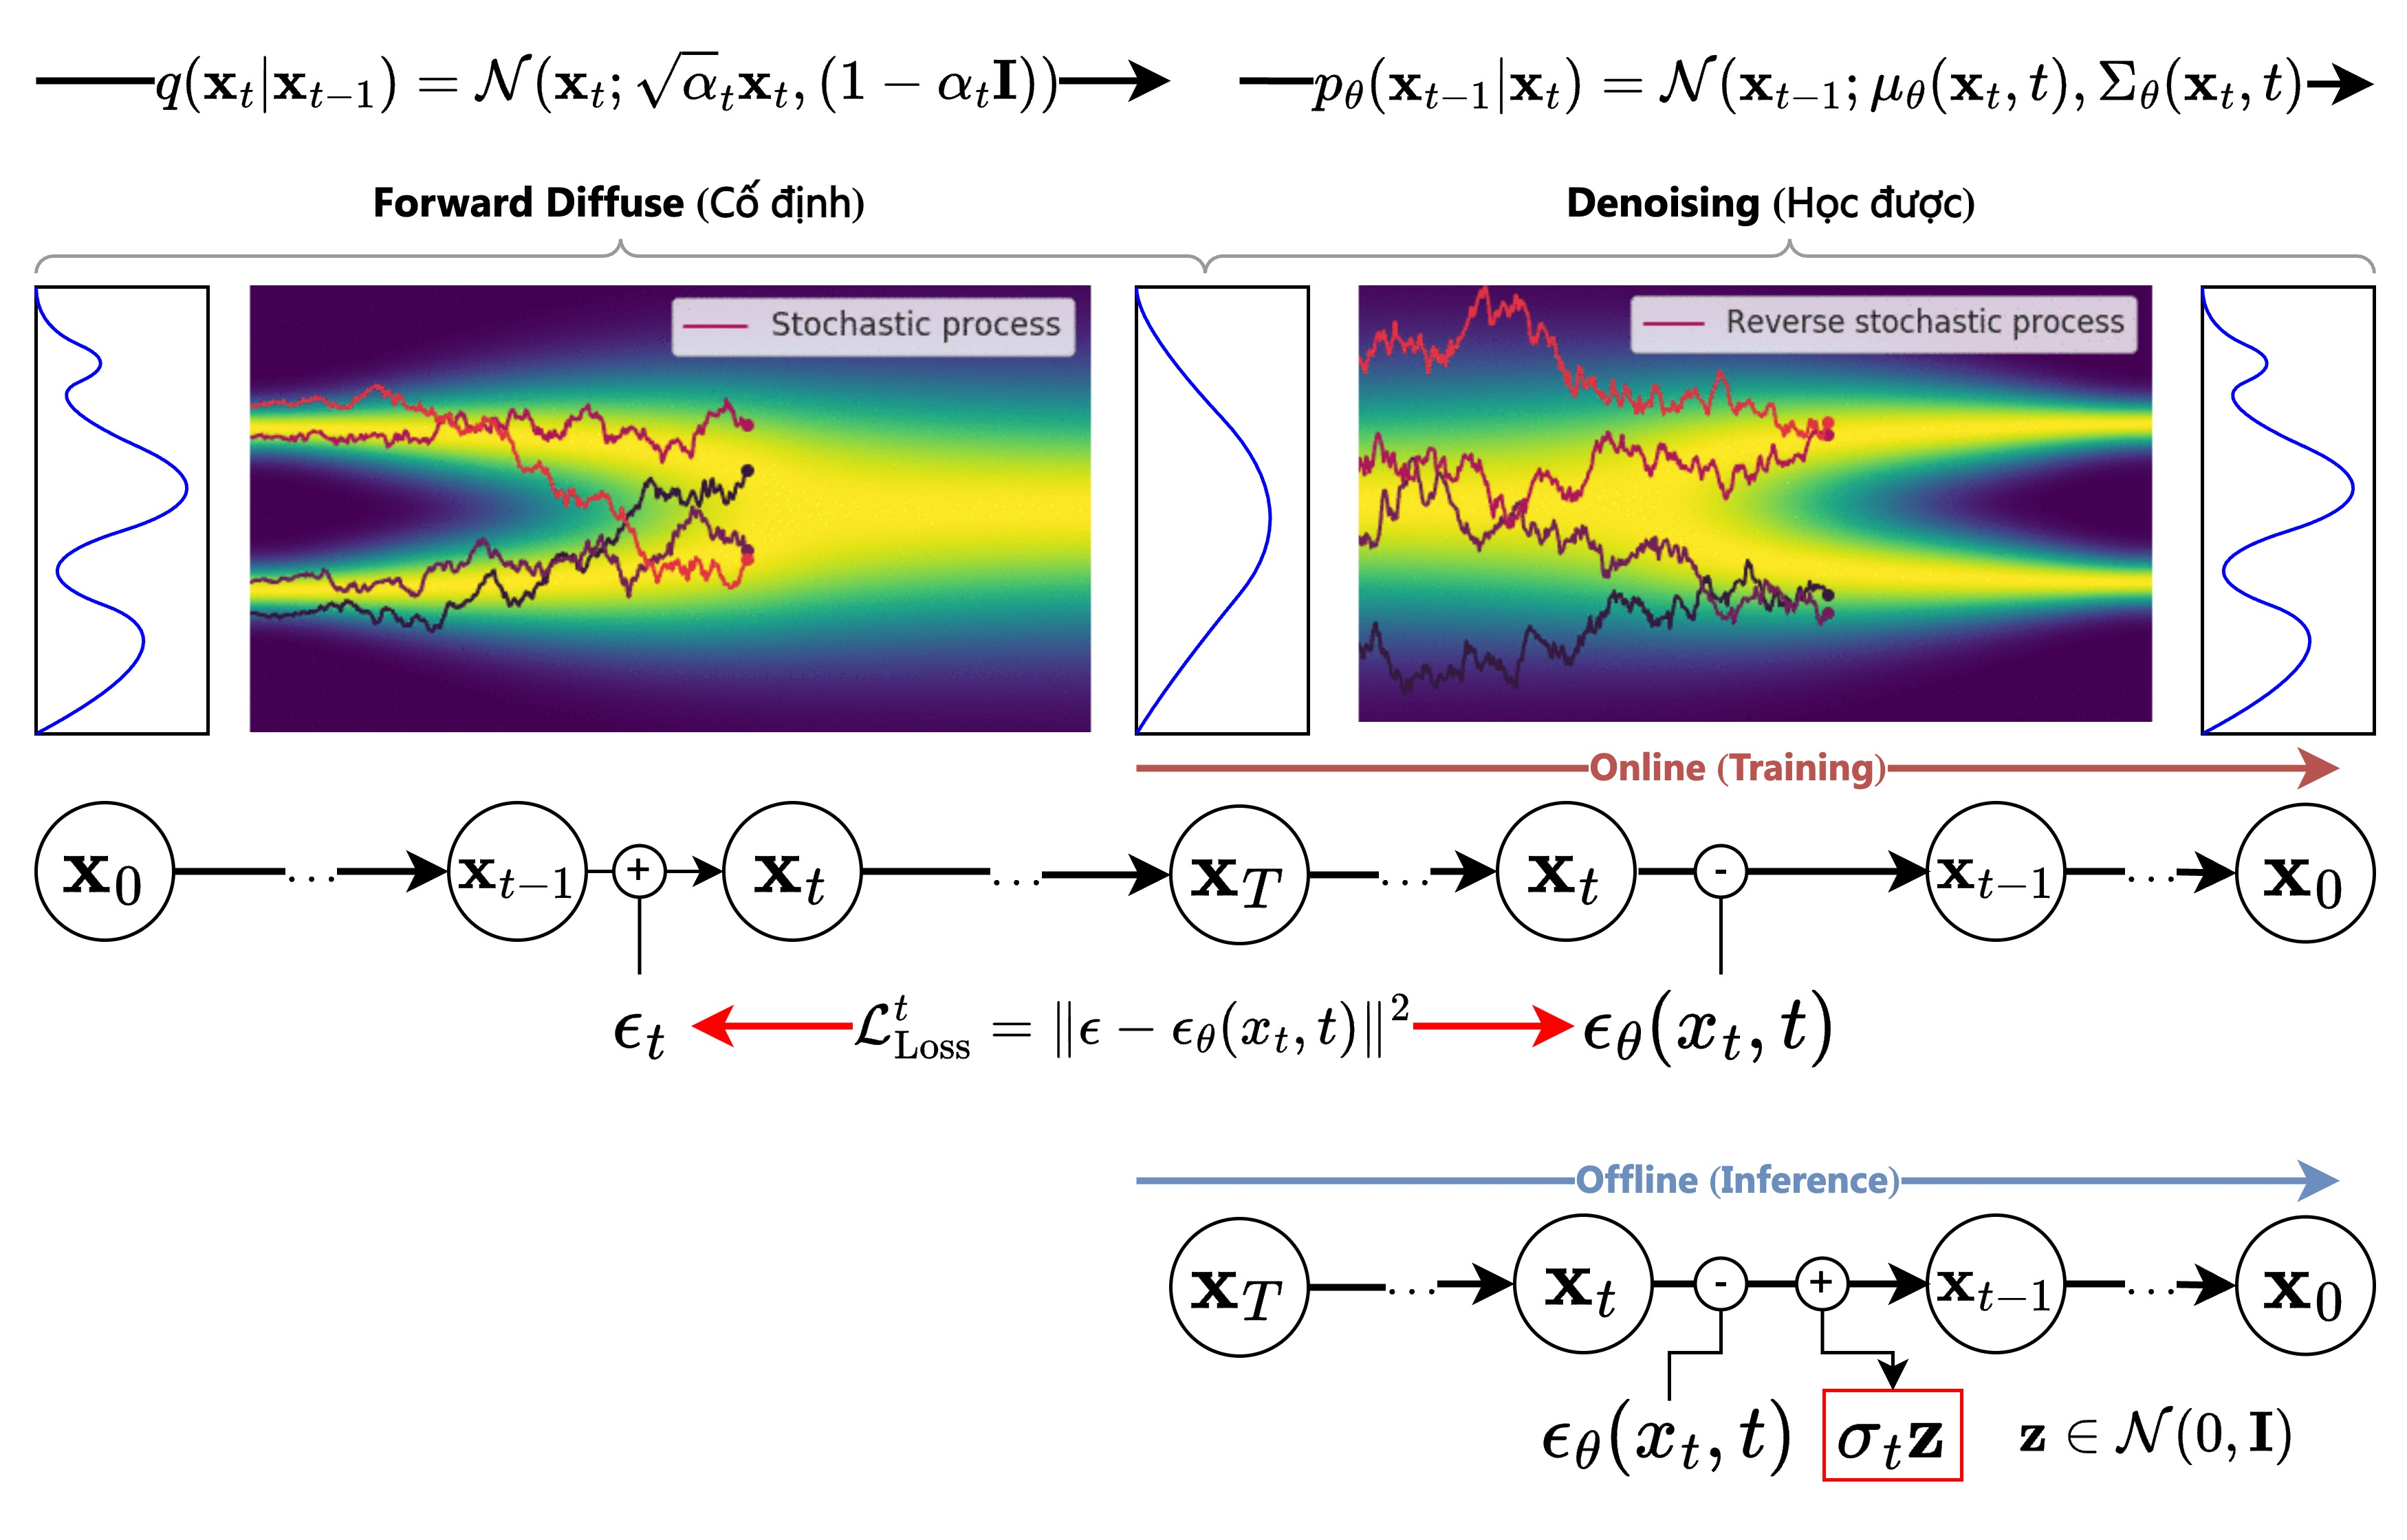
\includegraphics[width=\linewidth]{TrainingAndSamplingStandard}
		\caption{Quá trình Training và Sampling trong mô hình Diffusion tiêu chuẩn}
		\label{fig:GaussianDrift}
	\end{figure*}
	

	Sau khi thu được trọng số $\theta'$, ta sẽ dùng hàm denoising để khử nhiễu từ nhiễu $\bx_T \sim \mathcal{N} (\mathbf{0}, \mathbf{I})$.
	Quá trình biến đổi từ nhiễu hoàn toàn $\bx_{T}$ sang dự đoán $\hat{\bx_0}$ như sau:
	%với $t$ là một vector đã được nhúng vị trí bằng thuật toán nhúng
	
	\begin{equation}
		\label{eq:adddenoising}
	\bx_{t-1} = \frac{1}{\sqrt{\alpha_t}} \left( \bx_t - \frac{1- \alpha_t}{\sqrt{1 - \bar{\alpha}_t}} f_{\theta'}(\bx_t, t) \right) + \sqrt{1 - \alpha_t} \tilde{\epsilon}_t
	\end{equation}
	
Lưu ý rằng $\epsilon_t$ là nhiễu cố định và lấy ngẫu nhiên trước quá trình huấn luyện, chỉ sử dụng lại kết quả ngẫu nhiên trong quá trình forward diffusion \autoref{subsection:denoising_process} ở công thức  \autoref{eq:addgaussian}. Như \autoref{fig:GaussianDrift}, độ lỗi $\epsilon_t$ là độ nhiễu của từng bước $t$, và hàm loss  $\mathcal{L}^{t}$ sẽ tính theo từng bước $t$.


Tiếp theo quá trình huấn luyện, thuật toán lấy mẫu (sampling) trong DDPM bắt đầu từ bước tạo nhiễu hoàn toàn, tức là $\mathbf{x}_T \sim \mathcal{N}(0, \mathbf{I})$, nơi dữ liệu ban đầu hoàn toàn là nhiễu. Các giá trị $\sqrt{\alpha_t}$, $\sqrt{1 - \alpha_t}$ và $\sqrt{\bar{\alpha}_t}$, được tính từ quá trình huấn luyện, sẽ được sử dụng trong quá trình lấy mẫu để dự đoán lại dữ liệu gốc $\mathbf{x}_0$. Bước tiếp theo là tính toán hệ số điều chỉnh nhiễu $\sigma_t$, dựa vào lịch trình nhiễu $\alpha_t$ đã xác định trong quá trình huấn luyện. Các giá trị này sẽ ảnh hưởng đến độ nhiễu được thêm vào trong quá trình lấy mẫu ngược.

Quá trình lấy mẫu (sampling) như \autoref{alg:samplingddpm} sẽ được thực hiện từ bước $T$ trở về $1$, và trong mỗi bước, một nhiễu ngẫu nhiên $\mathbf{z} \sim \mathcal{N}(0, \mathbf{I})$ được tạo ra để cộng thêm vào kết quả dự đoán. Tại mỗi bước $t$, mô hình sẽ dự đoán nhiễu $\boldsymbol{\epsilon}_{\theta'}$ dựa trên dữ liệu nhiễu $\mathbf{x}_t$ và bước thời gian $t$, sau đó sử dụng dự đoán này để tính toán giá trị $\mu$, là ước lượng của $\mathbf{x}_0$. Cuối cùng, một lượng nhiễu $\sigma_t \mathbf{z}$ được cộng thêm vào $\mu$ để thu được $\hat{\mathbf{x}}_{t-1}$, dữ liệu nhiễu tại bước $t-1$. Quá trình này tiếp tục cho đến khi $t = 1$, và khi đó, chúng ta có được $\hat{\mathbf{x}}_0$ — dự đoán cuối cùng của dữ liệu gốc từ quá trình khử nhiễu.

%Mục tiêu của quá trình lấy mẫu này là phục hồi lại dữ liệu ban đầu $\mathbf{x}_0$ từ nhiễu hoàn toàn, đồng thời đảm bảo tính ổn định và sự đa dạng trong quá trình sinh mẫu thông qua việc sử dụng nhiễu ngẫu nhiên $\mathbf{z}$.


\begin{algorithm}[H]
	\caption{Thuật toán sampling trong DDPM}
	\label{alg:samplingddpm}
	\setlength{\baselineskip}{10pt}
	\begin{enumerate}
		\item Bắt đầu với nhiễu: $\mathbf{x}_T \sim \mathcal{N}(0, \mathbf{I})$.
		
		\item Các giá trị $\sqrt{\alpha_t}$, $\sqrt{1 - \alpha_t}$ và $\sqrt{\bar{\alpha}_t}$ được lấy từ quá trình huấn luyện.
		
		\item Tính hệ số điều chỉnh nhiễu $\sigma_t$ từ $\alpha_t$ ở mỗi bước $t: 1 \rightarrow T$:
		\[
		\sigma_t = \sqrt{\frac{1 - \bar{\alpha}_{t-1}}{1 - \bar{\alpha}_t} (1 - \alpha_t)}
		\]
		
		\item Với mỗi $t$, lấy $t$ \textbf{tuần tự} từ $[T, \dots, 1]$.
		
		\item Tạo nhiễu ngẫu nhiên $\mathbf{z} \sim \mathcal{N}(0, \mathbf{I})$.
		
		\item Đưa $\mathbf{x}_t$ vào mô hình để suy luận nhiễu: $\boldsymbol{\epsilon}_{\theta'} = \boldsymbol{\epsilon}_{\theta'}(\mathbf{x}_t, t)$.
		
		\item Dùng nhiễu dự đoán để trừ đi $\mathbf{x}_t$ ở bước $t$:
		\[
		\mu = \frac{1}{\sqrt{\alpha_t}} \left( \mathbf{x}_t - \frac{1 - \alpha_t}{\sqrt{1 - \bar{\alpha}_t}} \boldsymbol{\epsilon}_{\theta'}(\mathbf{x}_t, t) \right)
		\]
		
		\item Cộng thêm một lượng nhiễu: $\hat{\mathbf{x}}_{t-1} = \mu + \sigma_t \mathbf{z}$.
		
		\item Khi $t = 1$, thu được $\hat{\mathbf{x}}_0$ từ quá trình khử nhiễu.
	\end{enumerate}

\end{algorithm}

Điều quan trọng nhất trong quá trình lấy mẫu (denoising sampling) đó chính là phải cộng thêm một độ nhiễu $\mathbf{z} \in \mathcal{N}(0, \mathbf{I})$, với $\mathbf{z}$  sẽ được lần lượt thêm ở từng bước $t$ bằng hệ số điều khiển $\sigma_t$. Mục tiêu của nhiễu $\epsilon$ là để  làm gờ phân phối (marginal noise distribution) cho mô hình $f_\theta$ (hay $\epsilon_{\theta}$) có thể học được nhiễu, còn với  $\mathbf{z}$ là để tăng tính đa dạng trong quá trình sinh và sự ổn định trong quá trình lấy mẫu. Quá trình giảm $\sigma_t$ được trình bày ở phụ lục \autoref{appendix:Appendix1:NoiseScale}


\subsection{Cải tiến mô hình diffusion với dự đoán $\bx_0$ thay vì $\epsilon_t$}
\label{subsec:X0Objective}

Dựa vào \autoref{eq:tracexzero}, có thể thấy nếu có $\bx_{t}$ thì sẽ suy ra được $\bx_0$. Và nếu có $\bx_0$ thì cũng sẽ có thể suy ra được $\bx_{t}$ \textbf{một cách tường minh} với $t$ bất kỳ bằng cách thêm nhiễu $\epsilon_t$ đã có từ quá trình thêm nhiễu thuận (forward diffuse).

Từ quan sát này, nhóm tác giả \cite{nichol2021improved} đề xuất cải tiến DDPM, thay vì dùng hàm neural network $f_{\theta}(\bx_t, t)$ để dự đoán $\epsilon_t$ như \autoref{fig:basic_diffusion} thì $f_{\theta}(\bx_t, t)$ sẽ được dùng để dự đoán trực tiếp $\bx_0$, và khi có $\bx_0$ sẽ thêm nhiễu bằng  \autoref{eq:tracexzero}


\begin{figure}[H]
	\captionsetup{skip=2pt}
	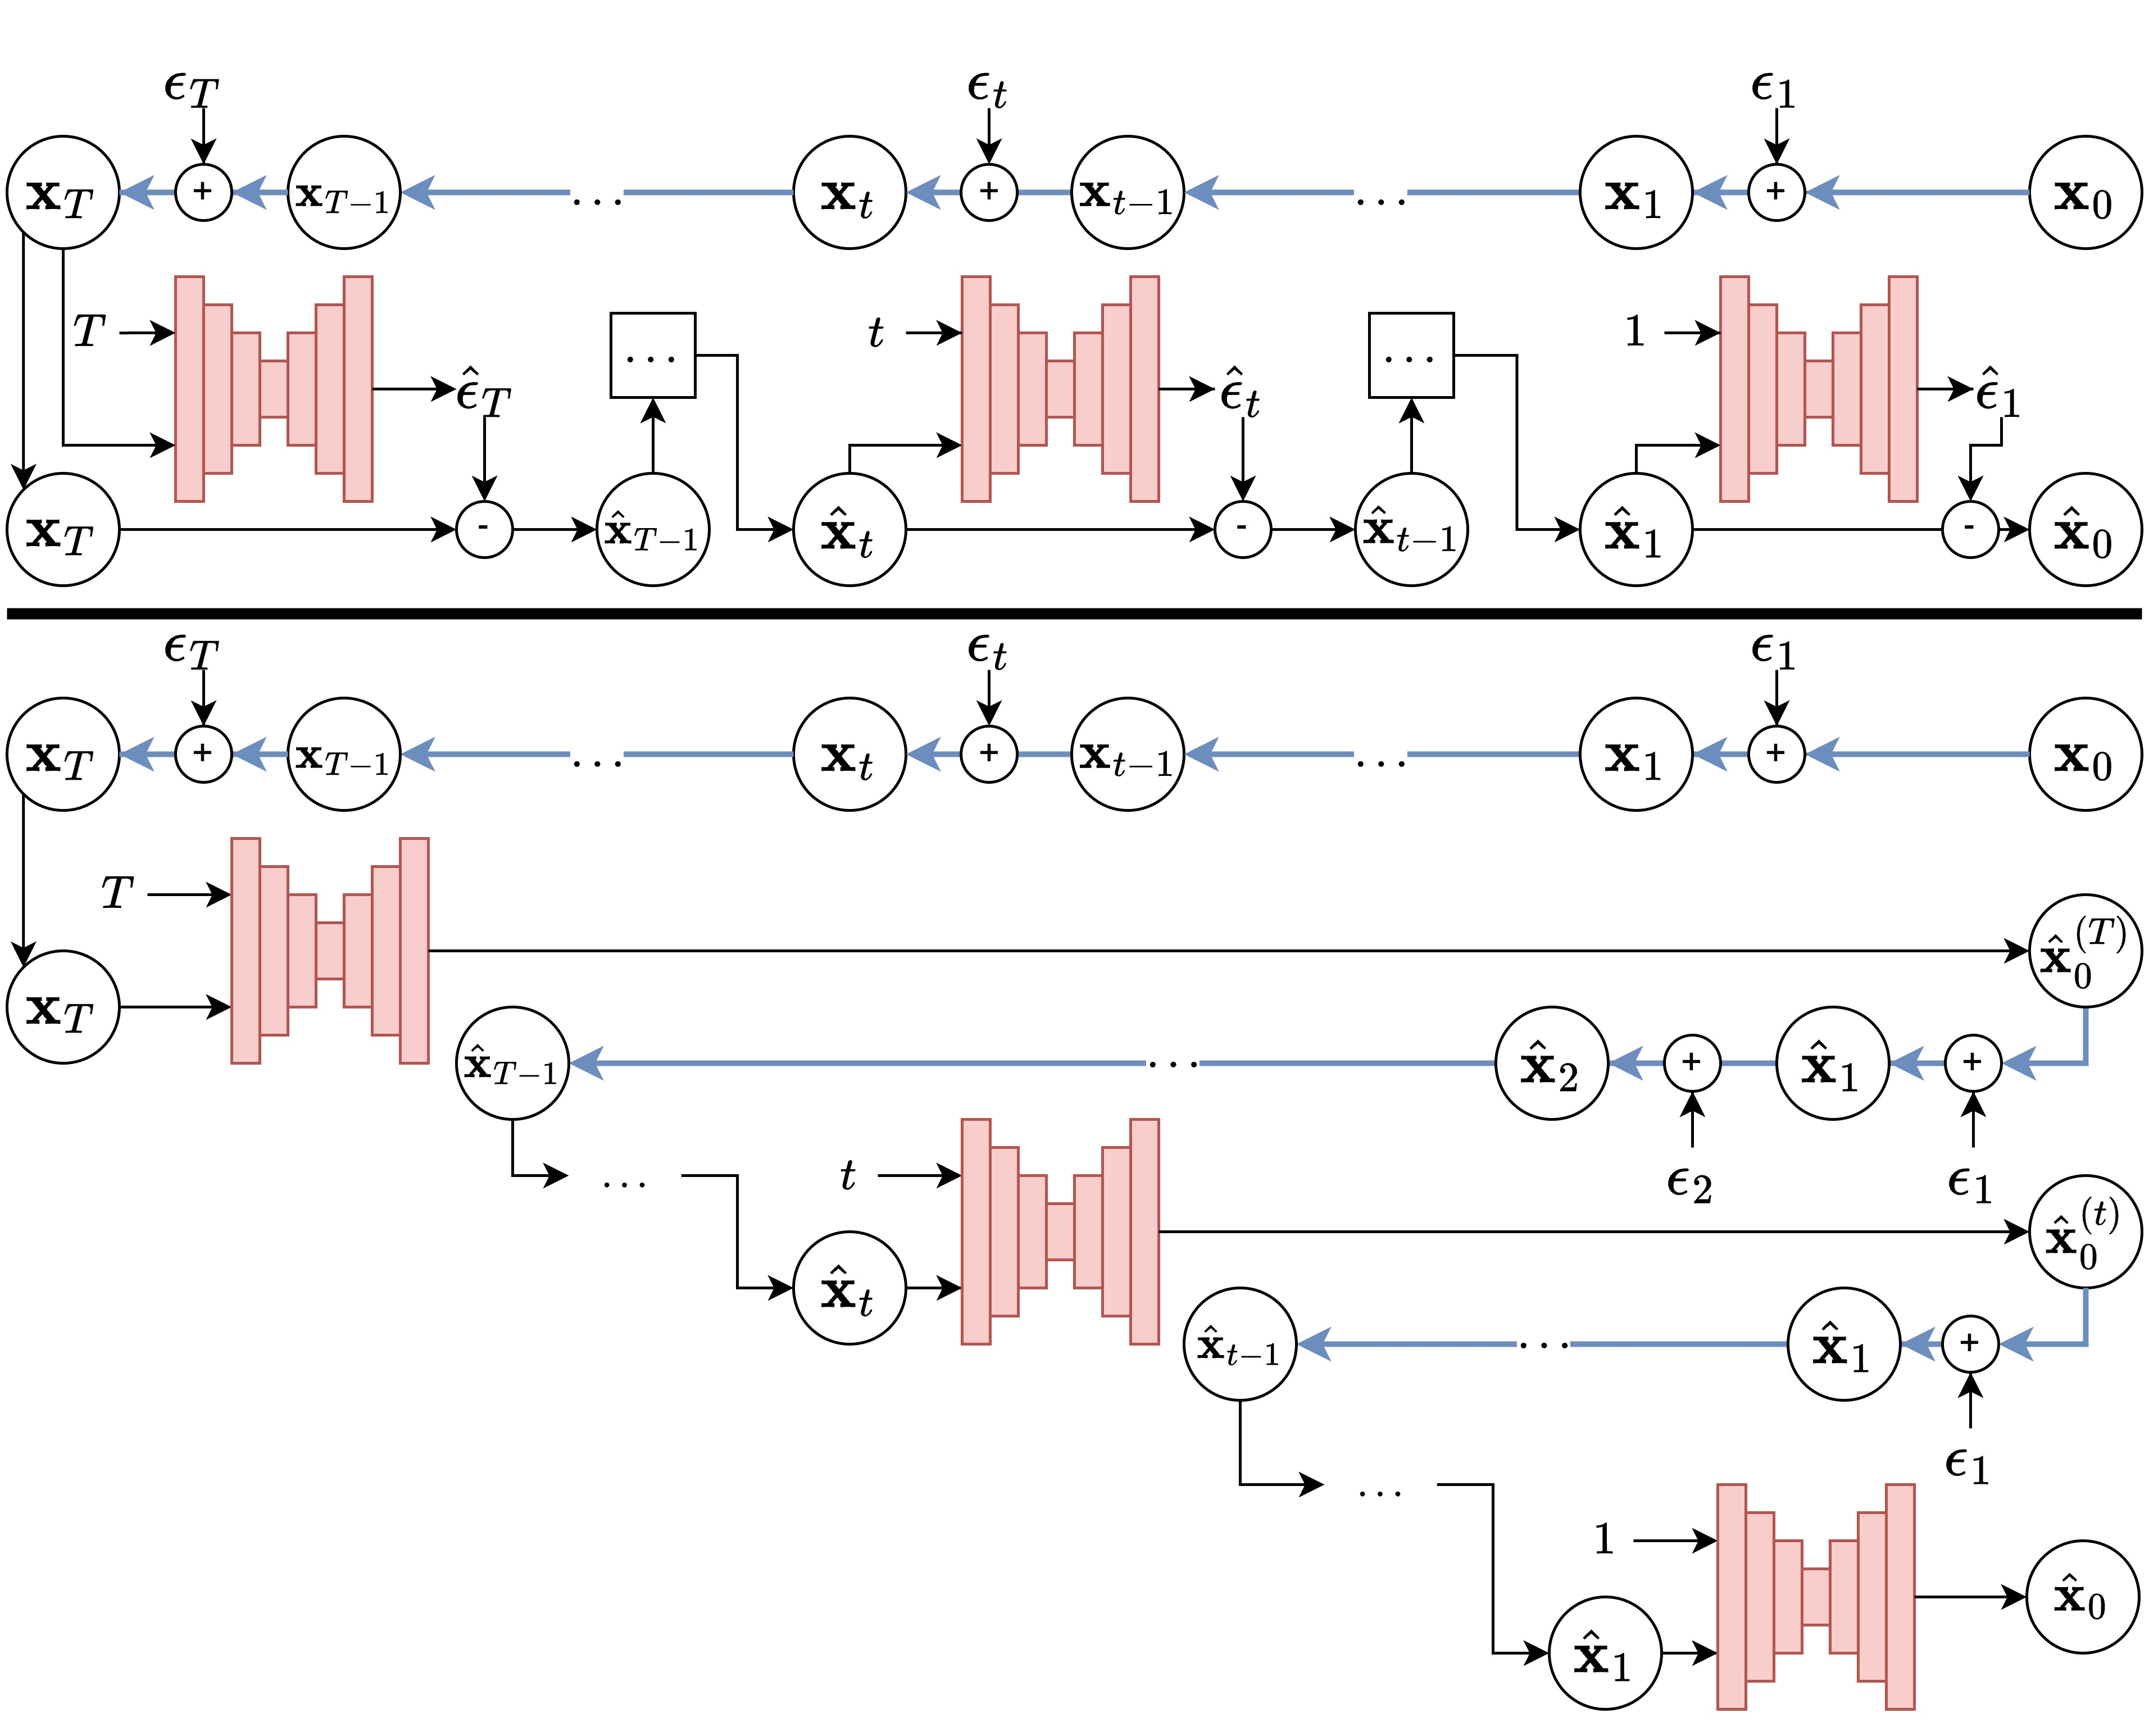
\includegraphics[width=\linewidth]{X0Objective}
	\caption{So sánh $\epsilon$ objective (bên trên) và  $\bx_0$ objective (bên dưới)}
	\label{fig:X0Objective}
\end{figure}

Như hình \autoref{fig:X0Objective}, ta bắt đầu bằng việc thêm nhiễu thuận (forward diffusion), từ $t: 1 \rightarrow T$ để được $\bx_T \sim \mathcal{N} (0, \mathbf{I})$. Sau khi có nhiễu $\bx_{T}$ ta sẽ đưa vào hàm $f_{\theta}$ để dự đoán $\hat{\bx}_0$, từ $\hat{\bx}_0$ sẽ thêm nhiễu để được $\hat{\bx}_{t-1}$. Thực hiện lần lượt đến khi $t = 1$, ta sẽ thu được $\hat{\bx}_0$. Ta có thể so sánh hai phương pháp như sau:

\begin{itemize}
	\item \textbf{$\epsilon$  objective} :  mô hình sẽ dự đoán lỗi. Bắt đầu từ việc forward quá trình gây nhiễu để lấy được $\bx_T$, khi có được $\bx_T$ ta sẽ sử dụng $\bx_T \in \mathcal{N}(0, \mathbf{I})$ để đưa vào quá trình denoise. Trong quá trình denoise, mô hình sẽ dự đoán nhiễu $\hat{\epsilon}_t$ đã được thêm vào từ quá trình forward, là nhiễu $\epsilon_t$ và tối ưu lỗi giữa nhiễu dự đoán và nhiễu thực tế từ quá trình forward.
	\item \textbf{$\bx_0$ objective} : tương tự mô hình sẽ forward quá trình gây nhiễu để lấy được $\bx_T$, khi có được $\bx_T$ ta sẽ sử dụng $\bx_T \in \mathcal{N}(0, \mathbf{I})$ để đưa vào quá trình denoise. Mô hình sẽ dự đoán trực tiếp $\bx_0$, sau khi có $\bx_0$ mô hình sẽ tiếp tục gây nhiễu (Diffuse ) đến bước thứ $\bx_{t-1}$, và tiếp tục sử dụng $\bx_{t-1}$ để đưa vào mô hình dự đoán $\bx_0$
\end{itemize}

\subsection{Mô hình diffusion có điều kiện}
\label{subsec:DiffusionCondition}

Để có thể điều khiển quá trình sinh với các điều kiện khác nhau, thì cần phải sinh với điều kiện $c$, hay nói cách khác ta cần tìm xác xuất $p(\bx | c)$ khi biết trước $c$. Nhóm tác giả \cite{dhariwal2021diffusion} đề xuất sử dụng một hàm $f_{\phi}$ riêng để huấn luyện cho điều kiện. Tuy nhiên phương pháp này gây khó khăn khi các điều kiện sinh thay đổi và việc kết hợp và cập nhật trọng số ở một mô hình riêng sẽ gây khó khăn khi mở rộng.

\begin{figure}[H]
	\captionsetup{skip=20pt}
	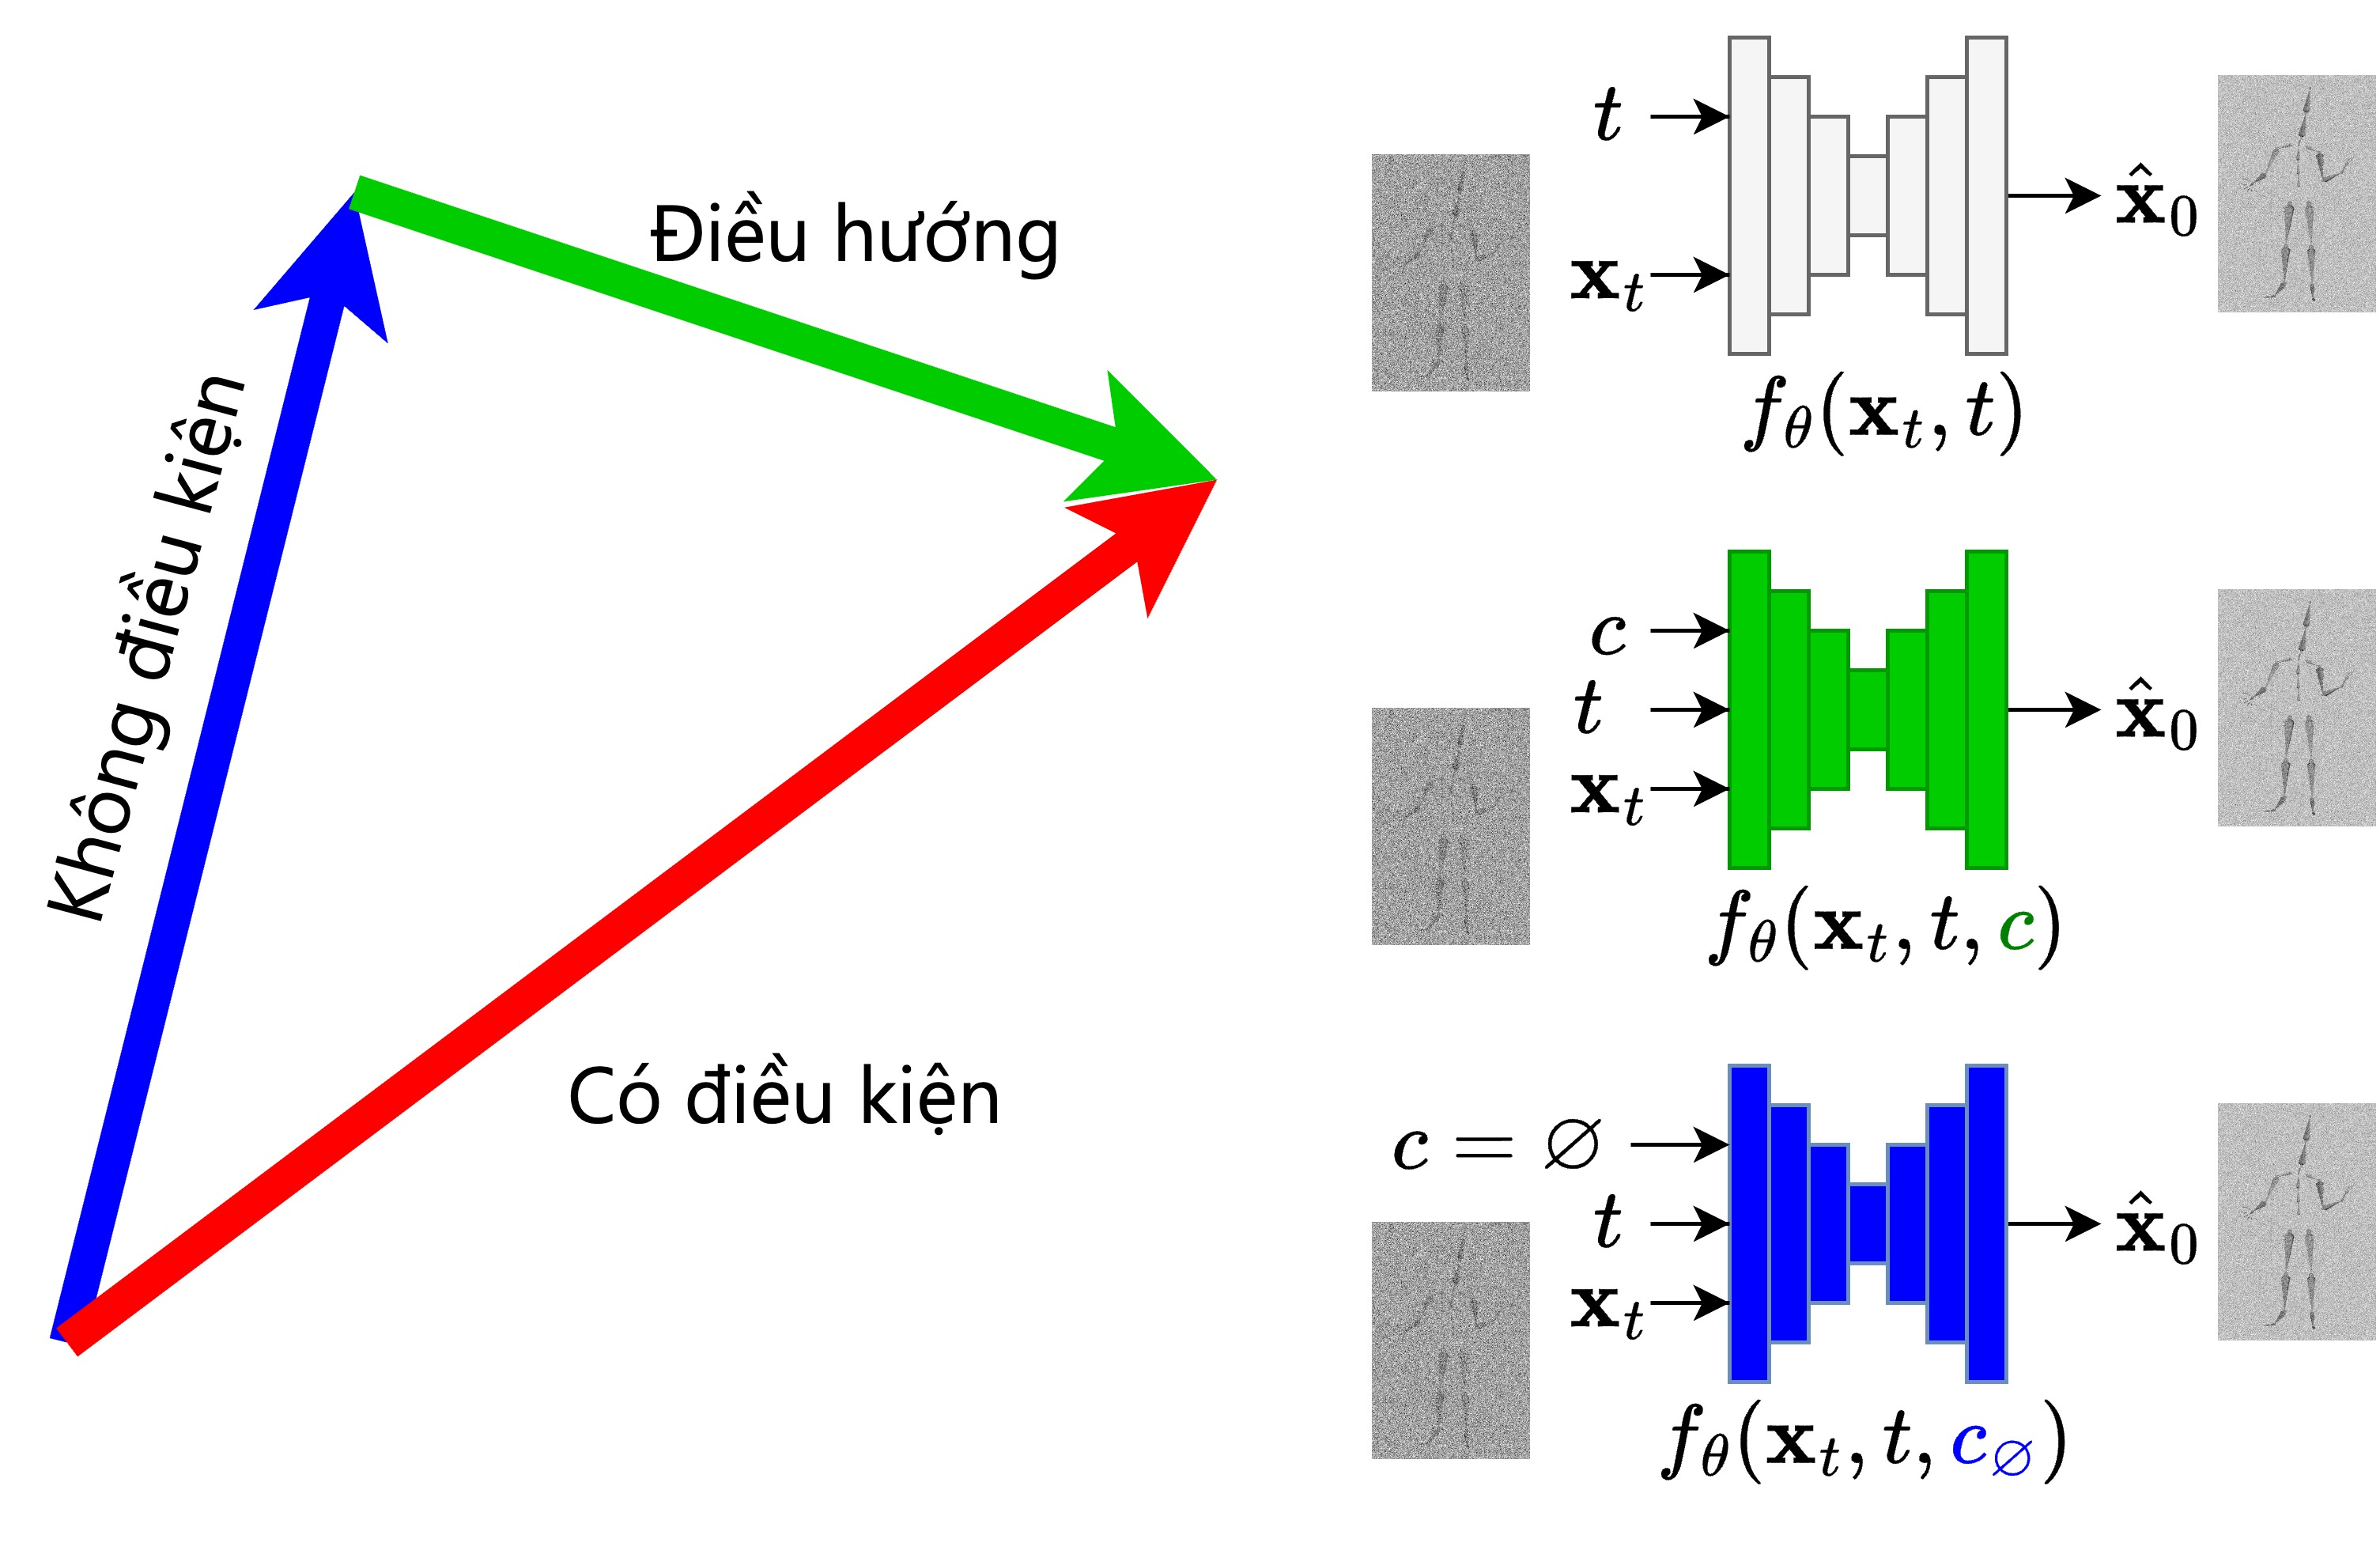
\includegraphics[width=0.9\linewidth]{AdversarialGradient}
	\caption{Diffusion có điều kiện bằng vector điều hướng}
	\label{fig:AdversarialGradient}
\end{figure}

Như hình \autoref{fig:GaussianDrift}, để quá trình suy luận có thể sinh ra các kết quả $\bx_0$ khác nhau và có thể điều khiển được dựa trên điều kiện $c$. Ở mỗi bước $t$, cần thêm một lượng điều hướng với một điều kiện cụ thể. Nhóm tác giả đề xuất  Classifier-Free Diffusion Guidance \cite{ho2022classifier} với việc kết quả $\bx_0$ được cập nhật bằng cách cộng kết quả có điều kiện và không có điều kiện.
\begin{equation}
{\color{red}{\hat{\mathbf{x}}}}_{0 \gamma, \color{blue}{c}, \color{green}{c_{\varnothing}}}=\gamma \cdot f_{\theta} \left(\mathbf{x}_{t}, t, {\color{blue}{c}} \right)+(1-\gamma) \cdot f_{\theta} \left(\mathbf{x}_{t}, t, {\color{green}{c_{\varnothing}}} \right)
\end{equation}

Trong đó, $c$ là điều kiện, $c_{\varnothing}$ là điều kiện rỗng,  kết quả sinh điều kiện được điều khiển bằng tham số $\gamma$, nếu $\gamma$ càng lớn thì kết quả sinh ra càng sát với điều kiện $c$, ngược lại thì kết quả sẽ nghiêng về kết quả sinh không có điều kiện.


Như \autoref{fig:AdversarialGradient}, hàm $f_{ \theta}$ trên cùng là không có điều kiện, $f_{ \theta}$ giữa là diffusion có điều kiện, $f_{ \theta}$ (dưới cùng) là diffusion với điều kiện rỗng.
\pagebreak

\section{Mô hình của đề xuất OHGesture}
\label{sec:ohgesture}

\begin{figure}[H]
	\centering
		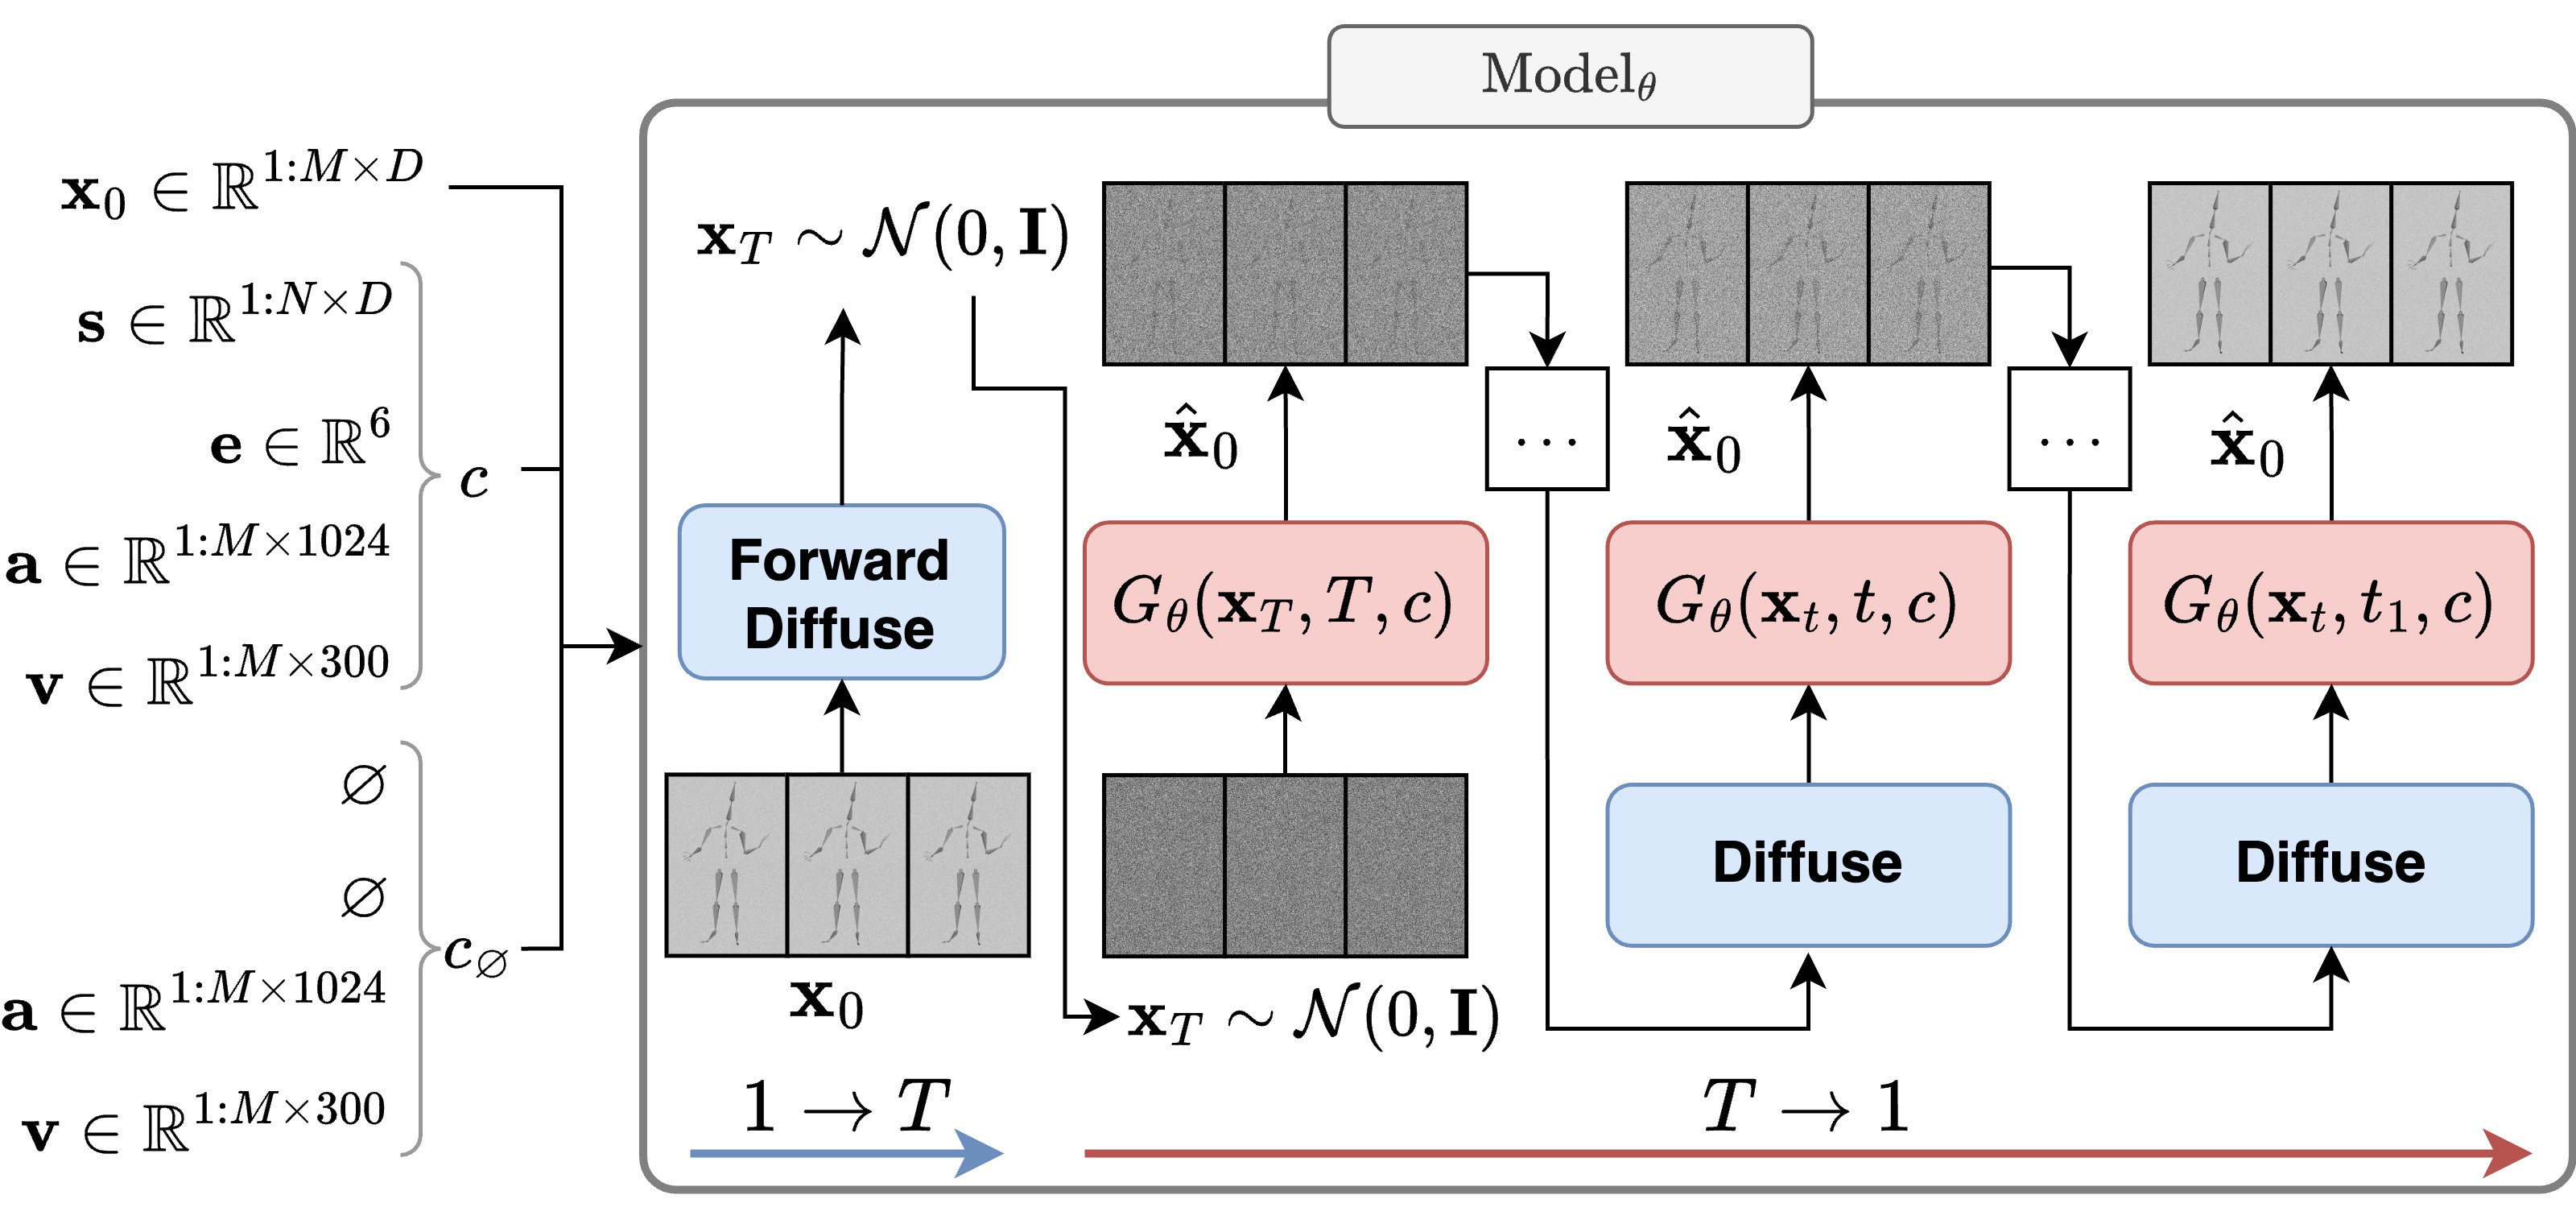
\includegraphics[width=\linewidth]{AllStage}
	\caption{Tổng quan về mô hình OHGesture}
	\label{fig:TrainingAndSampling}
\end{figure}

Mô hình đề xuất \textbf{OHGesture} (\textbf{O}pen \textbf{H}uman \textbf{Gesture} Generation) của luận văn được dựa trên mô hình \textbf{DiffuseStyleGesture} \cite{yang2023diffusestylegesture} áp dụng mô hình Diffusion \cite{ho2020denoising} có điều kiện \cite{ho2022classifier} (Classifier-Free Diffusion Guidance) để điều khiển các đặc trưng trong quá trình khử nhiễu.

Những điểm giống và khác của việc áp dụng mô hình diffusion cho bài toán sinh cử chỉ (gesture generation) so với mô hình Diffusion trong bài toán sinh ảnh:

\vspace{10pt}

\textbf{Điểm giống}
\begin{itemize}
	\item Sử dụng mô hình Diffusion (\autoref{sec:summary_diffusion}) trên cử chỉ $\bx^{1:M \times D}$,  với $M$ khung hình theo thời gian, $D=1141$ là các điểm tọa độ chuyển động của mỗi khung hình (tương tự width và height trong ảnh).
	\item Sử dụng Diffusion có điều kiện (\autoref{subsec:DiffusionCondition}) với $\bx_0$ objective (\autoref{subsec:X0Objective}).
	\item Ở công đoạn \textit{4. Mã hóa đặc trưng} và công đoạn \textit{6. Giải mã đặc trưng} \autoref{fig:CommonStage}, mô hình sử dụng latent vector có số chiều là $256$.
\end{itemize}

\textbf{Điểm khác}

\begin{itemize}
	\item Sinh cử chỉ có điều kiện:
	\begin{itemize}
		\item Điều kiện cảm xúc: $c = \big[ \mathbf{s}, \mathbf{e}, \mathbf{a}, \mathbf{v} \big]$ và $c_{\varnothing} = \big[ \varnothing, \varnothing, \mathbf{a}, \mathbf{v}\big]$.
		\item Nội suy trạng thái giữa hai cảm xúc $\mathbf{e}_1, \mathbf{e}_2$, sử dụng điều kiện: $c = \big[ \mathbf{s}, \mathbf{e}_1, \mathbf{a}, \mathbf{v} \big]$ và $c_{\varnothing} = \big[ \mathbf{s}, \mathbf{e}_2, \mathbf{a}, \mathbf{v} \big]$.
	\end{itemize}
	\item Ở công đoạn \textit{5. Kết hợp đặc trưng} \autoref{fig:CommonStage}, mô hình sử dụng Self-Attention: Mối liên hệ giữa các cảm xúc, cử chỉ khởi tạo và từng khung hình (tương tự DALL-E 2 tính mối liên hệ giữa văn bản và ảnh).
	\item Ở công đoạn \textit{5. Kết hợp đặc trưng} \autoref{fig:CommonStage}, mô hình concat giọng nói và văn bản (Tương tự như ControlNet sử dụng Pixel-wise Condition)
	%			\item Học mối liên hệ giữa điều kiện và các khung hình bằng Local-Cross Attention
\end{itemize}

Trong đó $\bx_0$ là chuỗi $M$ khung hình cử chỉ $\mathbf{x} \in \mathbb{R}^{1:M \times D}$ ($D = 1141$), với điều kiện $c = [\mathbf{s}, \mathbf{e}, \mathbf{a}, \mathbf{v}]$ bao gồm cử chỉ khởi tạo (seed gesture) $\mathbf{s}$,  cảm xúc (emotion) $\mathbf{e}$, chuỗi giọng nói (audio) $\mathbf{a}$ tương ứng cử chỉ, và văn bản  $\mathbf{v}$.

Mục tiêu của mô hình là học được tham số $\theta$ của hàm $G_{\theta}$ (\textbf{g}enerative) với đầu vào là ma trận cử chỉ $\bx^{1:M \times D}_t$, bước thời gian $t$ và điều kiện $c$.
Tổng quan của mô hình đề xuất \textbf{OHGesture} được minh họa ở hình \autoref{fig:TrainingAndSampling}. Tương tự mô hình diffusion cơ bản bao gồm hai quá trình: quá trình tạo nhiễu (diffusion) $q$ và quá trình khử nhiễu (denoising process) $p_{\theta}$ với trọng số $\theta$. Công đoạn \textit{1. Tiền xử lý} sẽ được trình bày ở \autoref{sec:Preprocessing}.

\subsection{Công đoạn xử lý đặc trưng}
Trong công đoạn \textit{2. Xử lý đặc trưng} (\autoref{fig:CommonStage}), mục tiêu là chuyển dữ liệu  thành các ma trận hoặc vector trước khi đưa vào mô hình.

\begin{itemize}
	\item \textbf{Văn bản} (Text):
		Như đã trình bày trong \autoref{subsec:TypicalMethod}, \textit{MDM} \cite{tevet2022human}, \textit{DiffuseStyleGesture+} \cite{yang2022DiffuseStyleGestureplus} trong công đoạn này sử dụng các đoạn văn bản mô tả cử chỉ như là Prompt của Midjourney làm đầu vào cho mô hình, tuy nhiên văn bản mô tả được dùng để phân cụm từng cử chỉ. Trong khi mục tiêu của luận văn là sử dụng văn bản như là một đặc trưng ngữ nghĩa, để căn chỉnh từng đoạn văn bản tương ứng với  từng đoạn cử chỉ phục vụ cho việc xây dựng người kỹ thuật số.
		
		Vì vậy, trong công đoạn này đóng góp của luận văn là sử dụng dữ liệu tiếng nói có sẵn, sau khi tiền xử lý ở \autoref{sec:Preprocessing} để thu được văn bản,  luận văn sử dụng mô hình FastText  \cite{bojanowski2017enriching} để nhúng (embedding) văn bản thành các vector căn chỉnh tương ứng với số khung hình tương ứng với cử chỉ. Với các vùng không có văn bản sẽ được cho là ma trận $\mathbf{0}$, các vùng có từ vựng tương ứng sẽ được gán là giá trị nhúng  theo từng khung hình của cử chỉ để được ma trận văn bản $\mathbf{v}^{1:M \times 300}$.
		
		\item \textbf{Giọng nói} (Speech): Tất cả dữ liệu giọng nói ở dạng wav sẽ được giảm số sample rate (downsampled) xuống $16 \mathrm{kHz}$, và giọng nói sẽ được lấy tương ứng với cử chỉ là 4s để được vector $\mathbf{a} \in \mathbb{R}^{64000}$. Tương tự DiffuseStyleGesture, luận văn sử dụng mô hình pre-train WavLM Large \cite{Chen_2022} nhúng waveform thô vào để được vector thể hiện đặc trưng âm thanh. Sau đó sử dụng nội suy tuyến tính (interpolation) để căn chỉnh đặc trưng của vector tiềm ẩn trong WavLM theo chiều thời gian thành $20 \text{fps}$ để được ma trận giọng nói $\mathbf{a} \in \mathbb{R}^{1:M \times 1024}$
		
		\item \textbf{Cảm xúc} (Emotion): Cảm xúc là nhãn được chọn 1 trong 6 cảm xúc bao gồm: $\texttt{Happy}$, $\texttt{Sad}$, $\texttt{Neutral}$, $\texttt{Old}$, $\texttt{Relaxed}$ và $\texttt{Angry}$. 
		
		Sau đó nhãn cảm xúc được đi qua lớp one-hot encoding để được vector  $\mathbf{e} \in \mathbb{R}^{6}$.
		
%		bao gồm 6 cảm xúc khác nhau được biểu diễn thành một vector theo phương pháp one-hot encoding, 
		
%		sau đó luận văn đưa qua một vector tuyến tính để được vector đặc trưng $\mathbf{E} \in \mathbb{R}^{64}$. Mục tiêu là để có thể concat được với vector khởi tạo $\mathbf{S} \in \mathbb{R}^{192} $ để tạo thành vector tiềm ẩn $256$ chiều. $\mathbf{E} \in \mathbb{R}^{64}$
		
		\item \textbf{Cử chỉ khởi tạo}: Cử chỉ khởi tạo (seed gesture) $\mathbf{s} \in \mathbb{R}^{1:N \times D}$ có được từ cử chỉ ground truth $
		\mathbf{g} \in \mathbb{R}^{(N+M) \times D}$, với mỗi khung hình là dữ liệu bao gồm $75$ khớp xương, được xử lý theo công thức \autoref{eq:gesturevector} để được vector $1141$ chiều, trình bày ở công thức \autoref{eq:gesturevector}. Mô hình của luận văn cắt $N = 8$ khung hình đầu để làm cử chỉ khởi tạo $\mathbf{s} \in \mathbb{R}^{1:N \times D} $
		
		\item \textbf{Cử chỉ thật}: Tương tự cử chỉ khởi tạo, từ $
		\mathbf{g} \in \mathbb{R}^{(N+M) \times D}$, luận văn sử dụng $M = 80$ (4 giây với $20fps$) khung hình là dữ liệu cử chỉ thật $\mathbf{x}_{0} \in \mathbb{R}^{1:M \times D}$. 
\end{itemize}

\subsection{Công đoạn trích xuất đặc trưng}
\label{subsec:feature_extraction}

Trong công đoạn \textit{3. Trích xuất đặc trưng} (\autoref{fig:CommonStage}), mục tiêu là chuyển ma trận thành các vector tiềm ẩn (latent vector) biểu diễn thông tin của dữ liệu bằng cách cho các đặc trưng cần học đi qua các lớp biến đổi tuyến tính (linear) hoặc MLP (Multilayer Perceptron).

\begin{figure}[H]
	\centering
	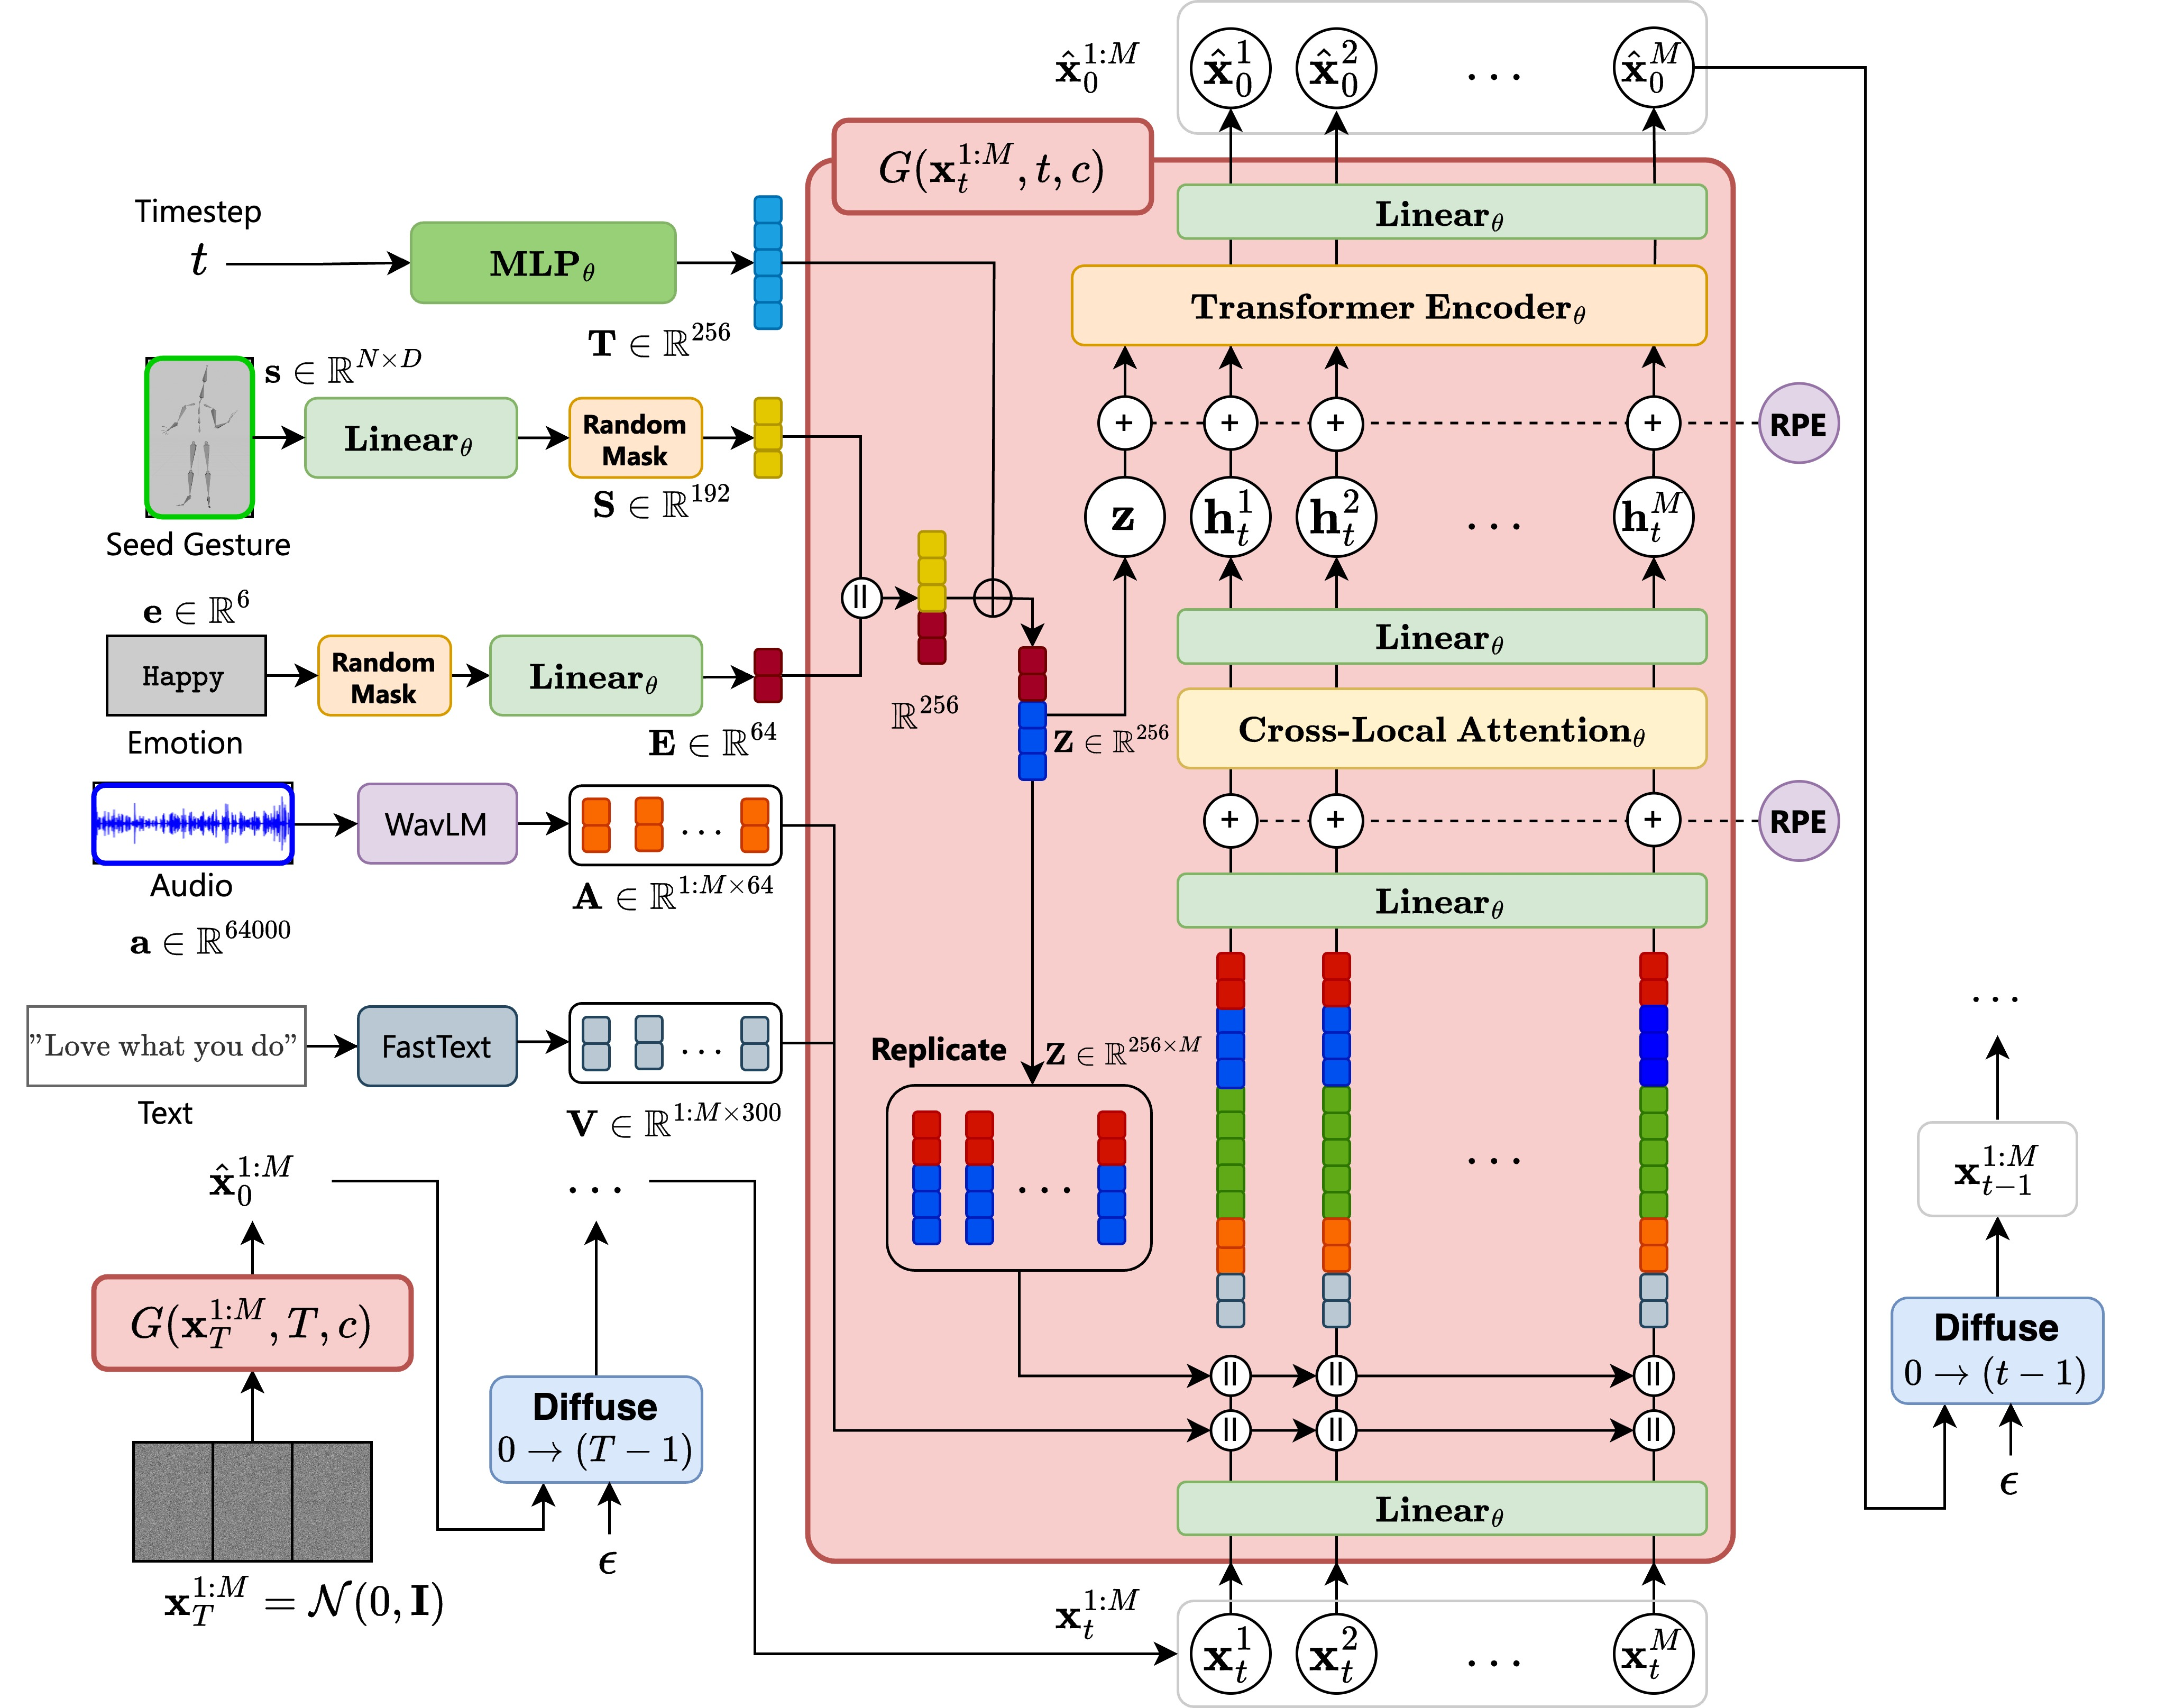
\includegraphics[width=\textwidth]{OHGesture}
	\caption{Mô hình trong OHGesture}
	\label{fig:OHGesture}
\end{figure}
\vspace{-10pt}

\begin{itemize}
	\item \textbf{Bước thời gian $\mathbf{T} \in \mathbb{R}^{256}$ }: Bước thời gian ở mỗi quá trình $t \in [0, T]$, mục tiêu của mô hình là để với bước thời gian $t$ bất kỳ, mô hình có thể tổng quát hóa quá trình khử nhiễu, và có thể học được việc với từng bước $t$ thì giá trị sẽ thay đổi thế nào đối với kết quả dự đoán $\bx_0$. Giá trị timestep $t$ được khởi tạo bằng việc mã hóa nhúng vị trí (Position Embedding) bằng hàm sinusoidal $\text{PE}(t) = \left[ \sin{\left(\frac{t}{10000^{2i / d}}\right)}, \cos{\left(\frac{t}{10000^{2i / d}}\right)} \right]$, sau đó được đưa vào một MLP (Multilayer perceptron) để biến đổi thành vector $\mathbf{T}  \in \mathbb{R}^{256}$.
	
	  \item \textbf{Giọng nói $\mathbf{A} \in \mathbb{R}^{1:M \times 64}$}: Từ giọng nói $\mathbf{a} \in \mathbb{R}^{1:M \times 1024}$ sẽ đi qua một lớp tuyến tính (linear layer) để giảm kích thước của đặc trưng xuống còn vector đặc trưng $64$ chiều để tạo thành ma trận cuối cùng $\mathbf{A} \in \mathbb{R}^{1:M \times 64}$.
	  
	  \item \textbf{Văn bản $\mathbf{V} \in \mathbb{R}^{1:M \times 64}$}: Văn bản $\mathbf{v}^{1:M \times 300}$ sẽ được đi qua lớp tuyến tính (linear layer) để căn chỉnh tương ứng với vector âm thanh.
	
	\item \textbf{Cử chỉ khởi tạo $\mathbf{S} \in \mathbb{R}^{192}$}: Từ $\mathbf{s} \in \mathbb{R}^{1:N \times D}$ sẽ được đi qua một lớp tuyến tính (linear layer) để được vector $\mathbf{S} \in \mathbb{R}^{192}$, vector $\mathbf{S}$ sau đó được đi qua một lớp mặt nạ ngẫu nhiên (random mask) trong quá trình huấn luyện để bỏ trong trường hợp nếu một trong $N$ khung hình bị thiếu thì sẽ ảnh hưởng như thế nào đến cử chỉ dự đoán.

  \item \textbf{Cảm xúc $\mathbf{E} \in \mathbb{R}^{64}$}: Từ vector cảm xúc $\mathbf{e} \in \mathbb{R}^{6}$ sẽ được đưa qua lớp tuyến tính (linear layer) để được vector đặc trưng $\mathbf{E} \in \mathbb{R}^{64}$. Mục tiêu là để có thể concat được với vector khởi tạo $\mathbf{S} \in \mathbb{R}^{192} $ để tạo thành vector tiềm ẩn $256$ chiều.
  
	\item \textbf{Cử chỉ nhiễu $\mathbf{x}_{T} \in \mathbb{R}^{1:M \times D}$} (Noisy gesture): khi huấn luyện, $\mathbf{x}_{t}$ là cử chỉ nhiễu có cùng kích thước như cử chỉ gốc $\mathbf{x}_{0}$ sẽ được sinh ngẫu nhiên từ phân phối chuẩn $\mathcal{N}(0, \mathbf{I})$. Khi sinh ngẫu nhiên, cử chỉ nhiễu ban đầu $\mathbf{x}_{T}$ được lấy mẫu từ phân phối Gaussian và các $\mathbf{x}_{t}, t<T$ khác là kết quả của bước làm nhiễu trước đó như \autoref{fig:TrainingAndSampling}.
%	Sau đó, kích thước được điều chỉnh thành 256  bằng lớp biến đổi tuyến tính (linear layer).
\end{itemize}


\subsection{Công đoạn mã hóa đặc trưng}

Trong công đoạn \textit{4. Mã hóa đặc trưng} (\autoref{fig:CommonStage}), mục tiêu là giảm số chiều của dữ liệu xuống kích thước thấp hơn, nhằm giảm việc bùng nổ khối lượng tính toán.

Với dữ liệu chính trong quá trình Diffusion chính là chuỗi cử chỉ $\bx_t \in \mathbb{R}^{1:M \times D}$. Như minh họa ở \autoref{fig:OHGesture}, chuỗi cử chỉ với kích thước $M \times D$ sẽ đi qua lớp $\operatorname{Linear}_{\theta}$ để được ma trận $\mathbf{X} \in \mathbb{R}^{1:M \times 256}$. Quá trình giảm chiều dữ liệu của $\bx$ sẽ được thực hiện trước khi chuỗi cử chỉ $\bx$ đi qua các lớp Cross-Local Attention và Transformer Encoder để tính sự tương quan giữa nhiều loại dữ liệu khác nhau.


\subsection{Công đoạn kết hợp đặc trưng}

Trong công đoạn \textit{5. Kết hợp đặc trưng} (\autoref{fig:CommonStage}), mục tiêu là sử dụng các phép concat, cộng hoặc các lớp attention để tính sự tương quan giữa các đặc trưng.

Đầu tiên cử chỉ khởi tạo $\mathbf{S} \in \mathbb{R}^{192}$ và vector cảm xúc $\mathbf{E} \in \mathbb{R}^{64}$ được ghép lại với nhau để tạo thành một vectơ có kích thước $256$, bởi vì kích thước $256$ là kích thước vector tiềm ẩn được chọn để tính tương quan giữa các đặc trưng. Sau đó được cộng thêm vector timestep $\mathbf{T}$ để tạo thành vector $\mathbf{z} \in \mathbb{R}^{256}$.

\begin{equation}
	\label{eq:ConditionConcat}
	\mathbf{z}_{tk} = \operatorname{concat }(\mathbf{E}\ || \  \mathbf{S}) + \mathbf{T}
\end{equation}

\subsubsection{Kết hợp đặc trưng theo khung hình}

Sau đó, $\mathbf{z}$  replicate $M$ lần để căn chỉnh kích thước tương đương với kích thước khung hình để được $\mathbf{Z} \in \mathbb{R}^{1:M \times 256}$

Ta sẽ cộng ma trận giọng nói và văn bản với nhau để được ma trận kết hợp thông tin của văn bản và giọng nói. Sau đó tiếp tục kết hợp concat với ma trận cử chỉ $\mathbf{X}$. Cuối cùng kết hợp với ma trận $\mathbf{Z}$ để được ma trận $\mathbf{H}$.

\begin{equation}
	\label{eq:FrameConcat}
	\mathbf{M} = \operatorname{concat}( \mathbf{Z}\  || \   \operatorname{concat}(\mathbf{X}\ || \  (\mathbf{V} + \mathbf{A}) ) )
\end{equation}

Sau khi có ma trận $\mathbf{M} \in \mathbb{R}^{1:M \times P}$ theo \autoref{eq:FrameConcat} thể hiện đặc trưng theo khung hình từ khung hình $1$ đến khung hình $M$, với mỗi khung hình có kích thước $P$ là tổng của các đặc trưng đã concat. Với $\mathbf{X} \in \mathbb{R}^{1:M \times 256}$, $\mathbf{Z} \in \mathbb{R}^{1:M \times 256}$ và $\mathbf{A}, \mathbf{V} \in \mathbb{R}^{1:M \times 64}$, thì $P$ sẽ có kích thước $256 * 2 + 64$. Sau đó, ma trận $\mathbf{m}$ sẽ được đi qua quá trình biến đổi tuyến tính: $\mathbf{m}^{1:M \times 256} = \operatorname{Linear}_{\theta}(M)$ để được ma trận $\mathbf{m} \in \mathbb{R}^{1:M \times 256}$.

\subsubsection{Cơ chế attention trong quá trình kết hợp các đặc trưng}

Trong mô hình của luận văn, mục tiêu của việc áp dụng cơ chế attention là tìm được sự tương quan của từng khung hình với nhau.

Lớp attention có công thức như sau:

\begin{equation} \label{eq:attention}
	\operatorname{Attention}(\mathbf{Q}, \mathbf{K}, \mathbf{V}, \mathbf{M})=\operatorname{softmax}\left(\frac{\mathbf{Q} \mathbf{K}^{T}+\mathbf{M}}{\sqrt{C}}\right) \mathbf{V}
\end{equation}

Công thức Attention trên có $\mathbf{Q}$, $\mathbf{K}$ ,$\mathbf{V}$ là các ma trận sau khi đi qua các ma trận biến đối tuyến tính $\mathbf{Q} = \mathbf{X} \mathbf{W}_Q$, $\mathbf{K} = \mathbf{X} \mathbf{W}_K$, $\mathbf{V} = \mathbf{X} \mathbf{W}_V$. Với đầu vào là ma trận biểu thị chuỗi $M$ khung hình, với mỗi khung hình là một vector được concat từ các vector đặc trưng bao gồm cả cử chỉ khởi tạo, văn bản, giọng nói, cảm xúc và cử chỉ $\bx_t$ mà luận văn muốn thực hiện khử nhiễu. Quá trình Local-Cross Attention được điều khiển chỉ để tính các đặc trưng cục bộ của chuyển động của các cử chỉ và đặc trưng trong các khung hình lân cận.

\begin{figure}[H]
	\centering
	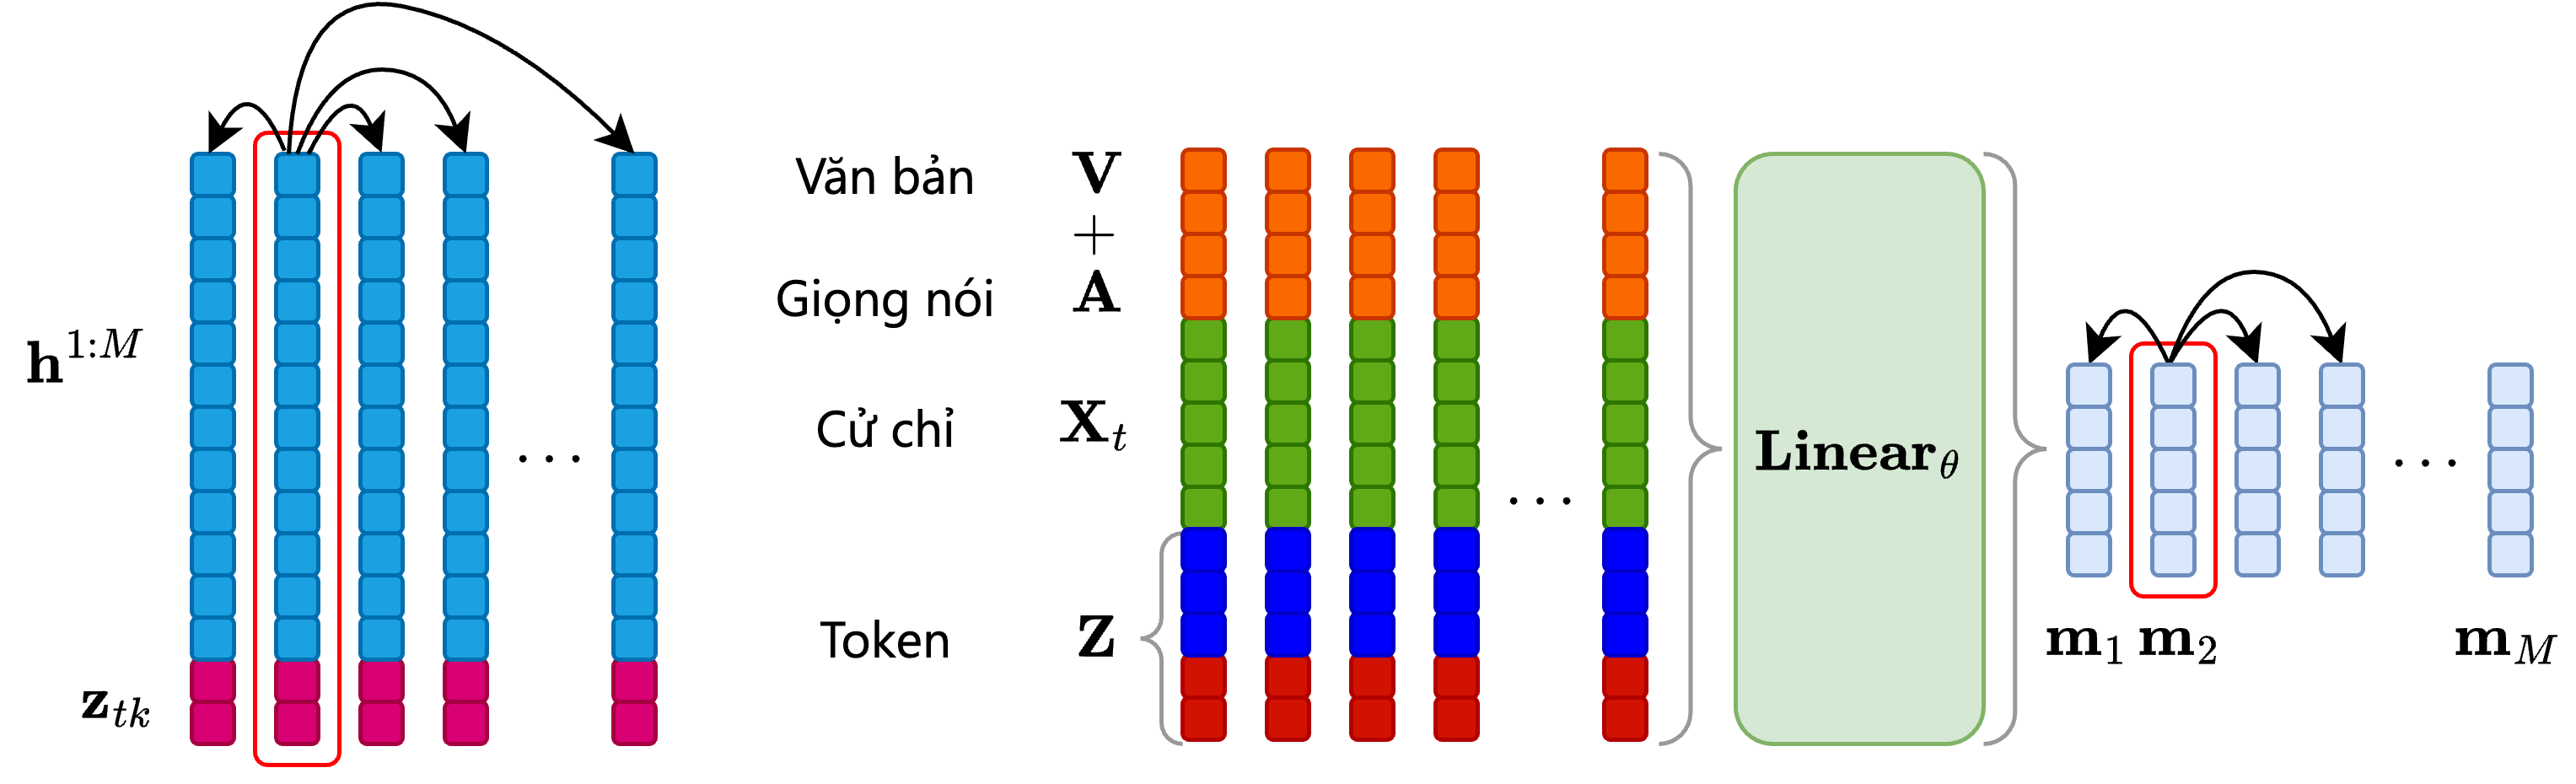
\includegraphics[width=\textwidth]{CrossLocalAttention}
	\caption{Cơ chế Attention trong Transformer Encoder và Cross-Local Attention}
	\label{fig:CrossLocalAttention}
\end{figure}

Hàm Attention hoạt động như một bộ từ điển, với các thông tin cuối cùng tra được là ma trận $\mathbf{V}$ (value), còn $\mathbf{Q}$ (query) là từ khóa muốn tìm kiếm, $\mathbf{K}$ (key) là danh mục các từ khóa trong bộ từ điển tra cứu. Quá trình Attention sẽ tính toán mức độ tương đồng giữa \( \mathbf{Q} \) và \( \mathbf{K} \) để xác định trọng số cho các giá trị trong \( \mathbf{V} \). 

Kết quả cuối cùng là tổ hợp các giá trị trong \( \mathbf{V} \), trong đó các giá trị tương ứng với các khóa giống truy vấn nhất sẽ có trọng số cao hơn. $\mathbf{M}$ là mặt nạ (mask) để thực hiện quá trình chú ý cục bộ. Cross-Local Attention sẽ được minh họa như \autoref{fig:CrossLocalAttention} bên phải. Còn lớp Transformer Encoder sẽ sử dụng Self-Attention lớp bên trái.

\subsubsection{Kết hợp đặc trưng cục bộ với Cross-Local Attention}

Ma trận $\mathbf{m} \in \mathbb{R}^{1:M \times 256}$ sẽ tiếp tục đi qua lớp Cross-Local Attention để tính tương quan giữa các đặc trưng cục bộ: 

\begin{equation}
	\mathbf{h}^{1:M}_{t}  = \operatorname{Linear}_{\theta}  ( \operatorname{Cross-Local\ Attention}( \mathbf{m}) )
	\label{eq:CrossLocalAttention}
\end{equation}

Cross-local Attention sẽ thực hiện với $\operatorname{Query} = \operatorname{Key} = \operatorname{Value} = \mathbf{m}$. 
Tương tự ý tưởng từ phương pháp Routing Transformer \cite{roy2021efficient}, Cross-local Attention cho thấy rằng sự quan trọng trong việc xây dựng biểu diễn các vector đặc trưng trung gian trước khi đi qua lớp Transformer Encoder như \autoref{fig:OHGesture}. 
Các vector đặc trưng sẽ được cộng thêm một vector mã hóa vị trí tương đối (Relative position encoding \cite{vaswani2017attention}) để thể hiện được đặc trưng thời gian trước khi đi qua lớp Cross-Local Attention.


Sau quá trình Cross-Local Attention, mô hình tiếp tục được đưa qua lớp tuyến tính theo \autoref{eq:CrossLocalAttention} để căn chỉnh tương ứng với $M$ khung hình, bao gồm $\mathbf{h}^{1:M}$.


\subsubsection{Kết hợp đặc trưng toàn cục với Transformer Encoder}

\begin{figure}[H]
	\centering
	\begin{subfigure}{0.42\textwidth}
		\centering
		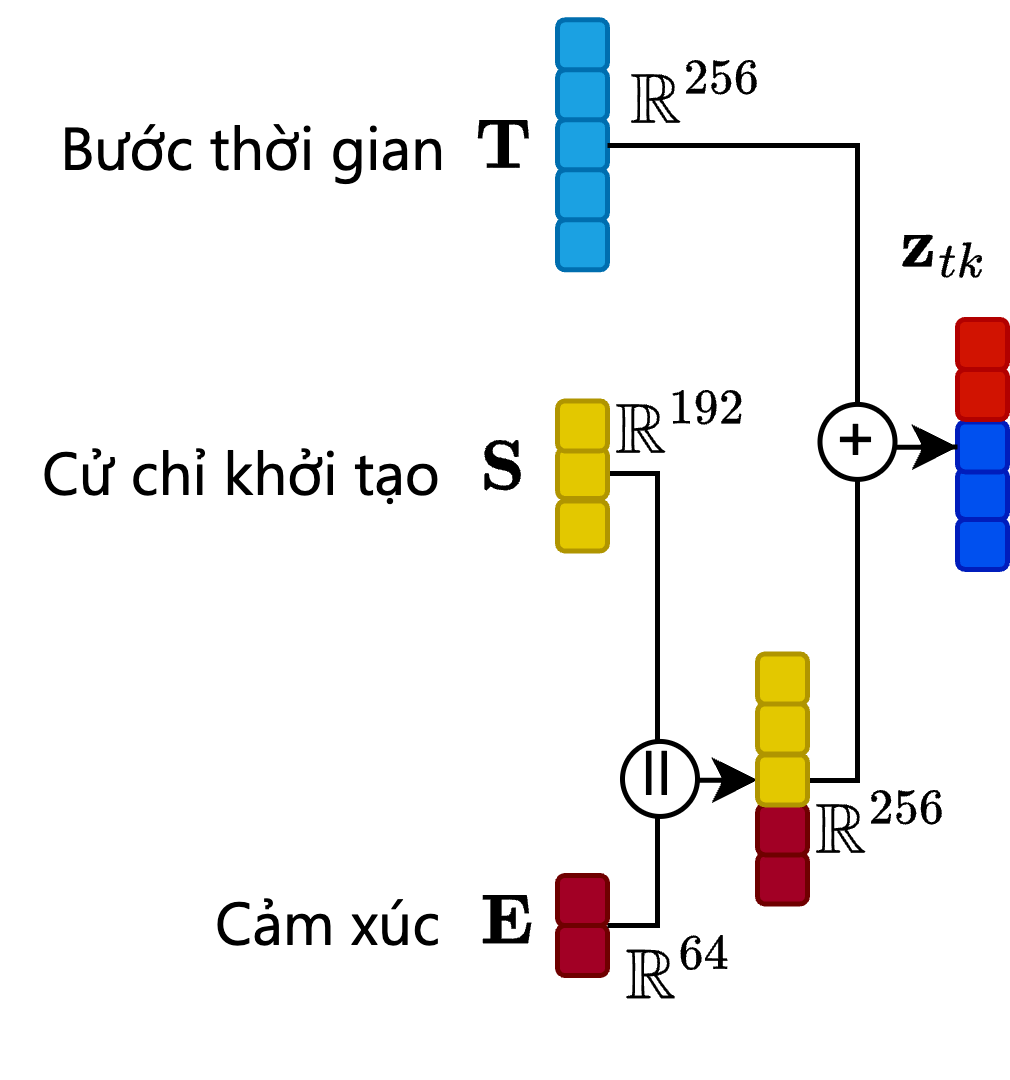
\includegraphics[width=\textwidth]{z}
		\caption{Cách concat đặc trưng để được $\mathbf{z}_{tk}$}
		\label{fig:FeatureFusion}
	\end{subfigure}
	\hfill
	\begin{subfigure}{0.55\textwidth}
		\centering
		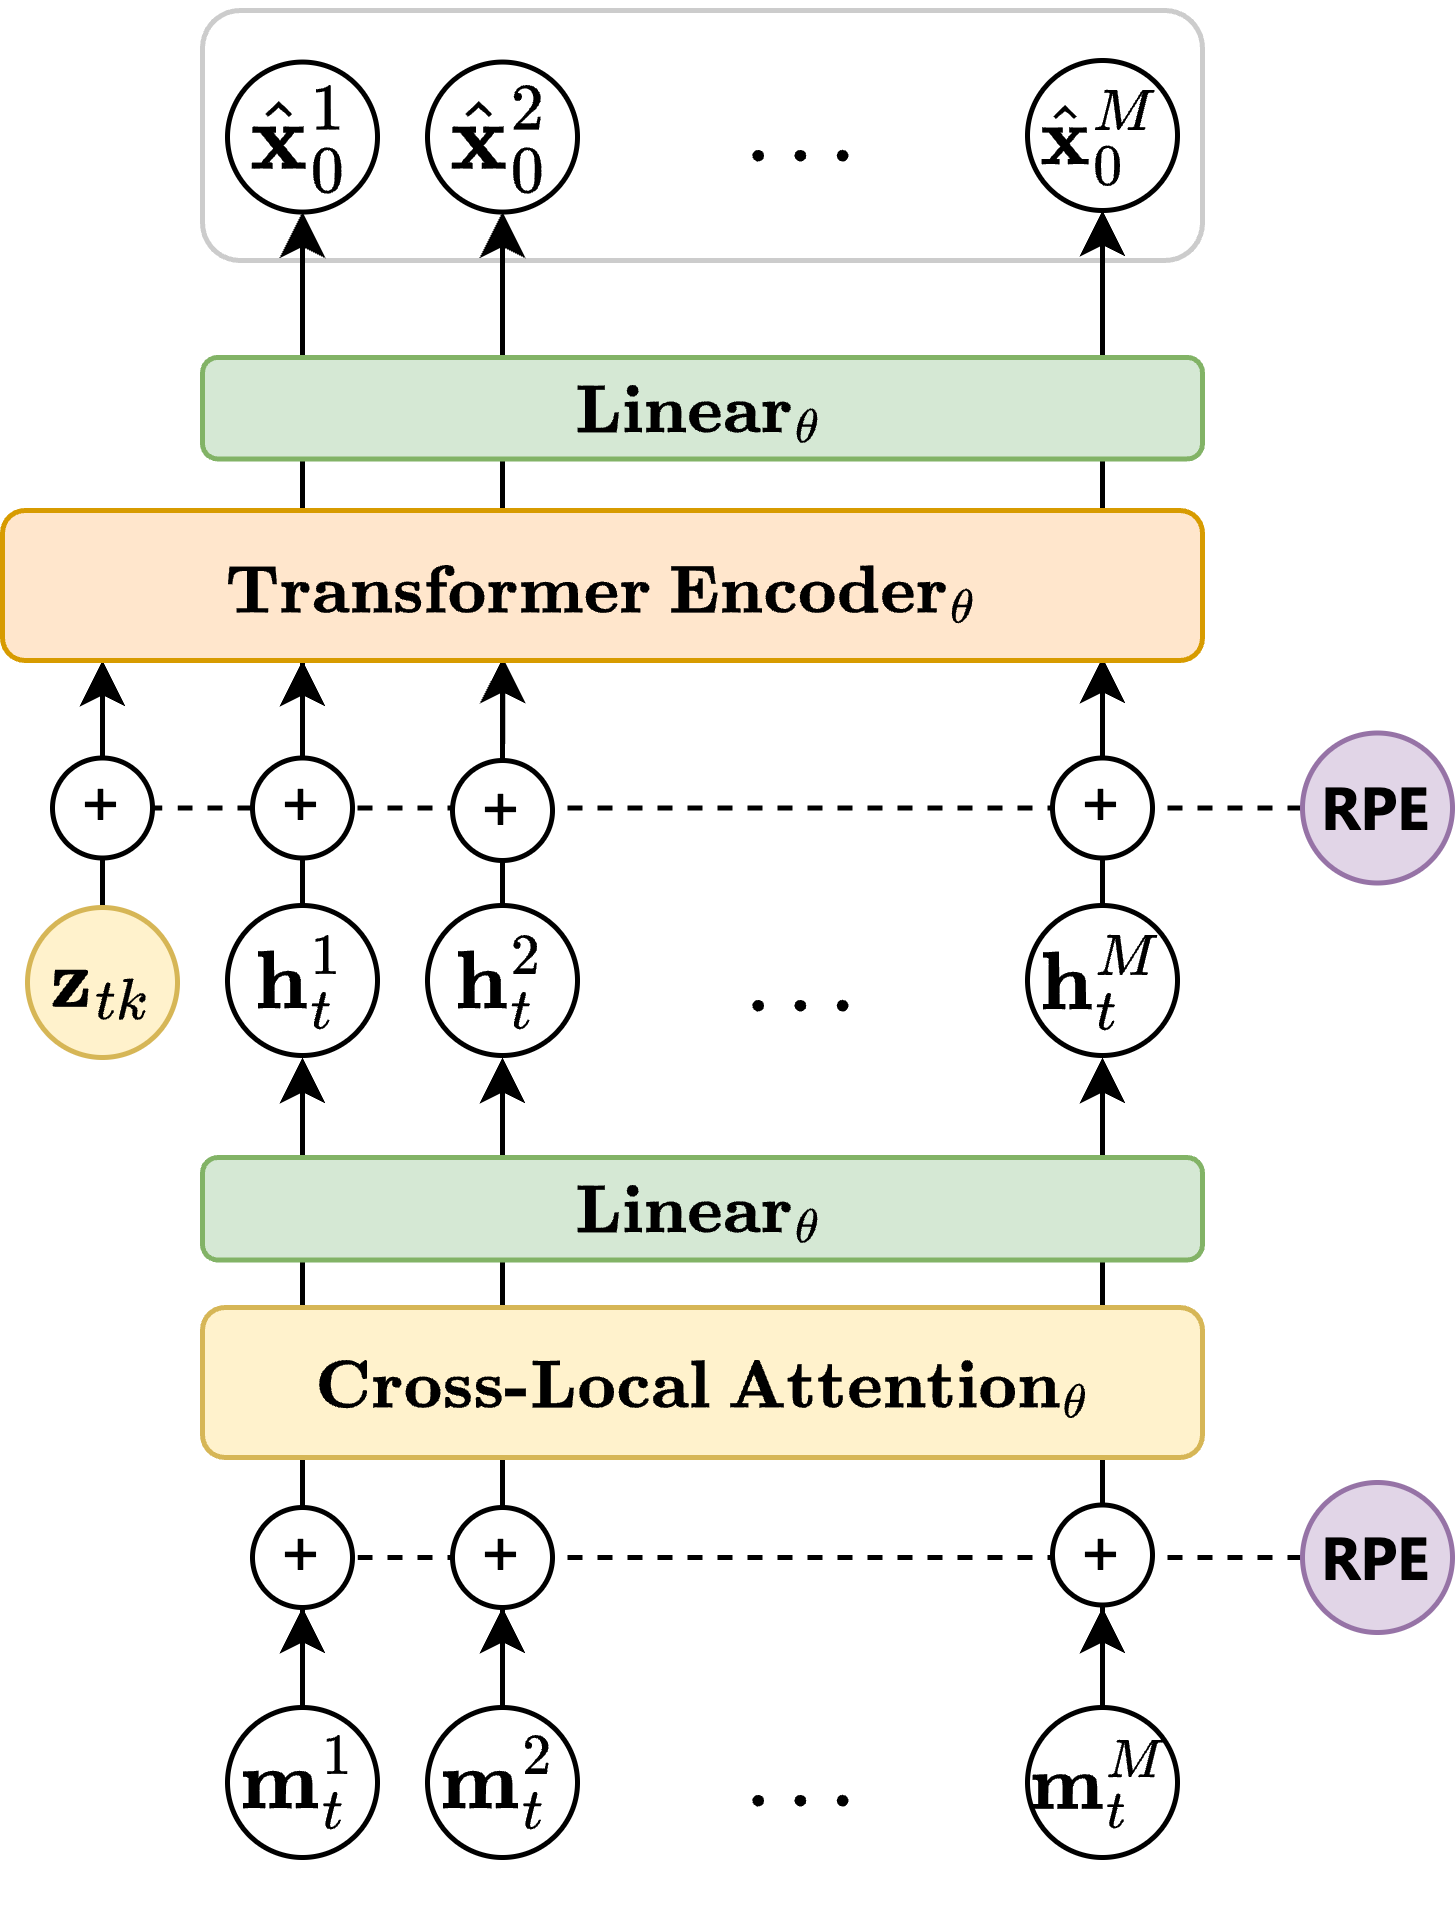
\includegraphics[width=\textwidth]{FeatureFusion}
		\caption{Quá trình kết hợp đặc trưng theo từng khung hình}
		\label{fig:ZToken}
	\end{subfigure}
\end{figure}


Kế thừa từ MDM \cite{tevet2022human}, vector $\mathbf{z}$ là token đầu tiên thể hiện thông tin cho toàn bộ chuỗi khung hình, tương tự như  $z_{\text{tk}}$ trong mô hình BERT \cite{devlin2019bertpretrainingdeepbidirectional}, với token $\texttt{CLS}$ đầu tiên thể hiện thông tin của toàn bộ đoạn văn bản.
Ở đây, luận văn sử dụng $z_{\text{tk}}$ là $\mathbf{z} \in \mathbb{R}^{256}$ (\autoref{eq:ConditionConcat}) token đầu tiên biểu thị đặc trưng biểu thị cho toàn bộ chuỗi $M$ khung hình.

\begin{equation}
	\mathbf{x}^{1:M}_{0}  = \operatorname{Transformer\ Encoder}( \operatorname{concat}( \mathbf{z}_{tk} \ ||\  \mathbf{h}^{1:M}_{t}  )))
	\label{eq:TransformerEncoder}
\end{equation}


Các vector $\mathbf{h}$ biểu thị cho chuỗi $M$ khung hình, tương tự như phương pháp Reformer \cite{kitaev2020reformer}, trước khi đi vào lớp Self-Attention trong Transformer Encoder, mô hình sẽ sử dụng lớp mã hóa vị trí tương đối (Relative Position Encoding - RPE) để thay thế mã hóa vị trí tuyệt đối, giúp mô hình hiệu quả hơn trong việc xử lý chuỗi dài.
Khi vào lớp Transformer Encoder \cite{vaswani2017attention} giúp tính toán được mối liên hệ giữa các chuỗi dữ liệu. 
Trong lớp Transformer Encoder mô hình sẽ áp dụng cơ chế tự chú ý tương tự như \autoref{eq:attention} trên nhưng không sử dụng mặt nạ. 


\subsection{Công đoạn giải mã đặc trưng}

Trong công đoạn \textit{6. Giải mã đặc trưng} (\autoref{fig:CommonStage}), sau khi tính được sự tương quan giữa các đặc trưng, mục tiêu là tăng kích thước dữ liệu trở về kích thước ban đầu.

Như minh họa ở \autoref{fig:OHGesture}, ma trận tiềm ẩn, sau khi đi qua lớp Transformer Encoder để tính sự tương quan giữa nhiều loại dữ liệu khác nhau. Kết quả sẽ đi qua lớp $\operatorname{Linear}_{\theta}$ để tăng kích thước ma trận tiềm ẩn thành kích thước ban  đầu $\hat{\mathbf{x}}_{0} \in \mathbb{R}^{1:M \times D}$.

Công đoạn cuối cùng, kết xuất sẽ được trình bày ở \autoref{sec:Render}.

\subsection{Điều khiển cảm xúc trong bài toán sinh cử chỉ}

Ở các bước trên mô hình đã có thể học được cách sinh cử chỉ.
Tuy nhiên, để mô hình học được các cảm xúc trong các tình huống khác nhau, luận văn tham số hóa và thay đổi lần lượt từng cảm xúc, sao cho kết quả dự đoán phản ánh đúng cảm xúc tương ứng.

Tương tự như các phương pháp sử dụng mô hình khử nhiễu có điều kiện \cite{ho2022classifier}, \cite{tevet2022human}, luận văn sử dụng điều kiện $c = [ \mathbf{s}, \mathbf{e}, \mathbf{a}, \mathbf{v} ]$,  bao gồm cử chỉ khởi tạo $\mathbf{s}$, cảm xúc $\mathbf{e}$, giọng nói tương ứng $\mathbf{a}$ và văn bản $\mathbf{v}$. Mô hình diffusion có điều kiện $c$ ở đây sẽ là tổng cả trường hợp ở từng bước $t$ trong mô hình khử nhiễu $\text{G}_\theta \left( \bx_{t}, t, c \right)$, với  $c_{\varnothing}=[\varnothing, \varnothing, \mathbf{a}, \mathbf{v}]$ không điều kiện và $c = [\mathbf{s}, \mathbf{e}, \mathbf{a}, \mathbf{v}]$ có điều kiện. Quá trình này có thể dễ dàng điều khiển bằng một lớp mặt nạ ngẫu nhiên (random mask) trên các vector đặc trưng của cử chỉ khởi tạo $\mathbf{s}$ và cảm xúc $\mathbf{e}$. Khi đó, mô hình chỉ việc thay đổi nhãn tương ứng với lớp mask đã lấy ngẫu nhiên để mô hình có thể tối ưu theo các điều kiện khác nhau. 


\begin{equation} \label{eq:denoise}
\hat{\bx}_{0 c, c_{\varnothing}, \gamma}=\gamma \cdot G \left(\bx_{t}, t, c\right)+(1-\gamma) \cdot G \left(\bx_{t}, t, c_{\varnothing}\right)
\end{equation}

Điểm đặc biệt là có thể dựa trên việc học có điều kiện và không có điều kiện của classifier-free guidance \cite{ho2022classifier}, có thể nội suy giữa hai cảm xúc $\mathbf{e}_1$ và cảm xúc $\mathbf{e}_2$ khác nhau bằng cách cho điều kiện $c = \left[\mathbf{s}, \mathbf{e}_{1}, \mathbf{a}, \mathbf{v} \right]$ và $c_\varnothing = \left[\mathbf{s}, \mathbf{e}_{2}, \mathbf{a}, \mathbf{v} \right]$. Khi đó ta có thể viết lại $\hat{x}_{0 \gamma, c_{1}, c_{2}}=\gamma  \cdot G \left(x_{t}, t, c_{1} \right)+(1-\gamma) \cdot G \left(x_{t}, t, c_{2}\right)$.


\subsection{Quá trình huấn luyện}


\begin{algorithm}[H]
	\caption{Huấn luyện trong OHGesture}
	\label{alg:trainingohgesture}
	\setlength{\baselineskip}{10pt}
	\begin{enumerate}
		\item Tính sẵn các giá trị và siêu tham số: $\gamma$, $\sqrt{\alpha_t}$, $\sqrt{1 - \alpha_t}$, $\sqrt{\bar{\alpha}_t}$ và nhiễu ngẫu nhiên $\boldsymbol{\epsilon}_t$ tại mỗi bước $t: 1 \rightarrow T$. Định nghĩa lịch nhiễu $\{\alpha_t \in (0, 1)\}_{t=1}^T$.
		
		\item Lấy nhãn ban đầu $\mathbf{x}_0$ từ phân phối dữ liệu đã chuẩn hóa.
		
		\item Tạo ngẫu nhiên các mặt nạ Bernoulli $c_{1} = \big[ \mathbf{s}, \mathbf{e_1}, \mathbf{a}, \mathbf{v} \big]$, $c_{2} = \big[ \mathbf{s}, \mathbf{e_2}, \mathbf{a}, \mathbf{v} \big]$, hoặc $c_{2} = \big[ \varnothing, \varnothing, \mathbf{a}, \mathbf{v} \big]$.
		
		\item Thêm nhiễu để có cử chỉ nhiễu $\mathbf{x}_t$:
		\[
		\mathbf{x}_t = \sqrt{\bar{\alpha}_t} \mathbf{x}_0 + \sqrt{1 - \bar{\alpha}_t} \boldsymbol{\epsilon}_t
		\]
		
		\item Với mỗi bước $t$, lấy \textbf{ngẫu nhiên} $t$ từ $[1, T]$.
		
		\item Với $\mathbf{x}_t$, $t$ và các điều kiện mặt nạ $c_1$, $c_2$, dự đoán chuỗi cử chỉ:
		\[
		\hat{\mathbf{x}}_{0 \gamma, c_{1}, c_{2}} = \gamma \cdot G_{\theta} \left(\mathbf{x}_{t}, t, c_{1}\right) + (1 - \gamma) \cdot G_{\theta} \left(\mathbf{x}_{t}, t, c_{2}\right)
		\]
		
		\item Tính loss và đạo hàm để cập nhật trọng số $\theta$:
		\[
		\mathcal{L}_t = \mathbb{E}_{t \sim [1, T], \mathbf{x}_0, \boldsymbol{\epsilon}_t} \left[ \operatorname{HuberLoss}(\mathbf{x}_0, \hat{\mathbf{x}}_0 ) \right]
		\]
		
		\item Lặp lại từ bước 6 cho đến khi hội tụ, thu được các tham số tối ưu $\theta'$.
	\end{enumerate}
\end{algorithm}


\autoref{alg:trainingohgesture} huấn luyện mô hình OHGesture bắt đầu bằng việc tính toán các giá trị và siêu tham số cần thiết như $\gamma$, $\sqrt{\alpha_t}$, $\sqrt{1 - \alpha_t}$, $\sqrt{\bar{\alpha}_t}$ và nhiễu ngẫu nhiên $\boldsymbol{\epsilon}_t$ cho từng bước thời gian $t$ từ 1 đến $T$. Sau đó, nhãn ban đầu $\mathbf{x}_0$, đại diện cho cử chỉ gốc, được lấy từ phân phối dữ liệu đã chuẩn hóa. Tiếp theo, các mặt nạ Bernoulli $c_1$ và $c_2$ được tạo ngẫu nhiên, mô phỏng các điều kiện khác nhau như cử chỉ, cảm xúc, giọng nói, hoặc văn bản, với một trong các mặt nạ có thể là không có thông tin cảm xúc. Sau khi có các mặt nạ, nhiễu được thêm vào để tạo thành cử chỉ nhiễu $\mathbf{x}_t$, được tính bằng công thức kết hợp chuỗi cử chỉ gốc và nhiễu ngẫu nhiên. Quá trình tiếp theo là chọn ngẫu nhiên một bước thời gian $t$ trong khoảng $[1, T]$ và sử dụng cử chỉ nhiễu $\mathbf{x}_t$ cùng các mặt nạ để dự đoán lại chuỗi cử chỉ gốc thông qua mô hình, trong đó dự đoán được tính bằng một sự kết hợp của các hàm tạo ra từ các điều kiện mặt nạ. Sau khi có dự đoán, loss được tính bằng cách sử dụng HuberLoss giữa chuỗi cử chỉ gốc và dự đoán, từ đó đạo hàm loss để cập nhật các tham số trọng số $\theta$. Quá trình huấn luyện này được lặp lại cho đến khi mô hình hội tụ và thu được các tham số tối ưu $\theta'$.


\subsection{Quá trình lấy mẫu}

\begin{figure}[H]
	\centering
	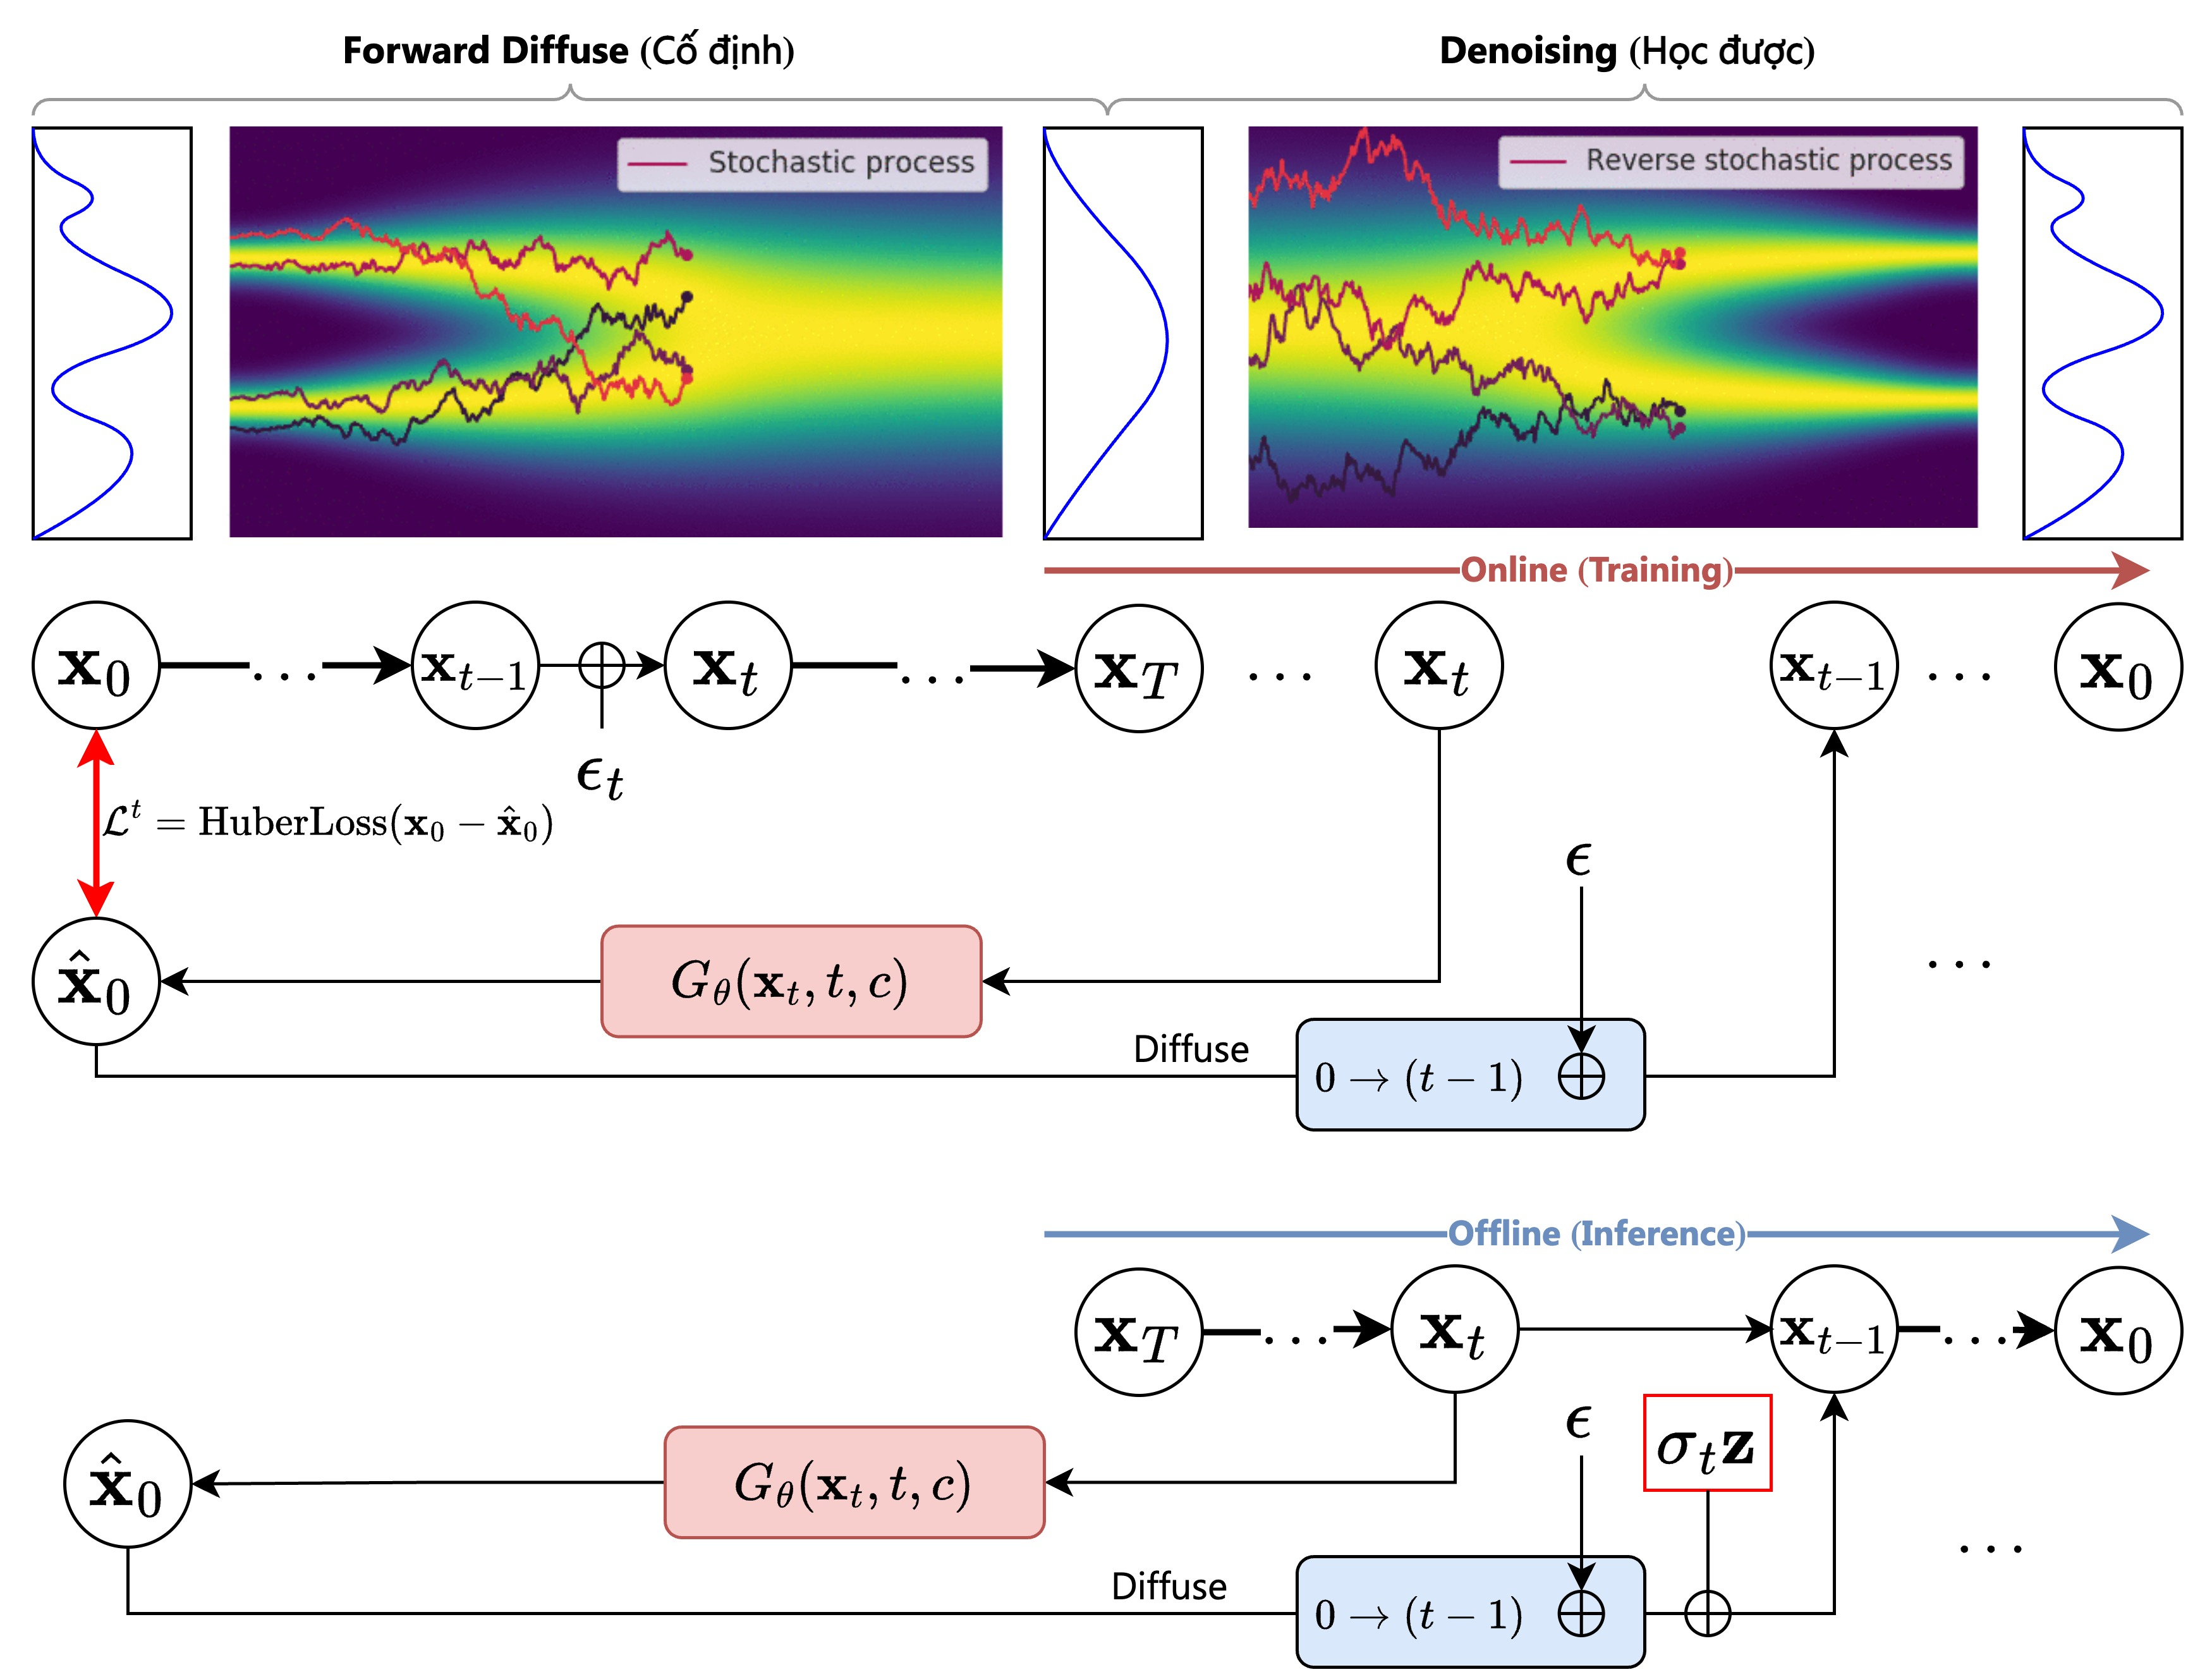
\includegraphics[width=\linewidth]{OnlineAndOffline}
	\caption{Quá trình học Offline (Training) và Online (Inference)}
	\label{fig:OnlineAndOffline}
\end{figure}

Để có thể sinh cử chỉ với chiều dài tùy ý, luận văn cắt chuỗi ban đầu thành các đoạn ngắn có chiều dài $M$. 
Trong quá trình huấn luyện, cử chỉ khởi tạo ban đầu có thể được tạo ra bằng cách lấy ngẫu nhiên một cử chỉ từ tập dữ liệu hoặc tính trung bình các đoạn đã cắt. Cụ thể ở đây, sẽ lấy góc quay trung bình trong các đoạn đã cắt được. Khi đó, chỉ cần lấy lần lượt các khung hình đã sinh ra và chọn $N = 8$ khung hình cuối cùng làm cử chỉ khởi tạo ở lượt tiếp theo. Đối với mỗi đoạn đã cắt ra, cử chỉ $\bx_{t}$ lần lượt sẽ được áp dụng hàm khử nhiễu $\hat{\bx}_{0} = G_{\theta'} \left( \bx_{t}, t, c\right)$, sau khi có $\hat{\bx}_{0}$ sẽ được thêm nhiễu (diffuse) cho đến khi được $\bx_{t-1}$, và $\bx_{t-1}$ sẽ tiếp tục được thực hiện khử nhiễu cho đến bước $t=1$ để được $\bx_{0}$.

\begin{algorithm}
	\caption{Lấy mẫu (sampling) trong OHGesture}
	\label{alg:sampling}
	\setlength{\baselineskip}{10pt}
	\begin{enumerate}
		\item Khởi tạo với nhiễu: $\mathbf{x}_T \sim \mathcal{N}(0, \mathbf{I})$.
		
		\item Các giá trị $\sqrt{\alpha_t}$, $\sqrt{1 - \alpha_t}$ và $\sqrt{\bar{\alpha}_t}$ lấy từ quá trình huấn luyện, tính sẵn giá trị $\sigma_t$ từ $\alpha_t$ ở mỗi bước $t: 1 \rightarrow T$.
		
		\item Chia mỗi đoạn giọng nói 4 giây thành: $\mathbf{a} \in \mathbb{R}^{64000}$. Cử chỉ khởi tạo $\mathbf{s}$ ban đầu là trung bình dữ liệu, sau đó được lấy từ đoạn cử chỉ đã suy luận. Chọn cảm xúc mong muốn, văn bản được phiên âm từ giọng nói $\mathbf{a}$, tạo cặp điều kiện $c = [\mathbf{s}, \mathbf{e}, \mathbf{a}, \mathbf{v}]$.
		
		\item Với mỗi $t$, lấy $t$ \textbf{tuần tự} từ $[T, \dots, 1]$.
		
		\item Tạo nhiễu ngẫu nhiên $\mathbf{z} \sim \mathcal{N}(0, \mathbf{I})$.
		
		\item Đưa $\mathbf{x}_t$ vào để suy luận $\hat{\mathbf{x}}_0^{(t)} = G_{\theta'}(\mathbf{x}_t, t, c)$.
		
		\item Thực hiện thêm nhiễu $\hat{\mathbf{x}}_0^{(t)}$ từ bước $0 \rightarrow t$ để nhận $\hat{\mathbf{x}}_{t-1}^{(t)}$.
		
		\item Cộng thêm nhiễu: $\hat{\mathbf{x}}_{t-1} = \hat{\mathbf{x}}_{t-1}^{(t)} + \sigma_t \mathbf{z}$.
		
		\item Quay lại bước 4. Khi $t = 1$, thu được $\hat{\mathbf{x}}_0$ từ quá trình khử nhiễu.
	\end{enumerate}

\end{algorithm}

\autoref{alg:sampling} lấy mẫu bắt đầu bằng việc khởi tạo cử chỉ nhiễu ban đầu $\mathbf{x}_T$ từ phân phối chuẩn $\mathcal{N}(0, \mathbf{I})$. Sau đó, các giá trị $\sqrt{\alpha_t}$, $\sqrt{1 - \alpha_t}$ và $\sqrt{\bar{\alpha}_t}$ được lấy từ quá trình huấn luyện, cùng với giá trị $\sigma_t$ được tính từ $\alpha_t$ tại mỗi bước thời gian $t$ từ 1 đến $T$. Mỗi đoạn giọng nói 4 giây được chia thành các chuỗi dữ liệu $\mathbf{a}$, và cử chỉ khởi tạo $\mathbf{s}$ được lấy từ trung bình dữ liệu hoặc từ đoạn cử chỉ đã suy luận. 
Cảm xúc mong muốn và văn bản được phiên âm từ giọng nói $\mathbf{a}$, tạo thành một cặp điều kiện $c = [\mathbf{s}, \mathbf{e}, \mathbf{a}, \mathbf{v}]$. Thuật toán sau đó thực hiện các bước tuần tự, bắt đầu từ bước cuối cùng $T$ và tiến ngược về 1. Ở mỗi bước, nhiễu ngẫu nhiên $\mathbf{z}$ được tạo ra và mô hình dự đoán $\hat{\mathbf{x}}_0^{(t)}$ từ cử chỉ nhiễu $\mathbf{x}_t$, thời gian $t$, và cặp điều kiện $c$. Dự đoán này được chuyển tiếp để tính toán $\hat{\mathbf{x}}_{t-1}^{(t)}$ cho bước tiếp theo, và nhiễu được cộng vào để cập nhật cử chỉ tại bước $t-1$. Quá trình này lặp lại cho đến khi đạt đến bước 1, khi đó thuật toán thu được kết quả cử chỉ khử nhiễu $\hat{\mathbf{x}}_0$ như là kết quả dự đoán cuối cùng.


\chapter{THỰC NGHIỆM}
\label{Chapter4}

\section{Tập dữ liệu}

\begin{figure}[H]
	\centering
	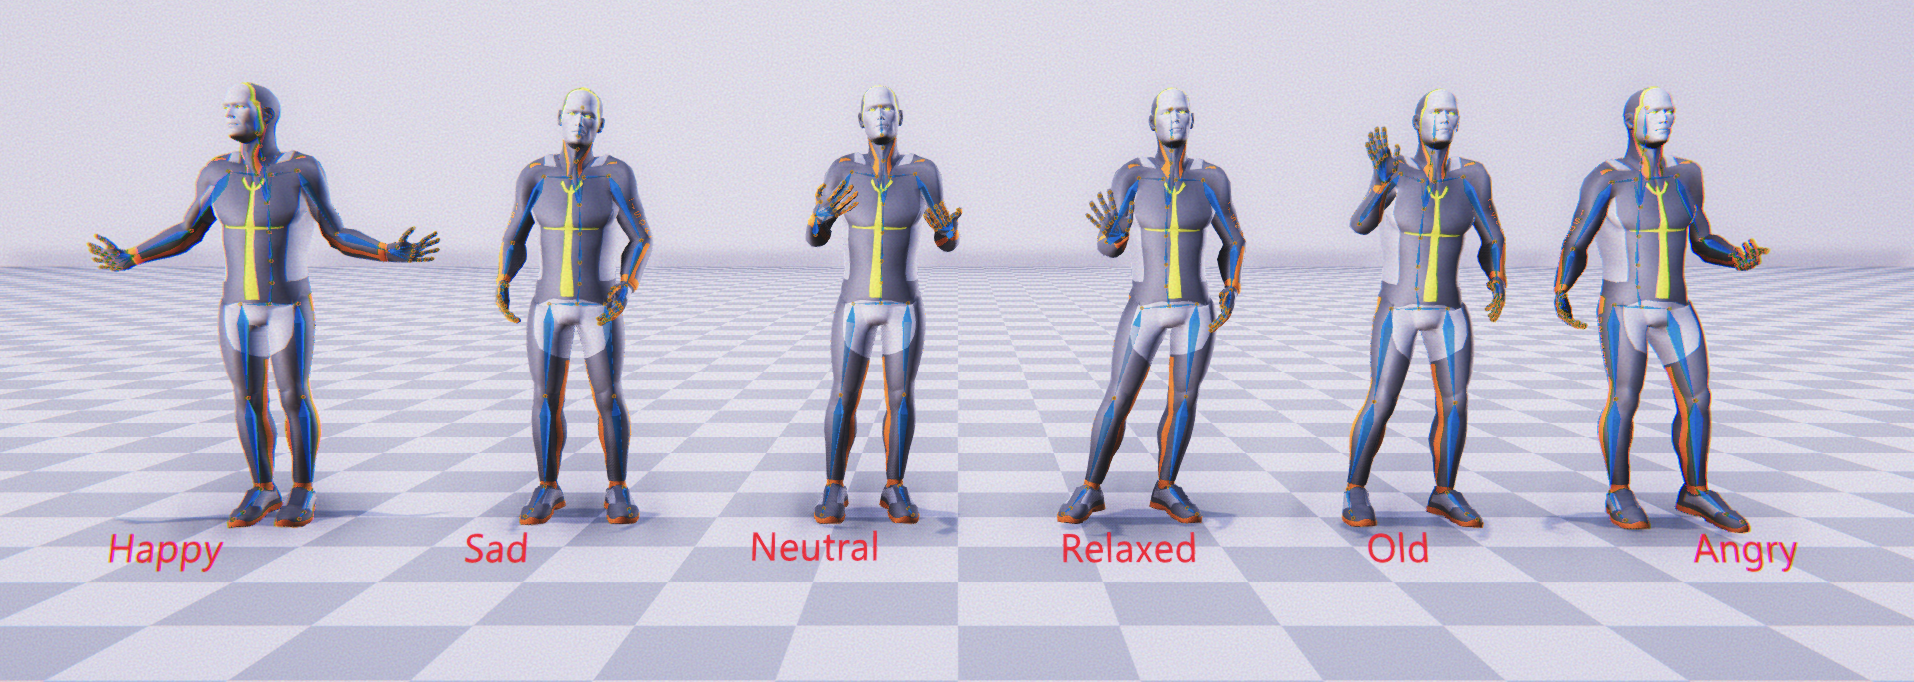
\includegraphics[width=\textwidth]{EmotionAnimation}
	\caption{Minh họavề 6 cử chỉ $\texttt{Happy}$, $\texttt{Sad}$, $\texttt{Neutral}$, $\texttt{Old}$, $\texttt{Relaxed}$ và $\texttt{Angry}$}
\end{figure}

Luận văn sử dụng tập dữ liệu ZeroEGGS \cite{ghorbani2022zeroeggszeroshotexamplebasedgesture} là một bộ dữ liệu motion capture được xây dựng để nghiên cứu và phát triển các mô hình tạo cử chỉ. Nó bao gồm 67 đoạn độc thoại do diễn viên motion capture nữ thực hiện, với tổng thời gian là 135 phút. Các đoạn hội thoại trong tập dữ liệu được biểu diễn với 6 cảm xúc khác nhau: $\texttt{Happy}$, $\texttt{Sad}$, $\texttt{Neutral}$, $\texttt{Old}$, $\texttt{Relaxed}$ và $\texttt{Angry}$, giúp mô phỏng nhiều trạng thái cảm xúc khác nhau trong cử chỉ và chuyển động cơ thể. ZeroEGGS cung cấp một nền tảng phong phú để nghiên cứu khả năng kết hợp giữa bài nói và cử chỉ động, phục vụ cho việc tạo ra các mô hình có thể điều chỉnh cử chỉ tương ứng với cảm xúc và ngữ nghĩa của văn bản.

\section{Công đoạn tiền xử lý dữ liệu}
\label{sec:Preprocessing}

Trong công đoạn {1. Tiền xử lý dữ liệu} (\autoref{fig:CommonStage}), các dữ liệu về cử chỉ, giọng nói, văn bản được đọc và xử lý để biểu diễn thành các vector hoặc ma trận thể hiện thông tin về dữ liệu thô.

Đối với \textbf{dữ liệu văn bản}: Luận văn sử dụng thư viện $\texttt{nltk}$ tách các từ, sử dụng $\texttt{contractions}$ để chuyển các từ viết tắt về dạng chuẩn hóa.

Một trong những đóng góp của luận văn là từ dữ liệu giọng nói có sẵn từ tập ZeroEEGS, luận văn đã sử dụng Adobe Speech To Text để chuyển giọng nói thành văn bản, dùng Montreal Forced Aligner \cite{saxon2020robust} của từ điển âm vị Tiếng Anh để căn chỉnh được thời gian tương ứng với số frame của cử chỉ để thu được các TextGrid. Trong TextGrid sẽ có thời gian tương ứng với từng từ, dựa trên thông tin này, luận văn sử dụng  $\texttt{gensim}$ để nhúng vector word2vec.
 

\textbf{Dữ liệu cử chỉ} bao gồm các tệp BVH (BioVision Motion Capture) được thu nhận từ các cảm biến bằng các hệ thống Motion Capture. Trong các tệp BVH, có chứa hai thành phần gồm Hierachy và Motion. Trong đó:

\begin{itemize}
	\item \texttt{HIERARCHY}: là một cây định nghĩa thông tin khung xương bao gồm 75 bone $\{ \mathbf{b}_1, \mathbf{b}_2 \cdots \mathbf{b}_{75} \} $, mỗi bone bao gồm thông tin về vị trí ban đầu (\texttt{OFFSET}), và các loại tham số \texttt{CHANNELS} thể hiện thông tin về loại, thứ tự của góc quay (\texttt{Zrotation}, \texttt{Yrotation} \texttt{Xrotation}) và vị trí (\texttt{Xposition}, \texttt{Yposition}, \texttt{Zposition}) sẽ định nghĩa trong phần \texttt{MOTION}. Bone (thường là \texttt{Hips}) đầu tiên sẽ là bone gốc $\mathbf{b}_{\text{root}}$, là vị trí sau đó sẽ được forward kinematic (động học thuận) để được T-Shape là ví trí ban đầu của toàn bộ khung xương trước khi áp dụng chuyển động.
	
	\item \texttt{MOTION}: là chuỗi các khung hình. Mỗi khung hình là dữ liệu chuyển động thể hiện sự thay đổi của toàn bộ $75$ khung xương đã định nghĩa trong \texttt{CHANNELS} của \texttt{HIERARCHY}.
\end{itemize}


Mô hình của luận văn chuyển dữ liệu từ góc quay Euler sang góc quay Quaternion, với góc quay Quaternion là một véc-tơ gồm 4 phần tử.

\begin{equation} \label{eq:gesturevector}
	\mathbf{g} = \Big[ \mathbf{p}_{\text{root}},  \mathbf{r}_{\text{root}},
	\mathbf{ p }'_{\text{root}},  \mathbf{r}'_{\text{root}},
	\mathbf{p}_{\text{joins}},  \mathbf{r}_{\text{joins}},
	\mathbf{p}'_{\text{joins}},  \mathbf{r}'_{\text{joins}},
	\mathbf{d}_{\text{gaze}}
	\Big]
\end{equation}

Trong  đó với mỗi $\mathbf{g} \in \mathbb{R}^{1141}$ bao gồm:
{
	\begin{itemize}
		\item $\mathbf{p}_{\text{root}} \in \mathbb{R}^3$: tọa độ của điểm gốc
		\item $\mathbf{r}_{\text{root}} \in \mathbb{R}^4$: Góc quay của điểm gốc
		\item $\mathbf{p}'_{\text{root}} \in \mathbb{R}^3$: Vận tốc thay đổi của tọa độ gốc
		\item $\mathbf{r}'_{\text{root}} \in \mathbb{R}^3$: Vận tốc thay đổi của góc quay gốc
		
		\item $\mathbf{p}_{\text{joins}} \in \mathbb{R}^{3 n_{\text{join} }}$: tọa độ của các khung xương
		\item $\mathbf{r}_{\text{joins}} \in \mathbb{R}^{6 n_{\text{join} }}$: Góc quay của các khung xương theo mặt phẳng X và Y
		\item $\mathbf{p}'_{\text{joins}} \in \mathbb{R}^{3n_{\text{join} }}$: Vận tốc thay đổi của tọa độ các khung xương
		\item $\mathbf{r}'_{\text{joins}} \in \mathbb{R}^{3n_{\text{join} }}$: Vận tốc thay đổi của góc quay các khung xương
		\item $\mathbf{d}_{\text{gaze}} \in \mathbb{R}^3$: Là hướng nhìn
\end{itemize}}

Chuỗi cử chỉ ban đầu có dữ liệu là góc quay sẽ được chuyển thành các góc quay radian, từ góc quay radian ở dạng Euler sẽ được chuyển sang góc quay Quaternion, với quá trình cụ thể được trình bày trong \autoref{appendix:BVHData:QuaternionConvert}.

\textbf{Dữ liệu giọng nói}: $\mathbf{a}_{\text{raw}} \in \mathbb{R}^{ \text{length } }$ là chuỗi giọng nói thô được đọc ở sample rate 16000, sau đó được cắt thành $\mathbf{a} \in \mathbb{R}^{64000}$ tương ứng với 4 giây. Luận văn sử dụng thư viện \texttt{ffmpeg-normalize} để chuẩn hóa tiếng nói nhỏ hơn so với giọng nói gốc.

\textbf{Cảm xúc}: Dữ liệu cảm xúc sẽ được biểu diễn bằng một vector one-hot encoding sẵn. Trong quá trình lấy mẫu, tên tệp sẽ định nghĩa luôn thông tin về cảm xúc mong muốn.

Toàn bộ dữ liệu sẽ được lưu bằng $\texttt{h5}$ được dùng để lưu trữ dữ liệu.

\section{Quá trình huấn luyện}

Toàn bộ quá trình huấn luyện mô hình được thực hiện trong vòng 1 ngày với các tham số sau: số bước huấn luyện $T = 1000$, sử dụng GPU Nvidia 3090, và chia tập dữ liệu theo tỷ lệ $8:1:1$ cho các tập training, testing và validation. Learning rate được thiết lập là $3 \times 10^{-5}$, với batch size là $640$ và tổng cộng $43,853$ mẫu. 
$\gamma = 0.1$.

$\beta$ bắt đầu từ $0.5 \rightarrow 0.999$

Quá trình huấn luyện được triển khai trên mã nguồn công khai tại: \hyperlink{https://github.com/hmthanh/OHGesture}{Github/OHGesture} \footnote{\url{https://github.com/hmthanh/OHGesture}}.


\section{Quá trình sử dụng Unity để kết xuất}
\label{sec:Render}

Để trực quan hóa quá trình sinh cử chỉ từ dữ liệu đầu ra của mô hình, trong công đoạn \textit{7. Kết xuất} (\autoref{fig:CommonStage}) luận văn sử dụng Unity, kế thừa mã nguồn từ mô hình DeepPhase \cite{starke2022deepphase}  . Dữ liệu sau khi sinh là tệp BVH (BioVision Motion Capture). Trong Unity, luận văn bổ sung mã nguồn C-Sharp để kết xuất theo vị trí tọa độ và nhãn tương ứng, với vị trí và góc quay của các xương được biểu diễn dưới dạng quaternion.

Chi tiết phần render cử chỉ được sinh ra, tôi trình bày ở \autoref{Appendix3}.

Mã nguồn chương trình Unity được luận văn công khai ở \hyperlink{https://github.com/DeepGesture/deepgesture-unity}{Github/DeepGesture-Unity}
\footnote{\url{https://github.com/DeepGesture/deepgesture-unity}}.



\chapter{KẾT QUẢ VÀ ĐÁNH GIÁ}
\label{chap:evalution}

\section{Phương pháp đánh giá}

Quá trình đánh giá được thực hiện qua hai độ đo chính là: Mean Opinion Scores (MOS) và Fréchet Inception Distance (FID).

\subsection{Mean Opinion Scores (MOS)}

Hiện tại, chưa có một độ đo chung cho bài toán sinh cử chỉ, đặc biệt là sinh cử chỉ từ giọng nói, vì vậy luận văn dựa vào đánh giá chủ quan của con người để thực hiện các đánh giá thực nghiệm. 
Tương tự như các phương pháp trước đây \cite{yoon2022genea}; \cite{kucherenko2021large}; các mô hình sinh cử chỉ điều khiển bằng giọng nói vẫn thiếu các chỉ số mục tiêu phản ánh một cách nhất quán với nhận thức chủ quan của con người  \cite{alexanderson2022listen}.
MOS được đo lường thông qua ba tiêu chí:

\begin{itemize}
	\item Human-likeness (Mức độ giống con người)
	\item Gesture-Speech Appropriateness (Sự phù hợp giữa cử chỉ và giọng nói)
	\item Gesture-style Appropriateness (Sự phù hợp giữa phong cách cử chỉ)
\end{itemize}


\subsection{Fréchet Inception Distance (FID)}
FID đo sự tương đồng về phân phối giữa cử chỉ sinh ra $\mathbf{g}$ và cử chỉ thực tế $\mathbf{r}$. Công thức tính FID là:

\begin{equation}
	\text{FID} = \left\| \mu_r - \mu_g \right\|^2 + \operatorname{Tr}\left( \Sigma_r + \Sigma_g - 2 \sqrt{\Sigma_r \Sigma_g} \right)
	\label{eq:fidscore}
\end{equation}


%\begin{itemize}
%	\item $\mu_r$ và $\Sigma_r$ là vector trung bình và ma trận hiệp phương sai của đặc trưng từ dữ liệu thực tế (real gestures).
%	\item $\mu_g$ và $\Sigma_g$ là vector trung bình và ma trận hiệp phương sai của đặc trưng từ cử chỉ tổng hợp (generated gestures).
%	\item $\|\mu_r - \mu_g\|^2$ là bình phương khoảng cách Euclidean giữa các vector trung bình.
%	\item $\text{Tr}\left( \Sigma_r + \Sigma_g - 2\sqrt{\Sigma_r \Sigma_g} \right)$ là trace của ma trận hiệp phương sai kết hợp, đo lường sự khác biệt giữa hai phân phối Gaussian.
%\end{itemize}

Trong đó:

\begin{itemize}
	\item $\mu$: Trung bình các đặc trưng của cử chỉ.
	\item $\Sigma$: Ma trận hiệp phương sai của đặc trưng.
	\item $\operatorname{Tr}$: Tổng đường chéo chính của ma trận hiệp phương sai.
	\item $\sqrt{\Sigma_r \Sigma_g}$: Sự tương đồng giữa các phân phối cử chỉ thực tế và cử chỉ sinh ra.
\end{itemize}

FID thấp cho thấy phân phối của cử chỉ sinh ra gần giống với cử chỉ thực tế, trong khi FID cao gợi ý sự khác biệt lớn, cho thấy chất lượng cử chỉ sinh ra kém hơn.





%\begin{itemize}
	%		\item \textbf{FID thấp}: Cho thấy phân phối của cử chỉ sinh ra rất gần với phân phối của cử chỉ thực tế, tức là cử chỉ tổng hợp trông tự nhiên hơn.
	%		\item \textbf{FID cao}: Gợi ý rằng các cử chỉ sinh ra khác biệt nhiều so với các cử chỉ thực tế, tức là chất lượng kém hơn.
	%	\end{itemize}
%	




% ngay cả với Fréchet gesture distance (FGD) \cite{yoon2022genea}, \cite{dabral2023mofusion}. Vì vậy, tất cả các điểm số thực nghiệm trong nghiên cứu này được thực hiện thông qua đánh giá chủ quan của con người. Chúng tôi đánh giá trên ba tiêu chí: độ giống con người, sự phù hợp giữa cử chỉ và giọng nói, và sự phù hợp giữa cử chỉ và phong cách. Các tiêu chí này được lấy từ đánh giá trong GENEA \cite{yoon2022genea}.


%Chúng tôi so sánh mô hình đề xuất của luận văn với StyleGestures \cite{alexanderson2020style}, Audio2Gestures \cite{li2021audio2gestures}, ExampleGestures \cite{ghorbani2022zeroeggszeroshotexamplebasedgesture}.

\section{Kết quả đánh giá}
\label{sec:result}

\subsection{Kết quả đánh giá bằng MSE}

Trong luận văn, chuỗi cử chỉ dữ đoán sẽ được đoạn trên $M$ frame. Luận văn sử dụng Mean Square Error trên chuỗi cử chỉ $\mathbf{x}^{[1:M] \times D}$.

\begin{table}[H]
	\centering
	\resizebox{\textwidth}{!}{%
		\begin{tabular}{lcccccc}
			\hline
			\multicolumn{1}{c}{Cảm xúc} & Tự Nhiên & Buồn Bã &  Vui Vẻ  & Thư Giãn & Lớn Tuổi & Giận Dữ \\ \hline
			DiffuseStyleGesture  & 75.04 & 51.40 & 110.18 & 130.83     & 116.03    & 78.53     \\
			ZeroEGG & 136.33 & 81.22 & 290.47 & 140.24     & 102.44    & 181.07     \\
			\hline
			Mô hình đề xuất                     &         &         &         &           &          &                 \\
			\quad \textbf{OHGesture} & 161.22 & 89.58 & 279.95 & 156.93   & 99.86   & 215.24    \\
			\hline
		\end{tabular}%
	}
	\caption{Kết quả đánh giá Mean Square Error theo 6 cảm xúc}
	\label{table:EvaluationMSE}
\end{table}

\subsection{Kết quả đánh giá bằng MOS}

Ở đây luận văn sử dụng lại kết quả đánh giá của mô hình baseline \textbf{DiffuseStyleGesture} \cite{yang2023diffusestylegesture} trong độ đo về  cảm nhận đánh giá của con người do lĩnh vực sinh cử chỉ vẫn còn rất mới, chi phí để ước lượng các mô hình còn lớn nên luận văn không thể đánh giá được mô hình OHGesture. Vì vậy các kết quả này chưa bao gồm thông tin kết qủa về mô hình \textbf{OHGesture} mà luận văn đề xuất.

\begin{figure}[htbp]
	\centering
	\begin{subfigure}[b]{0.3\textwidth}
		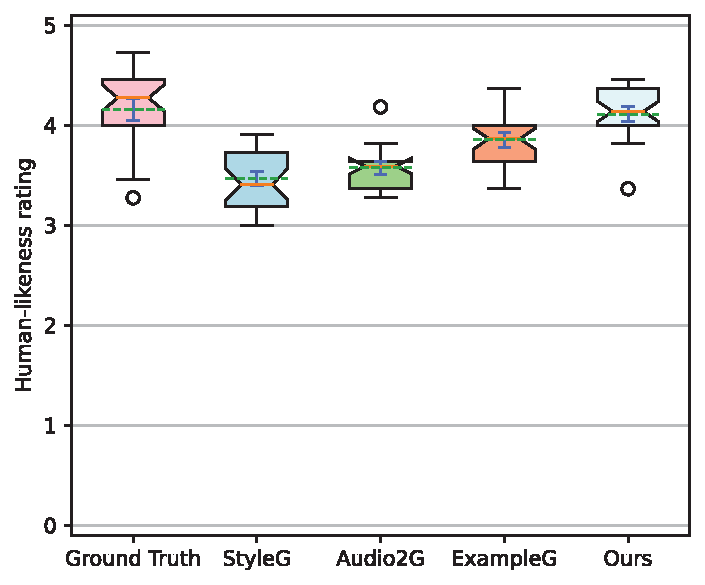
\includegraphics[width=\textwidth]{BoxHumanLikeness.pdf}
		\caption*{(a) Human-likeness}
	\end{subfigure}
	\hfill
	\begin{subfigure}[b]{0.3\textwidth}
		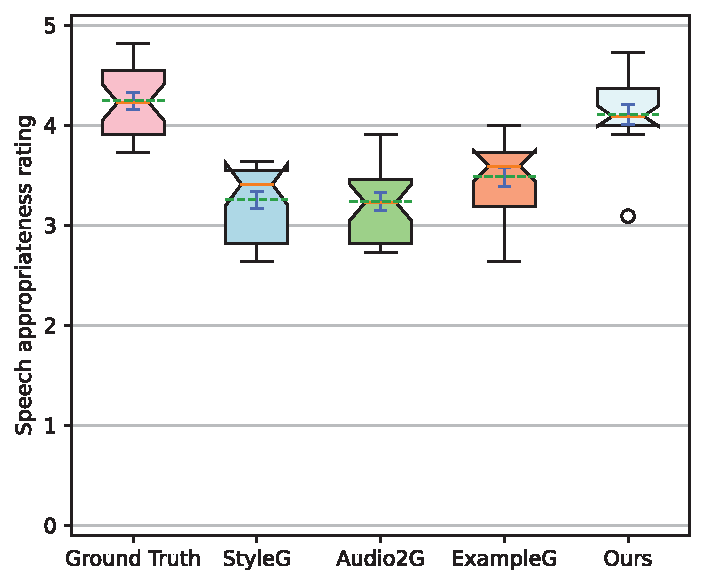
\includegraphics[width=\textwidth]{BoxSpeechAppropriateness.pdf}
		\caption*{\small (b) Speech Appropriateness}
	\end{subfigure}
	\hfill
	\begin{subfigure}[b]{0.3\textwidth}
		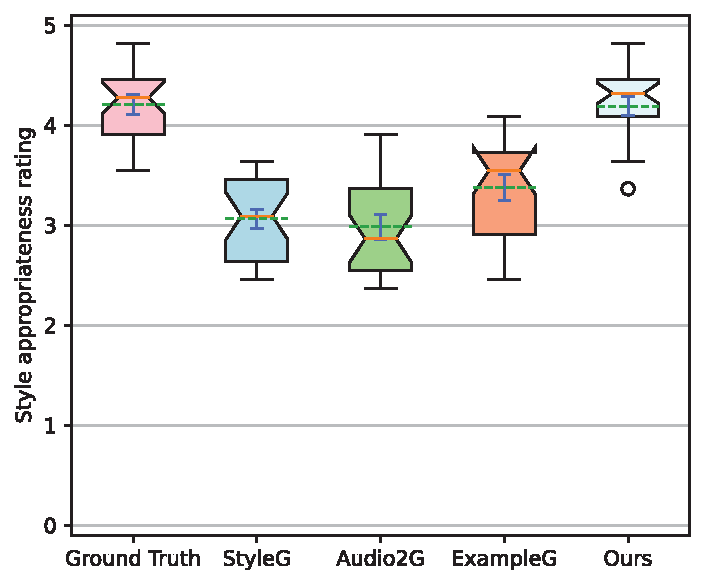
\includegraphics[width=\textwidth]{BoxStyleAppropriateness.pdf}
		\caption*{(c) Style Appropriateness}
	\end{subfigure}
	
	%	    \caption[Biểu đồ hộp mô tả kết quả so sánh MOS]{Biểu đồ hộp mô tả kết quả so sánh MOS cho các mô hình khác nhau trong các chiều khác nhau. Hộp mở rộng từ phân vị thứ nhất thấp nhất (Q1) đến phân vị thứ ba lớn nhất (Q3) của dữ liệu. Đường đỏ chỉ là giữa. Các khe nhỏ biểu thị khoảng tin cậy $95\%$ (CI) xung quanh giữa. Khi CI nhỏ hơn Q1 hoặc lớn hơn Q3, khe mở rộng ra khỏi hộp, tạo ra một hình dáng "lật" độc đáo. Chúng tôi cũng đã đánh dấu giá trị trung bình và khoảng tin cậy $95\%$ của nó trong hình với đường nét đứt màu xanh lá cây và đường dọc màu xanh lam, tương ứng.}
	\label{fig:compare }
\end{figure}


Để hiểu hiệu suất thị giác thực tế của phương pháp của luận văn, luận văn tiến hành một nghiên cứu người dùng so sánh các cử chỉ được tạo ra từ phương pháp của luận văn và dữ liệu chụp chuyển động thực tế. Độ dài của các đoạn clip đánh giá dao động từ 11 đến 51 giây, với độ dài trung bình là 31.6 giây, dài hơn so với các đoạn trong đánh giá GENEA \cite{yoon2022genea} (8-10 giây), vì thời gian dài hơn có thể tạo ra kết quả rõ ràng và thuyết phục hơn \cite{yang2022reprgesture}. Người tham gia đánh giá trên thang điểm từ 5 đến 1, với các nhãn từ $\texttt{excellent}$,  $\texttt{good}$, $\texttt{fair}$, $\texttt{poor}$, đến $\texttt{bad}$. 

\begin{table}[H]
	\centering
	\begin{tabular}{lcc}
		\hline
		\multicolumn{1}{c}{Name} &
		\begin{tabular}[c]{@{}c@{}}Human\\ likeness \end{tabular}$\uparrow$ &
		\begin{tabular}[c]{@{}c@{}}Gesture-speech\\ appropriateness\end{tabular}$\uparrow$ \\ \hline
		Ground Truth          & 4.15 $\pm$ 0.11          & 4.25 $\pm$ 0.09          \\
		Ours                  & \textbf{4.11 $\pm$ 0.08} & \textbf{4.11 $\pm$ 0.10} \\
		\quad$-$ WavLM             & 4.05 $\pm$ 0.10          & 3.91 $\pm$ 0.11          \\
		\quad$-$ Cross-local attention   & 3.76 $\pm$ 0.09          & 3.51 $\pm$ 0.15          \\
		\quad$-$ Self-attention    & 3.55 $\pm$ 0.13          & 3.08 $\pm$ 0.10          \\
		\quad$-$ Attention + GRU&
		3.10 $\pm$ 0.11 &
		2.98 $\pm$ 0.14 \\
		\quad$+$ Forward attention & 3.75 $\pm$ 0.15          & 3.23 $\pm$ 0.24          \\
		\hline
	\end{tabular}
	\caption{Kết quả đánh giá bằng MOS trên Genea (năm 2022)}
	\label{table:MOSScore}
\end{table}
%Kết quả của các nghiên cứu loại bỏ (Ablation studies). "$-$" chỉ các mô-đun không được sử dụng và "$+$" chỉ các mô-đun bổ sung. Chữ in đậm chỉ ra chỉ số tốt nhất

\subsection{Kết quả đánh giá bằng FGD}

Luận văn đề xuất Fréchet Gesture Distance (FGD), hệ số FID dựa trên cử chỉ (gesture), và xây dựng mã nguồn \hyperlink{https://github.com/GestureScore/GestureScore}{GestureScore} \footnote{Github/GestureScore: \url{https://github.com/GestureScore/GestureScore}} . Trong GestureScore, luận văn xây dựng một Inception V3 model, để mã hoá chuỗi khung hình $\bx^{1:M \times D}$ thành vector tiềm ẩn kích thước $32 \times 32$. Sử dụng vector này làm đầu vào cho \autoref{eq:fidscore}. Sau đây là \autoref{table:EvalFGD} đánh giá kết quả của mô hình OHGesture bằng GestureScore

%$\uparrow$
\begin{table}[H]
	\centering
	\begin{tabular}{lcc}
		\hline
		\multicolumn{1}{c}{Name} & FGD trên vector đặc trưng & \begin{tabular}[c]{@{}c@{}} FGD dữ liệu gốc \end{tabular} \\ \hline
		Ground Truth             & -       & -          \\
		Ours                     &       & \\
		\quad OHGesture (Feature D=1141) & 2.058      & 9465.546 \\
		\quad OHGesture (Rotations) & 3.513       & 9519.129 \\
		\hline
		
	\end{tabular}
	\caption{Kết quả đánh giá Fréchet Gesture Distance (FGD) trên $\bx^{1:M \times D}$ (từ frame 1 đến frame M, mỗi frame có D đặc trưng từng khung hình )}
	%	\caption{Kết quả của các nghiên cứu loại bỏ (Ablation studies). "$-$" chỉ các mô-đun không được sử dụng và "$+$" chỉ các mô-đun bổ sung. Chữ in đậm chỉ ra chỉ số tốt nhất.}
		\label{table:EvalFGD}
\end{table}

\begin{itemize}[]
		\item \textbf{Vector đặc trưng}
	Sử dụng tệp BVH để chuyển toàn bộ skeleton của mỗi khung hình thành vector đặc trưng $D = 1141 $ như công thức  \autoref{eq:gesturevector}
	
	\item  \textbf{Rotations}: Từ tệp BVH kết quả, luận văn trích xuất sự thay đổi của các góc quay (rotations), $D = 225$ ($225 = 75 \times 3$) của chuỗi cử chỉ với chiều dài mỗi đoạn là $M$ frame để đánh giá ở dòng OHGesture bên dưới. 
	
\end{itemize}

\section{Xây dựng và tiêu chuẩn hóa hệ thống đánh giá kết quả sinh cử chỉ}

Hiện nay các mô hình sinh (gesture generation) cử chỉ được quan tâm nghiên cứu với rất nhiều mô hình khác nhau, tuy nhiên do không có độ đo chung, vì các độ đo truyền thống như FID (Fréchet Inception Distance) hay IS (Inception Score),.. không thể hiện được hết các tính chất Giống người (Human-likeness), tính phù hợp với giọng nói (Speech Appropriateness), và tính phù hợp với phong cách (Style Appropriateness) của cử chỉ. Các mô hình cũng được thực hiện và huấn luyện trên một tập dữ liệu khác nhau, vì vậy rất khó để biết được mô hình nào đã đạt kết quả tốt hơn, và mô hình nào là mô hình state-of-the-art, từ đó khó có thể đạt được sự tiến bộ trong lĩnh vực sinh cử chỉ. Việc thiếu tiêu chuẩn chung để đánh giá trong cộng đồng nghiên cứu khiến luận văn mong muốn xây dựng một hệ thống xếp hạng trực tuyến \cite{nagy2024towards} \hyperlink{https://genea-workshop.github.io/leaderboard/}{GENEA Leaderboard} \footnote{GENEA Leaderboard: \url{https://genea-workshop.github.io/leaderboard/}}., là một bảng xếp hạng các mô hình sinh cử chỉ. Luận văn thu thập và xử lý một tập dữ liệu cử chỉ từ nhiều ngôn ngữ và từ nhiều tập dữ liệu khác nhau và tiêu chuẩn hóa để tạo ra một tập dữ liệu duy nhất.  Sau đó, luận văn sẽ mời các tác giả của các mô hình để học và dự đoán trên tập dữ liệu đã được tiêu chuẩn hóa, sau khi có kết quả sinh cử chỉ, luận văn sẽ thuê những người tham gia nghiên cứu trên Prolific để đánh giá và xếp hạng kết quả sinh cử chỉ của các mô hình. Hiện tại luận văn đang xây dựng hệ thống trực tuyến \hyperlink{https://github.com/hemvip/hemvip.github.io}{hemvip/hemvip.github.io}\footnote{HEMVIP2 \url{https://github.com/hemvip/hemvip.github.io}} với mục tiêu đánh giá kết quả sinh của cử chỉ thông qua việc thuê các người tham gia đánh giá kết quả thông qua Prolific. Luận văn sẽ bổ sung các đánh giá về mô hình OHGesture dựa trên các điểm số trên.


Thông qua hệ thống đánh giá này, nghiên cứu kỳ vọng sẽ thiết lập một tiêu chuẩn chung, từ đó tạo động lực cho sự tiến bộ trong lĩnh vực sinh cử chỉ.

%Chi tiết về nghiên cứu người dùng có thể được tìm thấy trong tư liệu bổ sung.

%Điểm số ý kiến trung bình (MOS) về độ giống con người, sự phù hợp giữa cử chỉ và giọng nói, và sự phù hợp giữa cử chỉ và phong cách được báo cáo trong \ref{fig}. 
%Nếu các góc của hai hộp không chồng lên nhau, điều này chứng tỏ rằng các phân phối khác biệt đáng kể \cite{mcgill1978variations}. Phương pháp của luận văn vượt trội so với các phương pháp tiên tiến được so sánh trong cả ba chiều đánh giá, và thậm chí tạo ra các kết quả cạnh tranh với dữ liệu thực tế. Phản hồi từ người tham gia cho thấy cử chỉ do phương pháp của luận văn tạo ra "có ý nghĩa ngữ nghĩa hơn", "tự nhiên hơn", và "phù hợp với phong cách", mặc dù có một số vấn đề về "chuyển động trượt chân" so với Dữ liệu Thực. Tuy nhiên, đây là một vấn đề phổ biến đối với các hệ thống tạo ra chuyển động không dựa trên vật lý và có thể được giải quyết thông qua xử lý sau \cite{ghorbani2022zeroeggszeroshotexamplebasedgesture}, \cite{luvizon2023scene}.

%Hiện tại chưa có một độ đo chung cho bài toán sinh cử chỉ, đặc biệt là sinh cử chỉ từ giọng nói, vì vậy luận văn 
%các cử chỉ điều khiển bằng giọng nói thiếu các chỉ số mục tiêu phản ánh một cách nhất quán với nhận thức chủ quan của con người \cite{yoon2022genea}; \cite{kucherenko2021large}; \cite{alexanderson2022listen}, ngay cả với Fréchet gesture distance (FGD) \cite{yoon2022genea}, \cite{dabral2023mofusion}, do đó tất cả các điểm số thực nghiệm của luận văn được thực hiện thông qua đánh giá chủ quan của con người. Chúng tôi thực hiện đánh giá trên ba chiều. Hai chiều đầu tiên theo đánh giá trong GENEA \cite{yoon2022genea}, bao gồm đánh giá về độ giống con người và sự phù hợp giữa cử chỉ và giọng nói. Chiều thứ ba là sự phù hợp giữa cử chỉ và phong cách.
%
%Nghiên cứu Người Dùng. Để hiểu về hiệu suất thị giác thực tế của phương pháp của luận văn, luận văn tiến hành một nghiên cứu người dùng giữa các trình tự cử chỉ được tạo ra bởi mỗi phương pháp được so sánh và dữ liệu chụp chuyển động thực. Độ dài của các đoạn clip được đánh giá dao động từ 11 đến 51 giây, với độ dài trung bình là 31.6 giây. Lưu ý rằng các cử chỉ clip được sử dụng cho đánh giá chủ quan ở đây dài hơn so với đánh giá GENEA \cite{yoon2022genea} (8-10 giây), vì một khoảng thời gian dài có thể tạo ra kết quả phù hợp rõ ràng và thuyết phục hơn \cite{yang2022reprgesture}. Người tham gia đánh giá trên một khoảng điểm từ 5 đến 1, với các nhãn (tốt nhất đến tệ nhất) là "tuyệt vời," "tốt," "công bằng," "kém," và "tệ." Thêm chi tiết về nghiên cứu người dùng được hiển thị trong tư liệu bổ sung.
%
%
%
%
%
%
%Điểm số ý kiến trung bình (MOS) về độ giống con người, phù hợp giọng nói và phù hợp phong cách được báo cáo trong \ref{fig:mosscore}. Nếu các góc của hai hộp không chồng lên nhau, chúng ta có thể coi đây là bằng chứng mạnh mẽ rằng các phân phối khác nhau đáng kể \cite{mcgill1978variations}. Phương pháp của luận văn vượt trội đáng kể so với các phương pháp tiên tiến được so sánh với độ giống con người, phù hợp giữa cử chỉ và giọng nói, cũng như phù hợp giữa cử chỉ và phong cách, và thậm chí tạo ra các kết quả cạnh tranh với dữ liệu thực tế ở cả ba chiều. Theo phản hồi từ người tham gia, cử chỉ được tạo ra bởi luận văn "có ý nghĩa ngữ nghĩa hơn", "tự nhiên hơn," và "phù hợp với phong cách," trong khi phương pháp của luận văn có "chuyển động trượt chân" so với Dữ liệu Thực. Tuy nhiên, đây là một vấn đề phổ biến đối với các hệ thống tạo ra chuyển động không dựa trên vật lý và có thể được giải quyết thông qua xử lý sau \cite{ghorbani2022zeroeggszeroshotexamplebasedgesture}, \cite{luvizon2023scene}.

%\begin{table}[t]
%	\centering
%	\caption{Impact of the positional encoding block.}
%	\label{tab:pos_enc}
%	
%	\newcolumntype{Y}{>{\raggedleft\arraybackslash}X}
%	\newcolumntype{Z}{>{\centering\arraybackslash}X}
%%	\begin{tabularx}{\linewidth}{XlYY}
%	
%%		
%	
%%		\bottomrule
%%		\begin{tabularx}{\linewidth}{XlYY}
%%		\toprule
%%		Dataset & System & FGD $\downarrow$ & PMB ($\%$) $\uparrow$ \\
%%		\toprule
%%		\multirow{2}{*}{TED} & Without positional encoding & 2.19 & 88.13 \\
%%		& With positional encoding & $\bm{2.04}$ & $\bm{89.52}$ \\
%%		\bottomrule
%%		\end{tabularx}
%
%
%
%
%% \begin{tabularx}{\linewidth}{XlYY}
%%	\toprule
%%	Dataset & System & FGD $\downarrow$ & PMB ($\%$) $\uparrow$ \\
%%	\toprule
%%	\multirow{2}{*}{TED} & encoding & 2.19 & 88.13 \\
%%	& With positional encoding & $2.04$ & $89.52$ \\
%%	\bottomrule
%%\end{tabularx}
%
%
%
%%		\multirow{2}*{Trinity} & Without positional encoding & 11.15 & 89.98 \\
%%				& With positional encoding & $\bm{10.78}$ & $\bm{91.36}$ \\
%%\hline
%%This is a long entry that will automatically adjust its width. & Short text & Another long entry that will also adjust its width. \\
%%\hline
%%More text & Another short entry & Yet another long entry to demonstrate text wrapping and width adjustment. \\
%%\hline
%
%\end{table}



% \section{Đánh Giá}
% \label{sec:experiments}
 % Khả năng Kiểm soát Cử chỉ

%\subsection{Khả năng kiểm soát cử chỉ}
%\label{subsec:stylecontrol}

%Giả sử rằng giọng nói trung tính không ảnh hưởng đến phong cách của cử chỉ, chúng ta có thể tạo ra các cử chỉ được phong cách hóa với một bài nói trung tính bằng cách đặt $\gamma=1$ và $e$ trong \ref{eq:denoise}. Chúng tôi chọn hai đoạn hội thoại trong tập kiểm thử với giọng nói trung tính để tạo ra sáu cử chỉ được phong cách hóa tương ứng. \ref{fig:emotiondataset} minh họa cử chỉ được tạo ra $\hat{\mathbf{x}}_{t}$ của các phong cách đầu vào $s$ khác nhau với cùng một giọng nói trung tính được thị giác hóa bằng phương pháp tSNE.
%
%\begin{figure}
%    \centering
%    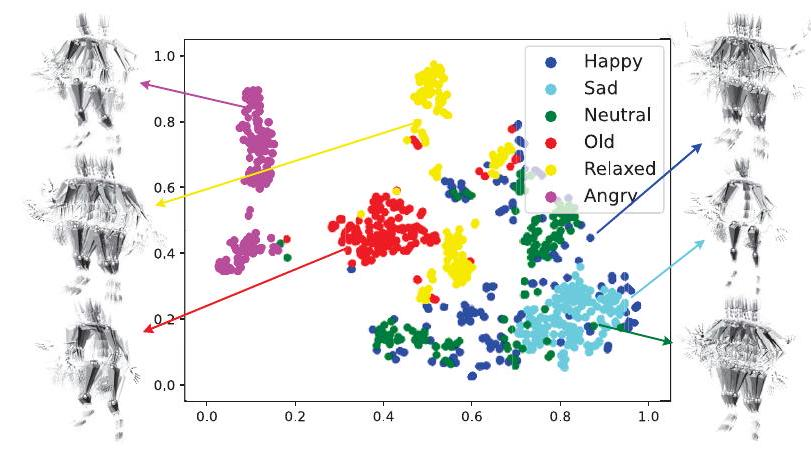
\includegraphics[width=0.7\linewidth]{images/emotion_dataset.jpg}
%    \caption[Biểu đồ tSNE với các phong cách khác nhau]{Hiển thị tSNE của các cử chỉ với các phong cách khác nhau và bản đồ bóng của cử chỉ xương cơ với phong cách tương ứng. Ví dụ, với cử chỉ 'Old', hông và đầu gối của nó uốn cong hơn, và tay của nó cơ bản nằm ở đầu gối hoặc hông.}
%    \label{fig:emotiondataset}
%\end{figure}
%
%Chúng tôi cũng vẽ biểu đồ xương cơ được tạo ra bởi phong cách tương ứng trong hình, và có thể thấy rằng đối với phong cách 'Old', hông và đầu gối của nó uốn cong hơn, và tay của nó cơ bản nằm ở đầu gối hoặc hông; với phong cách 'Sad', đầu của nó đang nghiêng và tay nó ở một vị trí thấp hơn; với phong cách 'Relax', hông của nó đang chuyển lên phía trước và tư thế đứng của nó là thoải mái; với phong cách 'Angry', tay của nó di chuyển lên và xuống nhanh chóng. Lưu ý rằng mặc dù sự khác biệt giữa cử chỉ phong cách 'trung tính' và 'Happy' vẫn khá rõ ràng trong việc thị giác hóa phong cách của xương cơ, tức là với phong cách 'Happy', vị trí tay của nó là cao hơn và biên độ của nó lớn hơn, tuy nhiên tSNE của chúng gần như kết hợp với nhau. Trong phân tích của luận văn, điều này xảy ra vì bài nói trung tính gọi là vẫn chứa thông tin như cảm xúc và ngữ nghĩa mà có trong các đặc trưng WavLM. Sự cân bằng giữa phong cách từ giọng nói $\mathbf{a}$ và từ phong cách $\mathbf{e}$ có thể được kiểm soát thêm bằng cách chỉnh sửa cường độ phong cách $\gamma$.
%
%Giả sử rằng giọng nói Neutral không ảnh hưởng đến cảm xúc của cử chỉ, chúng ta có thể tạo ra các cử chỉ được điều chỉnh theo cảm xúc với một bài nói Neutral bằng cách đặt $\gamma=1$ và $e$ trong \ref{eq:denoise}. Chúng tôi chọn hai đoạn hội thoại trong tập kiểm thử với giọng nói trung tính để tạo ra sáu cử chỉ được điều chỉnh cảm xúc tương ứng. Hình \ref{fig:emotiondataset} minh họa cử chỉ được tạo ra $\hat{\mathbf{x}}_{t}$ cho các cảm xúc đầu vào $s$ khác nhau với cùng một giọng nói trung tính, được thị giác hóa bằng phương pháp t-SNE.
%
%\begin{figure}
%	\centering
%	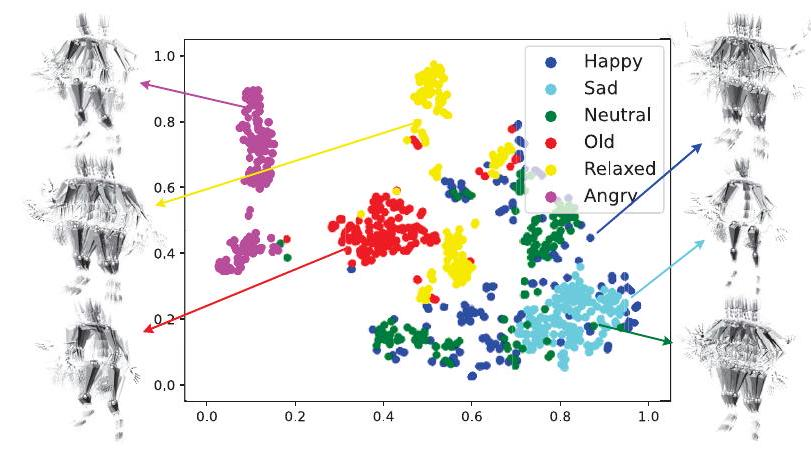
\includegraphics[width=0.7\linewidth]{images/emotion_dataset.jpg}
%	\caption[Biểu đồ t-SNE với các cảm xúc khác nhau]{Hiển thị t-SNE của các cử chỉ với các cảm xúc khác nhau và bản đồ bóng của cử chỉ xương cơ với cảm xúc tương ứng. Ví dụ, với cử chỉ 'Old', hông và đầu gối của nó uốn cong hơn, và tay của nó cơ bản nằm ở gần đầu gối hoặc hông.}
%	\label{fig:emotiondataset}
%\end{figure}
%
%Chúng tôi cũng biểu diễn các cử chỉ khung xương tương ứng với từng cảm xúc trong hình và nhận thấy rằng đối với cảm xúc 'Old', hông và đầu gối có độ uốn cong lớn hơn, và tay chủ yếu nằm ở đầu gối hoặc hông; với cảm xúc 'Sad', đầu nghiêng và tay ở vị trí thấp hơn; với cảm xúc 'Relaxed', hông hơi hướng về phía trước với tư thế đứng thoải mái; với cảm xúc 'Angry', tay chuyển động nhanh chóng lên xuống. Lưu ý rằng mặc dù sự khác biệt giữa cử chỉ với cảm xúc 'Neutral' và 'Happy' vẫn rõ ràng khi thị giác hóa khung xương, cụ thể là với cảm xúc 'Happy', tay ở vị trí cao hơn và biên độ lớn hơn, nhưng các điểm t-SNE của chúng lại gần nhau. Trong phân tích của luận văn, điều này là do bài nói trung tính vẫn chứa thông tin về cảm xúc và ngữ nghĩa từ các đặc trưng của WavLM. Sự cân bằng giữa cảm xúc từ giọng nói $\mathbf{a}$ và từ điều chỉnh cảm xúc $\mathbf{e}$ có thể được kiểm soát thêm thông qua việc điều chỉnh cường độ cảm xúc $\gamma$.



%\subsection{Khả năng điều chỉnh cảm xúc của cử chỉ}
%
%
%\begin{figure}
%	\centering
%	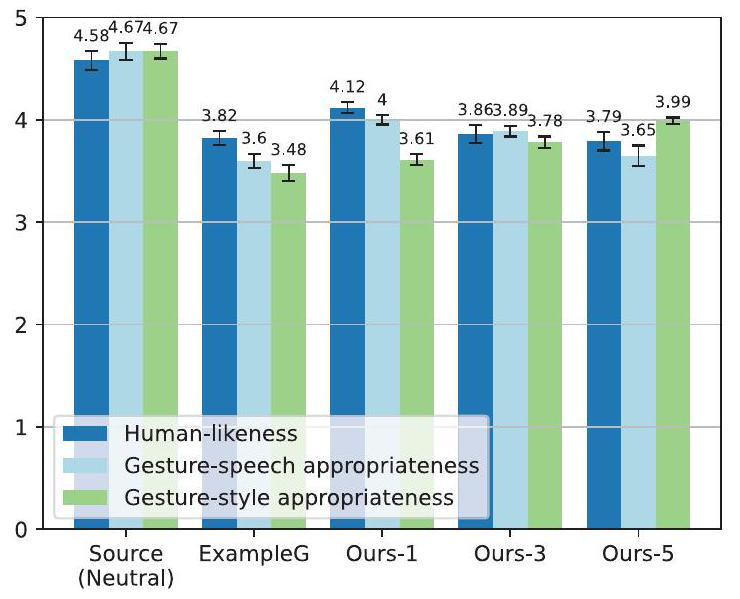
\includegraphics[width=0.7\linewidth]{images/mos_score.jpg}
%	\label{fig:mosscore}
%	\caption{Kết quả trung bình của MOS}
%	
%	%    \caption[Kết quả trung bình của MOS]{Kết quả trung bình của MOS với khoảng tin cậy $95\%$ cho ba chiều. 'Ours-$\gamma$' chỉ ra cường độ kiểm soát phong cách $\gamma$ của mô hình của luận văn. Mô hình của luận văn vượt trội đáng kể so với ExampleGesture tổng thể và có thể chỉnh sửa cường độ của các phong cách. Tham số $\gamma$ tăng và hai điểm số còn lại sẽ giảm một cách hợp lý.}
%	
%	\vspace{-10pt}
%\end{figure}

%Trong nghiên cứu này, luận văn điều chỉnh cường độ cảm xúc của cử chỉ thông qua tham số $\gamma$, với các giá trị $\gamma=1$ và $\gamma=3$ cho cảm xúc 'Happy' và 'Old'. Khi $\gamma=3$, cảm xúc 'Happy' tạo ra cử chỉ mạnh mẽ với chuyển động tay và cơ thể rõ rệt, trong khi 'Old' thể hiện cử chỉ ít năng động hơn, với hông ít uốn cong và tay ít được nâng lên. Các giá trị $\gamma$ khác cho phép điều chỉnh cường độ cảm xúc, giúp tạo ra cử chỉ tương ứng với các cảm xúc chuyển tiếp giữa 'Happy' và 'Old'. Các thử nghiệm cho thấy rằng việc tăng $\gamma$ giúp tạo ra cử chỉ phù hợp với cảm xúc mong muốn, ngay cả khi chúng không có trong dữ liệu huấn luyện. 
%Một nghiên cứu người dùng cho thấy mô hình của luận văn vượt trội so với ExampleGesture trong việc điều chỉnh cường độ cảm xúc và tạo ra cử chỉ tự nhiên và phù hợp với ngôn ngữ.
%
%Để phân tích chi tiết hơn mối quan hệ giữa cường độ cảm xúc và cảm xúc mà bài nói ngụ ý, luận văn lựa chọn hai cảm xúc là 'Happy' và 'Old' và thiết lập $\gamma=1$ và $3$ trong \ref{eq:denoise}. Để so sánh kết quả, luận văn cũng thiết lập $\gamma=0.5$ trong \ref{eq:denoise} để nội suy giữa các cảm xúc khác nhau. Các tham số còn lại được giữ nguyên, và luận văn biểu diễn cử chỉ được tạo ra trong 12 giây với FPS $=1$.
%
%Có thể quan sát thấy rằng khi sử dụng cảm xúc 'Happy' với $\gamma=3$, chuyển động cơ thể và cử động tay đều đạt cường độ cao nhất, và vị trí tay được nâng cao nhất; ngược lại, khi sử dụng cảm xúc 'Old' với $\gamma=3$, hông có độ uốn cong lớn nhất, tay ít được nâng lên, và chuỗi chuyển động nhìn chung có ít thay đổi. Đối với ba kết quả còn lại, cường độ cảm xúc nằm giữa hai trường hợp này, với cảm xúc dần chuyển từ Happy sang Old. Kiến trúc mô hình của luận văn giúp cử chỉ và bài nói kết hợp với nhau hài hòa hơn, dù hai cảm xúc không hoàn toàn giống nhau. Lưu ý rằng khi sử dụng cảm xúc 'Happy' và 'Old' với $\gamma=0.5$, kết quả gần giống như khi sử dụng cảm xúc 'Happy' với $\gamma=1$, trong khi cảm xúc 'Old' khó nhận ra. Quan sát này khẳng định kết luận trước đó rằng cảm xúc 'Happy' đã được thể hiện trong bài nói 'Neutral' dùng để kiểm thử. Điều này cho thấy, chẳng hạn, trong các thử nghiệm của luận văn, nếu muốn điều chỉnh bài nói 'Happy' để tạo ra cử chỉ 'Sad', $\gamma=1$ có thể không hiệu quả do mô hình có xu hướng học cảm xúc Happy từ bài nói. Do sự tương quan giữa cảm xúc của bài nói và cảm xúc của cử chỉ, việc tăng giá trị $\gamma$ có thể giúp điều chỉnh cảm xúc tốt hơn, cho phép tạo ra các cử chỉ không có trong tập dữ liệu gốc (ví dụ: cử chỉ cho bài nói 'Happy' nhưng có cảm xúc 'Sad') thông qua việc điều chỉnh cường độ cảm xúc.
%
%Hơn nữa, để tìm hiểu mối quan hệ giữa cường độ cảm xúc với độ giống con người (human-likeness) và sự phù hợp với ngôn ngữ, luận văn đã tiến hành một nghiên cứu người dùng. Để tránh ảnh hưởng của cảm xúc trong ngôn ngữ nói đến đánh giá của người tham gia, tương tự như trước, luận văn chỉ điều chỉnh cường độ cảm xúc cho một bài nói Neutral và yêu cầu người tham gia đánh giá theo ba tiêu chí đặc trưng trước đó. ExampleGesture \cite{ghorbani2022zeroeggszeroshotexamplebasedgesture} cũng cho phép kiểm soát việc tạo ra các cảm xúc khác nhau từ cùng một bài nói, vì vậy luận văn chọn nó làm mô hình tham chiếu. Do các cử chỉ được tạo ra ở đây không tồn tại trong tập dữ liệu, bài nói Neutral với cảm xúc trung tính được sử dụng làm tham chiếu.

%
%\subsection{Khả năng chỉnh sửa Phong cách của cử chỉ}
%
%Để phân tích sâu hơn mối quan hệ giữa cường độ phong cách và phong cách được ngụ ý bởi bài nói, luận văn chọn phong cách 'Happy' và phong cách 'Old' và đặt $\gamma=1$ và 3 trong \ref{eq:denoise}. Ngoài ra, để so sánh kết quả, luận văn đặt $\gamma=0.5$ trong \ref{eq:denoise}, để nội suy giữa các phong cách khác nhau. Các tham số khác không thay đổi, và luận văn vẽ kết quả tạo ra cử chỉ trong 12 giây, với FPS $=1$.
%%như thể hiện trong 
%%\ref{fig:stylesample}.
%
%
%%Như thấy trong
%% \ref{fig:stylesample}, 
% Chúng ta có thể thấy rằng khi chúng ta sử dụng phong cách 'Happy' với $\gamma=3$, cả quá trình xoay cơ thể và chuyển động tay đều lớn nhất, và vị trí tay của nó là cao nhất; ngược lại, khi chúng ta sử dụng phong cách 'Old' với $\gamma=3$, hông của nó uốn cong nhất, tay hầu như không được nâng lên, và không có nhiều sự thay đổi trong toàn bộ chuỗi chuyển động; còn đối với ba kết quả khác, cường độ phong cách của chúng ở giữa hai trường hợp trên, và phong cách dần thay đổi từ vui vẻ đến già từ trên xuống dưới. Do kiến trúc mô hình của luận văn, cử chỉ và bài nói được tạo ra phù hợp hơn, mặc dù các phong cách này không giống nhau. Lưu ý rằng khi chúng ta sử dụng phong cách 'Happy' và 'Old' với $\gamma=0.5$, kết quả gần với việc sử dụng phong cách 'Happy' với $\gamma=1$, trong khi phong cách 'Old' gần như không thể cảm nhận được. Quan sát này tiếp tục xác nhận phát hiện trước đó rằng phong cách 'Happy' được nhúng trong bài nói 'trung tính' được sử dụng để kiểm thử. Phát hiện này hữu ích, ví dụ, luận văn đã phát hiện trong các thử nghiệm của mình rằng nếu chúng ta muốn kiểm soát bài nói 'Happy' để tạo ra cử chỉ 'Sad', $\gamma=1$ cơ bản là không hiệu quả vì mô hình có thể học được phong cách vui vẻ từ bài nói. Vì có sự liên kết giữa phong cách của bài nói và phong cách của cử chỉ, việc đặt $\gamma$ lớn hơn có thể chỉnh sửa phong cách tốt hơn. Do đó, chúng ta có thể tạo ra các cử chỉ không tồn tại trong tập dữ liệu gốc (ví dụ, cử chỉ cho bài nói 'Happy' nhưng có phong cách 'Sad') thông qua cường độ phong cách.
%
%
%% Nghiên cứu Người dùng. 
%Hơn nữa, luận văn muốn khám phá mối quan hệ giữa cường độ phong cách và độ giống con người cũng như sự phù hợp với ngôn ngữ, nên luận văn đã tiến hành một nghiên cứu người dùng. Để tránh phong cách trong ngôn ngữ nói ảnh hưởng đến việc đánh giá của người tham gia, giống như trước đó, luận văn chỉ kiểm soát cường độ của các phong cách cho một bài nói trung tính và sau đó yêu cầu người tham gia đánh giá ba chiều đặc trưng trước đó. ExampleGesture \cite{ghorbani2022zeroeggszeroshotexamplebasedgesture} cũng có thể kiểm soát việc tạo ra các phong cách khác nhau của các cử chỉ từ cùng một bài nói. Vì vậy, luận văn chọn nó làm mô hình tham chiếu. Vì các cử chỉ được tạo ra ở đây không tồn tại trong tập dữ liệu, bài nói trung tính với phong cách trung tính được sử dụng làm tham chiếu. 
%

%Kết quả được thể hiện trong hình \ref{fig:mosscore}.

%\begin{figure}
%    \centering
%    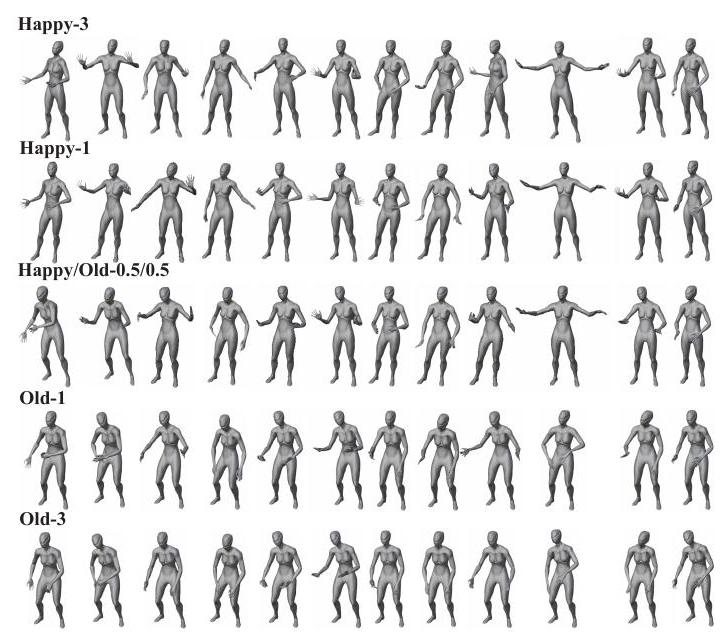
\includegraphics[width=0.6\linewidth]{images/style_sample.jpg}
%    \caption[Chỉnh sửa phong cách và nội suy]{\small Chỉnh sửa phong cách và nội suy. Từ trên xuống dưới, cơ thể xoắn và chuyển động tay dần giảm và vị trí tay trở nên thấp hơn. Mặc dù có sự thay đổi về phong cách, các cử chỉ được tạo ra vẫn khớp tốt với bài nói trong các phong cách khác nhau}
%    \label{fig:stylesample}
%\end{figure}


% % Hình 6: 



%Kết quả cho thấy rằng mô hình của luận văn tương tự như ExampleGesture về mặt phù hợp giữa phong cách cử chỉ của kết quả ở $\gamma=1$, và độ giống con người cũng như sự phù hợp với ngôn ngữ của luận văn vượt quá ExampleGesture. Trong khi đó, phong cách trở nên đáng kể hợp lý hơn khi $\gamma$ tăng, nhưng điểm của hai chiều khác giảm. Điều này cũng là hiển nhiên, tức là nếu cường độ của phong cách 'Old' quá cao, tay ít được nâng lên và toàn bộ chuỗi chuyển động có biên độ nhỏ, vì vậy nó trông ít giống con người hơn và ít phù hợp với ngôn ngữ nói. Chúng tôi cũng thấy rằng kết quả của việc tạo ra kiểm soát phong cách (\ref{fig:mosscore}) đã giảm so với kết quả của việc trực tiếp tạo ra phong cách tương ứng với ngôn ngữ nói (\ref{fig:mosscore}). Chúng tôi tin rằng việc kiểm soát một phong cách nói để tạo ra một phong cách của cử chỉ khác là một nhiệm vụ "khó khăn và xung đột" bởi vì phong cách nói và phong cách của cử chỉ vẫn liên quan và kết hợp với nhau.

% \subsection{Khả năng tạo ra các cử chỉ đa dạng}

% \begin{figure}
%     \centering
%     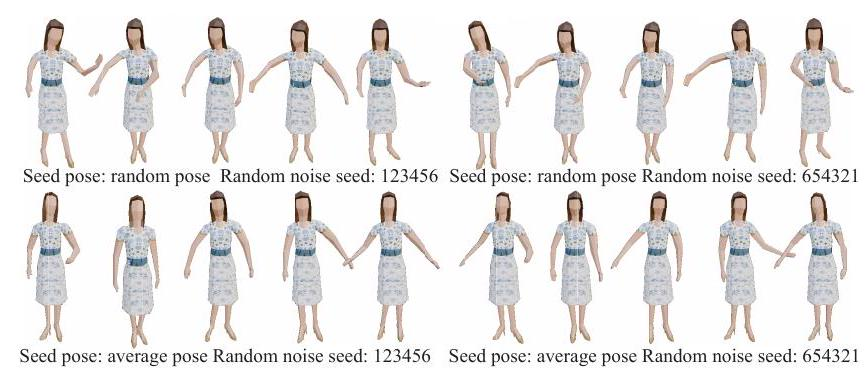
\includegraphics[width=\linewidth]{images/random_gesture_result.jpg}
%     \caption[Sự đa dạng của các cử chỉ]{Sự đa dạng của các cử chỉ. Mọi người thực hiện các cử chỉ đồng thoại khác nhau ở những thời điểm khác nhau trong các trạng thái khác nhau. Giống như con người thực tế, đối với cùng một bài nói, phương pháp của luận văn có khả năng tạo ra các cử chỉ khác nhau với hạt gieo khác nhau hoặc với cử chỉ nhiễu khác nhau}
%     \label{fig:randomgestureresult}
% \end{figure}


% \begin{center}
% \begin{tabular}{lcc}
% \hline
% \multicolumn{1}{c}{Tên} & \begin{tabular}{c}
% Con người $_{\text {tương đồng }} \uparrow$ \
% giống \
% \end{tabular} & \begin{tabular}{c}
% Phù hợp \
% ngôn ngữ - cử chỉ \
% \end{tabular} \
% \hline
% Sự thật & $4.15 \pm 0.11$ & $4.25 \pm 0.09$ \
% Chúng tôi & $\mathbf{4 . 1 1} \pm \mathbf{0 . 0 8}$ & $\mathbf{4 . 1 1} \pm \mathbf{0 . 1 0}$ \

% WavLM & $4.05 \pm 0.10$ & $3.91 \pm 0.11$ \
% tập trung chéo cục bộ & $3.76 \pm 0.09$ & $3.51 \pm 0.15$ \
% tập trung tự & $3.55 \pm 0.13$ & $3.08 \pm 0.10$ \
% chú ý + GRU & $3.10 \pm 0.11$ & $2.98 \pm 0.14$ \
% tập trung xuôi & $3.75 \pm 0.15$ & $3.23 \pm 0.24$ \
% \hline
% \end{tabular}
% \end{center}


% % Bảng 1: Kết quả nghiên cứu rút gọn. '-' chỉ ra các mô-đun không được sử dụng và ' + ' chỉ ra các mô-đun bổ sung. Chữ đậm chỉ ra số liệu tốt nhất.

% Do kiến trúc mô hình của luận văn, thậm chí đối với cùng một bài nói và phong cách, các cử chỉ nhiễu khác nhau và các hạt gieo khác nhau có thể tạo ra kết quả khác nhau, như thể hiện trong \autoref{fig:randomgestureresult}. Điều này giống như bài nói thực của con người, tạo ra các cử chỉ đồng thoại đa dạng liên quan đến vị trí ban đầu. Phân tích của luận văn trước đó được thực hiện trên chiều phong cách. Lưu ý rằng mô hình cũng thêm một mặt nạ ngẫu nhiên vào xử lý của hạt gieo, vì vậy nó cũng có thể nội suy và mở rộng các hạt gieo khác nhau để kiểm soát việc tạo ra cử chỉ với vị trí ban đầu khác nhau và đa dạng.

% \begin{table}[h]
% \caption{Đánh giá độ tương đồng và phù hợp ngôn ngữ-cử chỉ của các mô hình}
% \label{tab:evaluation}
% \begin{tabularx}{\textwidth}{l*{2}{>{\centering\arraybackslash}X}}
% \toprule
% \textbf{Tên} & \textbf{Con người (Tương đồng)} & \textbf{Phù hợp ngôn ngữ-cử chỉ} \\
% \midrule
% Sự thật & $4.15 \pm 0.11$ & $4.25 \pm 0.09$ \\
% Chúng tôi & $\mathbf{4.11 \pm 0.08}$ & $\mathbf{4.11 \pm 0.10}$ \\
% WavLM & $4.05 \pm 0.10$ & $3.91 \pm 0.11$ \\
% Tập trung chéo cục bộ & $3.76 \pm 0.09$ & $3.51 \pm 0.15$ \\
% Tập trung tự & $3.55 \pm 0.13$ & $3.08 \pm 0.10$ \\
% Chú ý + GRU & $3.10 \pm 0.11$ & $2.98 \pm 0.14$ \\
% Tập trung xuôi & $3.75 \pm 0.15$ & $3.23 \pm 0.24$ \\
% \bottomrule
% \end{tabularx}
% \end{table}

% \caption{Kết quả nghiên cứu rút gọn. '-' chỉ ra các mô-đun không được sử dụng và ' + ' chỉ ra các mô-đun bổ sung. Chữ đậm chỉ ra số liệu tốt nhất.}

% \section{Các thông tin thực nghiệm bổ sung}

% Hơn nữa, luận văn thực hiện nghiên cứu giảm thiểu để đánh giá ảnh hưởng hiệu suất của các thành phần khác nhau trong mô hình của luận văn. Vì phù hợp giữa cử chỉ và phong cách có thể được kiểm soát bằng tham số và ảnh hưởng đến hai chiều còn lại, luận văn đặt $\gamma$ là 1 và chỉ đánh giá sự giống nhân văn và phù hợp giọng nói để dễ so sánh. Kết quả của nghiên cứu giảm thiểu của luận văn được tóm tắt trong Bảng 1. Các so sánh hình ảnh của nghiên cứu này cũng có thể được tham khảo trong video bổ sung. Chúng tôi khám phá độ hiệu quả của các thành phần sau đây:
% (1) features WavLM 
% (2) local attention
% (3) local attention pattern
% (4) self-attention
% (5) attention
% Chúng tôi tiến hành thực nghiệm trên từng thành phần trong năm thành phần này, mỗi thành phần một lần.

% \subsection{Nghiên Cứu Người Dùng}
% Được hỗ trợ bởi kết quả trong Bảng 1, khi luận văn không sử dụng đặc trưng WavLM mà thay vào đó sử dụng 13 hệ số đầu tiên của hệ số cepstral tần số Mel (MFCC), điểm số của cả hai chiều đều giảm, đặc biệt là phù hợp giọng nói. Điều này là do các đặc trưng được trích xuất bởi mô hình WavLM đã được huấn luyện trước chứa nhiều thông tin như ngữ nghĩa và cảm xúc, giúp tạo ra các cử chỉ tương ứng. Khi không có sự chú ý cục bộ chéo, điểm số của cả hai chiều giảm rất nhiều. Bởi vì nhiều bước tạo ra cử chỉ chỉ liên quan đến các tương quan trong phạm vi ngắn, chú ý cục bộ có thể nắm bắt thông tin cục bộ tốt hơn, điều này khớp với quan sát của \cite{rae2020transformers}. Chỉ có chú ý tự dựa vào thông tin toàn cầu của các dãy dài trở nên ít hiệu quả hơn. 
% Cả giống nhân văn và sự phù hợp giữa cử chỉ và giọng nói giảm nhiều hơn khi chúng ta loại bỏ chú ý tự, ngụ ý rằng chú ý tự quan trọng hơn chú ý cục bộ vì có sự không đồng bộ tích cực giữa giọng nói và cử chỉ, và khó khăn để học đủ thông tin cử chỉ từ chỉ một cửa sổ cục bộ (gần như nửa giây) của giọng nói.
% Khi không sử dụng chú ý, luận văn thay thế nó bằng một mô hình dựa trên GRU, có kết quả tồi tệ nhất trong tất cả các mô hình, làm rõ thêm hiệu suất của cơ chế chú ý. 
% Ngoài ra, luận văn thực nghiệm sử dụng cấu trúc chú ý trong \autoref{fig:type_attention} và thấy rằng hiệu ứng trở nên tồi tệ hơn. Sự khác biệt duy nhất giữa việc thêm chú ý chuyển tiếp và chú ý cục bộ sử dụng trong mô hình của luận văn là cử chỉ được tạo ra với việc nhìn thêm vào thông tin giọng nói trong một cửa sổ tương lai. Điều này là một phát hiện thú vị, mặc dù có sự không đồng bộ ngầm giữa giọng nói và cử chỉ, theo một số cách, nó có thể chỉ ra rằng cử chỉ có liên quan hơn đến một khoảng thời gian ngắn trong hiện tại và quá khứ và không phải là một khoảng thời gian ngắn trong tương lai. Nó cũng có thể có khả năng rằng những người khác nhau có các phong cách khác nhau và tập dữ liệu này chỉ có một diễn viên cần được nghiên cứu thêm.

%\section{Kết quả minh hoạ sau quá trình render}
%
%\begin{quote}
%	{
%		"Your work is gonna fill a large part of your life . And the only way to be truly satisfied is to do what you believe is great work and the only way to do great work is to love what you do."}
%\end{quote}
%
%\begin{figure}[h]
%	\centering
%	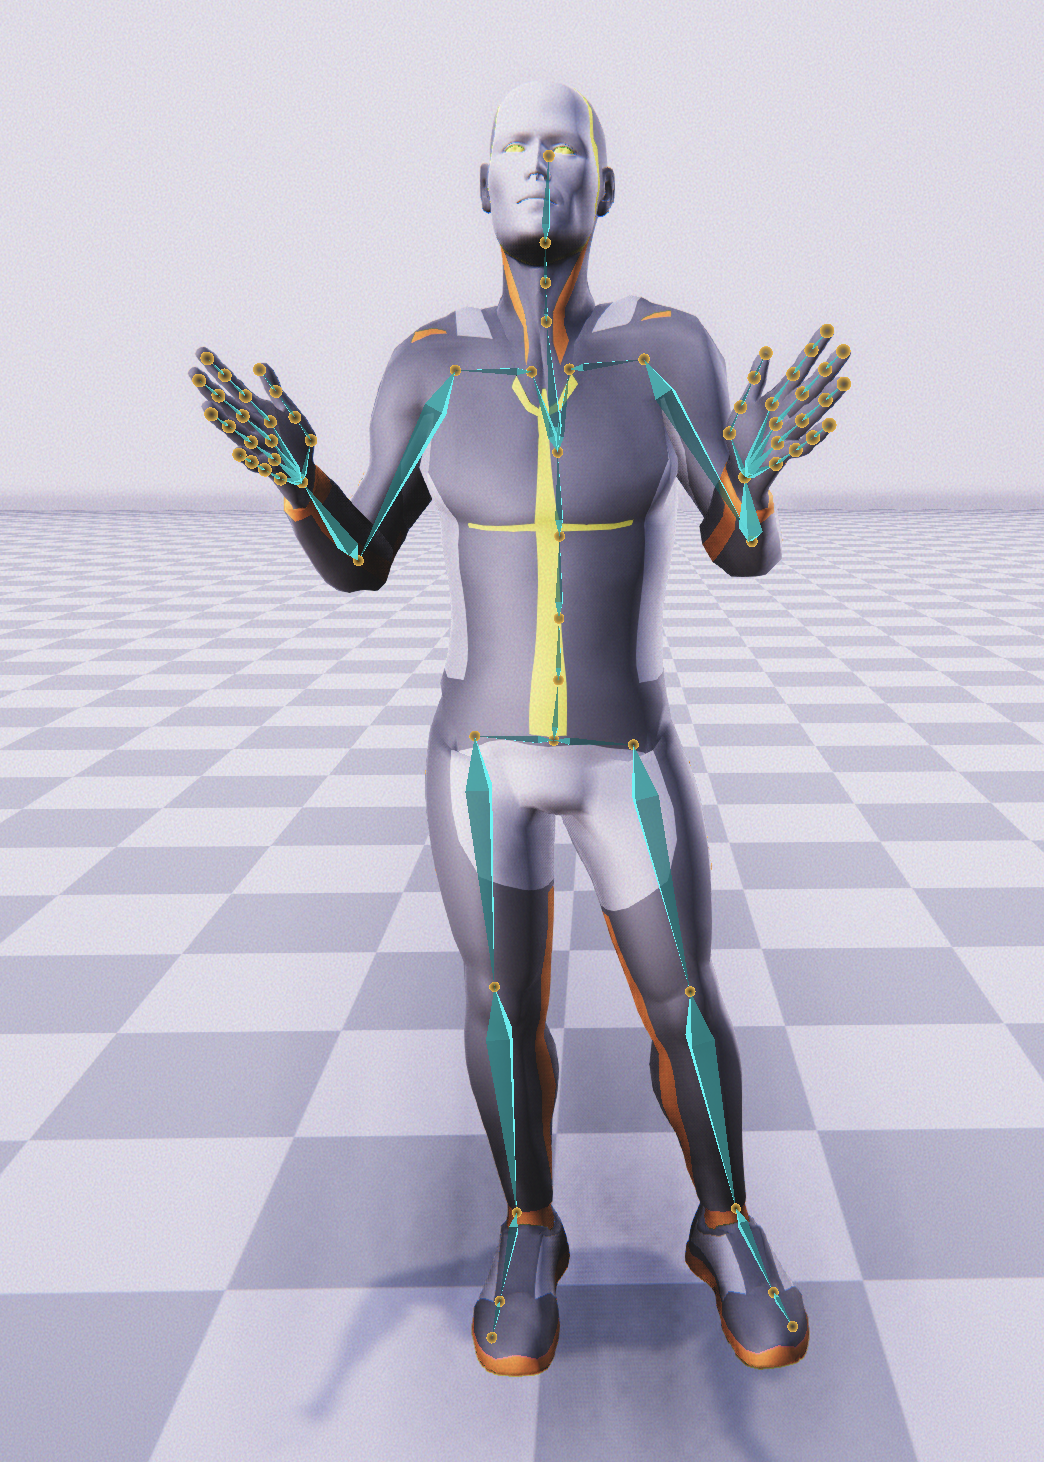
\includegraphics[height={6cm}]{SampleAnimation}
%	
%	\caption{Steven Job - Speech-Driven Gesture Generation}
%	\label{fig:SampleAnimation}
%
%\end{figure}
%
%\href{https://www.youtube.com/watch?v=B6nv1kQmi-Q}{\textcolor{blue}{\uline{youtube.com/watch?v=B6nv1kQmi-Q}}}



\chapter{KẾT LUẬN}
\label{Chapter5}

\section{Kết quả đạt được}

Luận văn đã phát triển và thử nghiệm thành công mô hình sinh cử chỉ OHGesture, một hệ thống có khả năng tạo ra cử chỉ rất tự nhiên, mang lại cảm giác giống người. Điểm nổi bật của mô hình là khả năng đồng bộ chính xác giữa cử chỉ và cảm xúc, nội dung của giọng nói đầu vào, đồng thời có khả năng suy luận vượt ra khỏi các dữ liệu được huấn luyện ban đầu. Điều này có nghĩa là mô hình dựa trên Diffusion không chỉ phụ thuộc vào các mẫu dữ liệu cử chỉ đã được học mà còn có thể có tính khái quát hóa cao, và có thể sinh cử chỉ cho các giọng nói và ngữ cảnh có xác suất dữ liệu thấp.

Một điểm đáng chú ý khác trong nghiên cứu này là việc mở rộng dữ liệu đầu vào. Luận văn không chỉ giới hạn ở cử chỉ, giọng nói và nhãn cảm xúc mà còn tích hợp thêm các công cụ chuyển đổi văn bản thành giọng nói để chuyển giọng nói thành văn bản. Nhờ có thêm một đặc trưng về văn bản, mô hình có thể bổ sung thêm đặc trưng về ngữ nghĩa của cử chỉ và giúp mô hình có thêm nguồn thông tin để đạt kết quả sinh tốt hơn, đồng thời giúp hệ thống hiểu rõ hơn ngữ cảnh và tạo ra cử chỉ phù hợp với từng nội dung cụ thể.

\section{Ưu và nhược điểm của mô hình}

Mô hình sinh cử chỉ OHGesture có nhiều ưu điểm đáng kể, góp phần quan trọng trong việc phát triển các hệ thống tương tác người-máy tự nhiên và linh hoạt hơn. Tuy nhiên, vẫn còn một số nhược điểm để cải thiện hiệu quả trong tương lai.

\vspace{10pt}

\textbf{Ưu điểm:}

\begin{itemize}
	\item Độ chân thực cao: Dựa vào kết quả sinh cử chỉ, có thể thấy mô hình OHGesture đã đạt được kết quả sinh cử chỉ có độ giống người cao. Các cử chỉ sinh ra phản ánh được sắc thái và nhịp điệu của giọng nói, giúp hệ thống có khả năng phản hồi đồng bộ với thông tin cảm xúc và nội dung của giọng nói.
	
	\item Khả năng tổng quát tốt: Nhờ mô hình khử nhiễu có thể phủ được các điểm dữ liệu có các xác suất thấp, mô hình có thể suy luận cử chỉ cho các tình huống và trạng thái cảm xúc chưa từng xuất hiện trong tập huấn luyện, cho thấy tiềm năng ứng dụng trong nhiều bối cảnh thực tế.
	
	\item Có khả năng kiểm soát được nhiều đặc trưng khác nhau: Mô hình diffusion có khả năng điều khiển được các cảm xúc khác nhau, có khả năng nội suy trạng thái giữa các cảm xúc khác nhau.
	\end{itemize}

\textbf{Nhược điểm:}

\begin{itemize}
	\item Mô hình hiện chưa có khả năng suy luận theo thời gian thực (real time) và cần nhiều bước để ra kết quả cuối cùng.
	
	\item Thông tin đặc trưng theo $D=1141$ được xử lý như một tấm ảnh, không thể hiện đúng đặc trưng chuyển động.
	
	\item Phụ thuộc vào dữ liệu đầu vào chất lượng cao: Mô hình yêu cầu dữ liệu giọng nói đầu vào có chất lượng tốt và rõ ràng để đảm bảo độ chính xác của cử chỉ sinh ra. Khi giọng nói đầu vào bị nhiễu hoặc chứa nhiều biến thể cảm xúc khó phân biệt, độ chính xác của cử chỉ sinh ra có thể giảm sút.
	
	
\end{itemize}


\section{Phương hướng phát triển và nghiên cứu trong tương lai}


Trong tương lai, có nhiều hướng phát triển tiềm năng để cải thiện và mở rộng mô hình sinh cử chỉ OHGesture, nhằm đáp ứng tốt hơn các yêu cầu thực tế và nâng cao tính ứng dụng của hệ thống. Một số hướng nghiên cứu và phát triển chính bao gồm:

\begin{itemize}
	\item Tối ưu hóa mô hình để có thể suy luận theo thời gian thực, hiện tại mô hình phải chia chuỗi giọng nói, và kết quả sinh phải được  import vào Unity mới có thể render. Trong tương lai, luận văn mong muốn có thể xây dựng các hệ thống với thời gian thực. để có thể tương tác và tăng tính ứng dụng của mô hình
	
	\item Tối ưu hóa quá trình sampling và giảm số bước lấy mẫu: Hiện tại, quá trình sinh cử chỉ đòi hỏi một số bước lấy mẫu (sampling steps) tương đối lớn, ảnh hưởng đến tốc độ và hiệu quả của hệ thống. Việc tối ưu hóa để giảm số bước sampling mà không làm suy giảm chất lượng cử chỉ sinh ra sẽ giúp mô hình đáp ứng nhanh hơn và phù hợp cho các ứng dụng thời gian thực.
	
	\item Tích hợp và thử nghiệm các kỹ thuật embedding mới: Sử dụng các phương pháp embedding mới, đa dạng hóa thông tin đầu vào có thể giúp mô hình hiểu và phản ánh tốt hơn ngữ cảnh và cảm xúc của giọng nói. Đây cũng là một hướng phát triển để nâng cao khả năng của hệ thống trong việc sinh cử chỉ phù hợp với ngữ nghĩa của các ngôn ngữ khác nhau.
	
	\item Mở rộng sang các ngôn ngữ mới: Hiện tại, mô hình chủ yếu hoạt động với các dữ liệu giọng nói tiếng Anh. Nghiên cứu mở rộng mô hình để sinh cử chỉ cho các ngôn ngữ và nền văn hóa khác nhau sẽ là một bước tiến quan trọng, giúp hệ thống trở nên đa dạng và ứng dụng rộng rãi hơn.
	
	\item Kết hợp với mô hình DeepPhase \cite{starke2022deepphase} để đạt hiệu quả sinh cử chỉ thời gian thực: Mục tiêu của luận văn là tích hợp OHGesture với mô hình DeepPhase để phát triển hệ thống có khả năng phản hồi cử chỉ trong thời gian thực, ứng dụng trong các tình huống giao tiếp tự nhiên như hội thoại người-máy và các hệ thống điều khiển bằng giọng nói. Với mục tiêu là học các đặc trưng về pha của các chuyển động để có thể trích xuất được các đặc trưng chuyển động, thay vì sử dụng đặc trưng như một tấm ảnh của mô hình.
	
	\item Cải thiện đánh giá khách quan bằng các độ đo tự động: Để giảm sự phụ thuộc vào các đánh giá chủ quan, cần phát triển và tích hợp các phương pháp đánh giá tự động đáng tin cậy, cho phép mô hình có thể tự đánh giá và điều chỉnh theo các chỉ số khách quan.
\end{itemize}

\section{Đóng góp của luận văn}
\label{sec:contribution}

Trong luận văn này, luận văn đã phát triển hệ thống sinh cử chỉ OHGesture, với các đóng góp quan trọng như sau:

\begin{itemize}
	\item Phát triển mô hình sinh cử chỉ dựa trên Diffusion: Hệ thống OHGesture được thiết kế để tạo ra các cử chỉ đồng bộ với giọng nói đầu vào và phản ánh đúng cảm xúc. Mô hình này còn có khả năng tổng quát hóa, cho phép sinh cử chỉ ngay cả với các mẫu giọng nói ngoài dữ liệu huấn luyện, mang lại độ chân thực cao.
	
	\item Công khai mã nguồn và mô hình trên các nền tảng mở: Để thúc đẩy ứng dụng và cải tiến từ cộng đồng, luận văn đã cung cấp mã nguồn trên GitHub, luận văn mở rộng mã nguồn, và được công khai ở \hyperlink{https://github.com/hmthanh/OHGesture}{Github/OHGesture} \footnote{Mã nguồn Github \url{https://github.com/hmthanh/OHGesture}} và một phiên bản pretrained trên Huggingface \hyperlink{https://huggingface.co/openhuman/openhuman}{huggingface.co/openhuman/openhuman} \footnote{HuggingFace \url{https://huggingface.co/openhuman/openhuman}}, giúp các nhà nghiên cứu khác dễ dàng tiếp cận, tái hiện và mở rộng hệ thống.
	
	\item Tích hợp thêm văn bản và giọng nói chuyển ngữ trong quá trình sinh cử chỉ: Với tập dữ liệu ZeroEGGS chỉ bao gồm giọng nói, cử chỉ và nhãn cảm xúc, luận văn sử dụng các API của Azure và Google để phiên âm (transcribe) các tệp giọng nói thành văn bản. Giúp mở rộng dữ liệu đầu vào của mô hình sinh cử chỉ thêm đặc trưng văn bản, giúp hệ thống có thêm ngữ cảnh để sinh ra các cử chỉ phù hợp hơn với nội dung cụ thể.
	
	\item Đóng góp vào việc xây dựng hệ thống đánh giá chuẩn hóa: Chúng tôi phát triển một hệ thống xếp hạng trực tuyến \hyperlink{https://genea-workshop.github.io/leaderboard/}{GENEA Leaderboard} \footnote{GENEA Leaderboard: \url{https://genea-workshop.github.io/leaderboard/}} \cite{nagy2024towards} cho các mô hình sinh cử chỉ. GENEA Leaderboard sẽ thu thập và xử lý các dữ liệu cử chỉ từ nhiều nguồn ngôn ngữ và tập dữ liệu khác nhau, tạo thành một tập dữ liệu chuẩn hóa duy nhất. Xây dựng một bản xếp hạng để so sánh nhiều mô hình khác nhau. Và sử dụng người để đánh giá các mô hình sinh, giúp đánh giá chính xác kết quả sinh của cử chỉ so với các độ đo trước đây, vốn không thể đo được sự phức tạp và đa dạng trong chuyển động của cử chỉ tương ứng với giọng nói. Điều này giúp tạo nên một nền tảng dữ liệu thống nhất, hỗ trợ việc đánh giá đồng nhất giữa các mô hình. Từ đó thúc đẩy tính thống nhất trong lĩnh vực sinh cử chỉ trong cộng đồng nghiên cứu.
	
	\item Xây dựng công cụ trực quan hóa bằng Unity: Các hệ thống trực quan hóa cử chỉ hiện nay đều dựa trên Blender, và không đạt kết quả hiển thị tốt khi sinh cử chỉ, bằng việc kế thừa mã nguồn từ mô hình DeepPhase \cite{starke2022deepphase} để xây dựng hệ thống kết xuất bằng Unity \hyperlink{https://github.com/DeepGesture/deepgesture-unity}{Github/DeepGesture-Unity}
	\footnote{Hệ thống render quá trình sinh cử chỉ bằng Unity \url{https://github.com/DeepGesture/deepgesture-unity}}.
	
	\item Xây dựng hệ thống đánh giá cử chỉ bằng FGD (Fréchet Gesture Distance): Dựa trên mã nguồn FGD \cite{yoon2020speech}, luận văn xây dựng GestureScore và huấn luyện một mô hình mới để đánh giá sự khác nhau về phân bố dữ liệu về góc quay giữa dữ liệu dự đoán và dữ liệu thật. Mã nguồn của  \hyperlink{https://github.com/GestureScore/GestureScore}{GestureScore} \footnote{Github/GestureScore: \url{https://github.com/GestureScore/GestureScore}} và mô hình pretrain của mô hình đánh giá được công khai ở  \hyperlink{https://huggingface.co/GestureScore}{Huggingface} \footnote{Huggingface/GestureScore: \url{https://huggingface.co/GestureScore/GestureScore}}
	\item Xây dựng hướng phát triển trong tương lai: Dựa trên nền tảng của mô hình diffusion và hiểu rõ bản chất của quá trình sinh cử chỉ, luận văn có thể kết hợp các mô hình sinh cử chỉ dựa trên pha với các thuật toán xử lý và trích xuất thông tin, nhằm tối ưu hóa chất lượng và tính phù hợp của các cử chỉ được sinh ra. Hướng phát triển này mở ra triển vọng cho các cải tiến sâu rộng trong việc tương tác giữa cử chỉ và các yếu tố ngữ cảnh phức tạp như biểu cảm khuôn mặt, ngữ điệu và động lực cảm xúc, tạo nền tảng cho những bước tiến trong các ứng dụng giao tiếp người - máy và các lĩnh vực liên quan khác.
\end{itemize}



\newpage

\section{Lời kết}

Qua quá trình thử nghiệm và phân tích kết quả sinh cử chỉ thực tế, mô hình OHGesture của luận văn đã kế thừa và phát triển từ mô hình DiffuseStyleGesture, có khả năng sinh cử chỉ chân thực, không chỉ trên các mẫu dữ liệu trong tập huấn luyện mà còn mở rộng được với những giọng nói không có trong dữ liệu huấn luyện, ví dụ như giọng nói của Steve Jobs. Điều này minh chứng cho tiềm năng của mô hình Diffusion trong việc sinh cử chỉ cho các dữ liệu hiếm, nơi xác suất dữ liệu thấp.

Bên cạnh đó, luận văn đã đóng góp các mã nguồn chỉnh sửa trên Github, bao gồm quá trình kết xuất (render) và xử lý dữ liệu trên nền tảng Unity, tạo nền tảng thuận lợi cho các nghiên cứu và cải tiến tiếp theo đối với mô hình OHGesture. Việc kết hợp thêm văn bản vào quá trình sinh cử chỉ cũng là một bước đột phá, mở ra nhiều hướng phát triển ứng dụng trong các lĩnh vực yêu cầu tương tác tự nhiên và hiệu quả hơn.


\pagebreak 
%TÀI LIỆU TRÍCH DẪN
\renewcommand{\bibname}{TÀI LIỆU THAM KHẢO} % Đổi tên phần tiêu đề của tài liệu tham khảo
%
\bibliographystyle{plain}
%\bibliographystyle{custombibstyle}
\bibliography{References/references}



%\renewcommand{\bibname}{DANH MỤC CÔNG TRÌNH CỦA HVCH}
%\bibliographystyle{plain}
%\bibliography{References/author}
%\printbibliography[heading=subbibliography,
%title={Web Related},
%keyword=web]
%\chapter*{TRÍCH NGANG THÔNG TIN BÀI BÁO KHOA HỌC LIÊN QUAN ĐẾN LUẬN VĂN THẠC SĨ	}
%\label{AppendixAuthor}
\chapter*{DANH MỤC CÔNG TRÌNH CỦA HVCH}
\label{AppendixAuthor}

\begin{enumerate}
	\item Towards a GENEA Leaderboard -- an Extended, Living Benchmark for Evaluating and Advancing Conversational Motion Synthesis \cite{nagy2024towards}.
%\item Tạp chí XYZ
\end{enumerate}

%\printbibliography[heading=subbibliography, title={Tiếng Việt}, keyword=Viet, resetnumbers=true]
%\bibliography{References/author.bib}

%\printbibliography[heading=subbibliography,
%title={Web Related},
%keyword=thanhminh]

\appendix
\renewcommand{\chaptername}{Phụ lục}
\chapter{Các tham số trong Diffusion}
 \label{Appendix1}

\section{Sự thay đổi của $\sqrt{\alpha}$ và $\sqrt{1 - \alpha}$}

\setcounter{figure}{13}
\begin{figure}[H]
	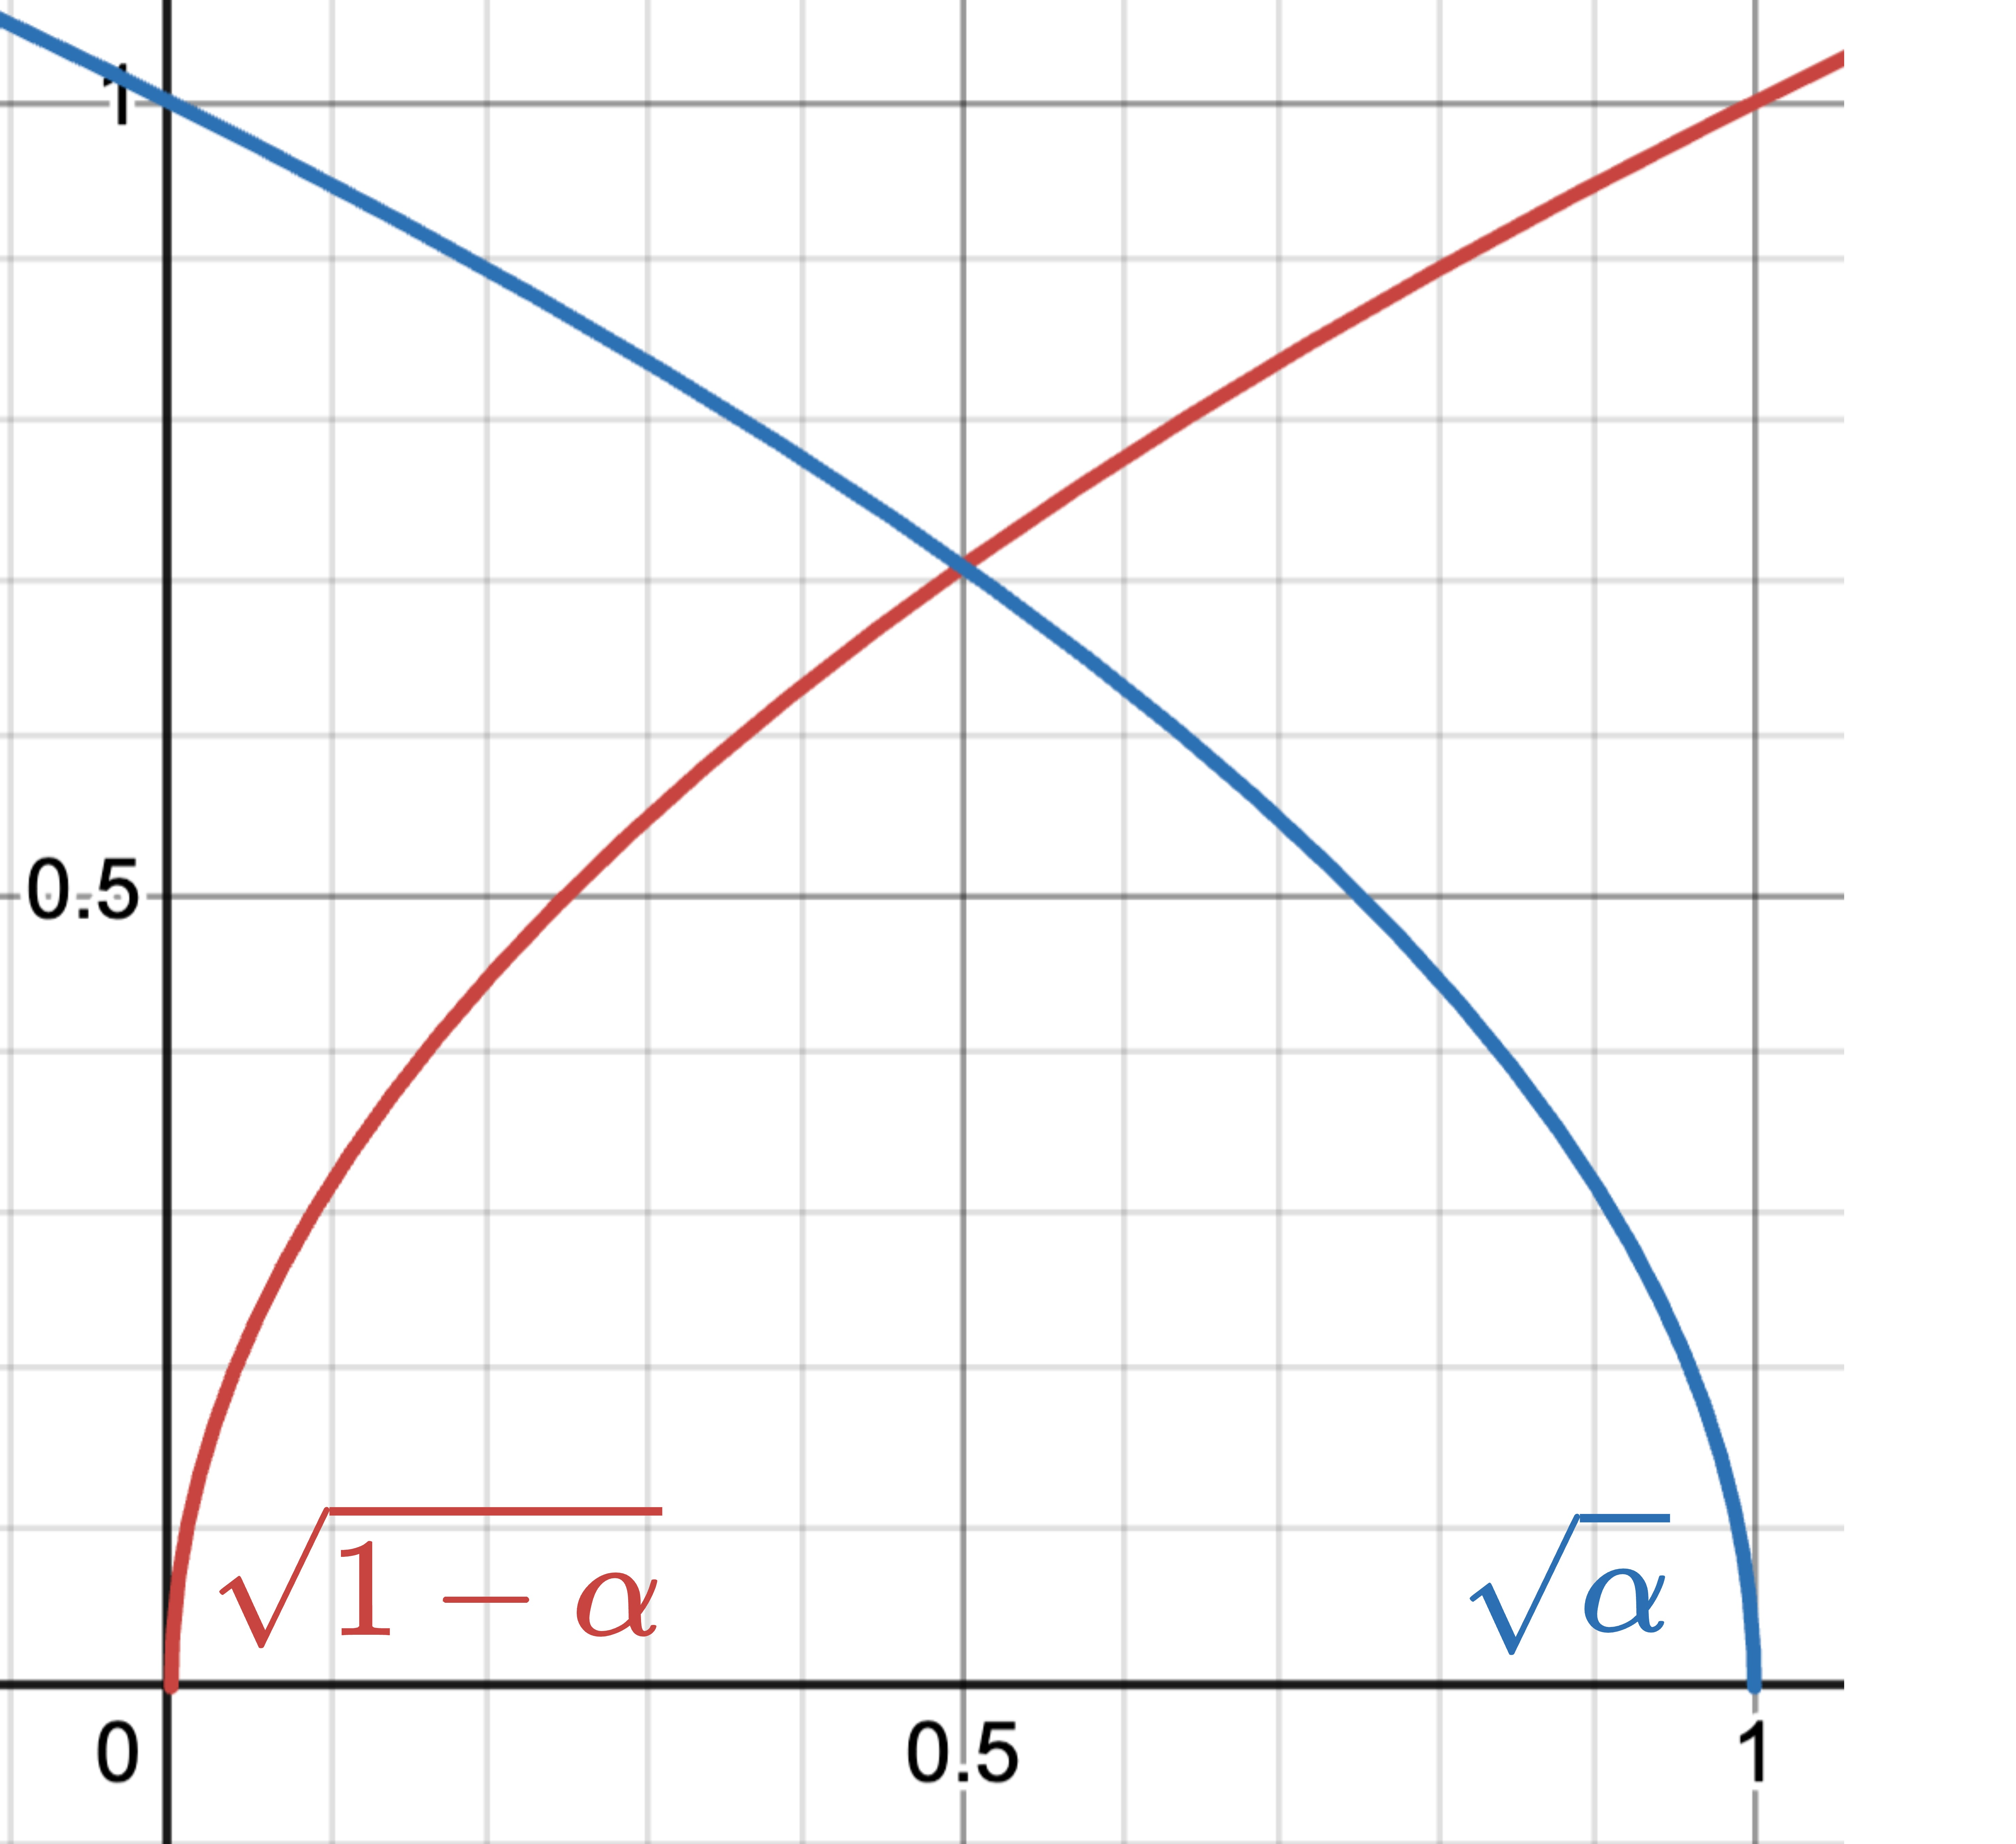
\includegraphics[width=0.5\linewidth]{SquareAlpha}
	\label{fig:wrapfig}
	\caption{Sự thay đổi của $\sqrt{\alpha}$ và $\sqrt{1 - \alpha}$}
\end{figure}

Trong quá trình diffusion, hệ thống muốn giảm dần sự hiện diện của $\bx$ và tăng dần sự hiện diện của nhiễu $\epsilon_t$. Với $\mathbf{x}_t = \sqrt{\alpha_t} \mathbf{x}_t + \sqrt{1 - \alpha_t} \epsilon_t$. Các hệ số $\sqrt{\alpha_t}$ và $\sqrt{1 - \alpha_t}$ giúp điều khiển quá trình này như sau:



\begin{itemize}
	\item $\sqrt{\alpha_t}$: Ban đầu giá trị lớn nhưng giảm dần để giảm sự ảnh hưởng vào kết quả tổng giữa nhiễu và $\bx_t$
	\item $\sqrt{1 - \alpha_t}$: Ban đầu giá trị nhỏ nhưng tăng dần theo từng bước. Với mục tiêu là đến cuối cùng thì sự ảnh hưởng của nhiễu càng lớn và trở thành nhiễu hoàn toàn.
\end{itemize}


Cả hai đại lượng này thay đổi theo thời gian trong quá trình diffusion, từ đó quyết định mức độ nhiễu được thêm vào từng bước $t$ và mức độ giữ lại trạng thái trước đó qua từng bước.


\section{Sự thay đổi của $\sqrt{\bar{\alpha}}$ và $\sqrt{1 - \bar{\alpha}}$}

$\bar{\alpha}_t = \prod_{i=1}^t \alpha_i$.  $\sqrt{1 - \bar{\alpha}_t} = \sqrt{1 - \prod_{i=1}^t \alpha_i}$. Cả $\sqrt{\bar{\alpha}}$ và $\sqrt{1 - \bar{\alpha}}$ đóng một vai trò quan trọng trong quá trình huấn luyện và sinh cử chỉ. Giúp kiểm soát mức độ nhiễu được thêm vào và cử chỉ, ta có thể thấy $\sqrt{\bar{\alpha}}$ giảm dần còn $\sqrt{1 - \bar{\alpha}}$ thì tăng dần..


\begin{figure}[H]
	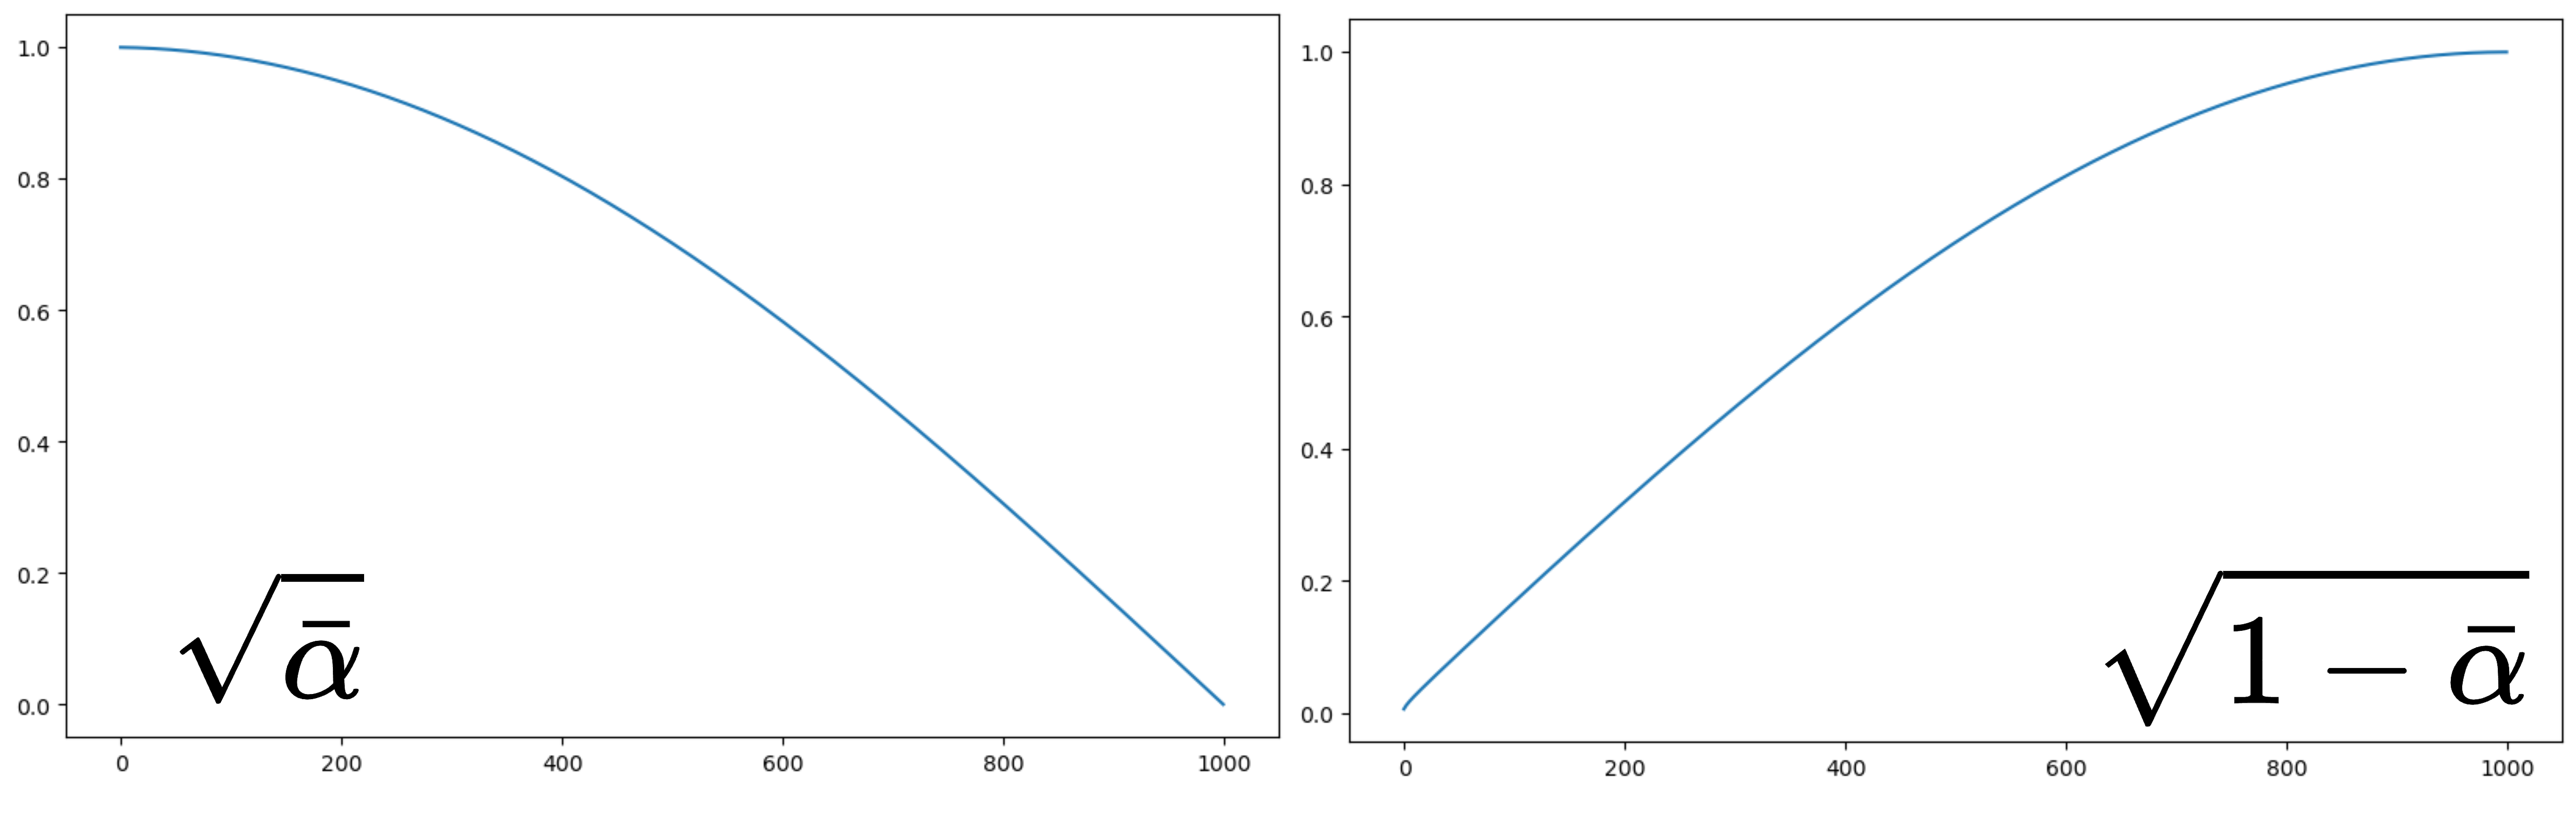
\includegraphics[width=\linewidth]{AlphaCumprod}
	\label{fig:AlphaCumprod}
	\caption{Quá trình thay đổi của $\sqrt{\bar{\alpha}}$ và $\sqrt{1 - \bar{\alpha}}$}
\end{figure}

\section{So sánh $\epsilon$ objective và  $\bx_0$ }

\begin{figure}[H]
	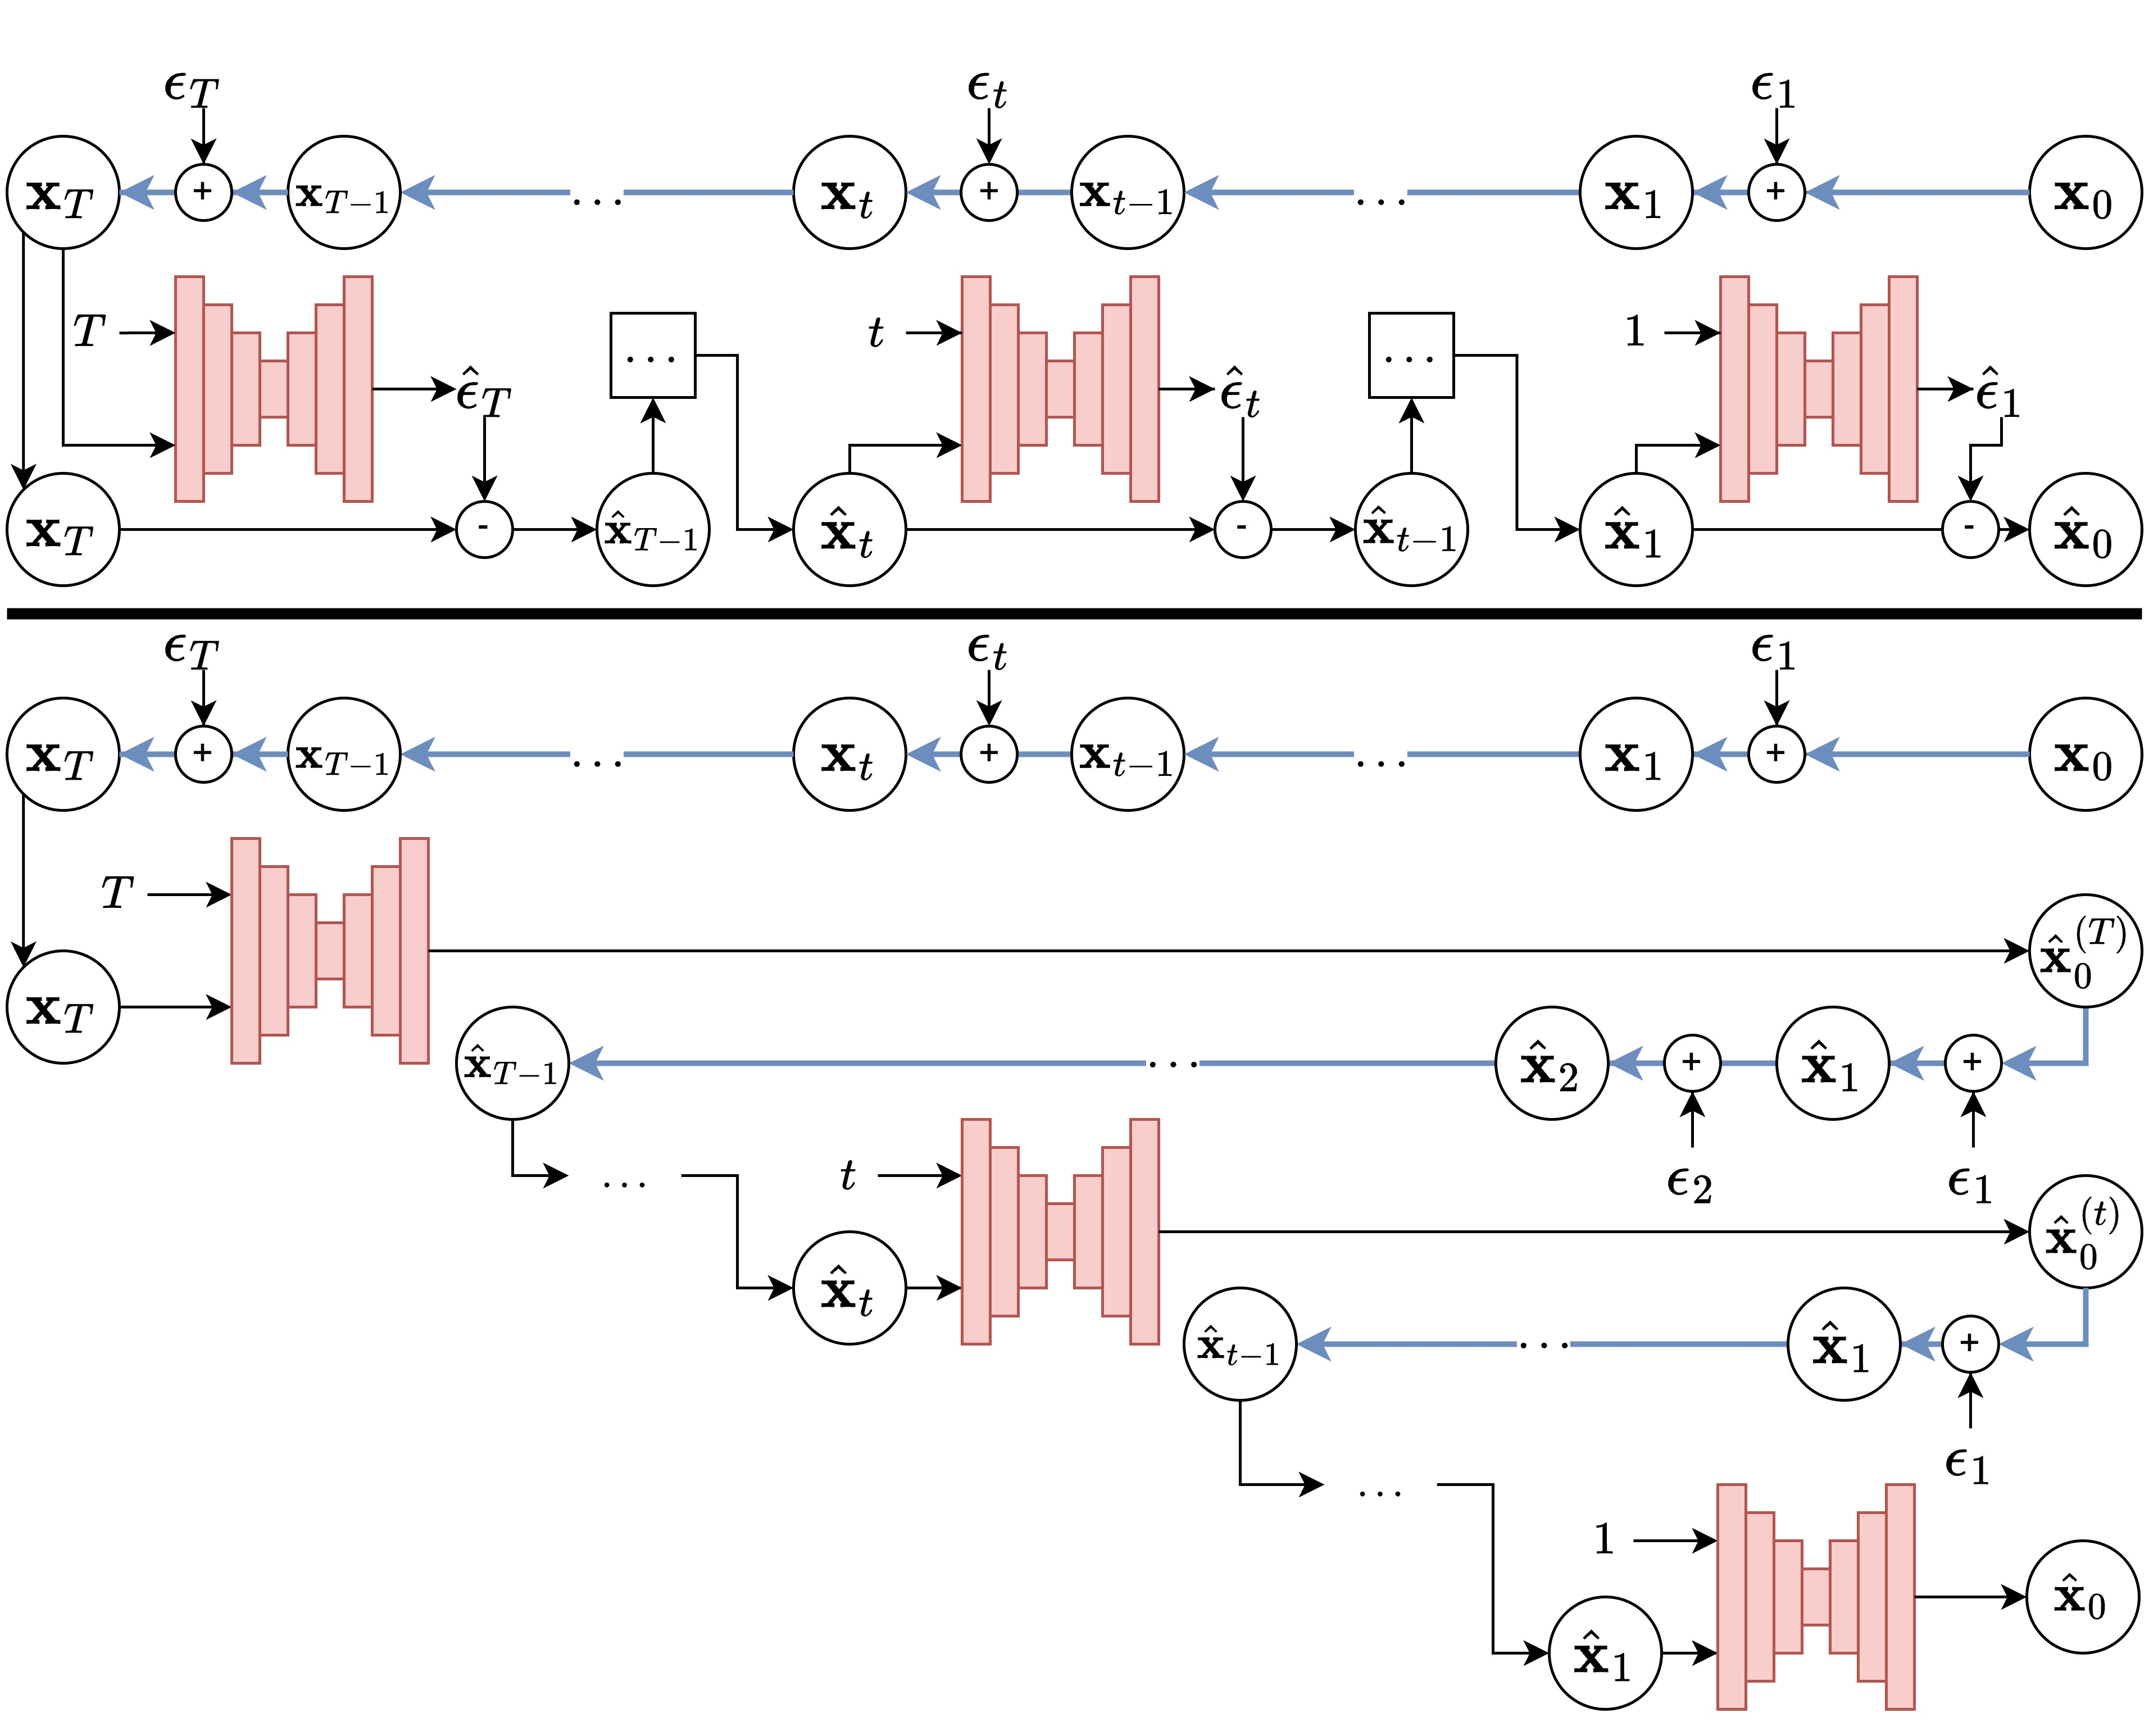
\includegraphics[width=\linewidth]{X0Objective}
	\label{fig:X0Objective}
	\caption{\textbf{So sánh $\epsilon$ objective (bên trên) và  $\bx_0$ (bên dưới)}. }
\end{figure}

\begin{itemize}
	\item \textbf{$\epsilon$  objective} :  mô hình sẽ dự đoán lỗi. Bắt đầu từ việc forward quá trình gây nhiễu để lấy được $\bx_T$, khi có được $\bx_T$ ta sẽ sử dụng $\bx_T \in \mathcal{N}(0, \mathbf{I})$ để đưa vào quá trình denoise. Trong quá trình denoise, mô hình sẽ dự đoán nhiễu $\hat{\epsilon}_t$ đã được thêm vào từ quá trình forward, là nhiễu $\epsilon_t$ và tối ưu lỗi giữa nhiễu dự đoán và nhiễu thực tế từ quá trình forward.
	\item \textbf{$\bx_0$ objective} : tương tự mô hình sẽ forward quá trình gây nhiễu để lấy được $\bx_T$, khi có được $\bx_T$ ta sẽ sử dụng $\bx_T \in \mathcal{N}(0, \mathbf{I})$ để đưa vào quá trình denoise. Mô hình sẽ dự đoán trực tiếp $\bx_0$, sau khi có $\bx_0$ mô hình sẽ tiếp tục gây nhiễu (Diffuse ) đến bước thứ $\bx_{t-1}$, và tiếp tục sử dụng $\bx_{t-1}$ để đưa vào mô hình dự đoán $\bx_0$
	\end{itemize}



%Praesent in sapien. Lorem ipsum dolor sit amet, consectetuer 
%adipiscing elit. Duis fringilla tristique neque. Sed interdum

%\begin{figure*}[p]
%	\centering
%	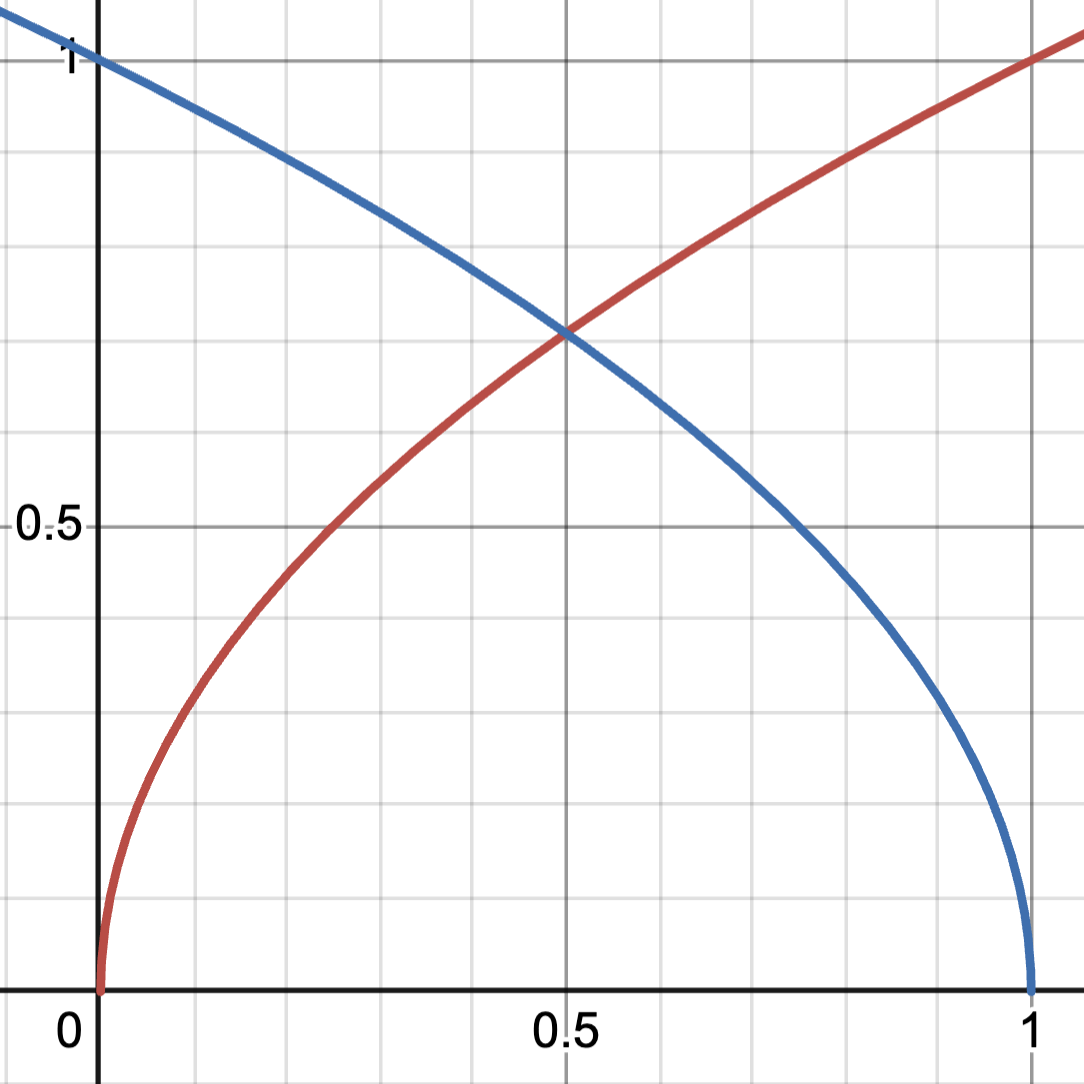
\includegraphics[width=0.5\linewidth]{images/beta_sqrtbeta}
%	\caption{Sự thay đổi của $\sqrt{\beta}$ và $\sqrt{1-\beta}$}
%	\label{fig:beta_sqrtbeta}
%\end{figure*}


%You can put more than one value in the parameter, for instance, if you write [ht] LaTeX will try to position the figure here, but if it's not possible (the space may be insufficient) then the figure will appear at the top of the page. It is recommended to use more than one positioning parameter to prevent unexpected results.

\chapter{Quá trình xử lý dữ liệu BVH}
\label{Appendix2}

\section{Cấu trúc khung xương của một nhân vật}

Một số tên khung xương nhân vật trong $75$ khung xương chuyển động bao gồm:

{
\small
\texttt{Hips},
\texttt{Spine},
\texttt{Neck},
\texttt{Head},
\texttt{RightShoulder},
\texttt{RightArm},
\texttt{RightForeArm},
\texttt{RightHand},
\texttt{LeftShoulder},
\texttt{LeftArm},
\texttt{LeftForeArm},
\texttt{LeftHand},
\texttt{RightUpLeg},
\texttt{RightLeg},
\texttt{RightFoot},
\texttt{RightToeBase},
\texttt{LeftUpLeg},
\texttt{LeftLeg},
\texttt{LeftFoot},
\texttt{LeftToeBase},
...
}

%\begin{itemize}
%	\item Left
%\end{itemize}

%\begincolcol}

\begin{figure}[H]
\centering
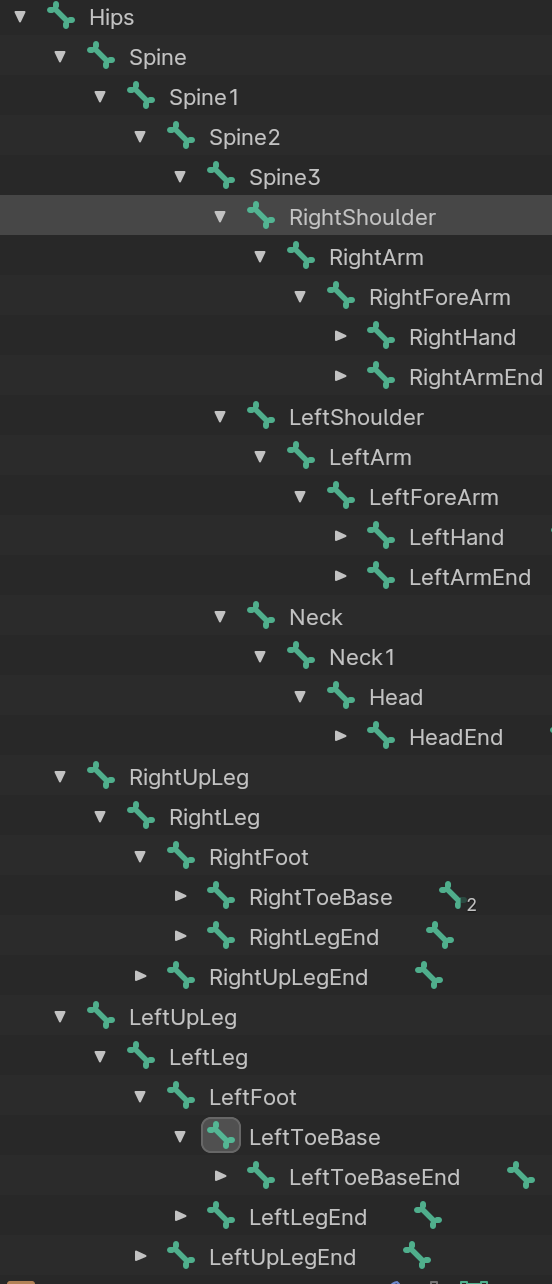
\includegraphics[height=10.5cm]{Bone}
\caption{Khung xương của một nhân vật}
\label{fig:Bone}
\end{figure}

\section{Cấu trúc tệp dữ liệu BVH}


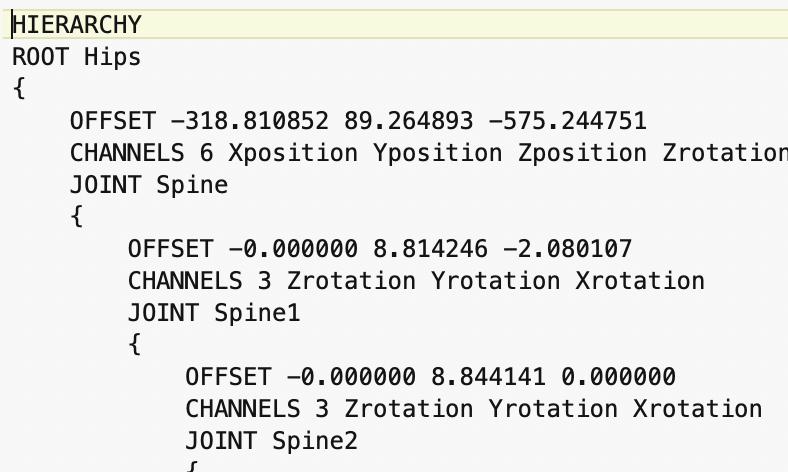
\includegraphics[width=0.4\linewidth]{BVHFile}
File BVH (Biovision Hierarchy) là một định dạng file dữ liệu chứa thông tin về cấu trúc xương và dữ liệu về chuyển động của xương trong một hệ thống xương. File BVH bao gồm hai phần chính: phần khai báo cấu trúc xương và phần dữ liệu chuyển động của xương. 
%Mỗi phần được phân cách bởi từ khóa \texttt{MOTION}.

\setcounter{figure}{15}
\begin{figure}
	\centering
	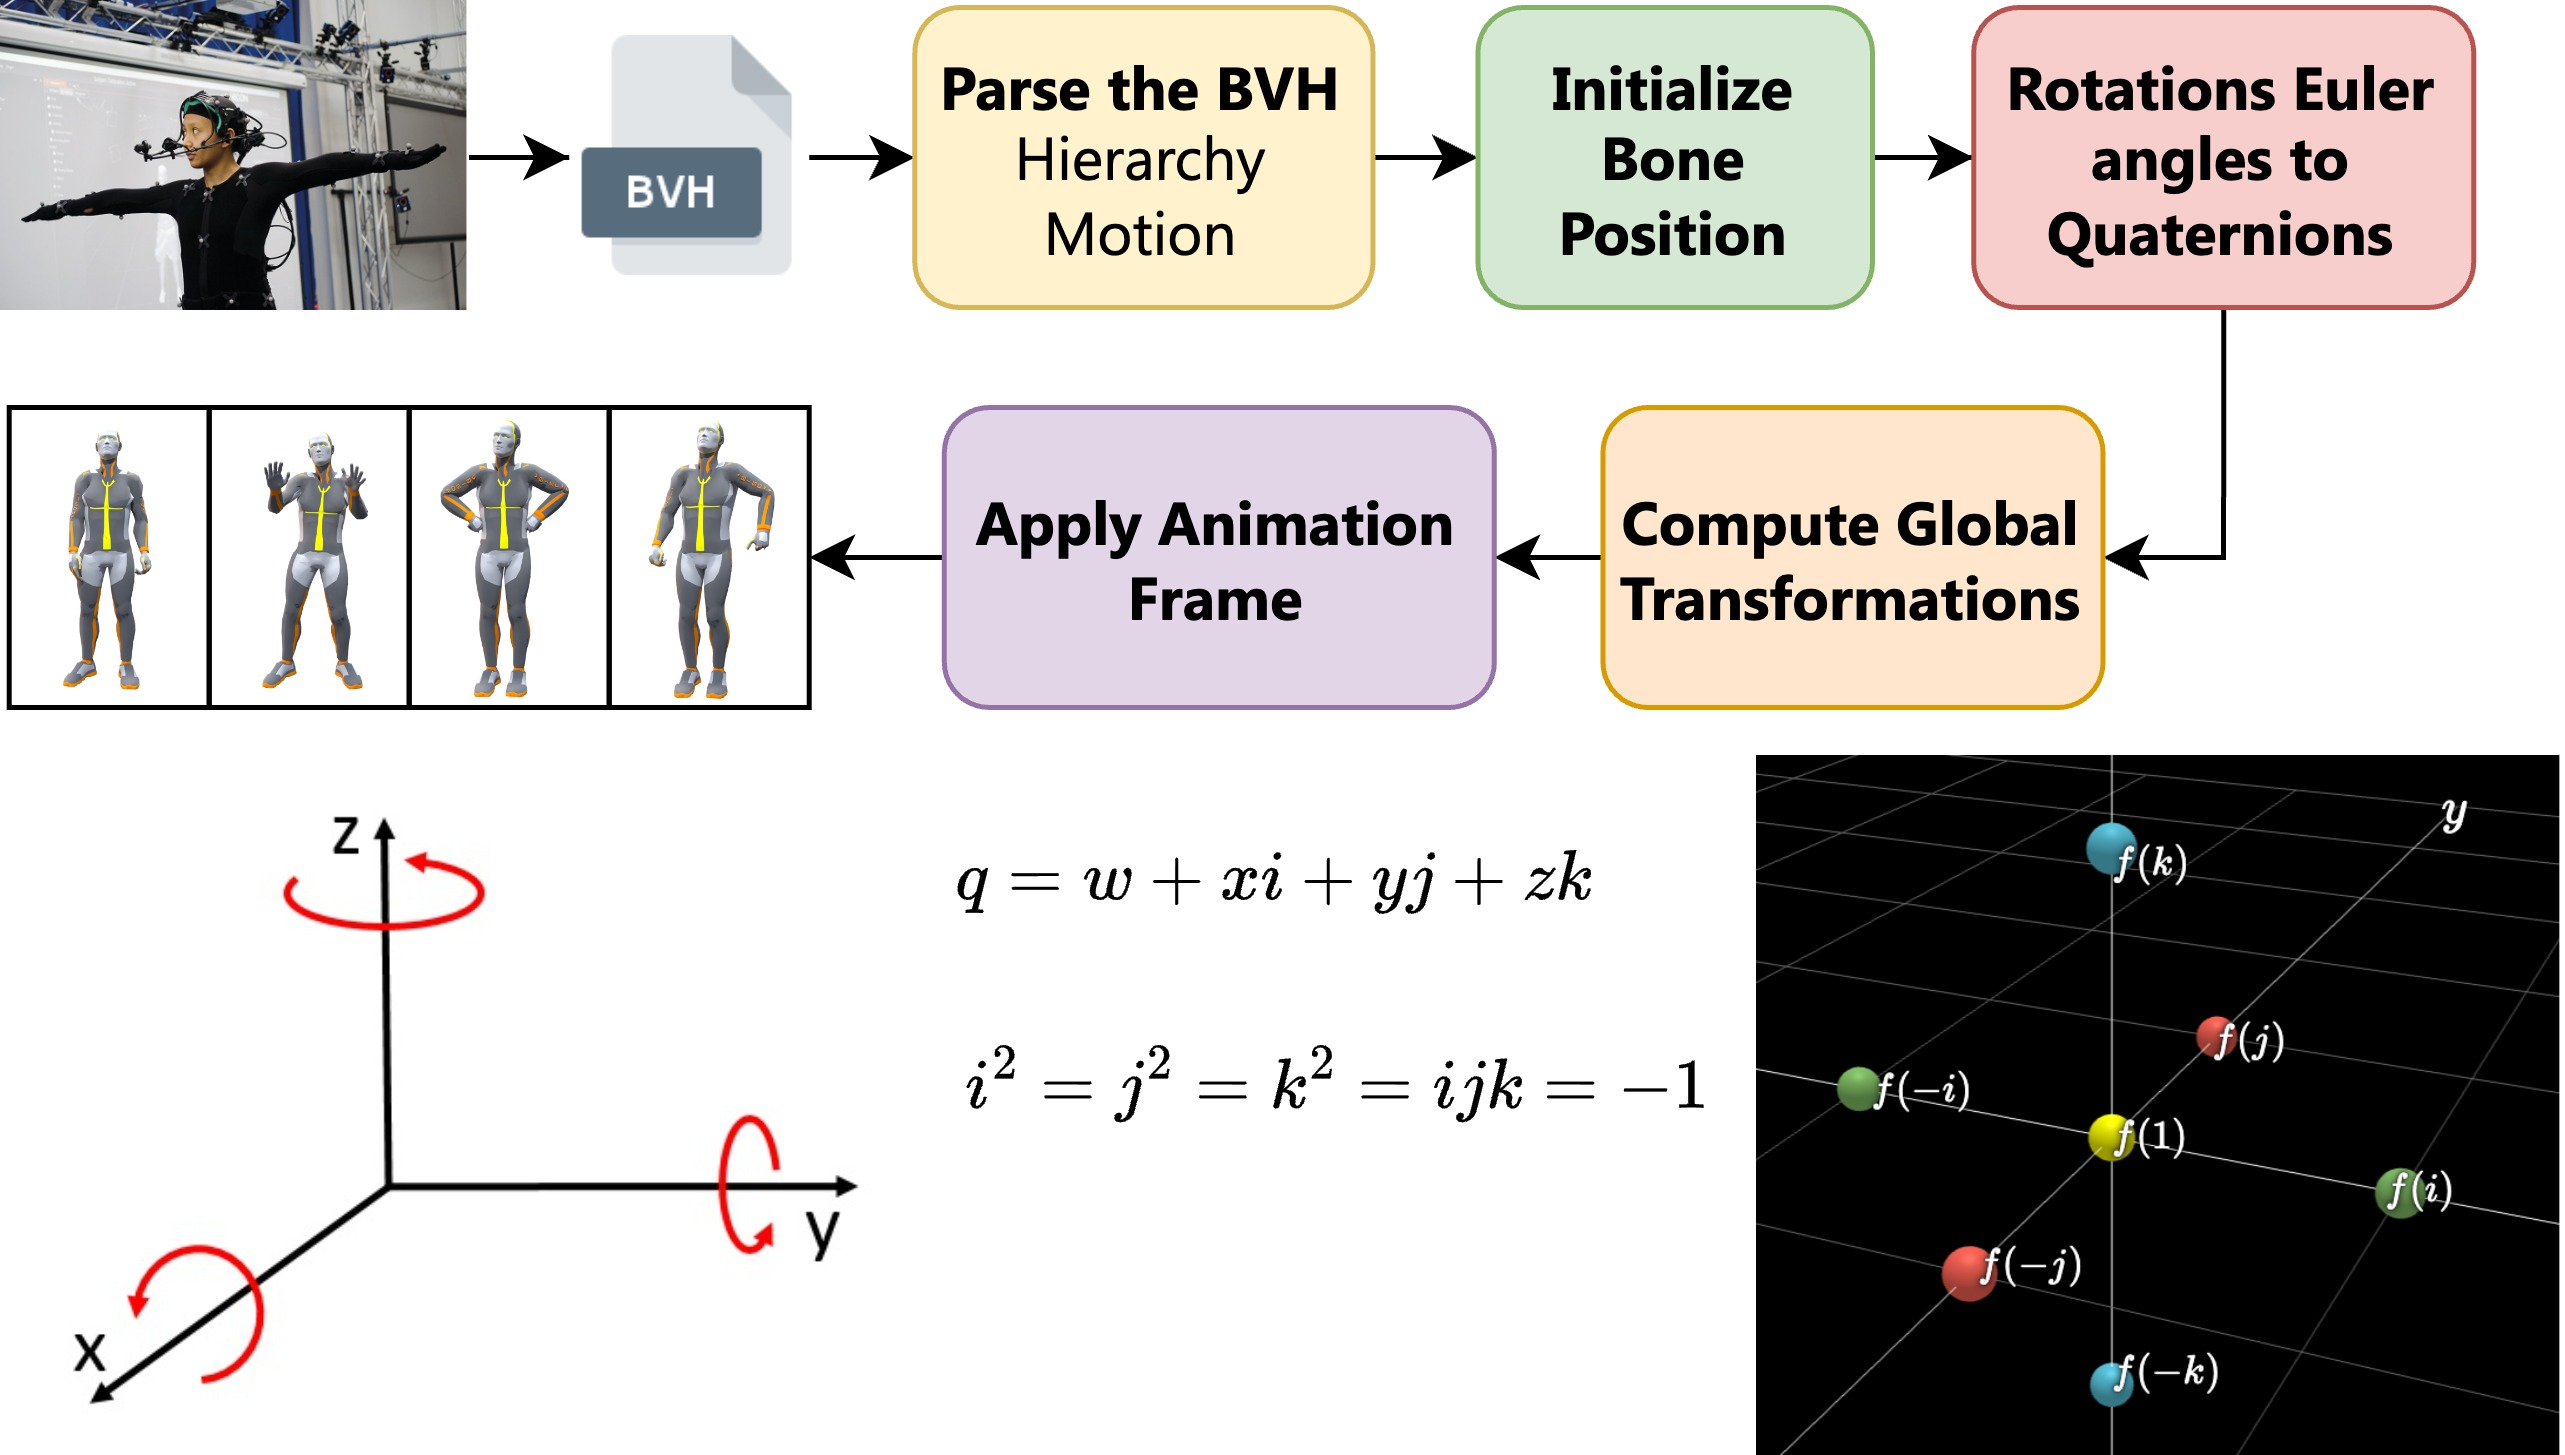
\includegraphics[width=\linewidth]{BVH}
	\caption{Quá trình xử lý tệp tin BVH}
	\label{fig:BVH}
\end{figure}


%	\begin{figure}
	%		\centering
	%		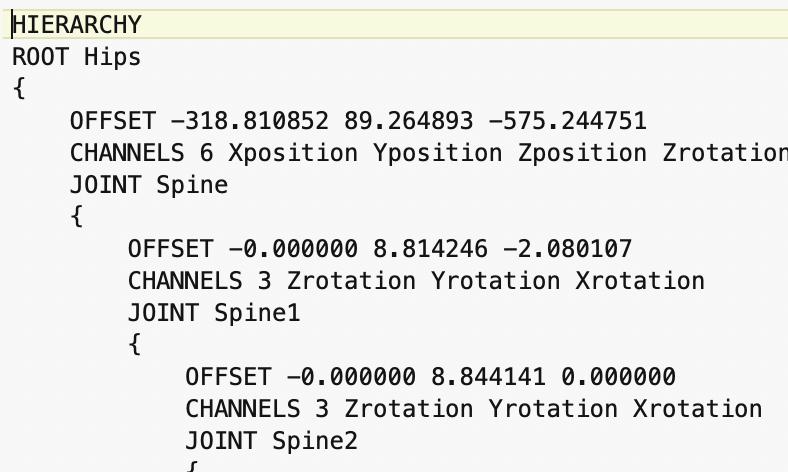
\includegraphics[width=0.25\textwidth]{BVHFile}
	%	\end{figure}
	
$\mathbf{rotation}_i^{\operatorname{local}} = \{ \alpha ,\beta , \gamma \}$ lần lượt là góc quay quanh các trục $Z$ ,$Y$ , và $X$, góc quay tổng hợp ba trục trong không gian Eule là 

\begin{equation}
R = R_Z(\alpha) R_Y(\beta) R_X(\gamma)
\end{equation}

Trong đó:

1. \textbf{Ma trận quay quanh trục \(Z\)}:

\[
R_Z(\alpha) = 
\begin{bmatrix}
	\cos(\alpha) & -\sin(\alpha) & 0 \\
	\sin(\alpha) & \cos(\alpha) & 0 \\
	0 & 0 & 1
\end{bmatrix}
\]

2. \textbf{Ma trận quay quanh trục \(Y\)}:

\[
R_Y(\beta) = 
\begin{bmatrix}
	\cos(\beta) & 0 & \sin(\beta) \\
	0 & 1 & 0 \\
	-\sin(\beta) & 0 & \cos(\beta)
\end{bmatrix}
\]

3. \textbf{Ma trận quay quanh trục \(X\)}:

\[
R_X(\gamma) = 
\begin{bmatrix}
	1 & 0 & 0 \\
	0 & \cos(\gamma) & -\sin(\gamma) \\
	0 & \sin(\gamma) & \cos(\gamma)
\end{bmatrix}
\]

Để tính toạ độ chuyển động của một nhân vật, ta thực hiện phép toán sau:

\begin{equation}
	\mathbf{position}_{\text{global}} = R \cdot \mathbf{position}_{\text{local}} + \mathbf{t}
\end{equation}


\section{Quá trình chuyển góc quay Euler sang Quaternion}

%Quaternion là một cách biểu diễn góc quay trong không gian ba chiều. Quaternion có dạng $q = a + bi + cj + dk$, trong đó $ư, b, c, d$ là các số thực. Quaternion có thể được biểu diễn dưới dạng ma trận $4 \times 4$ như sau:


Để tránh Gimbal lock, ta phải chuyển dữ liệu ở dạng góc quay Euler sang dạng góc quay Quaternion. Trong đó góc quay từng Bone dạng Euler ZYX sang dạng Quaternion, mỗi Bone biểu diễn bằng 4 phần tử $q = (q_w, q_x, q_y, q_z)$, với các giá trị được tính như sau:
%	Mỗi Bone được biểu diễn thành: 
%	$$q = w + xi + yj + zk$$
%	c
%	$$i^2 = j^2 = k^2 = ijk = -1$$

Đầu tiên, chúng ta tính các giá trị $\cos$ và $\sin$ của một nửa góc quay cho mỗi trục:


\begin{itemize}
	\item $c_{\alpha} = \cos\left(\frac{\alpha}{2}\right), \quad s_{\alpha} = \sin\left(\frac{\alpha}{2}\right)$
	\item $c_{\beta} = \cos\left(\frac{\beta}{2}\right), \quad s_{\beta} = \sin\left(\frac{\beta}{2}\right)$
	\item $c_{\gamma} = \cos\left(\frac{\gamma}{2}\right), \quad s_{\gamma} = \sin\left(\frac{\gamma}{2}\right)$
\end{itemize}

Dựa trên các giá trị tính được ở trên, các thành phần của quaternion được tính như sau:


\begin{itemize}
	\item $q_w = c_{\alpha} c_{\beta} c_{\gamma} + s_{\alpha} s_{\beta} s_{\gamma}$
	\item $q_x = c_{\alpha} c_{\beta} s_{\gamma} - s_{\alpha} s_{\beta} c_{\gamma}$
	\item $q_y = c_{\alpha} s_{\beta} c_{\gamma} + s_{\alpha} c_{\beta} s_{\gamma}$
	\item $q_z = s_{\alpha} c_{\beta} c_{\gamma} - c_{\alpha} s_{\beta} s_{\gamma}$
\end{itemize}

Với quaternion $q$ đã tính, vị trí toàn cục của bone $\mathbf{p}_{\text{global}}$ được xác định bằng cách quay vị trí cục bộ $\mathbf{p}_{\text{local}}$ thông qua công thức:

\begin{equation}
	\mathbf{p}_{\text{global}} = q \cdot \mathbf{p}_{\text{local}} \cdot q^{-1} + \mathbf{t}
\end{equation}

với $\mathbf{t}$ là vị trí gốc của bone trong không gian toàn cục.




\chapter{Training và Sampling}
\label{Appendix3}

\section{Thuật toán Training trong Diffusion cơ bản}
\begin{algorithm}[H]
	\caption{Training} \label{alg:training}
	\begin{algorithmic}[1]
		\footnotesize
		\Repeat
		\State $\bx_0 \sim q(\bx_0)$
		\State $t \sim \mathrm{Uniform}(\{1, \dotsc, T\})$
		\State $\bepsilon\sim\mathcal{N}(\bzero,\bI)$
		\State Take gradient descent step on
		\Statex $\qquad \grad_\theta \left\| \bepsilon - \bepsilon_\theta(\mathbf{x}_t, t) \right\|^2$
		\Until{converged}
	\end{algorithmic}
\end{algorithm}

\section{Thuật toán Sampling trong Diffusion cơ bản}

\begin{algorithm}[H]
	\caption{Sampling} \label{alg:sampling}
	\footnotesize
	\begin{algorithmic}[1]
		\footnotesize
		\State $\bx_T \sim \mathcal{N}(\bzero, \bI)$
		\For{$t=T, \dotsc, 1$}
		\State $\bz \sim \mathcal{N}(\bzero, \bI)$ if $t > 1$, else $\bz = \bzero$
		\State $\mu = \frac{1}{\sqrt{\alpha_t}}\left( \bx_t - \frac{1-\alpha_t}{\sqrt{1-\bar\alpha_t}} \bepsilon_\theta(\bx_t, t) \right) $
		\State $\bx_{t-1} = \mu + \sigma_t \bz$
		%					+ \sigma_t \bz
		%_\theta (\mathbf{x}_t,	 t)
		\EndFor
		\State \textbf{return} $\bx_0$
		\vspace{.04in}
	\end{algorithmic}
\end{algorithm}

\end{document}